%for a more compact document, add the option openany to avoid
%starting all chapters on odd numbered pages
\documentclass[12pt]{cmuthesis}

% This is a template for a CMU thesis.  It is 18 pages without any content :-)
% The source for this is pulled from a variety of sources and people.
% Here's a partial list of people who may or may have not contributed:
%
%        bnoble   = Brian Noble
%        caruana  = Rich Caruana
%        colohan  = Chris Colohan
%        jab      = Justin Boyan
%        josullvn = Joseph O'Sullivan
%        jrs      = Jonathan Shewchuk
%        kosak    = Corey Kosak
%        mjz      = Matt Zekauskas (mattz@cs)
%        pdinda   = Peter Dinda
%        pfr      = Patrick Riley
%        dkoes = David Koes (me)

% My main contribution is putting everything into a single class files and small
% template since I prefer this to some complicated sprawling directory tree with
% makefiles.

% some useful packages
%\usepackage{times}
%\usepackage[defaultsans]{droidsans}
%\renewcommand*\familydefault{\sfdefault} %% Only if the base font of the document is to be typewriter style
%\usepackage[T1]{fontenc}

%\usepackage[sfdefault,light]{roboto}  %% Option 'sfdefault' only if the base font of the document is to be sans serif
% \usepackage{libertine}
% \usepackage[T1]{fontenc}

\usepackage{fullpage}
\usepackage{graphicx}
\usepackage{wrapfig}
\usepackage{lscape}
\usepackage{rotating}
\usepackage{amsmath}
\usepackage{amsthm}
\usepackage{amsfonts}
\usepackage{algorithm2e}
% \usepackage{mathtools}
\usepackage[numbers,sort]{natbib}
\usepackage[backref,pageanchor=true,plainpages=false, pdfpagelabels, bookmarks,bookmarksnumbered,
%pdfborder=0 0 0,  %removes outlines around hyper links in online display
]{hyperref}
\usepackage{subfigure}
\usepackage{booktabs}
\usepackage{xspace}
\usepackage{hyperref}
\usepackage[english]{babel} % proper English hyphenation
\usepackage{slashbox}
% \usepackage{biblatex}
% \usepackage{subfig}

% \usepackage[all]{nowidow}

% Approximately 1" margins, more space on binding side
%\usepackage[letterpaper,twoside,vscale=.8,hscale=.75,nomarginpar]{geometry}
%for general printing (not binding)
\usepackage[letterpaper,twoside,vscale=.8,hscale=.75,nomarginpar,hmarginratio=1:1]{geometry}

\widowpenalty10000

% Provides a draft mark at the top of the document.
\draftstamp{\today}{DRAFT}

% special definitions
\newcommand\Coral{Coral\xspace}
\newcommand{\Athal}{\textit{A. thaliana}\xspace}
\newcommand{\ie}{i.e.\@}
\newcommand{\eg}{e.g.\@}
\newcommand{\etal}{et al.\@\xspace}
\newcommand{\refer}{\textsc{Referee}\xspace}
\DeclareMathOperator*{\argmax}{arg\,max}

\begin {document}
\frontmatter

%initialize page style, so contents come out right (see bot) -mjz
\pagestyle{empty}

\title{ %% {\it \huge Thesis Proposal}\\
% {\bf Visualization and Algorithms for Large Structured Biological Data}}
{\bf Algorithms for identification, visualization, and compression of prominent substructures in biological data}}
\author{Darya Filippova}
\date{July 2015}
\Year{2015}
\trnumber{}

\committee{
Carl Kingsford, Chair \\
Takis Benos \\
Russell Schwartz \\
Liz Marai, University of Illinois, Chicago
}

\support{This research was supported in part by National Science Foundation [EF-0849899, IIS-0812111, CCF-1256087, EF-0849899, and CCF-1053918 to C.K.], National Institutes of Health [1R21AI085376, R21AI085376, R01HG007104 to CK], National Endowment for the Humanities [HD-51098-10 to Fernando Benadon], and  a University of Maryland Institute for Advanced Studies New Frontiers Award to C.K. C.K. received support as an Alfred P. Sloan Research Fellow. D.F. received support as predoctoral trainee from National Institutes of Health [T32-EB009403] as part of the HHMI-NIBIB Interfaces Initiative. The views and conclusions contained in this document are those of the author and should not be interpreted as representing the official policies, either expressed or implied, of any sponsoring institution, donors or the U.S. Government.}
\disclaimer{}

% copyright notice generated automatically from Year and author.
% permission added if \permission{} given.

\keywords{Computational biology, visualization, algorithms, topological domains, sequence compression}

\maketitle

% TODO: enable dedication
%\begin{dedication}
%For my dog Coco and her uncle Shiloh
%\end{dedication}

\pagestyle{plain} % for toc, was empty

%% Obviously, it's probably a good idea to break the various sections of your thesis
%% into different files and input them into this file...

\begin{abstract}
% A short summary -- one page.

% recent exciting developments that preclude the problem, making some new  things possible
Advances in high-throughput technology over the last decade allowed us to capture biologically meaningful data on a scale not possible before. Carefully designed experimental protocols now allow scientists to capture protein-protein interactions (PPI), dependencies between genes, their products, and metabolites for tens of thousands of targets at a time. At the same time, rapid evolution of sequencing technologies made whole genome and transcriptome analyses possible without compromising their accuracy.
% the problem
However, large amounts of data generated by these experiments  make data storage and transmission, as well as analyses and visualization of the data, difficult. 
% problem we focus on
% In this dissertation, we consider the problem of data compression to alleviate storage and transmission burden and the problems of analyzing and visualizing large structured data.
% Significant advances and contribution to our understanding and knowledge.
In this dissertation, we explore solutions to the data storage problem and suggest approaches to sequence and sequence alignment compression. Specifically, we consider a general problem of identifying information shared across multiple related datasets and its applications to compression of whole file collections. We formulate the problem of encoding the data given such shared information and provide an algorithm for doing so optimally. Further, we develop a functional compression scheme for sequence alignments that, while outperforming state of the art tools in terms of compression performance, also allows for random access to data, fast computations on compressed sequence, and modular data downloads. 
% This dissertation discusses several analysis and visualization challenges in detail, and presents efficient and flexible solutions. 
% nugget of information about how I contributed (by combining BLAH and BLAH)
% now go over contirbutions specifically 
%advancing our understanding of the underlying data and adding to existing body of knowledge.
% coral & jazzmap -- classification, clustering, networks

Additionally, we investigate the problem of visualizing large multi-dimensional datasets where we are interested in evaluating the robustness of annotations assigned to the data points. We develop novel ways of representing such data that helps to assess the diversity of annotations and find groups of the most consistent annotations. As an example, we study the protein function imputation for a PPI network of an \textit{A. thaliana} plant.
We continue by investigating challenges of visualizing such complex data when data is changing over time and forms a graph. We propose a rich visual system that focuses on exposing the graph's local structure while allowing the system's state at multiple timepoints to influence the current view.
% domains -- from coral, from visual hypothesis to a quantified truth structure
We further consider chromosome conformation data that, for the first time, captures the 3D conformation of nuclear DNA. We apply the strategies for identifying robust classification subgroups to the problem of inferring densely packed contiguous \textit{topological domains}. Our approach provides a scalable way to find such topological domains and to walk the space of near-optimal structures giving the first opportunity to quantify DNA's hierarchical spatial structure.
% higher order structure in sequence and using it for compression and to enable faster analyses
% Designed interfaces and explored their usability.
% Designed algorithms and analysis techniques.
The visualization and algorithmic approaches we developed are scalable and can be applied outside of the biological data domain: for example, the exploration of annotations and their robustness is of importance for any set of predictions. 

%XXX kinda too specific too fast -- keep it more high level and it will flow better

% I am interested in developing algorithms and extracting insights from next-generation sequencing data, biological networks, and 3D genome structure. I am also interested in functional sequence compression.

% Developed a compression scheme for sequence alignments that allows for fast sequence computations and modular downloads. Collaborated on developing a faster model for finding densely packed regions of nuclear DNA (topological domains). Developed an analysis software for visualization of alternative classifications and inference of the most robust predictions. Contributed to the development of filtering techniques for metric subgraphs, inferring models of graph growth.

\end{abstract}

%%%%%%%%%%%%%%%%%%%%%%%%%%%%%%%%%%%%%%%%%%%%
% dedication
\begin{dedication}
To my Dad who I know would be proud of me.
\end{dedication}


%%%%%%%%%%%%%%%%%%%%%%%%%%%%%%%%%%%%%%%%%%%%
\begin{acknowledgments}
First and foremost, I would like to thank my advisor for guiding me through these five years of uncertainty, doubts, fears, and, eventually, elation, for instilling in me the virtues of patience and perseverance, for pushing me and for encouraging me when it was needed to make progress. I thank him for creating the energetic and friendly atmosphere in the lab, where everyone's ideas were equally respected and where anyone could contribute. Because of him, I was exposed to a variety of areas in computer science and computational biology, and had the opportunity to work on graph theory, data structures, optimization, string algorithms, and visualization. I would also like to thank all members of Kingsford lab for being an endless source of new knowledge, for always being there to provide a critical assessment, and for their continuous service to the lab. I want to separately thank members of my committee who volunteered their time and expertise to strengthen the ideas, arguments, and experiments presented here. I thank all of my collaborators and co-authors for their hard work and long nights during which we turned coffee and ideas into real theorems, algorithms, and tools with hard evidence showing their worth.

I thank my two alma maters, Carnegie Mellon University and University of Maryland, for providing a diverse and invigorating environment that encouraged me to grow professionally. I also thank the United States taxpayers and the private benefactors who funded this research, directly or indirectly. I can not be more grateful to Rob Patro and Geet Duggal for becoming my friends and making me a better scientist and a better person through our countless conversations about science, philosophy, politics, and everyday life. I want to thank my friend Michael Pack for making me believe nothing was too ambitious or impossible. I also would like to thank my Master's advisor Ben Shneiderman who introduced me to research and whose gentle guidance prepared me for the years of pursing a PhD. I also want to thank all people who influenced my life and made me a stronger, more resilient person --- without either one of you, this final work would not have been what it is.

Finally, I want to extend the heartfelt thanks to my immediate and extended family: you have  inspired me in countless ways and provided the unyielding support so that I could go on.
\end{acknowledgments}


\tableofcontents
\listoffigures
\listoftables

\mainmatter

%% Double space document for easy review:
%\renewcommand{\baselinestretch}{1.66}\normalsize

% The other requirements Catherine has:
%
%  - avoid large margins.  She wants the thesis to use fewer pages,
%    especially if it requires colour printing.
%
%  - The thesis should be formatted for double-sided printing.  This
%    means that all chapters, acknowledgements, table of contents, etc.
%    should start on odd numbered (right facing) pages.
%
%  - You need to use the department standard tech report title page.  I
%    have tried to ensure that the title page here conforms to this
%    standard.
%
%  - Use a nice serif font, such as Times Roman.  Sans serif looks bad.
%
% Other than that, just make it look good...



%%%%%%%%%%%%%%%%%%%%%%%%%%%%%%%%%%%%%%%%%%%%%%%%%%%%%%%%%%%%%%%%%%%%%%%%%%%%%%%
%%%%%%%%%%%%%%%%%%%%%%%%%%%%%%%%%%%%%%%%%%%%%%%%%%%%%%%%%%%%%%%%%%%%%%%%%%%%%%%
%%
%%
%%
%% Introductions -- why vis and why anything else
%%
%%
%%
%%%%%%%%%%%%%%%%%%%%%%%%%%%%%%%%%%%%%%%%%%%%%%%%%%%%%%%%%%%%%%%%%%%%%%%%%%%%%%%%
%%%%%%%%%%%%%%%%%%%%%%%%%%%%%%%%%%%%%%%%%%%%%%%%%%%%%%%%%%%%%%%%%%%%%%%%%%%%%%%

\chapter{Introduction}

% tl;dr --- to be filled out \today.

% stuff is awesome -- biology and its new data

Since the first sequencing and assembly of the human genome~\cite{FirstHumanGenome}, this confluence of chemistry, general and molecular biology, genetics, and medicine bore a new field of computational biology --- and it continues to grow and present new challenges which stem from the number and complexity of the hypotheses it generates and sheer volumes of data to be analyzed simultaneously. Sequencing technologies have vastly improved since then resulting in a sharp descrease in costs which, in turn, helped sequencing machines become a commonplace in many research centers, forensic labs, and hospitals. Advances in DNA sequencing coincided with a rapid development of other high-throughput techniques that captured interactions between proteins~\cite{yeast2hybrid,TAPMS}, dependencies between metabolites, genes, and gene products~\cite{ChipSeq,GeneKnockouts}, rates of gene transcription~\cite{RNAseq} and protein translation~\cite{riboseq} offering rich data to investigate the inner workings of the cells. In turn, newly available data called for novel computational techniques that would help scientists to extract meaningful insights from these large multidimensional observations.

% complex data #1 -- PPI

One such high-throughput technique used gene expression as an indicator of the physical interactions between proteins: a yeast transcription factor GAL4 for a XXX gene was separated into two parts with each part bearing one of the essential pieces, the binding and the activating domains. The GAL4 domains have to be directly interacting or be in close proximity to activate expression of the downstream gene~\cite{XXX}. When the two GAL4 fragments are fused with two different proteins, and those proteins --- called \textit{bait} and \textit{prey} --- can physically interact, the GAL4 fragments can come close together and form a functional transcription factor, causing the downstream gene to express~\cite{XXX}. This technique can be scaled up to screen for interactions over hundreds of protein pairs~\cite{Ito 2001}, and the pairwise protein interactions can be summarized into a single protein-protein interaction (PPI) network where nodes represent the individual proteins and edges connect pairs of proteins that allowed GAL4 domains to come close to each other to activate the gene (XXX which gene). This network will have some interesting properties: when compared to random networks, PPIs (XXX: on eppi, which one) are more connected (although very sparse), have longer average shortest paths, and its degree distribution is highly skewed with few high degree nodes and a long tail of nodes of degree 1 or 2~\cite{Zhu et al 2007}. Such networks also tend to have local subsets of nodes that share many edges to other nodes within the subset, but have few connections to the rest of the network --- such groups of proteins may actually form protein complexes, be co-located in the cell, and are likely to perform a similar function~\cite{ProteinComplexesPPI}.

% XXX other methods - tap-ms, GCNs.

% % clustering PPI -- gives us functional annotations. clustering gives ambiguous results

However, identifying such groups of proteins is a non-trivial task. 
% 1. np-hard
Computationally, the problem of finding a decomposition of a network into disjoint groups of nodes that maximize some objective is hard~\cite{ModularityNPhard}, even if the network is sparse and scale-free~\cite{XXX}.
% 2. varying results
Circumventing the problem's computational hardness, scientists developed many heuristic approaches to cluster PPIs and biological networks in general. XXX approach 1. XXX approach 2. XXX approach. Strikingly, protein sets recovered by one algorithm differ in size, number, and composition from protein sets suggested by other algorithms~\cite{blah}. To futher complicate the matters, it has been shown that even a single algorithm may produce different, equally good results: a study by Navlakha et al~\cite{SaketModularity} modified the popular modularity clustering algorithm to force it to generate all optimal and near-optimal solutions on a small network of social interactions in a karate club, and showed that XXX. Q: How should scientists decide which predicted protein complexes are real?

In fact, neither of these clusterings is wrong and neither of them offers a comprehensive analysis of the network. Each clustering algorithm and its results offer a unique summary of the data from a different perspective. When comparing results of nine (XXX) different algorithms for PPI complexes in \textit{Arabidopsis thaliana}, we observe that a large core component of the network (XXX nodes) is recovered by all nine algorithms, even though individual results suggested that the core must appear alongside many other proteins (see Chapter~\ref{chapter:coral}). To allow systematic analysis of multiple alternative clustering results, we developed an analysis and visualization tool Coral that guides users from entry-level overview statistics to in-depth comparisons of co-clustering behavior for individual proteins under different clustering regimes. We discuss metrics for comparing such clustering results and present a workflow that allows to systematically investigate proposed complexes. To aid in selection of the groups of proteins that are consistently placed in the same clsuter, we present an approach that finds the most consistently clustered groups of nodes and demonstrate the effectiveness and the need for such an approach by analyzing the protein-protein interaction network of a model organism \textit{A. thaliana}.

% alternative solutions, most robust subsets -- domains

% XXX most robust subsets, + alternative solutions = domains

The algorithm for identifying the most reliable protein complexes found another unexpected application when modeling the three-dimensional folding of the human nuclear DNA. Our view of the human genome is often skewed towards its commonly used linear representation: as an $x$ coordinate in genome browsers~\cite{GenomeBrowser}, as a backbone for genome assembly methods~\cite{RandomGenomeAssemblyMethod}, or in genome comparison tools~\cite{DotPlot}. This assumption of linearity is justified when used in these methods, however, the eukaryote genome is neatly packed in a non-random fashion and its position is mostly restricted to a specific parts of the nucleus during the interphase stage, the stage when most of the active gene expression and regulation happens in the lifecycle of a cell~\cite{GenomeOrganizationReview}. 
3C captures this genomic organization.
Data is an aggregation over millions of cells.
Identifying the most robust substructures -- can use the algo from coral above.
Like Navlakha study, not the only optimal decomposition of the genome. Can modify it to sample optima and nearoptimal solutions; when analyzed together, we can say with a measure of confidence that genomes display a strong hierarchy with smaller domains being fully contained in larger domains. See chapter~\ref{chapter:domains}.

% Protein interactions obtained through the tandem affinity purification (TAP) method capture whole protein complexes; when TAP step is coupled with mass spectrometry (MS), researchers can discern the individual proteins comprising the complex. Like GCNs, PPI networks contain on the order of thousands of nodes and tens to hundreds of edges~\cite{citeAThalsMain,someEcoliOrYeast}. The progress towards the full proteome of a species: about a decade later after the publication of the TAP-MS protocol, about one third of proteins for a model organism \textit{Arabidopsis thaliana} remained uncharacterized~\cite{cite62}. PPI networks generated through these high throughput methods were then used to assign function to novel proteins. the introduction Multiple algorithms for clustering the network are available~\cite{} that find highly connected subsets of proteins; with downstream methods aiming at inferring function, cellular localization, or the biological process the novel proteins are part of. 

% complex data #2 -- GCNs

% These new data provided a first glimpse into how organisms operate on a molecular level on a global scale --- the scale of thousands of genes and proteins at a time, along with their complex interactions and dependencies. For example, microarray panels~\cite{microarray} and, later, RNA-seq~\cite{RNAseq} experiments measure gene expression for large numbers of genes simultaneously; these measurements serve as a snapshot of the system under specific conditions at a particular time. The measurements taken under different conditions --- e.g. prior and after administering a drug to a cell culture --- can be compared to each other and point to genes for which the expression levels change significantly between the two conditions. Such \textit{co-expressed} genes may belong to the same drug response pathway and we can start building a co-expression network where nodes are the genes in question and edges connect genes that display a co-expression relationship. These co-expression relationships can be further refined as we repeat the experiment and observe the same cell culture under other conditions. We now can mine the resulting gene co-expression network (GCN) for groups of genes that were consistently co-expressed --- such genes are putatively controlled by the same cellular mechanism and may perform the same function in the cell. We can further use these strongly related groups of genes to annotate those genes for which the function is not yet known by considering the functional annotations of its neighbors.




% global view vs local view -- sometimes need to consider the local view more, ego networks

Analysis of complex data, such as PPIs or GCNs, gives us a global perspective on cooperation between proteins and genes, however, to understand the workings of a single complex and its response to stimuli, we would want to consider the network at a local level and observe it over time or under various conditions. XXX give an example of drug absorption, then go on to describe contributions. 
We developed a visualization approach that focuses on local neighborhoods around a single node and tracks topological changes over time. We use a dynamic social network of jazz musicians that captures their interactions over the course of a hundred years, however, the same design principles will easily carry over to a dynamic biological network. The principles used in that visualization --- interactivity, exploration, details-on-demand --- follow HCI principles and apply to dynamic biological networks in equal measure.

% large volumes of data

Large data volumes resulting from high-throughput experiments present yet another, more fundamental challenge. Technical demands for storage and transmission of such data volumes hinder easy exchange of information and the ability to run complex analyses on the data. Traditional compression techniques alleviate the problem of data transfer, but require that data is fully decompressed to perform any analyses and may not exploit domain knowledge about the nature of the data and the way data is going to be used to improve compression ratios. Later in this thesis, we investigate compression methods for one of the most abundant data types in computational biology --- the nucleotide sequences.

% data vis is important

XXX both numerical analyses and vis are important

This underlines the need for visualization when working with data. A single solution may be persuasive unless you see/or somehow else familiarize yourself w/ the whol space of solutions. Visualization relies on human intutition to help see that.

XXX add more of a bridge into visualization -- numerical analysis alone may be misleading. visualization can speed up hypothesis generation and testing -- citation? to insight faster than considering some of the standard. in this thesis, we consider visualization as a means to observe network dynamics over time and to analyse alternative solutions -- areas where coming up with a hypothesis is a complex task.

%%
%% Anscombe's quartet 
%%
\begin{figure}[ht]
  \centering
  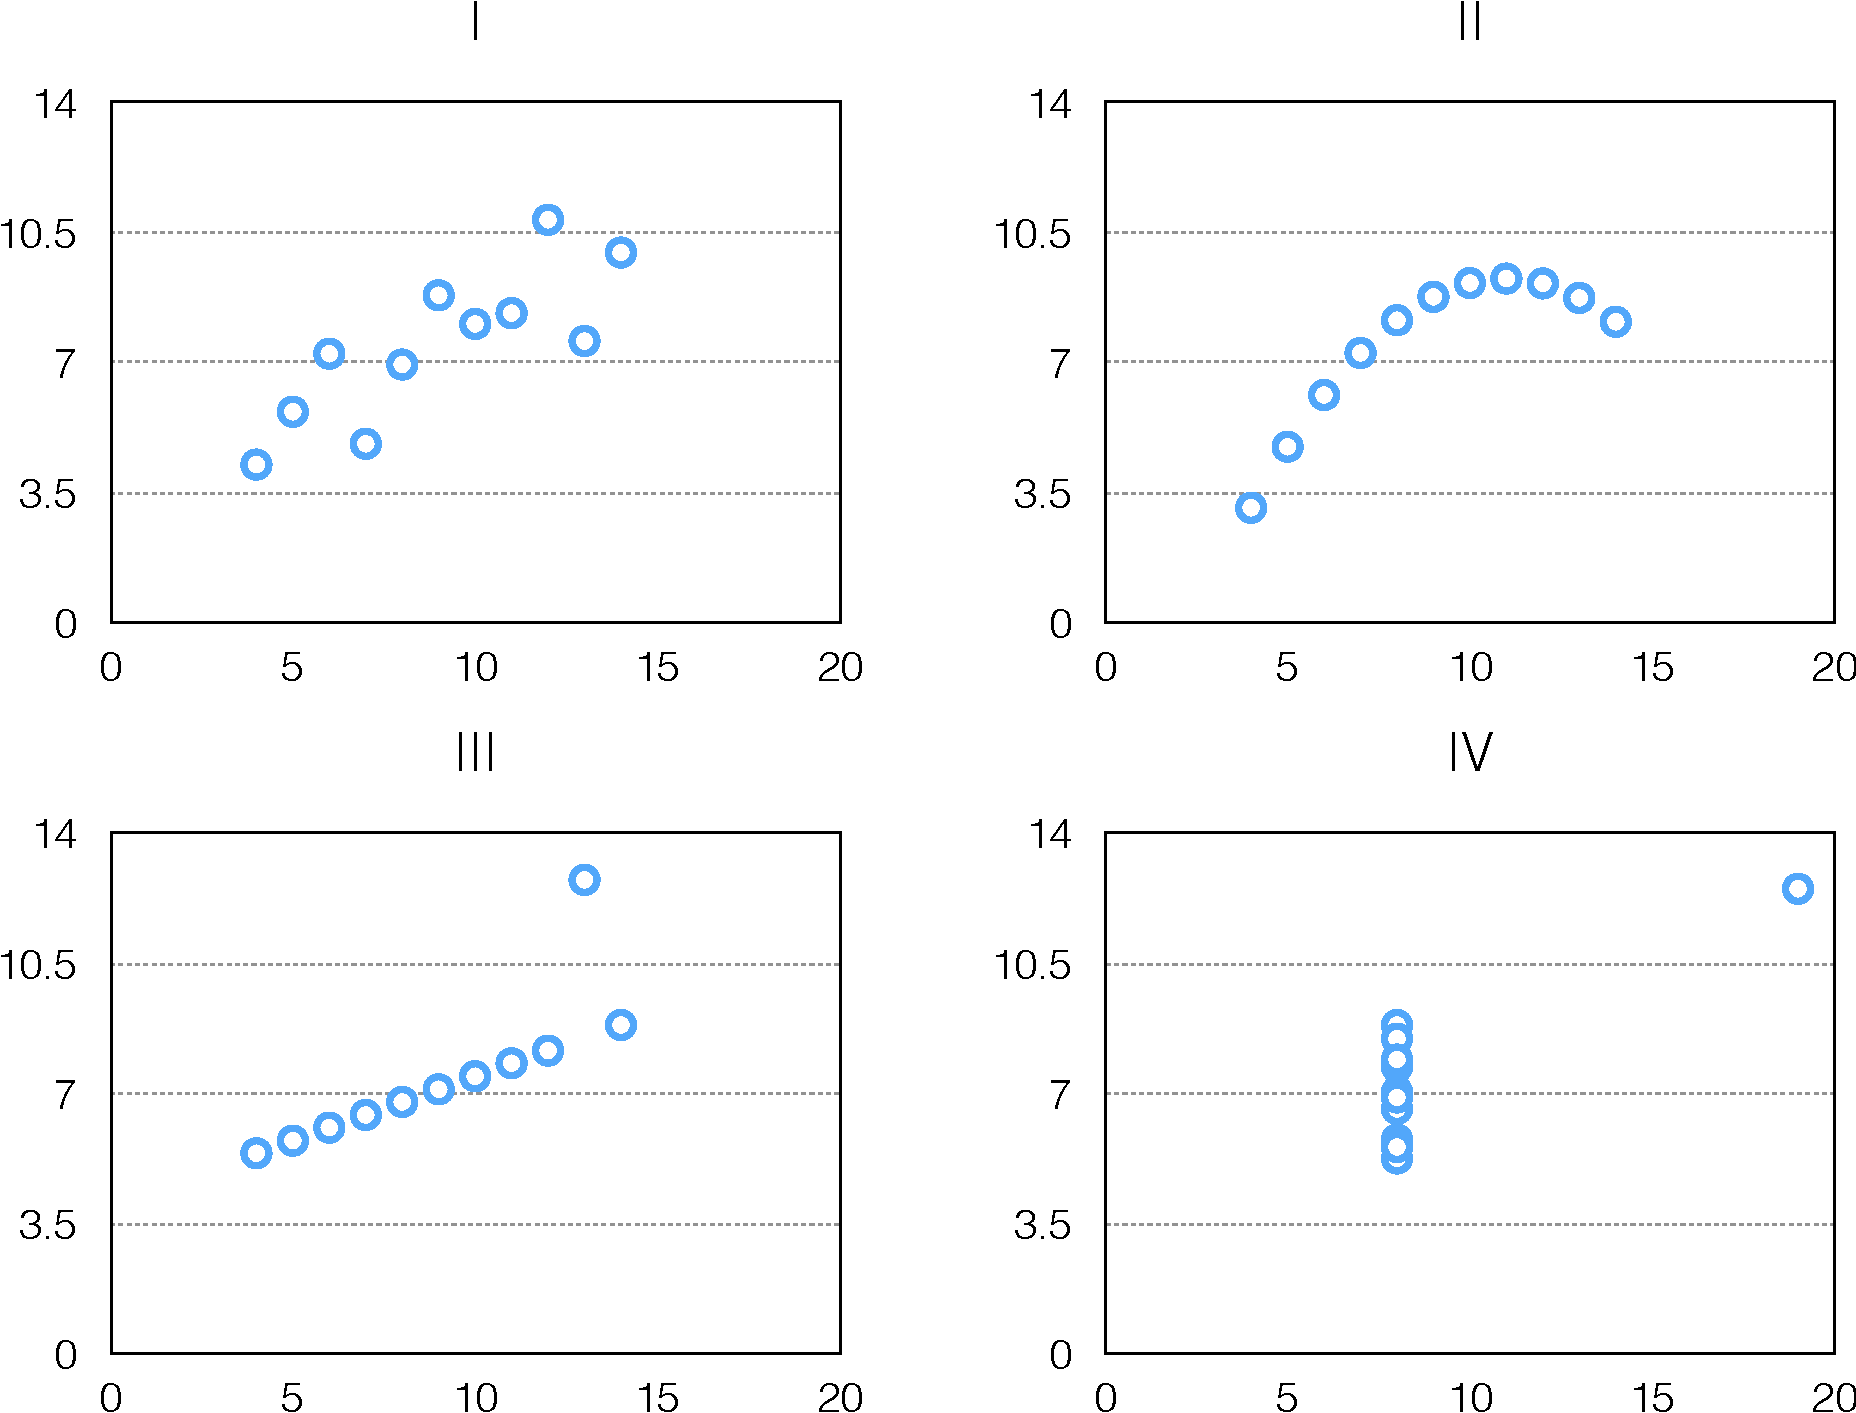
\includegraphics[width=0.8\linewidth]{figures/anscombes_quartet}
  \caption{\textbf{Anscombe's quartet.} Statistician F. Anscombe constructed these four data series to stress the importance of plotting the data before computing its summary statistics. These four sets of data points are indistinguishable when considering their $x$ and $y$ mean, variance, correlation, and linear regression, yet are strikingly different when visualized.}
  \label{fig:intro:anscombe}
\end{figure}


Visualization is an important first step when working with a new set of data as it provides the means to assess the overall shape of the data, its distribution, and to detect outliers. Anscombe's quartet~\cite{anscombe} succinctly demonstrates the importance of viewing the data before analyzing it: four datasets have the same $x$ and $y$ mean and variance, Pearson's correlation and fit the same regression line, yet are strikingly different (Figure~\ref{fig:intro:anscombe}). We see visualization as the means to generate new hypotheses that are then tested and validated through domain-specific algorithms and statistical models.


%%%%%%%%%%%%%%%%%%%%%%%%%%%%%%%%%%%%%%%%%%%%%%%%%%%%%%%%%%%%%%%%%%%%%%%%%%%%%%%
%%%%%%%%%%%%%%%%%%%%%%%%%%%%%%%%%%%%%%%%%%%%%%%%%%%%%%%%%%%%%%%%%%%%%%%%%%%%%%%
%%
%%
%%
%% Part 1 -- visualizaiton for biological data
%%
%%
%%
%%%%%%%%%%%%%%%%%%%%%%%%%%%%%%%%%%%%%%%%%%%%%%%%%%%%%%%%%%%%%%%%%%%%%%%%%%%%%%%
%%%%%%%%%%%%%%%%%%%%%%%%%%%%%%%%%%%%%%%%%%%%%%%%%%%%%%%%%%%%%%%%%%%%%%%%%%%%%%%
\part{Visualization approaches for biological data}
\label{part:vis}



%%%%%%%%%%%%%%%%%%%%%%%%%%%%%%%%%%%%%%%%%%%%%%%%%%%%%%%%%%%%%%%%%%%%%%%%%%%%%%%
%%
%% Coral --
%%
%%%%%%%%%%%%%%%%%%%%%%%%%%%%%%%%%%%%%%%%%%%%%%%%%%%%%%%%%%%%%%%%%%%%%%%%%%%%%%%
\chapter{Interfaces for evaluation and comparison of ensembles of classification results}
\label{chapter:coral}

  Clustering has become a standard analysis step for many types of biological data, \eg~interaction networks, gene expression, and metagenomic abundance. In practice, it is possible to obtain a large number of contradictory clusterings by varying which clustering algorithm is used, which data attributes are considered, how algorithmic parameters are set, and  which near-optimal clusterings are chosen. It is a difficult task to sift though such a large collection of varied clusterings to determine which clustering features are affected by parameter settings or are artifacts of particular algorithms and which represent meaningful patterns. Knowing which items are often clustered together helps to improve our understanding of the underlying data and to increase our confidence about generated modules.

  In this chapter, we discuss the design decisions and the implementation of \Coral, an application for interactive exploration of ensembles of classification results and clusterings. We discuss how each visual component in \Coral tackles a specific question related to clustering comparison and provide examples of their use. We also show how \Coral could be used to visually and quantitatively compare clusterings with a ground truth clustering. 

  We showcase how to use \Coral on a collection of clusterings for a protein interaction network of \textit{Arabidopsis thaliana}. We find that the clusterings vary significantly and that few proteins are consistently co-clustered in all clusterings, and use \Coral's core identification to identify these consistent protein subgroups. Our case study shows that several clusterings should typically be considered when evaluating clusters of genes, proteins, or sequences, and Coral can be used to perform a comprehensive analysis of these clustering ensembles.

  The work presented in this chapter has appeared as a publication in BMC Bioinformatics~\cite{Filippova2012} and was presented at ISMB 2012 as a poster. The software is available as a standalone Java application and can be downloaded from \url{https://github.com/lynxoid/coral}.

%%%%%%%%%%%%%%%%%%%%%%%%%%%%%%%%%%%%%%%%%%%%%%%%%%%%%%%%%%%%%%%%%%%%%%%%%%%%%%%
\section{Background and related work}



  Collections of protein interactions, gene expression vectors, metagenomic samples, and gene sequences containing thousands to hundreds-of-thousands of elements are now being analyzed routinely. 
% 
  % XXX more detail on the size of the problem. 
% 
  Clustering is often used to condense such large datasets into an understandable form: it has been successfully used on protein-protein interaction (PPI) networks to discover protein complexes and predict protein function, \eg~\cite{Sharan2007}; on gene expression data to find patterns in gene regulation and essential cell processes, \eg~\cite{Ulitsky2010}; and on metagenomic samples to identify new species, compare them to existing clades, evaluate the diversity of a population, and suggest interdependencies between them~\cite{Chatterji2007, White2010}. In other words, clustering has become a ubiquitous part of analysis for large biological datasets.

  % Introduce the problem.

  There are many clustering algorithms available for numerical and network data, \eg~\cite{VanDongen2000, Bader2003, Clauset2004, Adamcsek2006, Blondel2008, Ahn2010, Jiang2010, Rhrissorrakrai2011}. Each algorithm, and choice of its parameters, results in different clusterings. Sometimes, clustering algorithms must resolve ties when generating modules or may be randomized. Consequently, a single clustering algorithm may produce diverse partitions on the same data~\cite{Navlakha10}. Clusterings may also change when the underlying data becomes increasingly noisy or displays variation under different conditions (such as varying gene expression levels). In addition, considering many optimal and near-optimal partitions has been shown to improve the understanding of module dynamics and the strength of relationships between individual items~\cite{Duggal2010, Lewis2010, Langfelder2008, Hopcroft2004}. Such clusterings may offer drastically different perspectives on the data, where assessing the commonalities and differences is of great interest.

  % existing solutions

  There are several ways in which the problem of diverse clusterings has been addressed. Some tools rely on a single clustering only and focus on module quality assessment, \eg~\cite{Yu2007a, Hibbs2005}. Comparing two or more clusterings at a time is usually done by computing a single metric, such as the Jaccard or Rand index~\cite{Thalamuthu2006}, to compare clusterings side-by-side~\cite{Seo2007a} or in a dendrogram~\cite{Laderas2007}. These approaches can easily compare a pair of clusterings, but are not extendable to greater number of clusterings. Another approach is to aggregate multiple partitions into a consensus clustering~\cite{strehl02, Monti2003a} without delving into the differences between individual clusterings and, thus, disregarding possibly important information about the clusterings. Finally, some approaches have made steps towards visual examination of multiple clusterings: King and Grimmer~\cite{Grimmer2011} compare clusterings pairwise and project the space of clusterings onto a plane to visualize a clustering landscape, and Langfelder et al.~\cite{Langfelder2011} investigate ways to compare individual modules across multiple conditions. However, none of these approaches offer a platform for a multi-level analysis of ensembles of diverse clusterings.


%%%%%%%%%%%%%%%%%%%%%%%%%%%%%%%%%%%%%%%%%%%%%%%%%%%%%%%%%%%%%%%%%%%%%%%%%%%%%%%
\section{Interface design}

% overview -- shows Coral layout
  \begin{figure}[htb!]
    \centering
    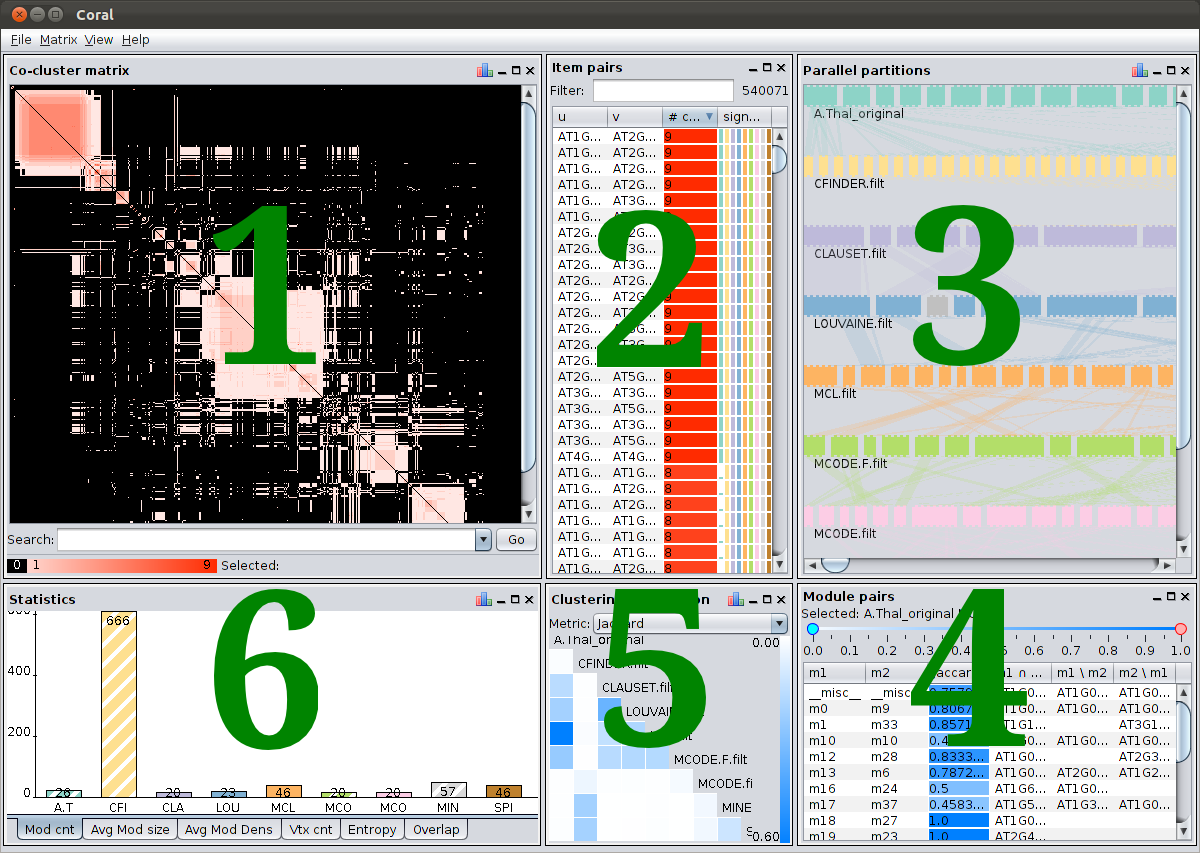
\includegraphics[width=\linewidth]{figures/coral_overview.png}
    \caption{\textbf{Coral overview.} Coral views in a clockwise direction: co-cluster matrix (1), pairs table (2), parallel partitions plot (3), module-to-module table (4), ladder (5), overview statistics (6). Users may rearrange the individual views or close them to focus on fewer visualizations at a time. Data: \Athal clusterings.}
    \label{fig:coral:overview}
  \end{figure}


  In \Coral's design, we followed the visualization mantra coined by Shneiderman~\cite{Shneiderman1996}: overview, zoom-and-filter, details-on-demand. At the overview level, \Coral displays dataset statistics and highlights the most similar and dissimilar clusterings; at the mid-level, ``zoomed-in,'' analysis explains similarities between clusterings through module comparison; the low-level analysis compares co-clustering patterns at the level of individual data items: the genes, proteins, or sequences. The displays are coordinated~\cite{North2000} so selecting data in one of the views highlights the corresponding items in the other views (see Figure~\ref{fig:coral:overview}).


  Coral works with modules --- groups of items closely related to one another according to some metric or property. For example, modules can constitute a collection of genes that get co-expressed together or proteins forming a complex. A clustering is a collection of modules and usually is an output of a clustering algorithm. Users may also choose to group data according to attributes that come with the data such as cellular component or molecular function GO terms and use that partition as a clustering. Users may combine data from different experiments and across species so long as the data items that the user treats as homologous have the same IDs across the dataset.



  \Coral takes as an input the module files where each file represents a single clustering, and each line in the file contains a list of data items (proteins, genes, or sequence ids) from a single module, \eg~as produced by MCL, the clustering algorithm by van Dongen~\cite{VanDongen2000}. \Coral aggregates and visualizes these data through several connected displays, each of which can be used to answer specific questions about the clusterings. Below, we examine a few such questions and describe how \Coral's visualizations help to answer them.

  %%%%%%%%%%%%%%%%%%%%%%%%%%%%%%%%%%%%%%%%%%%%
  %%
  %% Subsection
  %%
  %%%%%%%%%%%%%%%%%%%%%%%%%%%%%%%%%%%%%%%%%%%%

  \subsection{Summary statistics}



\begin{figure}[h]
    \centering
    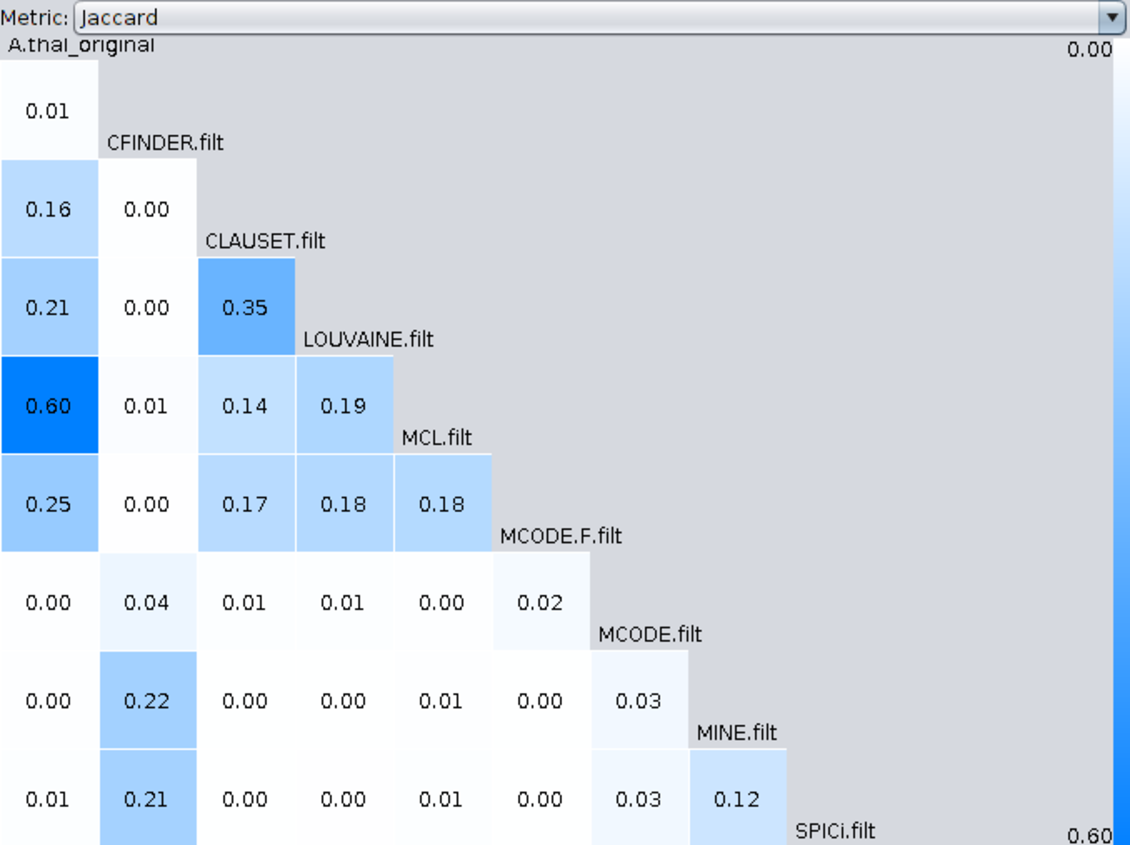
\includegraphics[width=0.60\linewidth]{figures/coral_ladder}
    \caption{\textbf{All-to-all clustering comparison in a ladder widget.} The ladder represents  a lower triangle of an all-to-all matrix where each cell $(i, j)$ holds a score for similarity between clusterings $K_{i}$ and $K_{j}$. Users can choose between several comparison metrics by toggling a dropdown above the ladder. Every cell is color-coded, with darker colors indicating more similarity between the pair} 
    \label{fig:coral:ladder}
  \end{figure}


  %
  To gain a quick overview of their collection of clusterings, \Coral users may start the analysis by reviewing basic statistics about their data (Figure~\ref{fig:coral:overview}, area 6): number of modules per clustering, average module size, module coverage, clustering entropy~\cite{Meila2003}:
  %
  \[
  H(K) = - \sum_{m_i \in K} p_i \log_2 p_i,
  \]
  %
  where $K$ is a clustering and $m_i$ is a module in $K$, $p_i = |m_i| / |K|$, and percentage of data items that ended up in the overlapping modules. Questions such as ``Do clusterings have the same number of modules?''\@ and ``Are module sizes evenly distributed?''\@ can be easily answered through these statistics. Each statistic is shown as a bar chart, and every clustering is associated with a unique color that is used consistently throughout \Coral to identify the clustering anywhere in the system. If a clustering contains overlapping modules, the corresponding bar in the chart is striped as opposed to a solid bar for the clusterings containing no overlapping modules (see Figure~\ref{fig:coral:overview}).

  %%%%%%%%%%%%%%%%%%%%%%%%%%%%%%%%%%%%%%%%%%%%
  %%
  %% Subsection
  %%
  %%%%%%%%%%%%%%%%%%%%%%%%%%%%%%%%%%%%%%%%%%%%
  \subsection{Assessing similarity of clusterings}
  %
  % introduce ladder 
  \Coral computes similarity scores between all clusterings and visualizes the lower triangle of the similarity matrix in a ladder widget (Figure~\ref{fig:coral:ladder}). The ladder compactly displays similarity scores for every pair of clusterings in the ensemble allowing for precise comparisons. The ladder is color-coded as a heatmap with more intense blue cells corresponding to higher similarity scores and paler cells corresponding to low scores. Clicking a cell updates the contents of a module-to-module comparison widget (see next subsection).


  \Coral offers several choices of similarity measures to compare partitions. Four of the measures are based on pair counting, two measures use information theory to quantify diversity of the clusterings, and the remaining measures rely on set matching to produce a score. Pair counting measures use the following four quantities to compute a score:

  % pair counting quantities
  \begin{itemize}
  \item $a$ --- pairs of items placed in a module together in clustering $K_{i}$ and $K_{j}$,
  \item  $b$ --- pairs of items placed in a module together in $K_{i}$, but not in $K_{j}$,
  \item $c$ --- pairs of items placed in separate modules in $K_{i}$, but in the same module in $K_{j}$,
  \item $d$ --- pairs of items placed in separate modules in both $K_{i}$ and $K_{j}$.
  \end{itemize}

  $K_i$ and $K_j$ are two clusterings, the measures of similarity between them are as follows:
  %
  \begin{enumerate}
    \item Jaccard coefficient for sets of sets:
    %
    \[
    J(K_i, K_j) = a / (a + b + c);
    \]
    %
    Jaccard coefficient is symmetric and ignores quantity $d$ instead focusing on the pairs of items that were in the same module in either $K_i$ or $K_j$.

    \item Mirkin coefficient:
    %
    \[
    M(K_i, K_j) = 2(b + c),
    \]
    %
    a symmetric, yet unbounded metric.
    % Mirkin coefficient is symmetric, but is not a metric.

    \item Rand index:
    \[
    R(K_i, K_j) = (a + d) / (a + b + c + d)
    \]
    is not symmetric.

    \item Fowlkes-Mallows index:
    %
    \[
    FM(K_i, K_j) = \sqrt{a / (a + b) a / (a + c) },
    \]
    %
    where higher values correspond to greater similarity between the clusterings.

    \item Mutual information (MI):
    %
    \[
    I(K_i,K_j) = \sum_{m_k \in K_i} \sum_{m_l \in K_j} p_{kl} 
        \log \frac{ p_{kl} }{ p_k p_l }
    \]
    %
    where $m_k$ and $m_l$ are modules in their corresponding clusterings and probabilities are calculated as follows: $p_k = |m_k| / |K_i|$, $p_l = |m_l| / |K_j|$, $p_{kl} = |m_k \cup m_l| / (|K_i| + |K_j|)$. Mutual information is symmetric, but is not a metric, although its version, variation of information, can be combined with joint entropy $H(K_i, K_j)$ to become one.

    \item Variation of information (VI):
    %
    \[
    VI(K_i,K_j) = H(K_i, K_j) - I(K_i, K_j)
    \]
    %
    where $H(K_i, K_j)$ is a joint entropy. VI is a metric.

    \item Purity index:
    %
    \[
    P(K_i,K_j) = \frac{ \sum_{m_k \in K_i} \argmax_{m_l \in K_j} |m_k \cap m_l| }{N},
    \]
    %
    where $N$ is the number of clustered data items in $K_i$. For every module in $K_i$, purity index finds the module in $K_j$ that overlaps with $m_k$ the most therefore capturing the maximum amount of overlap between modules in $K_i$ and $K_j$. The index is not symmetric.

    \item Inverse purity index:
    %
    \[
    IP(K_i,K_j) = \frac{ \sum_{m_l \in K_j} \argmax_{m_k \in K_i} |m_k \cap m_l| }{N},
    \]
    %
    is similar to purity, but captures the maximum amount of overlap as viewed from $K_j$'s perspective. The index is not symmetric.

    \item F-measure~\cite{Meila2003}:
    %
    \[
    F(K_i,K_j) = \frac{ \sum_{m_k \in K_i} |m_k| \argmax_{m_l \in K_j} f(m_k, m_l) }{N/2},
    \]
    %
    where $N$ is the number of data items in $K_i$. Precision between two modules $m_k$ and $m_l$ is defined as $p(m_k, m_l) = |m_k \cap m_l| / |m_k|$ and is an asymmetric measure with recall define as its opposite: $r(m_k, m_l) = p(m_l, m_k)$. The f-score between two modules is $f(m_k,m_l) = r(m_k, m_l) p(m_k, m_l) / ( r(m_k, m_l) + p(m_k, m_l) )$.

  \end{enumerate}

  In \Coral, certain metrics are faster to compute than others: for example, counting metrics (1-4) take on the order of $O(1)$ for a single clustering pair rather than $O(modules^2)$ $O(n^2)$ since they are implemented using low-level bit operations on the bit-wise representation of a clustering. Low computational cost for computing these metrics allows Coral to scale to hundreds of moderately-sized clusterings where all-to-all comparison would require computation of $O(k^2)$ individual similarity values.

  %%%%%%%%%%%%%%%%%%%%%%%%%%%%%%%%%%%%%%%%%%%%
  %%
  %% Subsection
  %%
  %%%%%%%%%%%%%%%%%%%%%%%%%%%%%%%%%%%%%%%%%%%%
  \subsection{Module similarity across clusterings}
  \label{sec:modules}

  As a follow-up to finding a highly similar pair of clusterings, users can review the similarities between their individual modules. Is a group of interacting genes preserved between the two stages in the cell life cycle? Is there a match for a given protein complex in the PPI network of another species? Module-to-module comparison table helps to answer these questions to explains in detail what contributed to the clustering similarity at a  module level.

  For a given pair $K_1, K_2$ of clusterings, \Coral calculates the Jaccard similarity $J = |m^{1}_{i} \bigcap m^{2}_{j}| / |m^{1}_{i} \bigcup m^{2}_{j} |$ between every module $m^{1}_{i} \in K_1$ and $m^{2}_{j} \in K_2$ thus capturing the amount of overlap between the two modules. For every such module pair, \Coral displays the pair's Jaccard score and items in the union, intersection, left and right set differences. All module pairs are organized in a sortable table (see Figure~\ref{fig:coral:modules}). The slider above the table allows the user to filter out module pairs for which the Jaccard score is outside the slider's range allowing users to focus on highly similar (or dissimilar) modules. Although module-to-module analysis is possible with the parallel partitions plot (discussed below), the table offers a sortable and filterable view of the same data while supplying additional information (\eg~Jaccard index). The module-to-module table shows only the module pairs with some overlap and easily scales to hundreds of modules, thereby offering a more compact and easily navigable alternative to a confusion matrix (\eg\@ as used in~\cite{Langfelder2011}).

  % module to module comparison table
  \begin{figure}[ht]
    \centering
    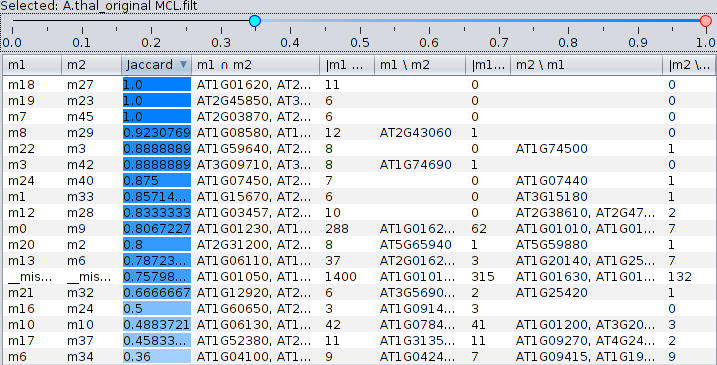
\includegraphics[width=0.8\linewidth]{figures/coral_modules}
    \caption{\textbf{Module-to-module comparison for two clusterings.} When users decide to focus on a pair of clusterings, they may explore all pairs
    of modules in a sortable table. Each module pair is shown against its Jaccard
    score, and lists of items in the module intersection, left and right
    differences. Users can filter the table rows by Jaccard score to only show rows
    within a given similarity range by adjusting the slider above the table. Cells
    holding the Jaccard scores are color-coded to indicate similarity.}
    \label{fig:coral:modules}
  \end{figure}

  %%%%%%%%%%%%%%%%%%%%%%%%%%%%%%%%%%%%%%%%%%%%
  %%
  %% Subsection
  %%
  %%%%%%%%%%%%%%%%%%%%%%%%%%%%%%%%%%%%%%%%%%%%

  \subsection{Module persistence across clusterings}

  The ability to track individual items and whole modules across multiple clusterings provides a high level of abstraction in clustering analysis: modules may split and merge as users switch from clustering to clustering. To afford an exploration at the module level, we have developed a parallel partitions plot --- an extension of a parallel sets plot used in the analysis of categorical multivariate data~\cite{Kosara2006}. The parallel partitions plot represents each clustering as a horizontal band. The blocks comprising each bands represent modules, with the width of a block proportional to the number of items in that module. Semi-transparent parallelograms between clusterings connect data items with the same name. That is, each item in a clustering will be connected to its copy in the band immediately below it (see Figure~\ref{fig:coral:parsets}).

  % parallel partitions figure
  \begin{figure}[htb!]
    \centering
    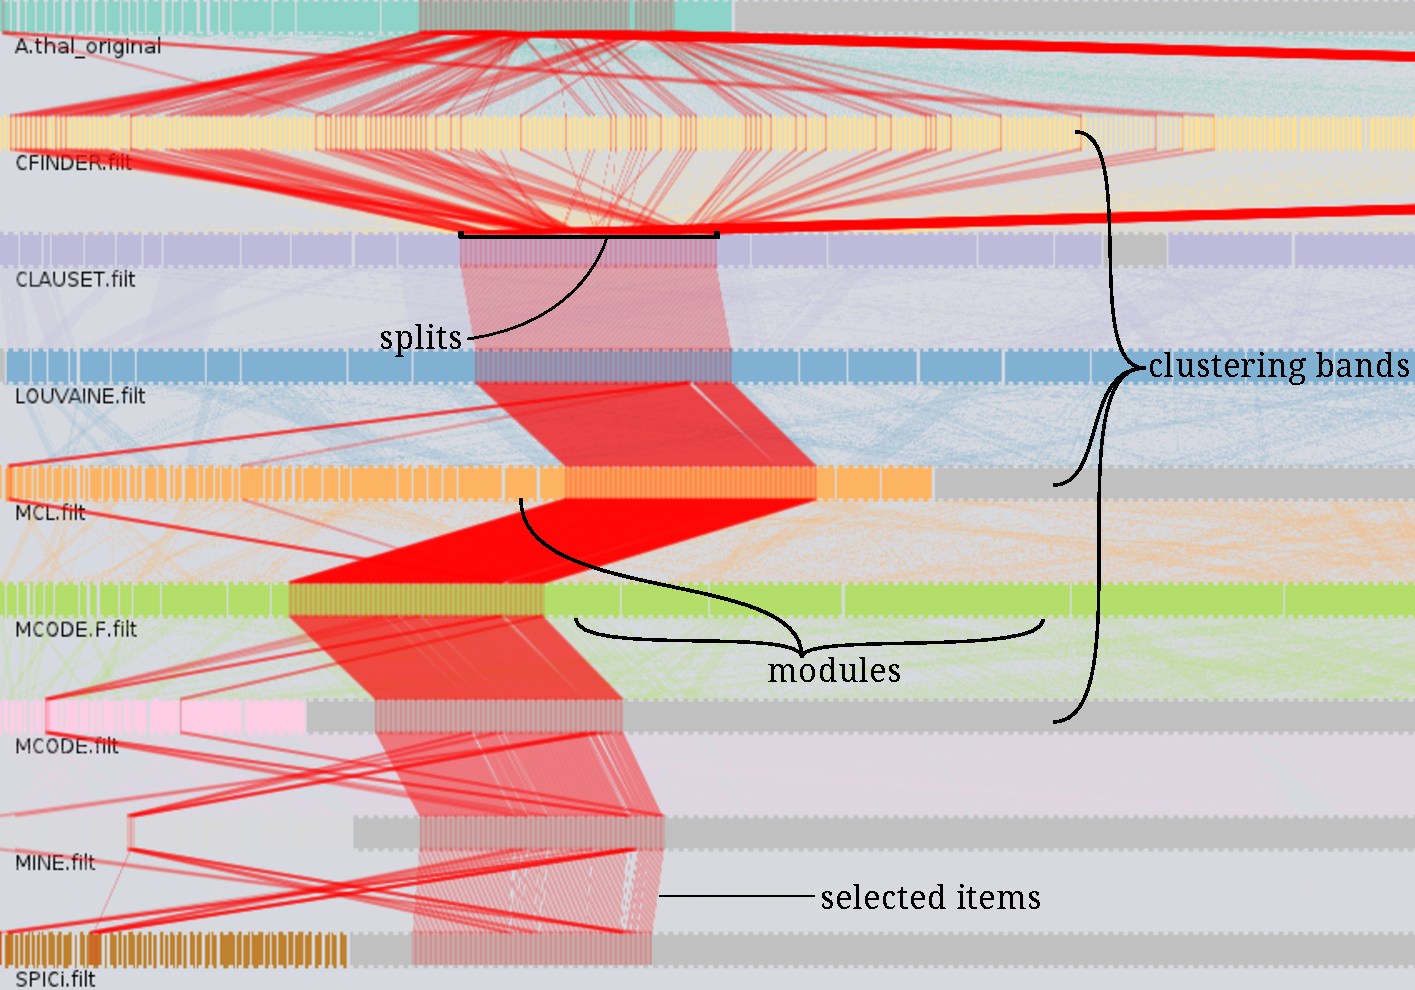
\includegraphics[width=\linewidth]{figures/coral_parsets}
    \caption{\textbf{Parallel partitions maps modules between clusterings.} Horizontal bands represent partitions, and modules are separated by blank spaces. Semi-transparent bands connect the same items from different
   clusterings. Red traces highlight selected items across all partitions and show how modules split and merge. Here, the user has selected a group of 215 proteins that belong to the largest core in the ensemble of clusterings for \Athal PPI network. The \texttt{Louvaine}, \texttt{Clauset}, \texttt{MCL}, and \texttt{MCODE.F} clusterings assign all of the selected proteins to a single
   module. For other clusterings, most of the selected proteins are placed in a
   grab bag region of items that were not contained in any module (shown in gray).}
    \label{fig:coral:parsets}
  \end{figure}

  The parallel partitions plot allows users to track individual items and whole modules across all partitions. To see whether a module splits or merges in other clusterings, users can select a module with a mouse while holding a shift key to highlight its members in every clustering in the plot (see red traces in Figure~\ref{fig:coral:parsets}). Similarly, users may select individual items and trace them through every clustering band. The selections made in the parallel partitions plot propagate to other views making it easy to track the same group of items throughout the application. The plot is zoomable --- users may zoom in to focus on a few items at a time or zoom out to see global trends across the ensemble. When the zoom level permits it, the plot displays the item labels.

  % co-occurrence matrixes
  \begin{figure}[ht]
    \centering
    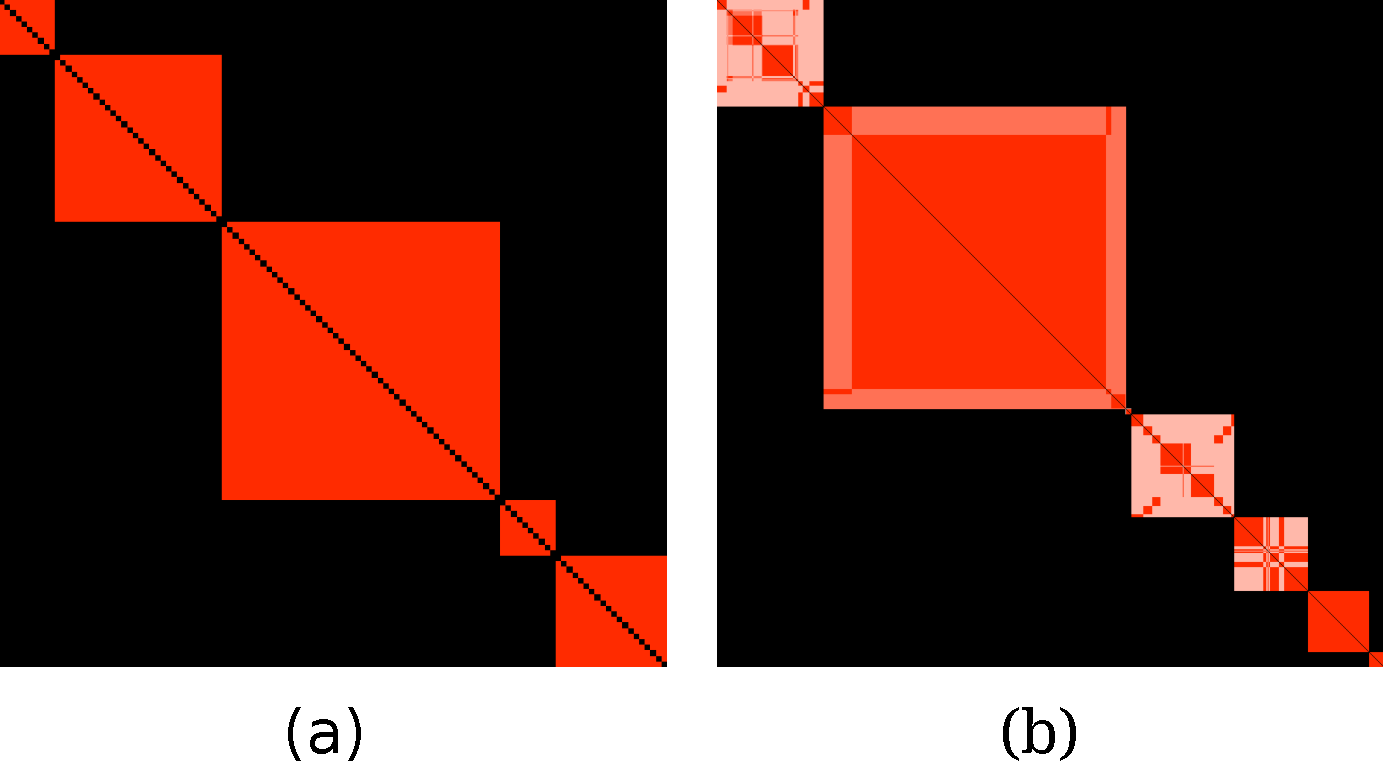
\includegraphics[width=0.7\linewidth]{figures/coral_matrices}
    \caption{\textbf{Co-cluster matrices.} (a) A co-cluster matrix of three identical decompositions forms blocks on
    the diagonal with only red cells indicating that all three clusterings agreed
    (synthetic data). (b) Big modules were broken up into smaller modules to form
    new clusterings (four \texttt{Hybrid} decompositions from the Langfelder
    study~\cite{Langfelder2008}).}
    \label{fig:coral:matrices}
  \end{figure}

  The order of items in the clustering bands matches the order of items in the
  co-cluster matrix (discussed below) as closely as possible, while at the same
  time attempting to minimize the amount of crossover between the parallelograms
  connecting items in the consecutive clusterings. However, the items in the bands
  must be placed inside their respective modules. We
  discuss an algorithm that finds a good ordering of items in the
  clustering bands in the Methods section.

  %%%%%%%%%%%%%%%%%%%%%%%%%%%%%%%%%%%%%%%%%%%%
  %%
  %% Subsection
  %%
  %%%%%%%%%%%%%%%%%%%%%%%%%%%%%%%%%%%%%%%%%%%%

  % section's math
  \newcommand{\Mplus}{$A^{+}$~}

  %\subsection*{co-cluster matrix}
  \subsection{Co-clustering patterns over all items}

  A single clustering assigns a data item $v$ to a module defining its \textit{cohort} --- a set of items in the same module as $v$. Knowing the item's module helps in assigning function to unknown proteins~\cite{Bader2003} and novel genes~\cite{Ulitsky2010}; knowing that the item's cohort is consistent across many clusterings increases the confidence of such predictions.

  % introduce co-cluster matrix

  In \Coral, pairwise co-cluster memberships are aggregated in a \textit{co-cluster matrix}
  ~\cite{Monti2003a}. Given a single clustering $K$, $n = |K|$, we define an
  $n \times n$ matrix $A^{K}$ to be $K$'s co-cluster matrix where its entries
  $a_{ij}^{K}$ are:
  %
  \[
   a_{ij}^{K} =
    \begin{cases}
  0 & \text{$v_{i}$ and $v_{j}$ are in different modules in $K$}\\
  1 & \text{$v_{i}$ and $v_{j}$ are in the same module in $K$}.\\
    \end{cases}
  \]

  For some item pairs, co-clustering may be an artifact of a tie-breaking policy or a choice of an algorithm parameter: such item pairs may only co-cluster in few clusterings. On the other hand, we would like to know whether there were item pairs that co-clustered across most partitions in the ensemble. These cohort dynamics stand out if we sum up the co-cluster matrices to form a single matrix:
  %
  \[
   A^{+} = \sum_{t=1}^{k} A^{K_{t}},
  \]
  %
  where $A^{K_{t}}$ is a co-cluster matrix for a clustering $K_{t}$ and $k$ is the
  number of clusterings. Here, the $a_{ij}^{+}$ entries equal $k$ (the number of
  clusterings) for item pairs $(v_{i}, v_{j})$ that have co-clustered in all
  partitions suggesting a strong relationship between the items, and the low
  $a_{ij}^{+}$ values correspond to pairs that co-clustered in only a few
  clusterings and are more likely to have been assigned to the same module by
  chance. The cells are colored according to their values and vary from white
  (low values) to red (high values). Users may zoom in and out on the matrix to
  focus on areas of interest.

  % reordering, core extraction

  The co-cluster matrix is hard to read unless similar rows and columns are placed near each other. Reordering the rows and columns of \Mplus brings non-zero entries closer to the diagonal and exposes any modular structure (see Section~\ref{sec:coral:reordering}). When clusterings are highly similar, the reordered matrix will consist of blocks along the diagonal with high $a_{ij}^{+}$ values (Figure~\ref{fig:coral:matrices}). Clusterings that are very dissimilar produce reorderings similar to Figure~\ref{fig:coral:big_matrix} --- the diagonal blocks mostly contain low $a_{ij}^{+}$ values (colored white or light pink) with many entries away from the diagonal.

  % big reordered matrix w/ corresponding network vis
  \begin{figure}[htb!]
    \centering
    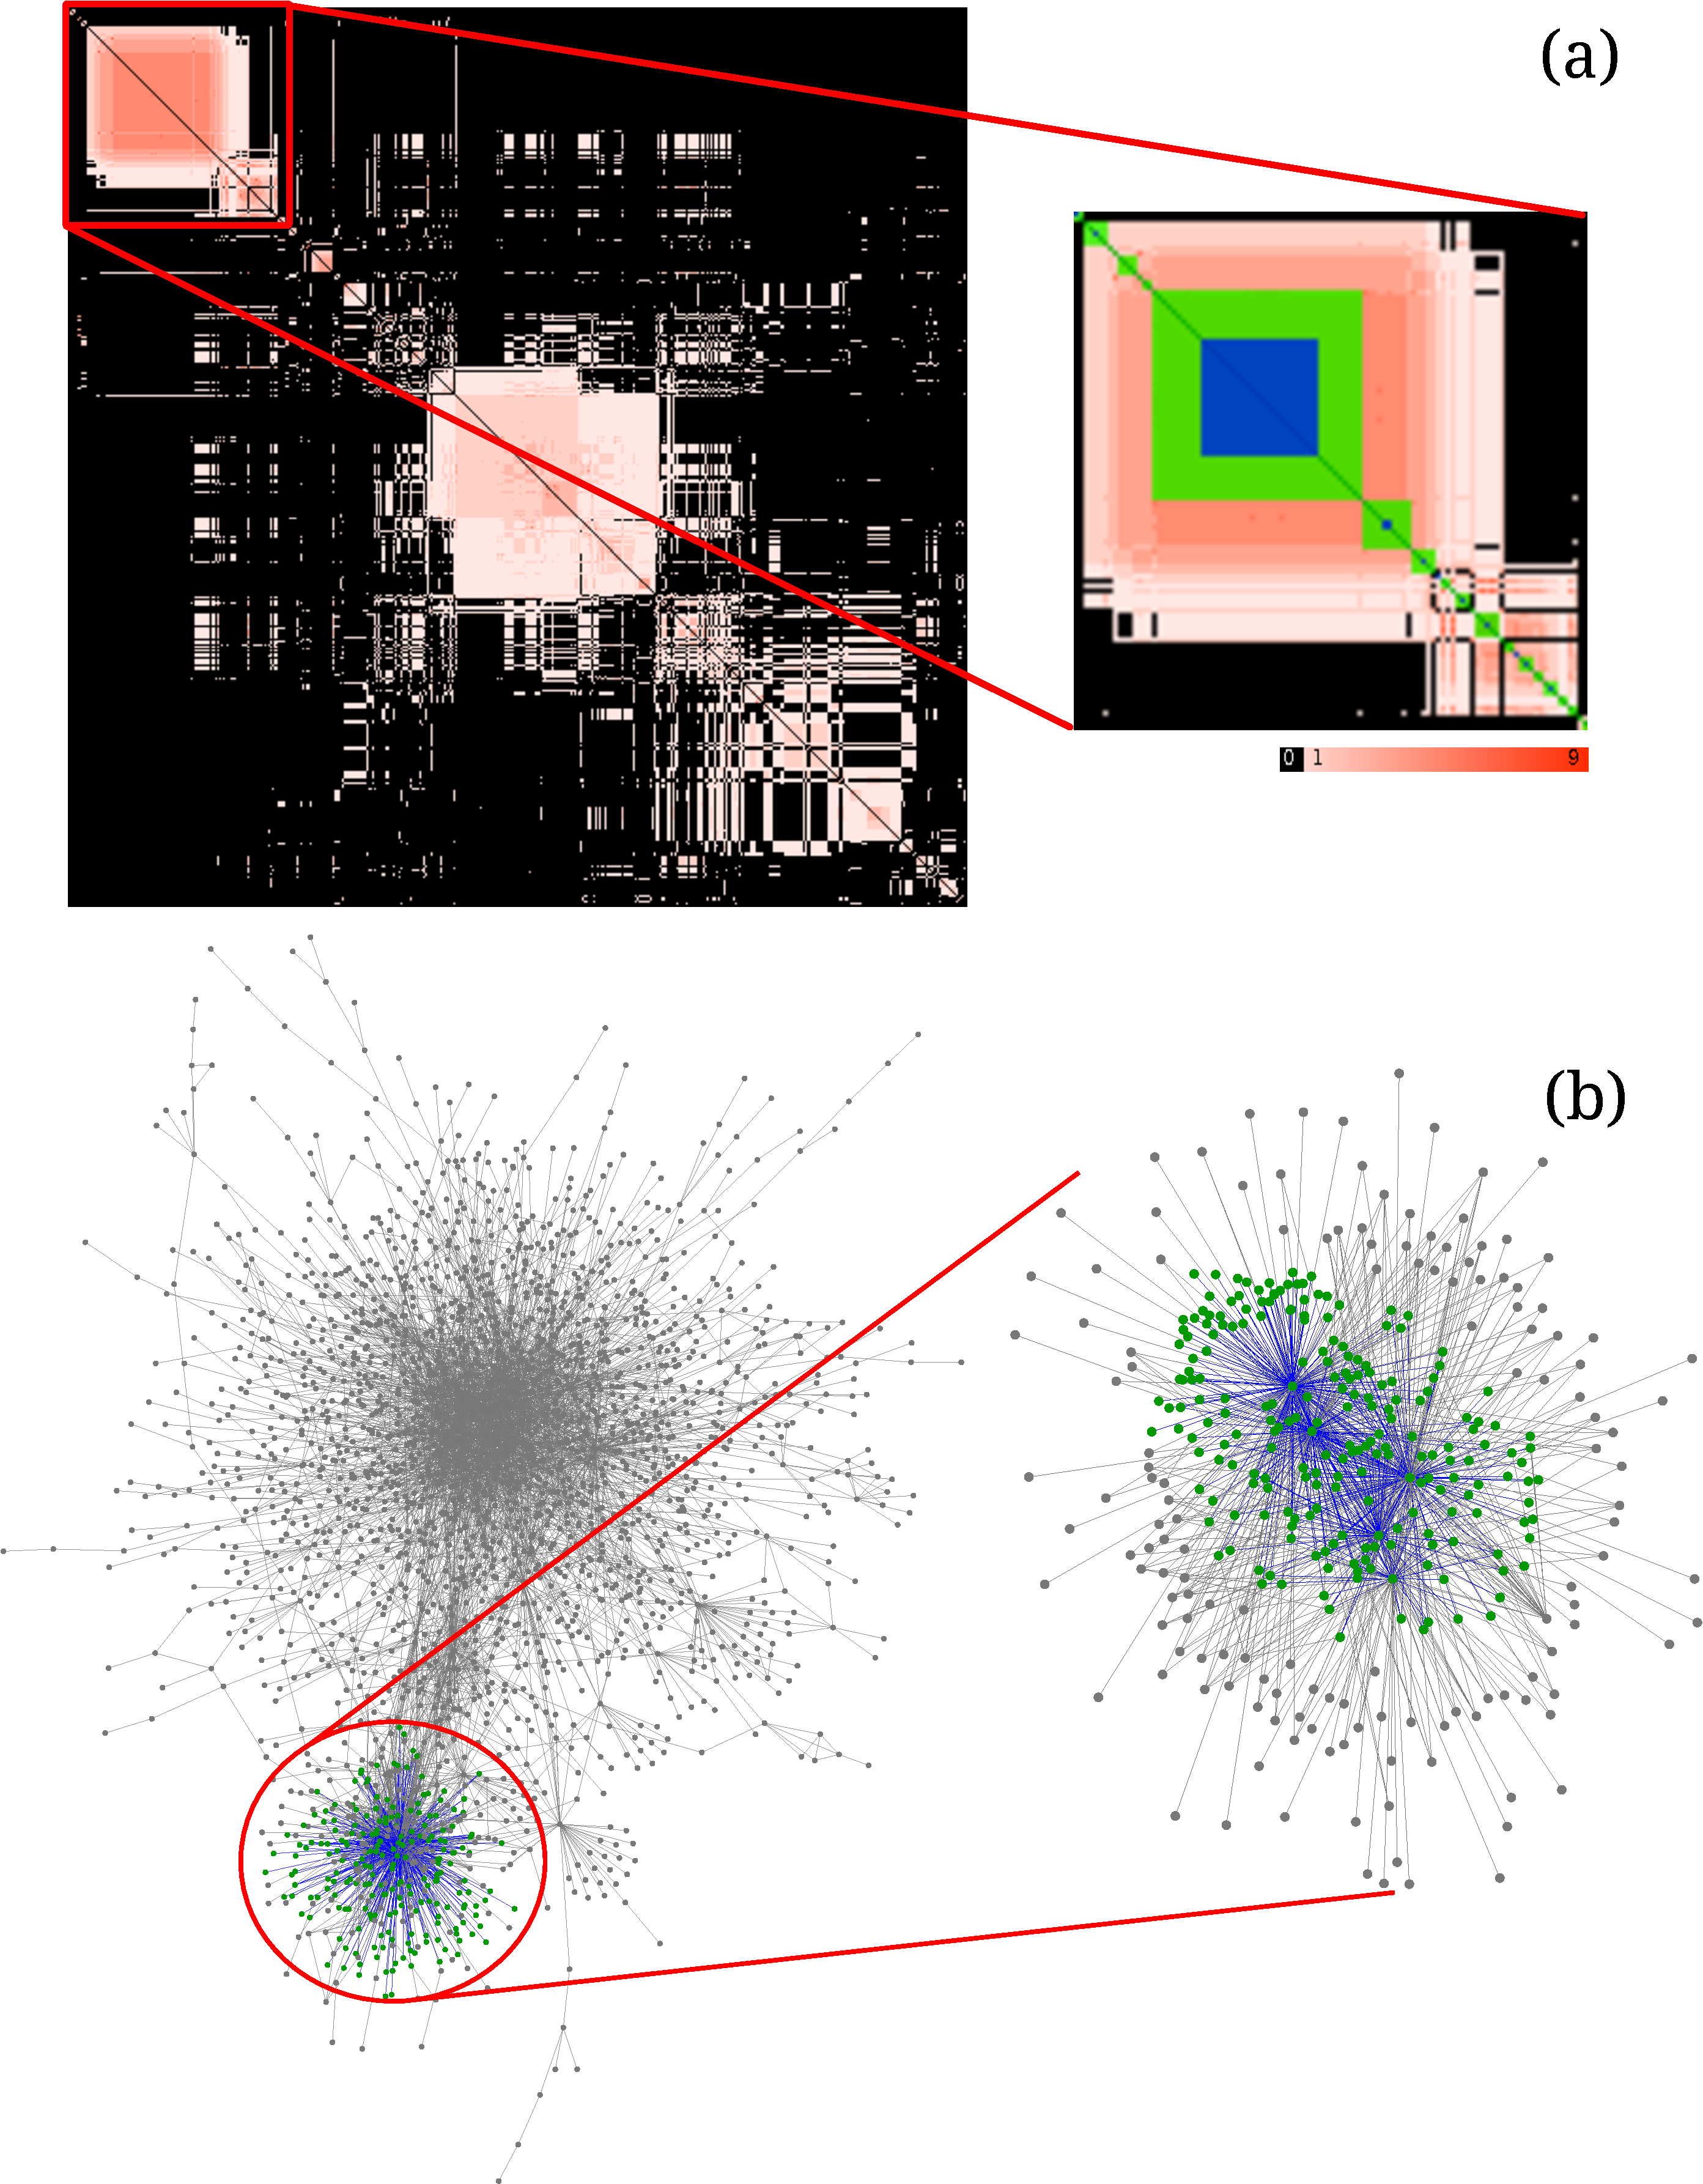
\includegraphics[width=0.6\linewidth]{figures/coral_vidal_matrix}
    \caption{\textbf{Reordered co-cluster matrix reveals co-clustering patterns.} (a) Values in the co-cluster matrix range from 1 (light pink) to 9 (red) for nine clusterings of the \Athal PPI network with 2402 proteins from~\cite{Vidal2011}. Pink regions represent item pairs that were placed in the same module by very few clusterings while regions of more saturated red represent proteins that co-clustered in most clusterings. Black indicates that the items never co-clustered. On the inset matrix, the matrix items under the green square formed a core. A large blue square overlay suggests that the core was tightly integrated into the rest of the network. (b) Left: nodes that formed a core in (a) are colored green, the edges between the nodes within the core are colored blue. The inset to the right shows an isolated view of the core nodes (green), edges between core nodes (blue), and nodes one hop away from the core nodes (gray). Green nodes share many edges with nodes outside of the core which resulted in the core's low cohesion.}
    \label{fig:coral:big_matrix}
  \end{figure}

  %%%%%%%%%%%%%%%%%%%%%%%%%%%%%%%%%%%%%%%%%%%%
  %%
  %% Subsection
  %%
  %%%%%%%%%%%%%%%%%%%%%%%%%%%%%%%%%%%%%%%%%%%%
  %\subsection*{Cores and periphery}
  \subsection{Subsets of items with the most persistent annotations across clusterings}
  \label{sec:cores}

  Groups of items that end up in the same module across many clusterings are of a particular interest because they represent the robust subclusters in the data. We call these commonly co-clustered sets \textit{cores}. Items in cores form the most trustworthy modules and indicate particularly strong ties between data items, increasing, for example, the confidence in protein complex identification~\cite{Luo2009} and gene annotation~\cite{Saha}.

  In a co-cluster matrix, most cores appear as contiguous blocks of high-value entries, although cores could ``wrap around'' being a two-dimensional projection of an $n$-dimensional data. \Coral finds the cores using a fast dynamic programming algorithm and highlights them within the co-cluster matrix (inset, Figure~\ref{fig:coral:big_matrix}a). When users provide clusterings derived from a network, \Coral can augment cores with an overlay showing each core's cohesion --- the ratio $E_\textrm{in} / E_\textrm{out}$ where $E_\textrm{in}$ is the number of edges within the core and $E_\textrm{out}$ is the number of edges that have one endpoint inside the core and another endpoint outside of it~\cite{Bailey1982}. When a core's cohesion is low, the blue overlay is smaller indicating that the core shares many connections with the rest of the network (Figure~\ref{fig:coral:big_matrix}b). Cores for which cohesion is high are more isolated from the rest of the network --- these cores are distinguishable by the blue overlays that almost cover the core.

  %%%%%%%%%%%%%%%%%%%%%%%%%%%%%%%%%%%%%%%%%%%%
  %%
  %% Subsection: Base clustering
  %%
  %%%%%%%%%%%%%%%%%%%%%%%%%%%%%%%%%%%%%%%%%%%%

  \subsection{Persistence of ground truth modules across clusterings}

  When validating new protein complexes or co-expressed gene modules, users may want to see how well their results match ground-truth clusterings such as protein complexes from MIPS~\cite{Mewes2011}, or sets of co-regulated genes from RegulonDB~\cite{Gama-Castro2011}. In \Coral, users may designate a single clustering as a \textit{base} --- a set of trusted modules with which other clusterings are expected to agree. When in this mode, \Coral will only highlight those cells in the co-cluster matrix that are within the modules of the base and gray out all other non-zero matrix cells to bring users' attention to the clustering in question. Figure~\ref{fig:coral:base_clust} shows an example of a co-cluster matrix with the base set to be the \Athal modules reported in~\cite{Vidal2011}.

  % showcasing base clustering feature
  \begin{figure}[!htb]
    \centering
    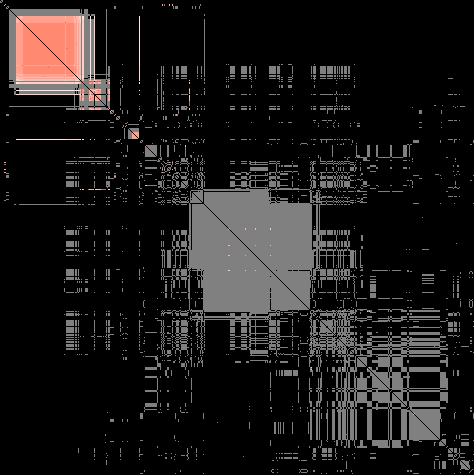
\includegraphics[width=0.7\linewidth]{figures/coral_base_matrix}
    \caption{\textbf{Base clustering mode for the co-cluster matrix.} The base clustering highlights only the item pairs that co-clustered within the selected clustering graying out the rest of the matrix. Base clustering helps users focus on comparisons with the selected clustering. In this figure, the colored areas represent the original 26 \Athal modules; their mostly pink hue indicates that their item pairs co-clustered in few clusterings. Large areas of gray indicate that many novel modules found by other clusterings were not found by the link clustering algorithm~\cite{Ahn2010}.}
    \label{fig:coral:base_clust}
  \end{figure}

  %%%%%%%%%%%%%%%%%%%%%%%%%%%%%%%%%%%%%%%%%%%%
  %%
  %% Subsection
  %%
  %%%%%%%%%%%%%%%%%%%%%%%%%%%%%%%%%%%%%%%%%%%%
  %\subsection*{Pairs table}
  \subsection{Co-clustering patterns of individual items}
  \label{sec:pairs_table}

  The co-cluster matrix displays the total number of times any two items were co-clustered, and the tooltips that appear after hovering over a matrix cell show a list of clusterings in which a given pair has been co-clustered. To facilitate sorting and search for particular item pairs, \Coral provides a companion table where each row represents a pair of data items and displays the number of times the items co-clustered along with the pair's \textit{signature}. The signature is a $k$-long vector where the $t^{th}$ element is 1 when both data items, say, proteins, have been placed in the same module in clustering $K_{t}$. If the pair's items were not in the same module in $K_{t}$, the $t^{th}$ element is set to 0.

  Visually, the signature's elements that are 1 are drawn as tall solid columns and zeros are represented by the short stumps using the same color for each clustering as used in the overview statistics and in the parallel partitions plot. Figure~\ref{fig:coral:signature} shows an example of two such pairs that have different co-cluster signatures suggesting that the relationship between the last two \Athal proteins is stronger than that of the first pair. Users can sort the rows by either the item name, the number of shared clusterings, or by the co-clustering signature. Users can also filter by the signatures to display only the rows matching a user's pattern.

  %co-clustering signatures
  \begin{figure}[!htb]
    \centering
    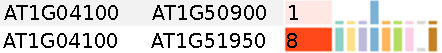
\includegraphics[width=0.4\linewidth]{figures/coral_item_pair}
    \caption{\textbf{Co-cluster signatures help track where two items have co-clustered.} Two rows from the pairs table for the \Athal dataset: each row starts with the two item IDs (here: \Athal proteins), followed by the number of times these two proteins were co-clustered, followed by a co-cluster signature that tells in which clusterings the two proteins were co-clustered. Clusterings order for this example: \Athal, \texttt{Clauset}, \texttt{CFinder}, \texttt{Louvain}, \texttt{MCL}, \texttt{MCODE.F}, \texttt{MCODE}, \texttt{MINE}, \texttt{SPICi}. Proteins AT1G04100 and AT1G51950 co-clustered in 8 clusterings. The two share many specific GO annotations: both are involved in auxin stimulus, localize to the nucleus, and participate in protein binding and sequence-specific DNA binding transcription factor activity. AT1G04100 and AT1G50900 were in the same module just once and shared no GO annotations suggesting that the relationship between these two proteins was of a more tenuous nature.}
    \label{fig:coral:signature}
  \end{figure}

\section{Algorithmic challenges}

  %%%%%%%%%%%%%%%%%%%%%%%%%%%%%%%%%%%%%%%%%%%%
  %%
  %% Subsection
  %%
  %%%%%%%%%%%%%%%%%%%%%%%%%%%%%%%%%%%%%%%%%%%%
  \subsection{Reordering the co-cluster matrix}
  \label{sec:coral:reordering}

  The order of rows and columns in the co-cluster matrix is critical to extracting meaningful information from it. Finding an optimal matrix reordering is NP-complete for almost any interesting objective. Algorithms for the optimal linear arrangement~\cite{Mueller} and bandwidth minimization~\cite{Lai1982} problems have been used to reorder matrices with considerable success; however, both approaches perform poorly for matrices that have many off-diagonal elements. After comparing several reordering algorithms using the bandwidth and envelope metrics, we have chosen the SPIN~\cite{Tsafrir2005} approach that consistently produced better results on a wide range of matrices.

  This approach works as follows: given a matrix $A^{+}$, we solve a linear assignment problem (LAP) by mapping $A^{+}$'s rows to their optimal positions in the matrix. In other words, given a bipartite graph $G = (R, I, E)$ with $R$ being the set of $A$'s rows, $I$ a set of indices to which the rows will be assigned, and $E$ all possible edges between nodes in $R$ and $I$, we seek a matching between $R$ and $I$ with in a minimum cost. The edges connecting the row nodes to index nodes are weighted according to how well a row fits a particular index according to a metric that rewards rows that have non-zero entries close to diagonal and penalizes those rows that have weight away from diagonal:
  %
  \[
  w(i, \ell) = \sum_{j=1}^{n} a^{+}_{ij} |j-i|,
  \]
  %
  where $w(i, \ell)$ is the weight of assigning $i^{\textrm{th}}$ row to $\ell^{\textrm{th}}$ position, and the $a^{+}_{ij}$ values are the co-cluster matrix entries. After permuting $A^{+}$'s rows, the columns of $A^{+}$ must be permuted to match the row order, thus changing the weights $w(i,\ell)$ and making the row assignments found previously no longer optimal, so this process is repeated. In \Coral, we use two different solvers for the LAP problem: a fast, greedy solver and the Hungarian algorithm. The greedy solver matches rows to indexes by iteratively selecting the best row-index pair; it quickly finds a starter reordering that can later be improved by the Hungarian algorithm. The Hungarian algorithm solves the linear assignment problem optimally, but because a permutation of rows invalidates the ordering of the columns, the algorithm has to be re-run for several iterations to improve the reordering. We continue iterating LAP until we get no improvement in assignment cost, observe a previously considered permutation, or exceed the maximum number of iterations.

  %%%%%%%%%%%%%%%%%%%%%%%%%%%%%%%%%%%%
  %%
  %% Identifying cores
  %%
  %%%%%%%%%%%%%%%%%%%%%%%%%%%%%%%%%%%%
  \subsection{Identifying persistent subsets}
  \label{sec:dense_sub}

  Given a reordered co-cluster matrix $A$, we want to find contiguous areas containing high co-cluster values (\textit{cores}). We rely on the notion of region density:
  %
  \begin{equation}\label{eq:dens}
    d(p, q) = \frac{ \sum_{i=p}^{q-1} \sum_{j=i+1}^{q} a^{+}_{ij}}{ |q-p|} =
    \frac{s(p,q)}{ |q-p|},
  \end{equation}
  %
  where a region is a square block on the matrix diagonal between rows $p$ and $q$, and its density is the sum $s(p, q)$ of all matrix entries within the area divided by the area's width $|q-p|$. Alternatively, we can think of the co-cluster matrix $A^{+}$ as a weighted adjacency matrix of some graph $G(A^{+})$, then $d(p,q)$ is the density of a subgraph $S$ induced by the vertices $p, \ldots, q$: $d(p,q) = |E(S)| / |V(S)|$, where $|E(S)|$ is the sum of edge weights in $S$ and $V(S)$ is a set vertices in $S$~\cite{Saha}.

  %
  % define the DP for cores, discuss runtime
  %
  To find cores, we want to find areas on the diagonal such that the sum of their densities is highest. We do not allow the identified cores to overlap (thus we require disjoint subgraphs). We formulate the problem of finding maximally dense arrangement of areas as a dynamic program with the recurrence:
  %
  \[
    D_{\textrm{\scriptsize opt}}(j) = \max_{1 \leq i < j}
            \{D_{\textrm{\scriptsize opt}}(i - 1) + d(i,j)\}.
  \]
  %
  where $D_{\textrm{opt}}(j)$ is the optimal area arrangement between $0^{th}$ and $j^{th}$ item, and $D_{\textrm{opt}}(n)$ gives the optimal partition of a matrix $A^{+}$ into cores. Assuming that densities $d(p, q)$ are precomputed and require only a constant time to look up, the dynamic program above takes $O(n^2)$ time (for each $i$, we solve at most $n$ subproblems, and $i$ ranges from 1 to $n$). However, a brute force algorithm for computing the block sums $s(p,q)$ (and, hence, the densities) in equation~\ref{eq:dens} must iterate through every pair $1 \leq p < n$, $p < q \leq n$, each time computing a sum of ${|q-p+1| \choose 2}$ entries, resulting in  a runtime of $O(n^4)$. This can be improved because the sums are related. We have:
  %
  \[
   s(p, q+1) = s(p, q) + \sum_{i = p}^{q} a_{i, q+1},
   \]
  %
  making it possible to compute all $s(p,q)$ in $O(n^{2})$ time. This reduces the total runtime to find cores to $O(n^2 + n^2) = O(n^2)$.

  % Filtering out low-probability cores

  The algorithm finds a series of areas of varying size and density. Some areas are of no interest and were included in the series only because every block contributes a non-zero score to the total sum. To focus on the meaningful regions only, we filter out the cores with density less than the average density. To calculate the average density for a region $p, \ldots, q$, we first compute an average cell value for $A^{+}$:
  \[
  w_{\textrm{avg}} = \frac{ s(1, n) } { \bar{z} },
  \]
  %
  where $\bar{z}$ is the number of non-zero cells in $A^{+}$. We then define a probability of an edge existing in a graph induced by $A^{+}$: 
  %
  \[
  P(e) = \frac{\bar{z}}{ {n-1 \choose 2} }.
  \]
  %
  Then, for a given ordering of the matrix $A^{+}$, let $S$ be a subgraph induced by vertices $p, \ldots, q$. Then $h_{pq} = |q-p+1|$ is the number of vertices in $S$ and $h_{pq} \choose 2$ is the maximum number of edges $S$ can possibly have. For this block, the expected block density would be:
  %
  %\[ %% to align the formular in column mode: &= blah blah \\ &= blah blah
  \begin{align*}
  d_{\textrm{\scriptsize avg}}(p, q) =
    \frac{w_{\textrm{avg}} P(e) {h_{pq} \choose 2} }{h_{pq}} =
    \frac{ s(p,q) } { \bar{z} }
          \frac{ \bar{z} }{ {n-1 \choose 2} }
          \frac{ {h_{pq} \choose 2} }{ h_{pq}}
    = \frac{ {h_{pq} \choose 2} s(p,q)}{ h_{pq} {n-1 \choose 2} }.
  \end{align*}
  %\]
  %
  The areas that have density higher than their $d_{\textrm{avg}}(p,q)$ represent groups of data items that have co-clustered together more often than is expected by chance. Hence, \Coral displays only these cores.

  %%%%%%%%%%%%%%%%%%%%%%%%%%%%%%%%%%%%%%%%%%%%
  %%
  %% Subsection
  %%
  %%%%%%%%%%%%%%%%%%%%%%%%%%%%%%%%%%%%%%%%%%%%
  \subsection{Minimizing crossovers in parallel partitions}

  When ordering clustering bands in the parallel partitions plot, we would like to put similar clusterings next to each other and avoid putting two dissimilar clusterings vertically adjacent. The intuition for such a constraint is that if the two clusterings $K_{i}$ and $K_{i+1}$ share many similarities, the bands connecting individual items between the clusterings will only cross a few times making it easier to track modules across different levels of the plot. We impose an additional constrain to this problem by requiring that items within the same module are next to each and do not interleave with items from other modules.

  % ordering bands

  To find a vertical order for the clustering bands, we apply a greedy algorithm that uses clustering similarity scores. First, we compute the similarity for every pair of clusterings $\textrm{sim}(K_{i}, K_{j})$ using Jaccard. Next, we find the two most similar clusterings $K_{1}, K_{2}$, add them to a list, and look for a clustering most similar to either $K_{1}$ or $K_{2}$ (whichever is greater). We proceed by repeatedly picking the clustering that is most similar to the last clustering added to the list. The order in which clusterings were added to the list determines the order of the clustering bands.

  % ordering items in the bands

  We pursue two objectives when ordering items and modules within a single clustering band: items that belong to the same module must be placed next to each other, and the ordering has to be similar to the column ordering in the co-cluster matrix (so as to maintain the user's mental mapping between the two visualizations). To preserve the matrix ordering in clustering bands, each module is best placed in a position where most of its items are close to the matrix columns corresponding to those items. However, the order of the columns in the matrix may be such that two items $u$ and $v$ from the same module are far apart in $A^{+}$. We propose a heuristic to solve this ordering problem: given an ordering of the columns in the matrix $A^{+}$, for each module $m_{i}$ in clustering $K = \{m_{1}, \ldots, m_{k_{i}}\}$ we compute its rank based on how ``displaced'' items in the module are relative to the positions of the module's items in the matrix: 
  %
  \[
   d(m_{j}) = \sum_{u \in m_{j}} i(u),
  \]
  %
  where $i(u)$ is the index of a column in $A^{+}$ corresponding to the data item $u$. Modules that should be placed first in the clustering band would have the lowest rank, so we sort the modules in order of increasing $d$, and the module's position in the sorted array determines module's position in the clustering band.

  % XXX: Russell -- this seems like it can be posed as a TSP problem and should be solvable optimally for moderate number of clusters

  It remains unclear whether the problem of ordering clustering bands under the aforementioned constraints is solvable optimally in polynomial time. For a given number of clusterings, $k+1$, there are $k!$ ways of ordering the bands, or $\sqrt{2\pi k } (k / e)^k $ using Stirling's approximation, making the space of potential solutions super-exponential. We can model the problem as a problem of finding a minimum weight Hamiltonian path in a complete graph of size $k+1$ where nodes represent the individual clustering bands (given some ordering of their modules) and edge weights represent the crossover score --- a count of how many edge crossovers we would observe if the two clusterings were placed next to each other in an ordering. The presented heuristics produce suboptimal solutions to the problem of placing the bands in a way that minimizes crossover, however, the resulting orderings already enable rapid analysis of module differences across the whole dataset.

\section{Results}

  \subsection{Multiple classifications data}
  \label{sec:data}

  \textit{Arabidopsis thaliana} is a model organism widely used in plant science, but out of its 35,000 predicted proteins one third still lack an assigned function~\cite{Kerrien2011}. A recent publication reports a new protein interaction network for \Athal that covers a part of the plant's proteome not studied previously~\cite{Vidal2011}. We have selected several clustering algorithms that are often used on PPI networks (Table 1) and, for each of the algorithms, we have generated a clustering of the largest connected component of the \Athal's network. To test the resulting modules for robustness, we compare this ensemble of clusterings to the modules reported by the authors of~\cite{Vidal2011} who used a link-clustering method by Ahn, Bagrow, and Lehman~\cite{Ahn2010}. Prior to comparison, we filtered the newly generated modules using the same criteria as~\cite{Vidal2011} by removing modules of size smaller than 6 and with partition density $< 0$. The new modules were tested for GO enrichment with FuncAssoc~\cite{Berriz2009} (see Table 1 for details).

  %== Table 1 ==
  \begin{table}[ht]
    \centering
    \begin{tabular*}\textwidth{@{\extracolsep\fill}l r r r@{\extracolsep\fill}}
    \toprule
    Algorithm & Proteins & Modules & Of them enriched for GO \\
    \midrule
    \texttt{Louvain}~\cite{Blondel2008}   & 2369 & 23     & 21\\
    \texttt{CFinder}~\cite{Adamcsek2006}  & 508    & 666   &   180 \\
    \texttt{Clauset}~\cite{Clauset2004}   & 2313  & 20    & 18\\
    \texttt{MCL}~\cite{VanDongen2000}     & 844 & 46  & 33    \\
    \texttt{MCODE}~\cite{Bader2003}       & 268 & 20 & 16\\
    \texttt{MCODE.F}~\cite{Bader2003}     & 1314 & 20     & 19 \\
    \texttt{MINE}~\cite{Rhrissorrakrai2011}   & 206 & 57  & 29    \\
    \texttt{SPICi}~\cite{Jiang2010}           & 259 & 46 & 27 \\
    \bottomrule
    \end{tabular*}
    \caption{\textbf{Clustering algorithms used on \textit{A. thaliana} network.} Algorithms were run with default parameters on the largest connected component of the \Athal PPI
    network. \texttt{MCODE}
    was run without ``haircut'' and no ``fluff,'' \texttt{MCODE.F} included
    ``fluff.'' The table reports the number of proteins that were assigned to at
    least one module, the number of modules after filtering according to procedure
    used in Vidal et al.~\cite{Vidal2011}, and the number of modules
    FuncAssoc~\cite{Berriz2009} reported as enriched for at least one GO annotation.}
    \label{table:clusterings_2vid}
  \end{table}

  % describe clustering algorithms

  For our comparison, we have focused on the graph clustering algorithms
  for which the implementations were available (see
  Table~\ref{table:clusterings_2vid}). \texttt{Louvain}~\cite{Blondel2008} and
  \texttt{Clauset}~\cite{Clauset2004} are two algorithms that search for a
  network partition with highest modularity~\cite{newman06}. Both tend to find
  large clusters and usually cover most of the nodes in a network.
  \texttt{CFinder}~\cite{Adamcsek2006} is a clique percolation method that
  identifies overlapping communities by continuously rolling cliques of an
  increasing size. Resulting clusterings usually contain many small modules with
  a high amount of overlap and cover only a part of the network ignoring
  graph structures like bridges and stars. \texttt{MCL}~\cite{VanDongen2000} is a
  fast, flow-based clustering algorithm that uses random walks to separate
  high-flow and low-flow parts of the graph. Its modules tend to be small and
  usually cover most of the input network. \texttt{MCODE}~\cite{Bader2003}
  algorithm finds modules in biological networks by expanding communities around
  vertices with high clustering coefficient. ``Fluff'' and ``haircut'' options for
  \texttt{MCODE} allow to add singleton nodes connected to the module
  by just one edge and to remove nodes weakly connected to the module
  correspondingly. \texttt{MINE}~\cite{Rhrissorrakrai2011} is closely related to
  \texttt{MCODE}, but uses a modified weighting scheme for vertices which results
  in denser, possibly overlapping modules.
  \texttt{SPICi}~\cite{Jiang2010} grows modules around vertices with high
  weighted degree by greedily adding vertices that increase module's density. The
  partitions contain many dense modules, but usually cover only a part of the
  network.

  \subsection{Applying \Coral to \Athal clusterings}

  % overview stats

  To get an overview of the data, we review various statistics on
  the generated clusterings. For the majority of the clusterings, modules
  that remained after filtering covered only a portion of the network. The two
  clusterings produced by the modularity-based methods, \texttt{Louvain} and
  \texttt{Clauset}, were the only clusterings that included more than 95\% of all
  proteins into their modules. The number of modules per clustering varied
  significantly from 20 to 666 (Table 1).
  The average module size was highest for \texttt{Clauset} (115.65),
  \texttt{Louvaine} (103.00), and the \texttt{MCODE.F} (82.05) clusterings
  significantly exceeding the average module size among all other clusterings
  (3.02-26.31 items per module). For the original 26 \Athal
  modules~\cite{Vidal2011}, 3\% of the proteins were assigned to more than one
  module; in the \texttt{CFinder} clustering over half of the clustered proteins
  (59\%) participated in multiple modules.

  % all-to-all clustering comparisons

  The nine \Athal clusterings are highly dissimilar: most cells in the ladder widget (Figure~\ref{fig:coral:ladder}) are white or pale blue, and the majority of pairwise Jaccard similarity scores are below 0.07. \texttt{MCL} yielded the partition most similar to \Athal modules reported in~\cite{Vidal2011} (\texttt{A.Thal original}) with Jaccard similarity of 0.60. Surprisingly, the 26 modules generated by link clustering~\cite{Vidal2011} shared very little similarity with \texttt{CFinder}, the only other algorithm in the ensemble designed to produce overlapping modules.

  % module-2-module table

  Low pairwise similarity scores between so many pairs of clusterings are readily explained using the module-to-module table: clusterings with Jaccard similarity below 0.07 overlap by a few small modules or no modules at all. The similarity of 0.60 between \texttt{MCL} and \texttt{A.Thal} (Figure~\ref{fig:coral:modules}) may be attributed to the two big modules that are largely the same between the two clusterings: the module \texttt{m9} from \texttt{MCL} and the module \texttt{m0} from \Athal (highlighted row) overlap by 288 proteins with Jaccard similarity 0.8. Several smaller modules (shown at the top of the table) are exact duplicates between the two clusterings.

  % co-cluster matrix

  The co-clustering matrix for \Athal clusterings contains several large regions of co-clustered proteins along the diagonal (Figure~\ref{fig:coral:big_matrix}), however, most cells are pale indicating that they were co-clustered by only a few clustering algorithms; very few matrix cells are close to the saturated red. Indeed, 65.25\% of all co-clustered pairs of \Athal proteins have co-clustered just once across all of the nine clusterings used in the analysis and only 6.34\% of protein pairs were co-clustered in 5 or more partitions. This low number of protein pairs that were assigned to the same cluster means that the clusterings in the ensemble mostly disagreed.

  % cores for A. thals

  The dynamic program for identifying cores found 249 subsets in the \Athal network in which proteins co-clustered more often than could be expected by chance, with the largest core containing 215 proteins and with the average number of proteins per core of 10.38 proteins. Most cores, including the largest core, had low cohesion values indicating that the proteins forming the cores had many connections to proteins outside of the cores (see Figure~\ref{fig:coral:big_matrix}). This finding is correlated with the fact that the clusterings did not agree in general and only small sets of proteins were consistently clustered together across the ensemble.

  % base clustering

  Finally, setting \texttt{A.thal original} to be the base clustering shows that the modules found by~\cite{Vidal2011} covered only a fraction of modules found by other methods, although they included the largest core. The majority of \texttt{A.thal original} modules were colored pale pink  (Figure~\ref{fig:coral:base_clust}) indicating that modules found by the link clustering were found by no more than 3 other clustering methods. We trace the largest core in the parallel partitions plot (Figure~\ref{fig:coral:parsets}): the proteins in the core are co-clustered by \texttt{A.thal original}, \texttt{Clauset}, \texttt{Louvaine}, \texttt{MCL}, and \texttt{MCODE.F} while \texttt{SPICi}, \texttt{MINE}, and \texttt{MCODE} ignored the majority of core's proteins completely. \texttt{CFinder}, with its many overlapping modules of size 3, 4, and 5, modules some of the core's proteins and puts a large part of the core in the grab bag group representing unclustered proteins.

\section{Discussion and Conclusions}

  Clustering algorithms may generate wildly varying clusterings for the same data: algorithms optimize for different objectives, may use different tie breaking techniques, or only cluster part of the data items. A popular technique for optimizing modularity of a graph has been shown to suffer from a resolution limit~\cite{Fortunato2006} and multiple decompositions may have the same modularity value~\cite{Duggal2010}. When a true decomposition is available, the clustering quality can be quantified using the similarity score and the true positive and true negative rates. However, when there is no true clustering, it is hard to decide which clustering is better than the others. We propose that researchers generate several clusterings by either using different clustering algorithms or by varying algorithm parameters. \Coral can help compare such clusterings and identify cores in which the data items co-cluster frequently across multiple clusterings.

  Most views and statistics in \Coral work for both non-overlapping and overlapping clusterings. All overview statistics extrapolate well for overlapping modules except for entropy which assumes that no two modules overlap and therefore may overestimate the actual entropy. The co-cluster matrix naturally adapts to overlapping modules by allowing their corresponding blocks to overlap. Currently, if a pair of data items co-occur in more than one module within a single clustering, their co-cluster value is set to 1 and is not weighted higher relative to other pairs. The parallel partitions plot assumes that the modules in individual clusterings do not overlap. However, if there are overlapping modules, parallel partitions will still lay out the modules in a line by duplicating the co-occurring element in every module in which it occurs.

  Although the examples we use in this paper are of network clusterings, \Coral does not require its input data to be a network partition and can be used with equal success on more general classification data (e.g.\@ clustering of genes with similar expression values). In particular, if users would like to compare several classification results, they can do so in the same manner as we have demonstrated for the \Athal clusterings. The similarity measures of purity, inverse purity, and the F-measure implemented in \Coral are helpful in comparing classifications to the available truth. The module-to-module table is a more flexible alternative to the confusion matrix that is often used to evaluate classification results.

  Performance of various components in \Coral is dependent on the number of clusterings, number of modules per clustering, the number of data items across all clusterings, and on the size of the modules. For example, to compute all-to-all clustering similarities, Coral has to obtain the similarity value for all $O(k^2)$ pairs of clusterings with each similarity computation taking on the order of $O(1)$ for counting metrics and up to $O(n^2)$ for more complex measures. This limits \Coral's scalability, although if users avoid more expensive similarity measures, \Coral can provide most of its functionality even for hundreds of moderately-sized clusterings. 

  \Coral has been used to analyze tens of clusterings of up to 4115 items each. The startup operations --- parsing the input clusterings, computing dataset statistics and all-to-all clustering similarities, as well as rendering the views --- take from under a second to 11 seconds for clusterings from 33 to 4115 data items. Matrix reordering is the single biggest performance bottleneck for \Coral. Reordering the co-cluster matrix for 2376 \Athal proteins took, on average, 29 seconds when using the greedy heuristic and 70 seconds when using the Hungarian algorithm. However, both the greedy heuristic and the Hungarian algorithm find good orderings after very few iterations and the reordering only needs to be computed once before analysis. Solutions for LAP computed with the Hungarian algorithm improve with every iteration and usually converge on a good reordering fast. As the number of clusterings increases, the computation of all-to-all similarities and the layout for the parallel partitions plot will contribute to the startup costs in a more significant way. Individual co-cluster matrices are stored as dense bit vectors and use fast bitwise operations to compute similarity metrics when possible (e.g.\@ Jaccard). Despite individual score computations being fast, computing all data points for the ladder widget would still require $O(k^2)$ comparisons each of which would require $O(n^2)$ operations.

  \Coral offers a comprehensive array of visualizations that allow users to investigate modules from various viewpoints including several novel views. \Coral guides users from overview statistics implemented as familiar bar charts to detailed cluster-to-cluster comparison in a table. The ladder widget, a lower triangle of the comparison matrix, helps users pick the most similar (or dissimilar) pair of clusterings and to judge how similar clusterings in the dataset are overall. A color-coded co-cluster matrix shows how often any pair of items in the dataset have been placed in a module together. A novel adaptation of parallel coordinates, parallel partitions plot, makes tracking a group of items across clusterings easy with intuitive selection techniques. These views combined create a powerful tool for a comprehensive exploration of an ensemble of clusterings. \Coral can help users generate questions and hypotheses about the data that could be later definitively answered with the help of additional experiments.

  XXX: Liz Marai --- provide some discussion of user evaluation

%%%%%%%%%%%%%%%%%%%%%%%%%%%%%%%%%%%%%%%%%%%%%%%%%%%%%%%%%%%%%%%%%%%%%%%%%%%%%%%
%%%%%%%%%%%%%%%%%%%%%%%%%%%%%%%%%%%%%%%%%%%%%%%%%%%%%%%%%%%%%%%%%%%%%%%%%%%%%%%
%%
%% SHARQ -- search for SRA metadata
%%
%%%%%%%%%%%%%%%%%%%%%%%%%%%%%%%%%%%%%%%%%%%%%%%%%%%%%%%%%%%%%%%%%%%%%%%%%%%%%%%
%%%%%%%%%%%%%%%%%%%%%%%%%%%%%%%%%%%%%%%%%%%%%%%%%%%%%%%%%%%%%%%%%%%%%%%%%%%%%%%
% \chapter{Augmenting search for high-throughput sequencing metadata}

% XXX merge into Coral chapter

% SHARQ is available at http://sharq.compbio.cs.cmu.edu/.

% SHARQ~\cite{SHARQwebsite}.


%%%%%%%%%%%%%%%%%%%%%%%%%%%%%%%%%%%%%%%%%%%%%%%%%%%%%%%%%%%%%%%%%%%%%%%%%%%%%%%
% \section{Background}

% The Sequence Read Archive (SRA)~\cite{kodama2012sequence} is a central resource for high-throughput sequencing data produced by a variety of sequencing technologies. As part of an international effort to make data generated using public funds accessible to researchers and the rest of the world, SRA's goal is to maintain the data and make is easily searchable to aid in reproducibility efforts and allow for new discoveries. The database contains nearly 2000 terabases of open access data of which recent human RNA-seq expression amounts to about 10\%. RNA-seq is a way to gauge the expression of genes and individual isoforms and holds a lot of promise XXX as a fast and inexpensive genetic diagnostic tool XXX any citation?. Sample comparisons between and across tissue and cell types are essential for establishing the common baselines, however, the manual annotations of tissue and cell types for experiments submitted to the SRA are often inconsistent or completely missing. The variability of submissions to SRA and the lack of any consistent vocabulary for cell and tissue types results in searches through the existing tools (through web interface or database) to miss relevant experiments and to return false positives.


% %%%%%%%%%%%%%%%%%%%%%%%%%%%%%%%%%%%%%%%%%%%%%%%%%%%%%%%%%%%%%%%%%%%%%%%%%%%%%%%
% \section{Annotation for tissue and cell types}

% XXX

% %%%%%%%%%%%%%%%%%%%%%%%%%%%%%%%%%%%%%%%%%%%%%%%%%%%%%%%%%%%%%%%%%%%%%%%%%%%%%%%
% \section{Interface}

% \begin{figure}[ht]
%   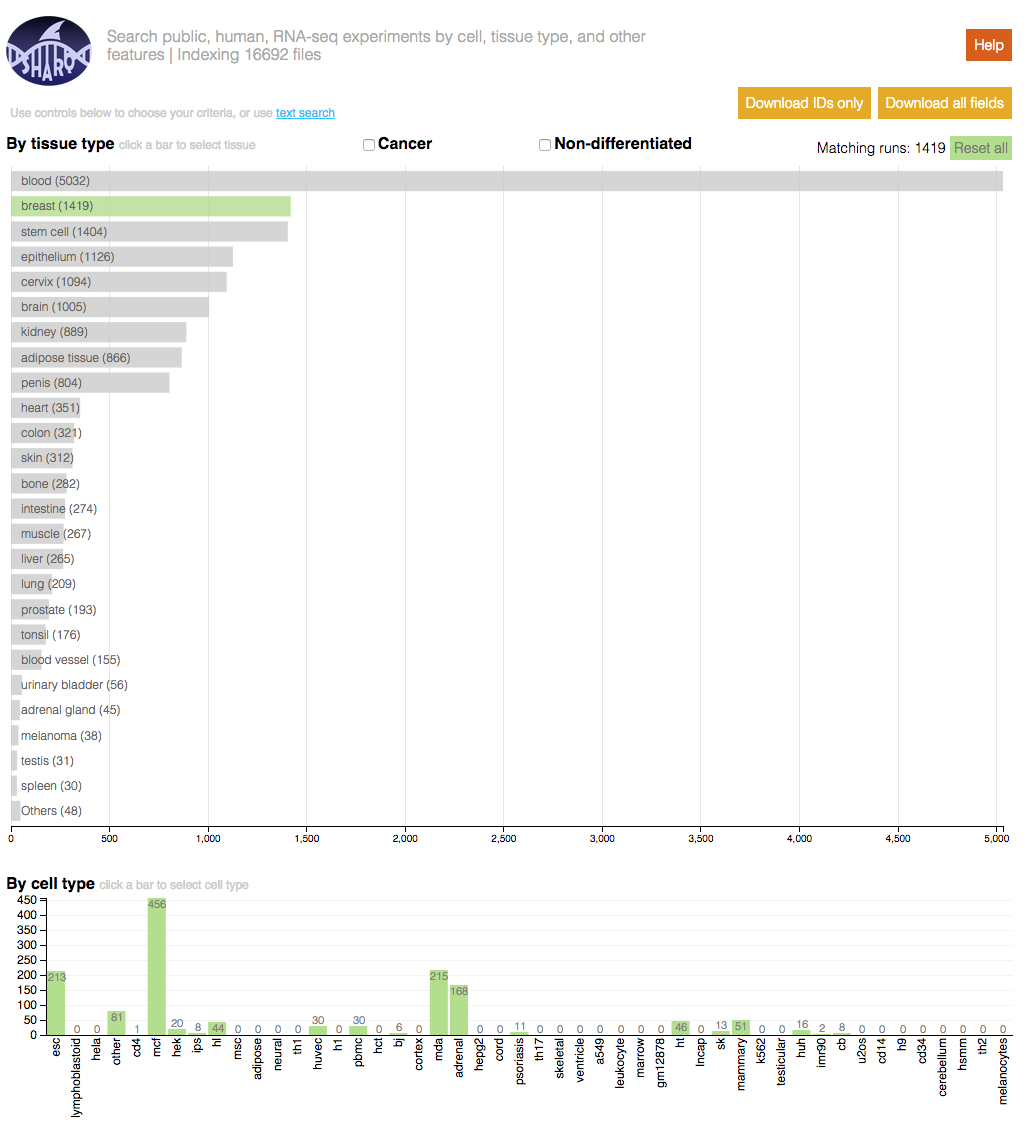
\includegraphics[width=\linewidth]{figures/sharq-ui.png}
%   \caption{\textbf{Overview of SHARQ interface.} The interface offers a variety of controls to search by multiple tissues, cell types, read length, or date of submission. Text search (not shown) scans through the PubMed abstracts and other text fields describing each sequencing run.}
%   \label{fig:sharq:interface}
% \end{figure}

% SHARQ is implemented as an lightweight web-based interactive tool using open source Javascript packages \texttt{crossfilter}~\cite{crossfilter} and \texttt{dc.js}~\cite{dcjs} (Figure~\ref{fig:sharq-ui}). It offers a way to quickly assess metadata for thousands of records and use visual cues to narrow the search down to a set of sequencing runs of interest. Users can start by selecting several tissue types, then refine the search by specifying  specific cell types or by restricting their search to runs that have a particular read length. Additionally, users can provide a date range that dictates the date of initial submission to SRA. As a special case, the user may choose to only focus on data associated with cancers or data associated with non-differentiated cells, since these samples may originate from any tissue. In addition to selecting parameters of interest, users may search across all text fields, such as study summaries, including tissue and cell type annotations. For example, searching for `blood' will bring select all sequencing runs that were annotated as coming from blood as all other runs that have a mention of `blood' in their annotations, title, abstracts, and summaries.\\

% Once users are satisfied with their query, they can download all matching sequencing run IDs in a single file for further processing --- these could be used, for example, for a batch download through SRA Toolkit \cite{leinonen2010sequence}. Alternatively, users can download full records for the matched runs that include FTP links for direct download.\\

% %%%%%%%%%%%%%%%%%%%%%%%%%%%%%%%%%%%%%%%%%%%%%%%%%%%%%%%%%%%%%%%%%%%%%%%%%%%%%%%
% \section{Discussion and conclusions}

% XXX





%%%%%%%%%%%%%%%%%%%%%%%%%%%%%%%%%%%%%%%%%%%%%%%%%%%%%%%%%%%%%%%%%%%%%%%%%%%%%%%
%%%%%%%%%%%%%%%%%%%%%%%%%%%%%%%%%%%%%%%%%%%%%%%%%%%%%%%%%%%%%%%%%%%%%%%%%%%%%%%
%%
%%
%% Map of jazz -- dynamic network vis
%%
%%
%%%%%%%%%%%%%%%%%%%%%%%%%%%%%%%%%%%%%%%%%%%%%%%%%%%%%%%%%%%%%%%%%%%%%%%%%%%%%%%
%%%%%%%%%%%%%%%%%%%%%%%%%%%%%%%%%%%%%%%%%%%%%%%%%%%%%%%%%%%%%%%%%%%%%%%%%%%%%%%
\chapter{Visualizing dynamic networks with context}
\label{chapter:mapofjazz}

Relationships between people, cooperation between genes in a cell, co-dependence of species within an ecosystem are just a few examples of interactions that are often modeled as a network, however, the fact that these networks are dynamic is often ignored. Dynamic networks may change in several ways: a gene that was not expressed in the previous time step may turn on; two proteins may form a complex under certain conditions (or two people become friends); the amount of a gene product may increase as a result of an activated pathway; the strength of a relationship between two people may grow over time. These changes are equivalent to node and edge gain and loss and directly affect network topology; the changes in the amount of a gene product or strength of a relationship are equivalent to property changes on the nodes and edges, but do not affect the graph structure itself.

The amount of information that changes between any two consecutive timepoints is often too great to comprehend even for small networks making visualization of such networks a challenging problem. We explore a setting in which the user focuses on a single node (e.g., a gene of interest) and its immediate neighborhood over time (ego-network). The main challenge is to maintain user's mental model of the ego-network between different time steps while allowing changes to propagate through the visualization. We model the amount of ``influence'' shared between the main node and its peripheral connections at any given time and develop an algorithm that assigns unique positions to the peripheral nodes according to the amount of shared influence. We suggest novel widgets to inform the user of general patterns of interaction between the main node and its neighbors.

In this chapter, we discuss a new system for exploring, in an intuitive and interactive way, a large compendium of collaboration data between jazz musicians. The system consists of an easy-to-use web application that marries an ego-network view of collaborations with an interactive timeline.  We develop a new measure of collaboration strength that is used to highlight strong and weak collaborations in the network view. The ego-network is arranged using a novel algorithm for ordering nodes that avoids occlusion even when the network is frequently changing. We build the system around a large, unique, hand-curated data set of recorded jazz collaborations. The ideas we develop in this chapter are applied to a social network, but can be easily extended to other types of dynamic networks, in particular, those where the numerical attributes on nodes and edges change over time. One such example is the gene co-expression network where genes control the expression of other genes in the cell.

The work discussed in this chapter was presented at SocialCom 2012~\cite{Filippova2012moj}. The system can be accessed at \url{http://mapofjazz.com/socialcom}.

%%%%%%%%%%%%%%%%%%%%%%%%%%%%%%%%%%%%%%%%%%%%%%%%%%%%%%%%%%%%%%%%%%%%%%%%%%%%%%%
\section{Background}

  Social networks such as those between collaborators or friends are an object of intense study. Often, such connections are assumed to be immutable and the networks are considered static. However, there are many social interactions that violate this assumption: work colleagues, neighbors, acquaintances, friends, and family may all change over the course of a person's lifetime. This is particularly true of jazz collaborations where band members frequently come together for only a single recording session, and where some musicians have played with over a thousand other artists over their decades-long careers. Understanding changes in connectivity on a scale of the whole network can provide an insight about the global change within the network, but has proven to be a difficult task for both algorithmic~\cite{Hopcroft2004, Palla2005c, Tantipathananandh2007, TangLiuZhna08} and visualization~\cite{BenderDeMoll2006, Rosvall2010,Yi2010} approaches. Changes may affect the profile of an individual node in a significant way, but these observations are lost in the sea of data when analyzing the network as a whole. The dynamism of jazz collaborations requires new approaches to visualize frequently changing networks.

  Apart from the topological changes, there may be other, more subtle variations in the characteristics of relationships over time.  Node or edge attributes may change, e.g.\@ the relationship between $A$ and $B$ may gradually change from an acquaintance to a close collaboration, or the ``importance'' of $A$'s immediate collaborators may grow, thus indirectly increasing the importance of $A$ itself.  Collectively, such changes may affect the profile of an individual in a significant way, but these observations are lost in the sea of data when analyzing the network as a whole. This, along with a traditional focus on the lives of individual musicians, leads to the desire to have a visualization that can be focused on subregions of the entire space of collaborations. It also leads to the need for techniques to quantify the strength of the relationships encoded in an evolving network and to show this information effectively through a visualization.

%%%%%%%%%%%%%%%%%%%%%%%%%%%%%%%%%%%%%%%%%%%%%%%%%%%%%%%%%%%%%%%%%%%%%%%%%%%%%%%
  \subsection{Jazz collaboration networks}

  The evolving community of jazz musicians is an example of a social network where personal connections are essential~\cite{Pinheiro2009}. In jazz, a highly collaborative art form, one person's individual style is shaped by constant experimentation and exchange of techniques and ideas with fellow musicians~\cite{Berliner1994}.  Every musician is part of a dense network of collaborators with many transient connections: a composer may arrange music for multiple bands simultaneously, band leaders may recruit new members to their bands and lose them to competition, or musicians' skills may improve to the point where they are featured as soloists and have a prominent place in the band. Study of recorded jazz collaborations can help identify influences on style, explain career success, and lead to a richer understanding of the progression of the jazz art form.

  The traditional means by which these collaborations are explored is via the compilation and study of discographies presented as lists and tables in either hard-copy books or in computerized databases~\cite{Timner2007,Albin}. These discographies list recording sessions, the roles each musician played in them, often songs and albums that were produced as a result, along with other information. They provide an extremely rich source of information from which to trace the collaborations of musicians. However, such a static and textual presentation is difficult to comb through and does not easily allow the user to comprehend the dynamics of changing collaborations. While changes in band membership are easily traceable, it is hard to assess the overall contribution of a band member over time unless the historians are intimately familiar with the band's history. A system for exploring jazz collaborations that makes large discography data more approachable is needed.

  

%%%%%%%%%%%%%%%%%%%%%%%%%%%%%%%%%%%%%%%%%%%%%%%%%%%%%%%%%%%%%%%%%%%%%%%%%%%%%%%
  \subsection{Dynamic network visualization}

  There are two main approaches to visualizing time-varying networks: to show animations by constantly recomputing layouts at every time step~\cite{Yee2001} and to compare static snapshots of a network at several distinct time points. For either approach, the objective is to highlight the differences between the network views at different time steps.

  Brandes and Corman~\cite{Brandes2003a} stack network snapshots on top of each other in 3D where the nodes with the same labels are connected by vertical columns. The graph is laid out using a spring-embedded algorithm, and each slice shows only the nodes and edges present at that time point. Yim, Shaw, and Bartram~\cite{Yim2009} show a snapshot of a network in its early state and indicate changes in node positions with red arrows leading to complicated and cluttered displays. Diehl and G\"{o}rg~\cite{Diehl2002} place the two network snapshots side by side and propose three algorithms that minimize dissimilarities between the two representations. A recent study by Khurana et al.~\cite{Khurana2011} presents an extension to NodeXL~\cite{Bonsignore2009} that aggregates the snapshots of a network at two different time points into a single view. The edges are colored based on the time interval at which they existed. Additionally, NodeXL plots the values of several common graph properties such as node and edge counts as they change over time between the two time points. An approach by Yi et al.~\cite{Yi2010} combines a small multiples display (a histogram showing node degree over time) and a matrix representation of a network into a single view.

  Graph layout for the animations may be fixed or constantly updating at each time step. Moody et al.~\cite{Moody2005} keep the node positions fixed and allow the edges to appear and disappear as the time progresses in their \emph{flip-book} animations. Yee and colleagues~\cite{Yee2001} allow the nodes to move between the concentric circles along a smooth tangential trajectory.

  While these approaches are able to highlight the topological changes, they all make an assumption that node and edge attributes (such as edge length) are either absent or remain static over time.

  % related work: circular layouts

%%%%%%%%%%%%%%%%%%%%%%%%%%%%%%%%%%%%%%%%%%%%%%%%%%%%%%%%%%%%%%%%%%%%%%%%%%%%%%%
  \subsection{Circular and ego-network layouts}

  Circular layouts have been used for organizing trees by placing the root in the center and assigning the child nodes to concentric circles with increasing radii~\cite{North1997}, with nodes at the same level of a tree assigned to the same circle. Six et al.~\cite{Six1999} extended the technique to work for more general graphs by connecting multiple circular structures. Yee and colleagues~\cite{Yee2001} have developed the technique further to support nodes of different sizes (where node size is proportional to some node attribute). They adapted their layout to handle dynamic graphs by showing animations of nodes traveling on a smooth trajectory from old locations to the new ones.

  Wang, Shi, and Wen~\cite{Wang2011a} experiment with a dynamic ego-network design where the central node and all of its connections are shown at the same time. The main node has several copies with each one representing the node at a specific point in time and linked only to those nodes with which it was associated during that period. This approach is not feasible if the central node has many collaborators over his or her career. Gansner and Koren~\cite{Gansner2006} develop heuristics that order nodes on a circle's periphery in a way that minimizes the edge crossovers and reroutes some of the links to go outside the circle's circumference. These authors suggest edge bundling for the links inside the circle to reduce clutter further. Their work does not consider dynamically changing links.

%%%%%%%%%%%%%%%%%%%%%%%%%%%%%%%%%%%%%%%%%%%%%%%%%%%%%%%%%%%%%%%%%%%%%%%%%%%%%%%
  % related work: collaboration networks
  \subsection{Artist collaboration networks}

  Artist collaboration networks have received their fair share of attention in social network analysis. The data on interactions among musicians is available in some databases~\cite{Gleiser2003,Pattuelli2012}, has been collected through surveys~\cite{Heckathorn2001a}, or assembled manually by processing the tapes of interviews with the artists~\cite{Pattuelli2011}. Due to difficulties in data collection, these sources cover only a few artists and lack temporal information about their collaborations. For example, Gleiser and colleagues~\cite{Gleiser2003} base their analysis on 198 bands that were active in 1912-1940. Heckathorn and Jeffri's survey reached out to 110 musicians in New Orleans, 264 in New York, and 300 in San Franscisco~\cite{Heckathorn2001a}, a small fraction of the estimated 33,000 jazz musicians living in New York.

  Examples of applications supporting exploration of such networks are few. An online Classical Music Navigator~\cite{Smith1999} helps users expand their musical interests by suggesting composers who influenced or were influenced by a composer the users initially searched for. The Navigator offers a simple text and link interface. A visualization of Last.fm data~\cite{Bieh-Zimmert2011} allows one to compare two artists and their musical associations, but does not provide any intuition about collaborations between the two artists.

  In this paper, we propose a way to quantify the strength of collaboration between two actors in the network based on the frequency and timing of the events in which they have both participated. We provide a visualization system that displays much of the data available in large discographies. In this network, nodes represent artists and edges connect artists who participated in the same recording session at some time. We visualize creative partnerships between musicians using an interactive egocentric network view that allows users to focus on an individual and observe large and small scale changes in collaborations (Figure~\ref{fig:moj:overview}). We couple this network view with an interactive timeline that allows the user to see how the strength of ties changed over time. We also introduce a novel algorithm that arranges collaborator nodes around the central musician in a way that minimizes node occlusion and variation in node positions as the network view changes over time. This helps the users to maintain their mental map of evolving collaborations. We demonstrate the utility of this approach on an extensive hand-curated collection of jazz collaborations spanning almost a hundred years.

%%%%%%%%%%%%%%%%%%%%%%%%%%%%%%%%%%%%%%%%%%%%%%%%%%%%%%%%%%%%%%%%%%%%%%%%%%%%%%%
\section{Dynamic network data}

  % Describe the process of entering, cleaning, improving, expanding,
  % cross-referencing.

  The Map of Jazz uses data that have been collected over the course of more than twenty years of discographical research, with additional content subsequently added in targeted batches. The data come from a myriad of sources: from general and artist discographies to specialist journals, magazines, and newsletters to biographical and historical monographic literature and many more. In almost every case, a single entry is a collection of data from multiple sources because no one source covers every aspect of the recording session. The sessions cover a period of time from the early 1920s to the present day.

  While there have been other attempts at digitizing discographical information, these used closed, proprietary systems that lacked both the ability to export and import or edit the information, and ultimately were unable to satisfy the information needs of serious researchers. The data used by the Map of Jazz were collected and stored using the open-source discographical software BRIAN~\cite{Albin}, named so for the English discographer Brian Rust who perfected the session-based format for print discographies~\cite{Rust1980,Rust2002}. BRIAN's support for data export and import allowed for multiple users to contribute to the project and amounted to a large number of cataloged recording sessions. The Map of Jazz is the first project to use large amounts of BRIAN data outside of the application itself.

  At the heart of BRIAN is the conceptual idea that the session is the primary entity, unlike many other databases designed to store sound recordings information. Sessions are events that have defined locations, both chronologically and geographically. Out of the many layers of details available in BRIAN, the Map of Jazz uses the top-level data on the sessions and musicians who performed during them, thus shifting the focus to the interpersonal relationships between the artists. The attribute for the main musical instrument helps to distinguish Bill Evans the saxophonist from Bill Evans the pianist; it also records what instrument each performer played.
  %
  % Top 5 guys by the number of collaborators
  %
  \begin{table}
    \centering
    \begin{tabular}{l  r}
    \toprule
    Name & Degree \\
    \midrule
    Slide Hampton & 1230\\
    Kenny Barron & 1090\\
    Ron Carter & 785\\
    Michael P. Mossman & 692\\
    Freddie Hubbard & 691\\
    \bottomrule
    \end{tabular}
    \caption{\textbf{Top 5 musicians with the highest number of collaborations.} Slide
    Hampton was a prolific composer who has provided arrangements for multiple
    bands, hence his interaction surpasses that of many famous band leaders.}
    \label{tab:high_degree}
  \end{table}
  %

  % Data statistics.

  \begin{figure}[t]
    \centering
    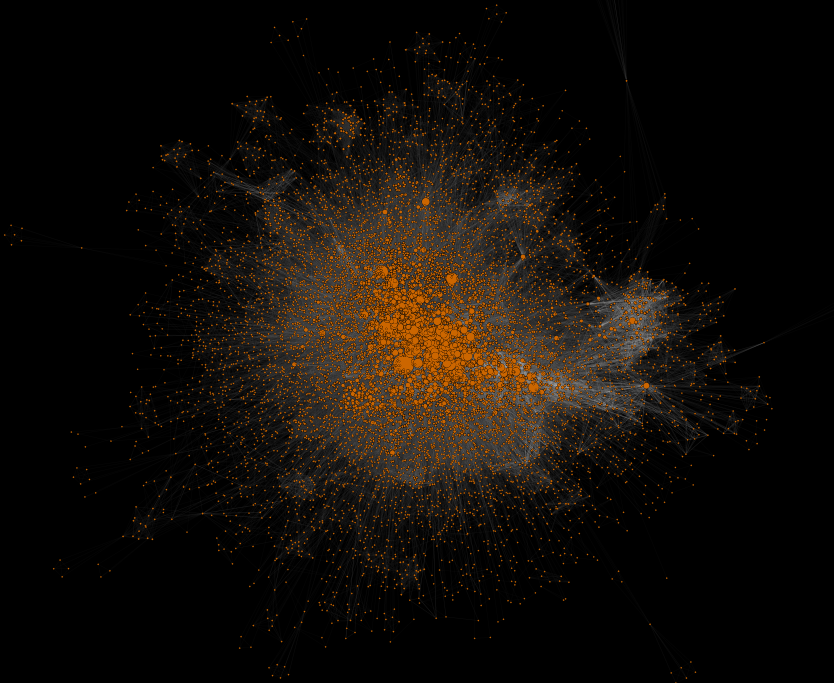
\includegraphics[width=\linewidth]{figures/full_network_cropped.png}
    \caption{\textbf{Map of Jazz network of collaborations} visualized with Cytoscape~\cite{Cytoscape}. Individual nodes represent jazz musicians, node size corresponds to node degree, and the opacity of the edges between nodes corresponds to the frequency of collaboration over time.}
    \label{fig:moj:fullnetwork}
  \end{figure}



  At the time of publication, the database contained information on 11824 musicians and a total of 13873 recording sessions (see Figure~\ref{fig:moj:fullnetwork} for an overview of the collaboration graph). The average number of people per recording session was 7.39 with the smallest sessions having just one performer, and the largest session having 72 people (not including the members of symphony orchestras). Network diameter (the longest among all shortest paths between all pairs of vertices) was equal to 8, and the average (\emph{characteristic}) shortest path was equal to 3.24. As with many social networks, very few musicians have a high number of connections, with an overall average node degree of 33.68 (see Figure~\ref{tab:high_degree} for the top 5 artists by degree). However, the network does not pass the test for scale-freeness according to the test developed by Clauset et al.~\cite{Clauset2009b} suggesting that the network has evolved by processes other than the well-studied ``rich get richer"mechanism.



%%%%%%%%%%%%%%%%%%%%%%%%%%%%%%%%%%%%%%%%%%%%%%%%%%%%%%%%%%%%%%%%%%%%%%%%%%%%%%%
\section{Interface design}


  The Map of Jazz focuses on the dynamics within the collaboration networks of individual musicians. An egocentric network layout (Figure~\ref{fig:moj:overview}) is coupled with an interactive timeline that allows users to navigate through various time periods and observe gradual changes in the person's collaboration network. The timeline is augmented with aggregate statistics, such as the number of people per sessions, to aid in navigation through time. In the network view, nodes representing collaborators are arranged around the central node in a manner that preserves nodes' relative positions across time and shows the relative strength of a tie between the main musician and his or her collaborator. Nodes and edges used in the traditional node-link network representation are extended to display the change in attribute values over time. Finally, the interactions between the currently displayed main musician's collaborators can be explored on demand by highlighting a node of interest which reveals its connections to other nodes in the neighborhood. The central artist can be selected by double-clicking on a performer's node or by entering a musician's name in a search box. To help users pick a starting point, the Map of Jazz offers a dropdown with 21 hand-picked sessions that stand out in jazz history.


  \begin{figure}[tb!]
    \centering
    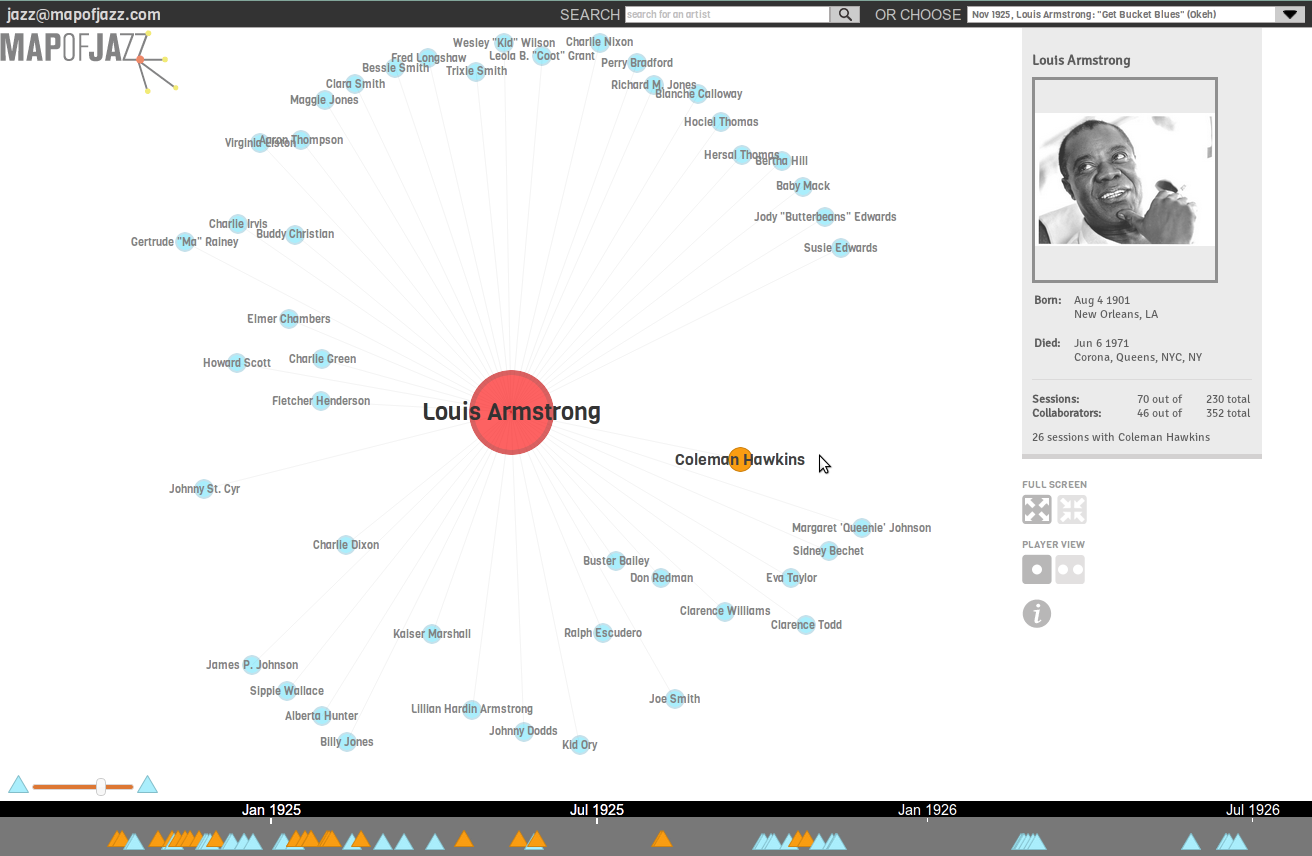
\includegraphics[width=\linewidth]{figures/moj_overview.png}
    \caption{\textbf{Overview of the Map of Jazz web application.}}
    \label{fig:moj:overview}
  \end{figure}


  %%%%%%%%%%%%%%%%%%%%%%%%%%%%%%%%%%%%%%%%%%%%%%%%%%%%%%%%%%%%%%%%%%%%%%%%%%%%%%%%
  %
  % Visual: timeline
  %
  %%%%%%%%%%%%%%%%%%%%%%%%%%%%%%%%%%%%%%%%%%%%%%%%%%%%%%%%%%%%%%%%%%%%%%%%%%%%%%%%

  \subsection{Timeline}

  Users may navigate the extensive Map of Jazz timeline by dragging it with a
  mouse. They may also zoom in on a particular period of the musician's life or
  zoom out to get an overview of the artist's career. Every time the users
  interact with the timeline, the ego-network is updated to present an accurate
  snapshot for the selected time period.

  \textbf{Sessions.} The triangles on the timeline represent recording sessions (Figure~\ref{fig:moj:timeline}). When users hover over the triangle with a mouse, the session and the collaborators who recorded for that session are highlighted in yellow. Users may click on a session to select all the participating collaborators and the session itself, and vice versa. A tooltip that appears above the triangle icon summarizes the information about the session: the date, location, and a list of participating musicians along with their primary skill (an instrument they played, e.g.~alto saxophone, or a role they took, e.g.~band leader, during a session).

  When the date of birth and/or death are available, the span of time from birth to death (or to the present day) is colored in a lighter shade of gray to indicate the span of the musician's life.


  %
  \begin{figure}[ht]
    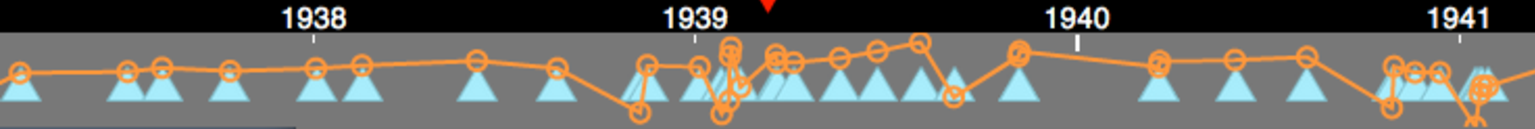
\includegraphics[width=\linewidth]{figures/timeline}
    \caption{\textbf{A timeline augmented with a session similarity graph.} Triangles represent the individual recording sessions. Most sessions on the timeline have a high pairwise similarity indicating that session memberships changed only slightly.}
    \label{fig:moj:timeline}
  \end{figure}
  %

  
  \textbf{Augmented timeline.} To aid users in focusing on a specific time period of interest, the Map of Jazz offers several basic metrics to be overlaid on top of the timeline. These include: 
  %
  \begin{itemize}
    \item the number of collaborators per session
    \item the number of unique musicians the person collaborated with up to this date,
    \item the Jaccard similarity between the members of the current session and the previous session.
  \end{itemize}
  %
  The number of collaborators and the speed at which a person attracts new collaborators have been shown to be significant in scientific~\cite{Petersen2012} and jazz~\cite{Pinheiro2009} collaborations, while the session size may explain the mechanism of acquiring new collaborators (i.e. switching between bands versus playing with the same band).


  %%%%%%%%%%%%%%%%%%%%%%%%%%%%%%%%%%%%%%%%%%%%%%%%%%%%%%%%%%%%%%%%%%%%%%%%%%%%%
  %
  % Implementation: influence function
  %
  %%%%%%%%%%%%%%%%%%%%%%%%%%%%%%%%%%%%%%%%%%%%%%%%%%%%%%%%%%%%%%%%%%%%%%%%%%%%%%

  \subsection{Measure of collaboration strength}

  The notion of mutual influence between any two musicians lies at the heart of the Map of Jazz. To quantify the strength of the relationship between any pair of musicians, we make an assumption that the recording sessions are not spontaneous events, but rather a result of previous undocumented collaboration (e.g. concerts and rehearsals). Consequently, the professional relationship between the musicians is not likely to start right before a session nor to stop immediately after recording it, but rather to grow before the session and wane gradually over time. The collaboration is strongest around the time of a recording session and is increased even more if the musicians record several sessions over a short period of time. With these assumptions in mind, we define a function of \emph{collaboration strength} that takes into account the frequency and proximity in time of the collaborations between the two musicians:
  %
  \begin{equation}\label{eqn:influence}
  %
  g(t; S, \sigma) = \alpha_\sigma \sum_{s \in S} e^{-\beta_\sigma(t_s-t)^2 },
  %
  \end{equation}
  %
  where $S$ is the set of all sessions the two musicians shared, $t$ is a point in time for which we want to evaluate the collaboration strength (i.e.\@ the center of the timeline), and $t_s$ is the date for a specific session $s$. To make the decay of the collaboration strength smooth, we model it as a normal distribution with $\alpha_\sigma = 4/(\sigma^2\sqrt{2\pi})$ and $\beta_\sigma = 1/(2\sigma^2)$. %
  The function~\eqref{eqn:influence} is similar to a kernel density estimator for normally distributed values, where choosing the bandwidth for the kernel is a known hard problem. To make the function smooth, we take an affine combination of two functions:
  %
  \begin{equation}\label{eqn:influence2}
  %
  f(t; S) = \delta g(t; S, \sigma_1) + (1-\delta)g(t; S, \sigma_2),
  %
  \end{equation}
  %
  with $\sigma_1 = 1$, $\sigma_2 = 3$, and $\delta=0.9$. The resulting function assigns more impact to the interactions that were closer to $t$ in time rather than assign an equal weight to all interactions no matter how long ago, or how far in the future, they occurred (Figure~\ref{fig:moj:infl_func}).

  %TODO: Unlike the function used in~\cite{Palla2005c}), we take into account both
  %the past and the future collaboration events.

  \begin{figure}[ht]
    \centering
    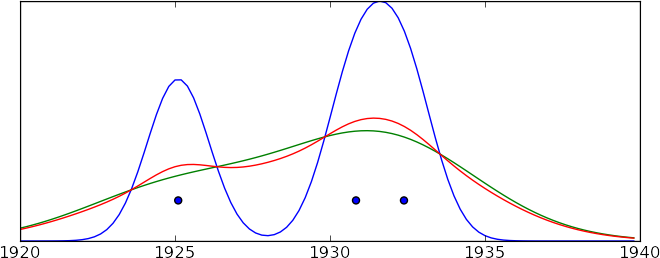
\includegraphics[width=0.6\linewidth]{figures/influence_plot.png}
    \caption{\textbf{The collaboration strength function} (red) is a combination of two functions: one for which  the value grows fast as $t$ gets closer to the session (blue) and another one for which the change in value is much smoother (green). Here, two hypothetical musicians played together in 1925, 1930, and 1932 (blue dots). Their relationship is strongest when several sessions occur within a short period of time such as in 1930--1932. The collaboration strength drops slightly between 1925 and 1930 and declines rapidly after the last session in 1932.}
    \label{fig:moj:infl_func}
  \end{figure}


  %%%%%%%%%%%%%%%%%%%%%%%%%%%%%%%%%%%%%%%%%%%%%%%%%%%%%%%%%%%%%%%%%%%%%%%%%%%%%%%%
  %
  % Visual design: egonetwork
  %
  %%%%%%%%%%%%%%%%%%%%%%%%%%%%%%%%%%%%%%%%%%%%%%%%%%%%%%%%%%%%%%%%%%%%%%%%%%%%%%%%
  \subsection{Egocentric network view}

  An egocentric view allows the user to track the fluctuating interactions between a given musician and his or her peers over time. Using the timeline, users may select a time range of interest and focus on the collaborations between the main musician and his or her collaborators within that period. Only the collaborators that were involved in sessions that occurred during that time range will be shown. For every collaborator $v$, we compute the collaboration strength between the center musician $u$ and $v$ where $S$, the set of sessions considered in the collaboration strength function, equals the sessions that are currently visible on the timeline. The length of an edge connecting $u$ and $v$ is inversely proportional to the strength of the tie shared by the two artists, as measured by the collaboration strength function~\eqref{eqn:influence}. This causes the collaborators who record with the main musician $u$ often or have recorded with him or her recently to be placed closer to the center, while musicians who record with $u$ rarely or have only recorded with $u$ a long time ago are placed on the periphery (Figure~\ref{fig:moj:overview}).

  As users drag the timeline, the collaborators' nodes may move closer to the center or may drift away to the periphery as the set of sessions that is displayed changes. Nodes disappear from view when they are no longer involved in any session that is visible on the timeline, and new nodes appear when sessions containing them come into view on the timeline. To minimize the cognitive load on the users, the Map of Jazz preserves the angular positions for every collaborator node within the ego-network formed by a particular main musician. For every musician $u$, we assign a unique angular sector to every collaborator $v$ who has ever recorded with $u$ (Figure~\ref{fig:moj:ordering}). Their trajectory, a straight line connected to the center, can be easily traced as collaborator nodes move to or from the center.

  If care is not taken with the assignments of nodes to angular sectors, collaborators may crowd near the center if the main musician consistently played with the same set of people (i.e.\@ their band). To avoid this, we propose an ordering algorithm in Section~\ref{sec:moj:ordering} to arrange the collaborator nodes in a way that assigns dissimilar angles to collaborators with which the center node has had similar patterns of collaboration.

  %TODO: highlight nodes that just showed up OR have a session with the main guy
  %withing $\epsilon$ distance of $t_{center}$

  %[XXX (move to ego-net) Users control the animation between two different states
  %by zooming in and out of the timeline and by dragging the timeline left or
  %right. These actions change the $t_c$ time thus causing layout to update.]

  %%%%%%%%%%%%%%%%%%%%%%%%%%%%%%%%%%%%%%%%%%%%%%%%%%%%%%%%%%%%%%%%%%%%%%%%%%%%%%%%
  %
  % Implementation: ordering collaborators
  %
  %%%%%%%%%%%%%%%%%%%%%%%%%%%%%%%%%%%%%%%%%%%%%%%%%%%%%%%%%%%%%%%%%%%%%%%%%%%%%%%%

  \subsection{Ordering collaborators in a circle}
  \label{sec:moj:ordering}

  % TODO: Test how heterogeneous/homogeneous interaction are over time for most
  %people? High degree ppl? Low degree ppl?

  The Map of Jazz maintains the same angular node positions across every time
  period, allowing easier comparison of the network at different time points. As
  users navigate the timeline, new nodes may show up on the map, but they will
  never change the angular position of the nodes already on screen, thus
  preserving the users' mental map of the ego-network.

  The permanent angular node positions also help alleviate another problem common
  to graph drawing: node occlusion. More often than not, jazz musicians have a
  band, or several bands, with which they play and record on a regular basis. In
  this case, every person in the band would share a strong tie with the musician
  in question. The Map's circular layout would try to place all such frequent
  collaborators near the center, causing the nodes and labels to occlude each
  other.

  To minimize such occlusions, we identify groups of people that are likely to be
  at the same distance from the central node at the same time. To find the groups,
  we first sample the collaboration strength function values between the main
  musician $u$ and each one of its collaborators $v$:
  %
  \begin{equation}\label{eqn:sample}
  %
    x_{u, v} = (f(t_1;S), f(t_2;S), \ldots, f(t_{1000};S)),
  %
  \end{equation}
  %
  where $t_i$ are equally spaced time points in the range $[t_\textrm{min}, t_\textrm{max}]$ with $t_\textrm{min}$ equal to the date of $u$'s earliest session and $t_\textrm{max}$ equal to the date of $u$'s last recording session. In~\eqref{eqn:sample}, $S$ is the set of all the sessions in which the central node $u$ participated. Next, we construct a pairwise similarity matrix for all $u$'s, $M_u = \left(m^u_{i,j}\right)$, where $m^u_{i, j}$ is the cosine similarity between vectors $x_{u,v_i}$ and $x_{u,v_j}$. To make it easier for the clustering algorithm to find groups in this matrix, we set every $m^u_{i,j} < 0.9$ to $0$. The resulting sparse matrix $M'_u$ is taken as a weighted adjacency matrix of a graph $G_u$. We run the Louvaine clustering algorithm~\cite{Blondel2008}, which attempts to find clusters maximizing modularity~\cite{newman06}, on $G_u$ to identify groups of musicians for whom the $x_{u, v_i}$ vectors were similar.

  Performers in the same cluster interact with the main performer in a similar fashion. To spread them out, we assign them sectors of the circle that are far from each other.
  %
  \begin{figure}[ht]
    \centering
    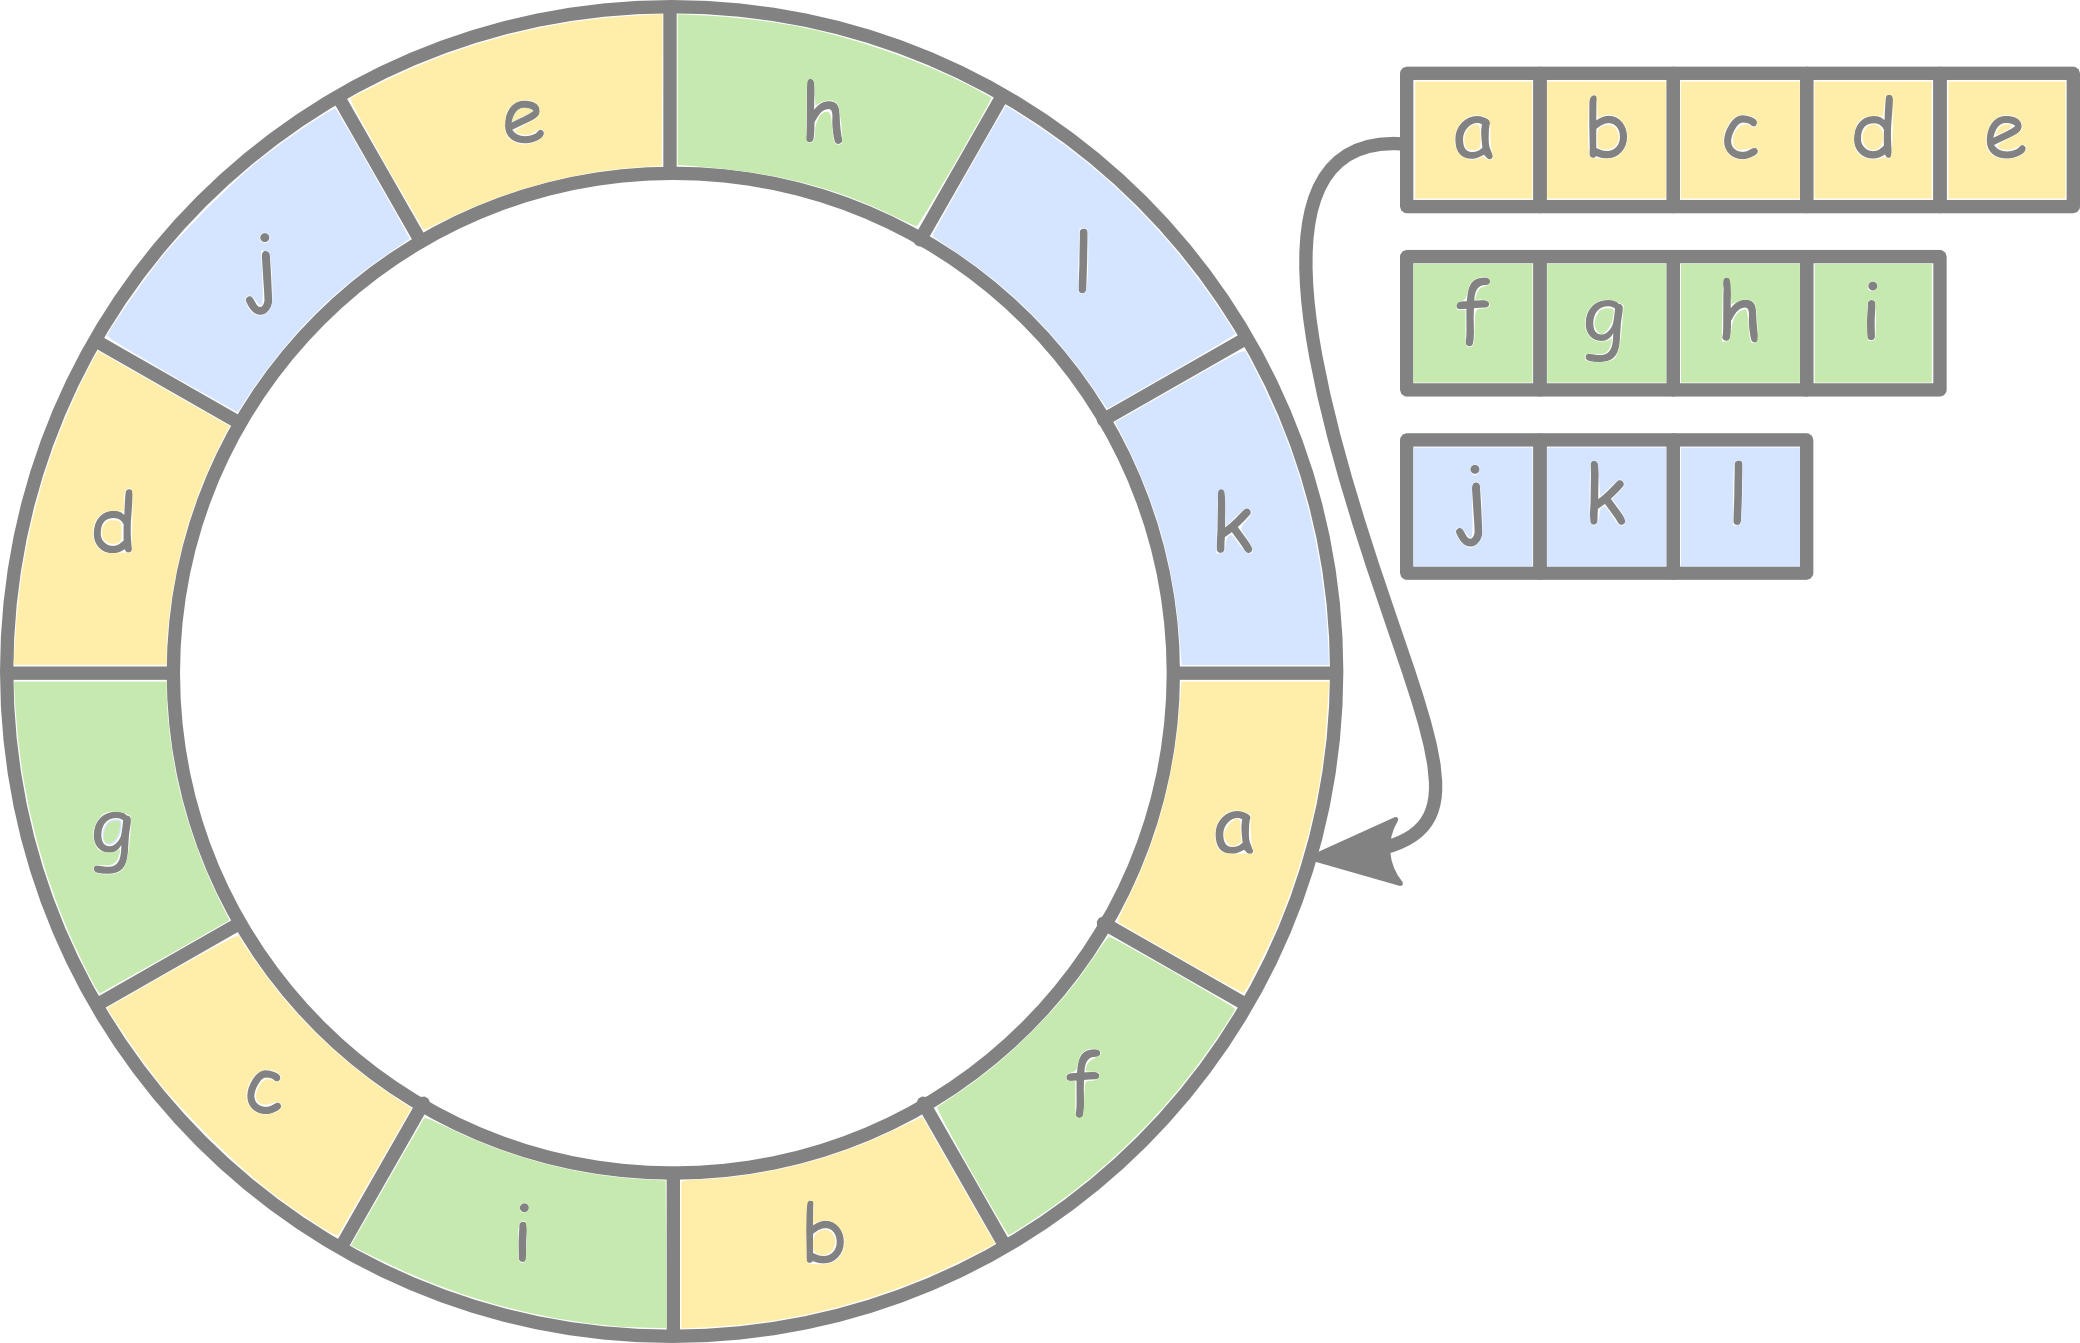
\includegraphics[width=0.6\linewidth]{figures/ordering}
    \caption{\textbf{Assigning angular positions for the nodes.} Starting with the largest cluster, performers from the same cluster get assigned sectors of the circle that are far from each other. Here, \emph{a} is assigned to the $1^\textrm{st}$ sector, \emph{b} is $\left\lfloor \frac{12}{5} \right\rfloor = 2$ sectors away, and so on.}
    \label{fig:moj:ordering}
  \end{figure}
  %
  To assign all $N$ collaborators to their angular positions, we iterate through the clusters in order of decreasing size.  For each cluster $C$, we assign a node in $C$ to the first empty sector and continue assigning $v \in C$ to empty sectors evenly around the circle at intervals of $\left\lfloor\frac{N}{|C|}\right\rfloor$ sectors.  If at any time the target sector is not empty, we search linearly clockwise for the next available sector and continue assigning the remaining nodes in $C$ starting from that sector (Figure~\ref{fig:moj:ordering}). This heuristic --- similar to linear reprobing in a hash table --- attempts to ensure that the nodes belonging to the same cluster are spread out around the circle at equal intervals.

  %%%%%%%%%%%%%%%%%%%%%%%%%%%%%%%%%%%%%%%%%%%%%%%%%%%%%%%%%%%%%%%%%%%%%%%%%%%%%%%%
  %
  % Visual: Node glyphs
  %
  %%%%%%%%%%%%%%%%%%%%%%%%%%%%%%%%%%%%%%%%%%%%%%%%%%%%%%%%%%%%%%%%%%%%%%%%%%%%%%%%

  \subsection{Node and edge glyphs}

  A static snapshot of a collaboration ego-network may be misleading due to the fact
  that the past and future collaborations between the central and peripheral nodes
  are not visible. A collaboration that flourished previously may be represented
  by a single recording session in the selected time period and could be
  indistinguishable from many sporadic one-time collaborations. Likewise, an
  ego-network does not provide enough detail about the level of activity for the
  nodes other than the central node based on the edge length alone. Questions such
  as: did the musicians represented by these nodes record often? How many sessions
  did they record overall within this time period? Will they continue recording
  actively? To answer these kinds of questions, we replace the standard graph
  nodes and links with more information-dense glyphs.

  We use node glyphs to represent the collaborator's activity overall
  (i.e. sessions recorded, not necessarily with the main musician), and reserve
  the edge glyphs to represent collaborations between the main musician and the
  collaborator. The node glyphs, therefore, encode the musician's overall artistic
  output while the edges connecting it to the main musician quantify the strength
  of the tie between them.

  \begin{figure}[ht]
    \centering
    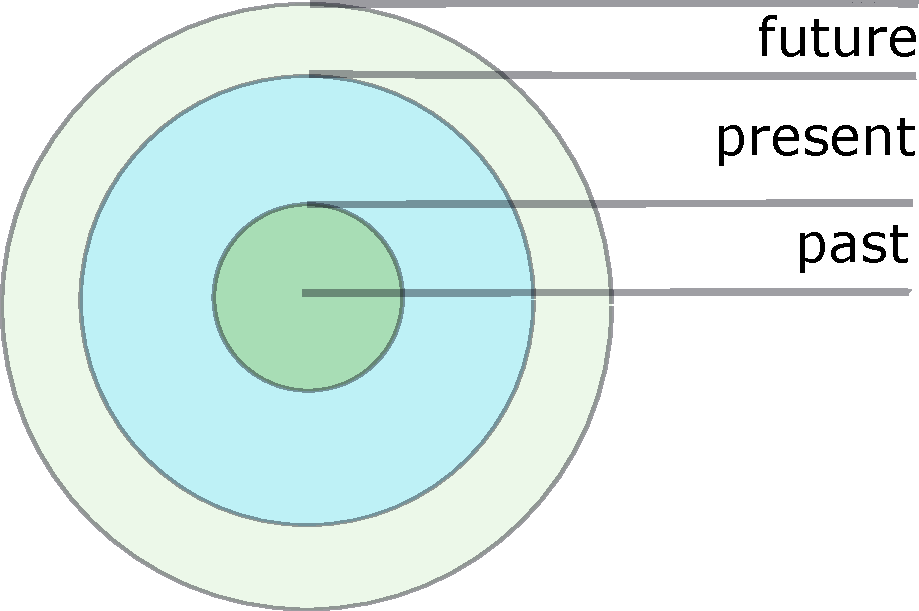
\includegraphics[height=100px]{figures/node-glyph}
    \caption{\textbf{Node glyph.} The radius of the inner-most circle of the node glyph is a function of the number of times the musician played in \emph{some} session in the past. We use square root as the function here since it results in noticeable differences for small values and does not unexpectedly explode in size for high values. The middle circle (blue) represents the number of sessions the musician played with the main musician within the current time frame. The radius of the outer largest circle encodes the total number of sessions the musician played throughout his/her career with or without the main musician.}
    \label{fig:moj:node_glyphs}
  \end{figure}

  Node glyphs (Figure~\ref{fig:moj:node_glyphs}) consist of three concentric circles.
  The inner circle's radius is proportional to the square root of the count of
  sessions this musician played in the past, i.e. before the sessions currently
  visible on the timeline. The second circle's radius represents the square root
  of  the number of sessions from both the past and currently visible on the
  timeline in which that collaborator recorded. The radius of the outer circle is
  proportional to the square root of the total number of sessions the musician has
  recorded throughout their life. As users navigate the timeline in the direction
  of the future, more sessions would transfer to the ``past'' circle, increasing
  the radius of the inner-most circle. The radius of the circle representing the
  ``past+present'' may fluctuate depending on the number of sessions currently
  visible on the timeline. The radius of the outer circle, i.e. the square root of
  a total number of sessions recorded, does not change.

  Edge glyphs encode information about the overall count of recording sessions in which both the main musician and the collaborator participated (Figure~\ref{fig:moj:edge_glyphs} and~\ref{fig:moj:duke-ell}). Edges are colored in varying shades of gray with the inner edge representing collaborations in the ``past'' and its thickness proportional to the square root of the number of sessions he or she shared with the main musician in the past. The thickness of the middle part is a function of the square root of the number of sessions for that collaborator currently visible on the timeline. Finally, the total edge thickness represents the number of sessions the two musicians played together overall. As users interact with the timeline, the thickness of the inner edges may change depending on the number of shared sessions in the past or currently visible on the timeline; however, the total thickness of an edge would not change.

  \begin{figure}[ht]
    \centering
    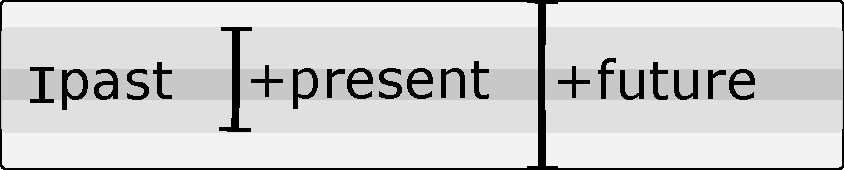
\includegraphics[width=0.5\linewidth]{figures/edge-glyph}
    \caption{\textbf{Edge glyph.} The thickness of the inner-most inset in the edge glyph
  is proportional to the number of sessions the main musician and their
  collaborator played in the past, and the thickness of the "present" inset
  corresponds to the count of sessions in the past and present. The total edge
  thickness represents the number of sessions the two musicians played together
  overall.}
    \label{fig:moj:edge_glyphs}
  \end{figure}

  Various combinations of node and edge thicknesses should alert the users to different modes of collaboration. A combination of a large peripheral node and a narrow edge connecting it to the center indicates that while the collaborator has played many sessions overall, they played very few with the main musician (for example, Don Redman in Figure~\ref{fig:moj:duke-ell}). Further, if the node's inner ``past'' circle is large, such combination then indicates that the collaborator is an established musician who is sharing their skills with the up and coming musician at the center of the ego-network. On the contrary, if the inner ``past'' circle is small and the majority of sessions are in the ``future'', such behavior may indicate that the collaborator has joined the main musician briefly and later went on to form an active career of their own. A case where both the node and the edge are thick indicates that the two musicians have recorded many sessions together and, therefore, share a strong tie.

  %%%%%%%%%%%%%%%%%%%%%%%%%%%%%%%%%%%%%%%%%%%%%%%%%%%%%%%%%%%%%%%%%%%%%%%%%%%%%%%%
  %
  % Visual: hops
  %
  %%%%%%%%%%%%%%%%%%%%%%%%%%%%%%%%%%%%%%%%%%%%%%%%%%%%%%%%%%%%%%%%%%%%%%%%%%%%%%%%

  \subsection{Exploring collaborators' connectivity}

  An ego-network allows users to focus on the dynamics of a few collaborations at the expense of hiding all other topological information. Knowing which, if any, peripheral nodes collaborate with each other helps to understand the communities that form in the immediate neighborhood of the main musician. The Map of Jazz provides such details on demand: when users hover over a collaborator's node $v$, the Map renders additional edges that connect $v$ to the collaborators it shares with the central node (Figure~\ref{fig:moj:young}). The thickness of the edges corresponds to the number of sessions the two musicians played in the past (including those they played with the main musician). When the edges connecting the main node and the performers on the periphery are thin indicating few collaborations, it would be noteworthy to see thick edges between those performers. Such a situation would imply that those artists form a strong community, or a band, outside of the main musician's neighborhood.

  %%%%%%%%%%%%%%%%%%%%%%%%%%%%%%%%%%%%%%%%%%%%%%%%%%%%%%%%%%%%%%%%%%%%%%%%%%%%%%%%
  %
  % User study
  %
  %%%%%%%%%%%%%%%%%%%%%%%%%%%%%%%%%%%%%%%%%%%%%%%%%%%%%%%%%%%%%%%%%%%%%%%%%%%%%%%%

  %\section{Evaluation}
\section{Example analysis with the Map of Jazz}

  \textbf{Duke Ellington}'s career spanned more than half a century from the early twenties to his death in 1974. The first record on the Map's timeline dates back to July of 1923 with Ellington playing piano and Elmer Snowden as the band leader --- Ellington was yet to form his own band. Ellington's egonet for the period of 1923--1928 has several prominent performer nodes: Harry Carney, Otto Hardwick, Sonny Greer, Fred Guy,  Barney Bigard, Joe Nanton, and Wellman Braud (see Figure~\ref{fig:moj:duke-ell}). The size of Harry Carney's node, for example, indicates that he participated in a significant number of recording sessions throughout his career (1487 sessions), and the thickness of the edge connecting him to Duke Ellington reveals that most of those sessions were recorded with Ellington (1480 sessions). The same holds for others in the list above: their careers were tightly knit with Ellington's.


  \begin{figure}[tb!]
    \centering
    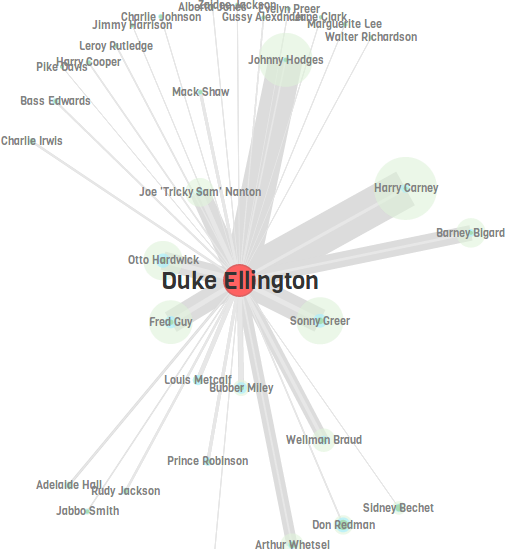
\includegraphics[width=0.7\linewidth]{figures/duke-ellington-1925-1928}
    \caption{\textbf{Ego network.} Duke Ellington's ego-network during 1925--1928. His prominent collaborators, Otto Hardwick, Fred Guy, Sonny Greer, Johnny Hodges, and Harry Carney, can be easily identified by the thick edges.}
    \label{fig:moj:duke-ell}
  \end{figure}

  % overview of timeline

  From the details window, it is clear that Duke Ellington had a very productive career: over the course of his life he participated in more than 1740 sessions with 600 musicians. If the user zooms out on the timeline, it becomes evident how densely packed Ellington's recording sessions were, with the last right before his death. The pairwise session similarities that are visible on the timeline and the average pairwise similarity of 0.60 suggest that Ellington played with a core group of close collaborators who would replace one another over the years, but the band membership never changed all at once. Switching to the graph of session sizes, users can see that the average number of people per recording session was 14.19 (a size characteristic of big band ensembles) with the largest session at 29 performers recorded in January 1968.

  
  % different bands

  Among Ellington's closest collaborators, several stopped collaborating with him either permanently or for a significant period of time. Ellington and Greer recorded 588 sessions together from 1923 to 1951, but there are no sessions past that: their collaboration ended after Greer's propensity for drinking forced Ellington to hire a second drummer to replace Greer. Apart from Greer, Johnny Hodges and Lawrence Brown, two of his most prominent collaborators, have a gap in recording sessions starting in 1951 which correlates with both musicians leaving the band to pursue their ambitions elsewhere. The recording sessions that included Hodges restart 5 years later and span all the way until his death in 1970; Brown rejoined the band later in 1960 to record 432 more sessions with Ellington.  The closely coupled timeline and ego-network displays allow such events to be found with relative ease.

  \textbf{Slide Hampton} has the most collaborators (1230) among all musicians represented in the Map of Jazz. He has composed and arranged music for many prominent musicians such as Kenny Barron, Chick Corea, Tommy Flanagan, Dizzy Gillespie, Clark Terry --- their large nodes stand out in Hampton's egonet --- as well as hundreds of lesser-known performers. Dragging the timeline across the length of his career shows that while at any given time period Hampton is connected to many artists, he rarely collaborated with them for prolonged periods of time: the collaborators' nodes do not move close to Hampton's central node, but rather stay at the periphery. The difference in collaboration style between Ellington and Hampton is especially pronounced when one compares their average sessions similarity (visible on the timeline): Hampton's average session similarity is at 0.19 compared to 0.60 for Duke Ellington. The average session size for Hampton is 12.09 --- combined with the low session similarity, we can conclude that Hampton accumulated the highest number of total collaborations by continuously seeking out new collaborators.

  \textbf{Count Basie}'s sessions account for 159 sessions available in the Map of Jazz, and his number of collaborators (253) seems modest when compared to Slide Hampton or Duke Ellington (see Figure~\ref{fig:moj:overview}). The first session available in the Map of Jazz dates back to 1936, when Basie acted as a band leader and pianist and \textbf{Lester Young} was on tenor sax (the roles of each musician in each session are available by mousing over the session in the timeline). The large size of Young's node in the ego-network foretells his successful career --- indeed, later he became one of the most influential saxophone players.

  By double-clicking on Young's node, we can start navigating through his personal timeline. Young recorded with Basie often in the 1930s and 1940s. The records are sparse for the period of 1941--1945: first due to an American Federation of Musicians' recording ban that stopped all commercial recording in 1942--1944, then due to Young's being drafted into the army and serving a year-long jail term after being dishonorably discharged from service. Again, this gap in jazz productivity is clear from the display of sessions in the timeline.  Among his later collaborators are Billie Holiday, Charlie Parker, Buck Clayton, and Coleman Hawkins with whom Young recorded several times in 1946. The ``hops'' edges reveal that Parker, Clayton, and Hawkins had numerous sessions that did not include Young (see Figure~\ref{fig:moj:young}).

  \begin{figure}[htb!]
    \centering
    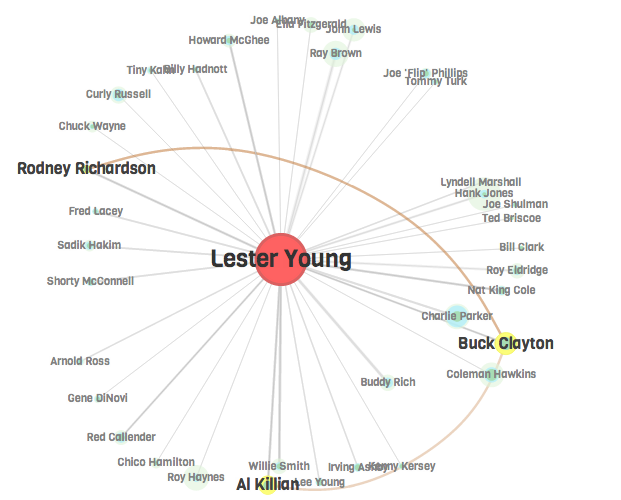
\includegraphics[width=0.8\linewidth]{figures/lester-young}
    \caption{\textbf{Hops reveal ego network connectivity.} Additional ``hops'' edges show past collaborations between periphery nodes that did not include the main musician. Here, Buck Clayton had recorded with Rodney Richardson and Al Killian numerous times prior to working with Lester Young.}
    \label{fig:moj:young}
  \end{figure}


%%%%%%%%%%%%%%%%%%%%%%%%%%%%%%%%%%%%%%%%%%%%%%%%%%%%%%%%%%%%%%%%%%%%%%%%%%%%%%%
\section{Discussion and Conclusions}

  The Map of Jazz approaches the problem of dynamic graph visualization from a new angle: instead of tackling the problem of visualizing large graphs in general and tracking temporal changes on a global scale, the Map focuses on individual nodes and local changes that would have an immediate and personal effect. The Map of Jazz arranges related nodes into an ego-network with a single individual in the center surrounded by close neighbors who are placed according to the strength of their connection with the central node. Users can explore the dynamic properties of the network by dragging the time slider or zooming in on a particular era of interest. The ego-network adjusts the node positions according to the varying strength of their connection to the central node during that time. The appearance of nodes and edges updates as well to reflect the change in their attributes.

  We tailor our visualization to assist the exploration of a novel jazz collaboration network. In social interactions, the frequency and recency of interactions determine the strength of the collaboration between individuals. We propose and implement a collaboration strength function that takes into account both past and future interactions and helps quantify the strength of the relationship between the two musicians at any point in time.

  The concepts developed for the Map of Jazz can be applied to other networks that record multiple interactions between entities and to dynamic networks in general, especially those where the numerical attributes on nodes and edges change over time. One such example is the gene co-expression network where genes control the expression of other genes in the cell. The amount of one gene product may change over the natural cycle of a cell (cell division, growth, death) and affect the behavior of related genes. 
  %
  % XXX: Russell -- in what ways might dynamic biological networks differe from jaz networks? Do the networks have similar properties and does that matter for the algorithms?
  %
  Much like the social networks, biological networks have been shown to be sparse and scale-free with few ``promiscuous'' nodes regulating many other nodes in the graph and thus affecting many of the cell processes. Analyzing the interactions of such high degree nodes over time or varying conditions through a visualization like Map of Jazz can provide insights to the complex relationships between genes and their products within the cell.
  Applications to other collaboration networks such as co-authorship data are straightforward.
  



%%%%%%%%%%%%%%%%%%%%%%%%%%%%%%%%%%%%%%%%%%%%%%%%%%%%%%%%%%%%%%%%%%%%%%%%%%%%%%%
%%
%% Domains -- inferring high-level structure from DNA conformation data
%%
%%%%%%%%%%%%%%%%%%%%%%%%%%%%%%%%%%%%%%%%%%%%%%%%%%%%%%%%%%%%%%%%%%%%%%%%%%%%%%%
% algorithms for managing biological data
\chapter{Identifying topological domains in ensembles of chromosome contacts}
\label{chapter:domains}


Recent high-throughput experiments on chromatin conformation capture (3C) and its variants provide indirect measurement of spatial proximity between genomically disjoint parts of folded nuclear DNA in living cells. These data have significantly advanced our understanding of the geometry of chromatin structure~\cite{Gibcus2013}, of the relationship between chromatin structure and the regulation of gene expression, nuclear organization, cancer translocations~\cite{Cavalli2013}, and copy number alterations in cancer~\cite{Fudenberg2011}. The experimental protocol starts with a cross-linking of chromatin using formaldehyde thus ensuring that parts of chromatin that are spatially close are affixed to each other. The bound chromatin is then isolated, the fragments of DNA protected by the chromatin extracted and ligated. After a series of amplifications, these DNA fragments are mapped to a reference genome and their abundance quantified across the whole population of cells participating in the experiment~\cite{Dekker3c}. In this way, 3C data is an aggregate of multiple observations of chromatin contacts over many cells and is similar to the classification data analyzed in Coral (Chapter~\ref{chapter:coral}). 

A prominent feature of 3C experimental results are genomically contiguous regions of dense 3C interactions --- the so-called \textit{topological domains} --- that affect accessibility of certain regions of DNA and are associated with long-range gene regulation. These megabase-sized topological domains are persistent across cell types and are conserved across species~\cite{Dixon2012}. Topological domains are strongly correlated with a number of chromatin markers and have been included in a number of analyses since their discovery~\cite{Hou2012,Kolbl2012,Lin2012}, additionally, they were found to serve as a skeleton for the placement of many functional elements of the genome~\cite{Bickmore2013a,Tanay2013}. However, visual analysis of the 3C interaction matrices strongly suggests that functionally-relevant domains may exist at multiple length scales, can overlap with other domains, and may be a part of multiple optimal structures. We notice the striking similarity between the problems of finding sets of persistent annotations in Coral (Chapter~\ref{chapter:coral}) and identification of topological domains in chromatin and adapt the core finding algorithm discussed in Section~\ref{sec:dense_sub} to find novel domain structures.

% (from intro) We extend the algorithm for identifying robust subsets of annotations from our ear- lier work to the problem of finding densly packed areas of chromatin (topological domains). 

Our algorithm is fast, requires fewer parameters than existing methods, and is able to capture topological domains at different resolutions. It generates domains that are similar, yet significantly different from domains identified by existing methods. These domains are smaller, capture more of the high-frequency chromatin interactions, and are more enriched for the chromatin markers associated with gene regulation. The ability to obtain domains at different scales allows us to evaluate and quantify the extent of the hierarchical structure of the chromatin for the first time~\cite{ArmatusAMB}.


% We introduce a new and efficient algorithm that is able to capture persistent domains across various resolutions by adjusting a single scale parameter. The identified novel domains are substantially different from domains reported previously and are highly enriched for insulating factor CTCF binding and histone modfications at the boundaries.

The work described in this chapter has been presented at Workshop for Algorithms in Bioinformatics 2013 (WABI)~\cite{Filippova2013} and was extended to extract alternative optimal and near-optimal solutions. Further, this ensemble of solutions was used to quantify the strength of hierarchical organization between domains at different resolutions~\cite{ArmatusAMB}. The algorithms are implemented in software Armatus which could be downloaded from \url{https://github.com/kingsfordgroup/armatus}.

%%%%%%%%%%%%%%%%%%%%%%%%%%%%%%%%%%%%%%%%%%%%%%%%%%%%%%%%%%%%%%%%%%%%%%%%%%%%%%%
\section{Background and related work}

  \subsection{Chromosome conformation data}

  % Chromatin interactions obtained from a variety of recent experimental techniques in chromosome conformation capture (3C)~\cite{DeWit2012} have resulted in significant advances in our understanding of the geometry of chromatin structure~\cite{Gibcus2013}, its relation to the regulation of gene expression, nuclear organization, cancer translocations~\cite{Cavalli2013}, and copy number alterations in cancer~\cite{Fudenberg2011}.  

  % Of these advances, the recent discovery of dense, contiguous regions of chromatin termed \emph{topological domains}~\cite{Dixon2012} has resulted in the incorporation of domains into many subsequent analyses~\cite{Hou2012,Kolbl2012,Lin2012} due to the fact that they are persistent across cell types, conserved across species, and serve as a skeleton for the placement of many functional elements of the genome~\cite{Bickmore2013a,Tanay2013}.


  %%%%%%%%%%%%%%%%%%%%%%%%%%%%%%%%
  % heatmap figure with domains
  %%%%%%%%%%%%%%%%%%%%%%%%%%%%%%%%
  \begin{figure}[t!]
    \begin{center}
      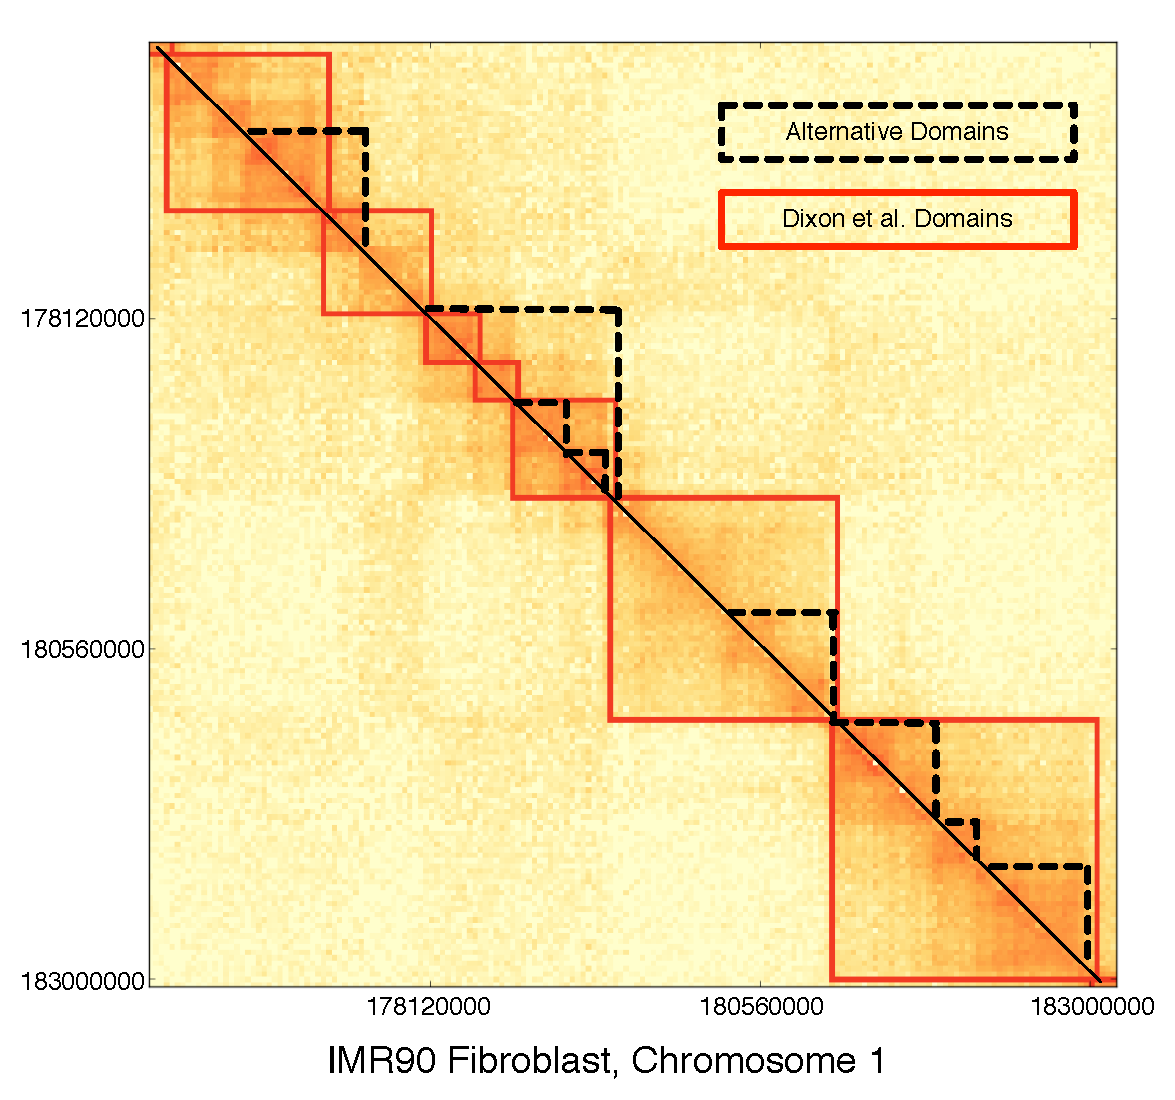
\includegraphics[width=3in]{figures/HeatMapFig}
    \end{center}
    \caption{\textbf{Interaction matrix for a portion of human chromosome 1} from a recent Hi-C experiment by Dixon et al.~\cite{Dixon2012}. Each axis represents a location on the chromosome (40kbp bins).  Densely interacting domains identified by the method of Dixon et al. (red boxes).  Alternative domains are shown as dotted black lines on the upper triangular portion of the matrix.  Visual inspection of the lower triangular portion suggests domains could be completely nested within another and highly overlapping when compared to Dixon et al.'s domains. This motivates the problem of identifying alternative domains across length scales.}
    \label{armatus:heatmap}
  \end{figure}


  3C experiments result in matrices of counts that represent the frequency of cross-linking between restriction fragments of DNA that are spatially near one another (see Figure~\ref{armatus:heatmap} for an example matrix). $X$ and $Y$ axes represent a genomic coordinate along a single chromosome (although a later HI-C protocol~\cite{HiCProtocol} is able capture interactions across chromosomes as well), and a single point in the matrix represents a number of times two corresponding DNA fragments were found to interact. The original identification of domains in Dixon et al.~\cite{Dixon2012} employed a Hidden Markov Model (HMM) on these interaction matrices to identify regions initiated by significant downstream chromatin interactions and terminated by a sequence of significant upstream interactions.  A defining characteristic of the domains resulting from their analysis is that higher frequency 3C interactions tend to occur within domains as opposed to across domains. This aspect of domains is also reflected in the block-diagonal structure of 3C interaction matrices as shown in Figure~\ref{armatus:heatmap}. In this sense, domains can be interpreted as contiguous genomic regions that self-interact frequently and are more spatially compact than their surrounding regions.

  %%%%%%%%%%%%%%%%%%%%%%%%%%%%%%%%
  \subsection{Topological domains and their significance}

  However, the single collection of megabase-sized domains may not be the only topologically and functionally relevant collection of domains. On closer inspection of the block-diagonal matrix structure in Figure~\ref{armatus:heatmap}, it becomes clear that there are alternative contiguous regions of the chromosome that self-interact frequently and are likely more spatially compact than their surrounding regions (dotted lines).  Some of these regions appear to be completely nested within others, suggesting a hierarchy of compact regions along the chromosome, while others appear to overlap each other. These observations suggest that functionally-relevant chromosomal domains may exist at multiple scales.

  We introduce a new algorithm to efficiently identify topological domains in 3C interaction matrices for a given domain-length scaling factor $\gamma$. Our results suggest that there exist a handful of characteristic resolutions across which domains are similar. Based on this finding, we identify a consensus set of domains that persist across various resolutions. We find that domains discovered by our algorithm are dense and cover interactions of higher frequency than inter-domain interactions. Additionally, we show that inter-domain regions within the consensus domain set are highly enriched with insulator factor CTCF and histone modification marks. We argue that our straightforward approach retains the essence of the more complex multi-parameter HMM introduced in~\cite{Dixon2012} while allowing for the flexibility to identify biologically relevant domains at various scales.


%%%%%%%%%%%%%%%%%%%%%%%%%%%%%%%%%%%%%%%%%%%%%
%
% Problem definition
%
%%%%%%%%%%%%%%%%%%%%%%%%%%%%%%%%%%%%%%%%%%%%%
\section{Problem formulation}


  \theoremstyle{definition}
  \newtheorem{prob}{Problem}

  Given the resolution of the 3C experiment (say, 40kb), the chromosome is broken into $n$ evenly sized fragments. 3C contact maps record interactions between different sections of the chromosome in the form of a weighted adjacency matrix $\mathbf{A}$ where two fragments $i$ and $j$ interact with frequency $\mathbf{A}_{ij}$.

  \begin{prob}[Resolution-specific domains] \label{domainprob} Given a $n \times n$ weighted adjacency matrix $\mathbf{A}$ and a resolution parameter $\gamma \geq 0$, we wish to identify a set of domains $D_{\gamma}$ where each domain is represented as an interval $d_i=[a_i, b_i]$, $1 \leq a_i < b_i \leq n$ such that no two $d_i$ and $d_j$ overlap for any $i \ne j$. Additionally, each domain should have a larger interaction frequency within domain than to its surrounding regions.

  Here, the parameter $\gamma$ is inversely related to the average domain size in $D_{\gamma}$: lower $\gamma$ results in sets of larger domains and higher $\gamma$ corresponds to sets of smaller domains. We define $\gamma$ and discuss it in more detail later in the text.

  Specifically, we seek to identify a set of non-overlapping domains $D_{\gamma}$ that optimize the following objective:
  %
  \begin{align}
    \label{obj}
    \max \sum_{[a_i,b_i] \in D_{\gamma}} q(a_i,b_i,\gamma),
  \end{align}
  %
  where $q$ is a function that quantifies the quality of a domain $[a_i, b_i]$ at resolution $\gamma$. Since domains are required to contain consecutive fragments of the chromosome, this problem differs from the problem of clustering the graph of 3C interactions induced by $\mathbf{A}$, since such a clustering may place non-contiguous fragments of the chromosome into a single cluster. In fact, this additional requirement allows for an efficient optimal algorithm.
  \end{prob}

  \begin{prob}[Consensus domains across resolutions]
  \label{consensusprob}  Given $\mathbf{A}$ and a
  set of resolutions $\Gamma = \{\gamma_1, \gamma_2, \ldots \}$, identify a set of non-overlapping domains $D_c$ that are most persistent across resolutions in $\Gamma$:
  \begin{align}
  \label{consobj}
  \max \sum_{[a_i,b_i] \in D_c} p(a_i,b_i,\Gamma),
  \end{align}
  where $p(a_i,b_i,\Gamma)$ is the persistence of domain $[a_i, b_i]$ corresponding to how often it appears across resolutions.
  \end{prob}

\section{Algorithms}



  %%%%%%%%%%%%%%%%%%%%%%%%%%%%%%%%%%%%%%%%%%%%%
  %
  %%%%%%%%%%%%%%%%%%%%%%%%%%%%%%%%%%%%%%%%%%%%%
  \subsection{Domain identification at a particular resolution}
  \label{singleres}
  Since each row and corresponding column in a 3C interaction matrix encodes a genomic position on the chromosome, we can write the solution to objective~(\ref{obj}) as a dynamic program:
  %
  \begin{align}
    \label{pbd}
    \textsf{OPT}_1(l) = \max_{k<l}\{\textsf{OPT}_1(k-1) + \max\{q(k,l,\gamma),0\}\},
  \end{align}
  %
  where $\textsf{OPT}_1(l)$ is the optimal solution for objective~(\ref{obj}) for the sub-matrix defined by the first $l$ positions on the chromosome ($\textsf{OPT}_1(0) = 0$). The choice of $k$ encodes the size of the domain immediately preceding location $l$. We define negative-scoring domains as non-domains and, as such, only domains with $q > 0$ in the max term in~(\ref{pbd}) are retained.

  Our quality function $q$ is:
  %
  \begin{align}
    \label{quality} q(k,l,\gamma) &= s(k,l,\gamma)-\mu_s(l-k),\mbox{ where}\\
    \label{sumtri} s(k,l,\gamma) &= \frac{\sum_{g=k}^l \sum_{h=g+1}^l A_{gh}}{(l-k)^\gamma}
  \end{align}
  %
  is a \emph{scaled density} of the subgraph induced by the interactions $A_{gh}$ between genomic loci $k$ and $l$. Equation~(\ref{quality}) is the zero-centered sum of~(\ref{sumtri}), which is the upper-triangular portion of the submatrix defined by the domain in the interval $[k,l]$ divided by the scaled length $(l-k)^{\gamma}$ of the domain. When $\gamma=1$,  the scaled density is the weighted subgraph density~\cite{goldberg1984finding} for the subgraph induced by the fragments between $k$ and $l$. When $\gamma=2$, the scaled density is half the internal density of a graph cluster~\cite{Schaeffer2007}. For larger values of $\gamma$, the length of a domain in the denominator is amplified, hence, smaller domains would produce larger objective values than bigger domains with similar interaction frequencies. $\mu_s(l-k)$ is the mean value of~(\ref{sumtri}) over all sub-matrices of length $l-k$ along the diagonal of $\mathbf{A}$, and can it be pre-computed for a given $\mathbf{A}$. We disallow  domains where there are fewer than 100 sub-matrices available to compute the mean. By doing this, we are only excluding domains of size larger than $n-100$ fragments, which in practice means that we are disallowing domains that are  hundreds of megabases long.  Values for the numerator in (\ref{sumtri}) are also pre-computed using an efficient algorithm~\cite{Filippova2012}, resulting in an overall run-time of $O(n^2)$ to compute $\textsf{OPT}_1(n)$.

  %%%%%%%%%%%%%%%%%%%%%%%%%%%%%%%%%%%%%%%%%%%%%
  % Consensus set - persistence
  %%%%%%%%%%%%%%%%%%%%%%%%%%%%%%%%%%%%%%%%%%%%%
  \subsection{Obtaining a consensus set of persistent domains across resolutions}
  \label{consensusalg}
  For objective (\ref{consobj}), we use the procedure in section~\ref{singleres} to construct a set $\mathcal{D} = \bigcup_{\gamma \in \Gamma} D_{\gamma}$.  $\mathcal{D}$ is a set of overlapping intervals or domains, each with a quality score defined by its persistence $p$ across resolutions. To extract a set of highly persistent, non-overlapping domains from $\mathcal{D}$, we reduce  problem~\ref{consensusprob} to the weighted interval scheduling problem~\cite{Kleinberg2005}, where competing requests to reserve a resource in time are resolved by finding the highest-priority set of non-conflicting requests. To find a consensus set of domains, we map a request associated with an interval of time to a domain and its corresponding interval on the chromosome. The priority of a request maps to a domain's persistence $p$ across length scales.

  The algorithm to solve problem~\ref{consensusprob} is then:
  \begin{align}
  \label{wis}
  \textsf{OPT}_2(j) = \max\{\textsf{OPT}_2(j-1), \textsf{OPT}_2(c(j)) + p(a_j,b_j,\Gamma) \}
  \end{align}
  where $\textsf{OPT}_2(j)$ is the optimal non-overlapping set of domains for the $j$th domain in a list of domains sorted by their endpoints ($\textsf{OPT}_2(0) = 0$), and $c(j)$ is the closest domain before $j$ that does not overlap with $j$.  The first and second terms in~(\ref{wis}) correspond to either choosing or not choosing domain $j$ respectively.
  We pre-compute a domain's persistence $p$ as:
  \begin{align}
  \label{persist}
  p(a_i,b_i,\Gamma) = \sum_{\gamma \in \Gamma} \delta_i \text{ where }
  \delta_i = \begin{cases}
  1 & \text{if } [a_i,b_i] \in D_{\gamma} \\ 0 & \text{otherwise.}
  \end{cases}
  \end{align}
  Equation~(\ref{persist}) is therefore a count of how often domain $i$ appears across all resolutions in $\Gamma$ for domain sets identified by the method in section~\ref{singleres}. It may be desirable to treat multiple highly overlapping, non-equivalent domains as a single domain, however, we conservatively identify exact repetitions of a domain across resolutions since this setting serves as a lower bound on the persistence of the domain. If $m=|\mathcal{D}|$, then pre-computing persistence takes $O(m|\Gamma|)$ time, and $c(j)$ is precomputed after sorting the intervals by their endpoints. The limiting factor when computing $\textsf{OPT}_2(m)$ is time to compute $c(j)$, which is $m\log m$. Thus, the overall algorithm runs in $O(m\log m + (n^2+m)|\Gamma|)$ time taking into account an additional $O(n^2|\Gamma|)$ for computing $\mathcal{D}$.


%%%%%%%%%%%%%%%%%%%%%%%%%%%%%%%%%%%%%%%%%%%%%
%
% Results: intrinsic and extrinsic validation of domains, comparison
% to Bing Ren's domains
%
%%%%%%%%%%%%%%%%%%%%%%%%%%%%%%%%%%%%%%%%%%%%%
\section{Results}

  We used chromatin conformation capture data from Dixon et al.~\cite{Dixon2012} for human fibroblast and mouse embryonic cells. The 3C contact matrices were already aggregated at fragment size 40kb and were corrected for experimental bias according to~\cite{Yaffe2011}. We compared our multiscale domains and consensus sets against the domains generated by Dixon et al. for the corresponding cell type and species.
  For human fibroblast cells, we used CTCF binding sites from~\cite{Kim2007}.
  For mouse embryonic cell CTCF binding sites and chromatin modification marks, we used data by Shen et al.~\cite{Shen2012}.

  % List of parameters required by Dixon et al.
  % \begin{itemize}
  % \item 2MB upstream/downstream boundary
  % \item 1-20 mixtures of gaussians
  % \item Median posterior probabilities $\geq 0.99$, at least 80kbp
  % \end{itemize}


  %%%%%%%%%%%%%%%%%%%%%%%%%%%%%%%%%%%%%%%%%%%%%
  % Dense domains
  %%%%%%%%%%%%%%%%%%%%%%%%%%%%%%%%%%%%%%%%%%%%%
  \subsection{Ability to identify densely interacting domains across scales}

  
  %%%%%%%%%%%%%%%%%%%%%%%%%%%%%%%%%%%%
  % inter-intra dist plot; disributions of sizes
  %%%%%%%%%%%%%%%%%%%%%%%%%%%%%%%%%%%%
  % \begin{figure}[t]
  %   \begin{center}
  %   \subfigure[Domain size vs. frequency]{
  %     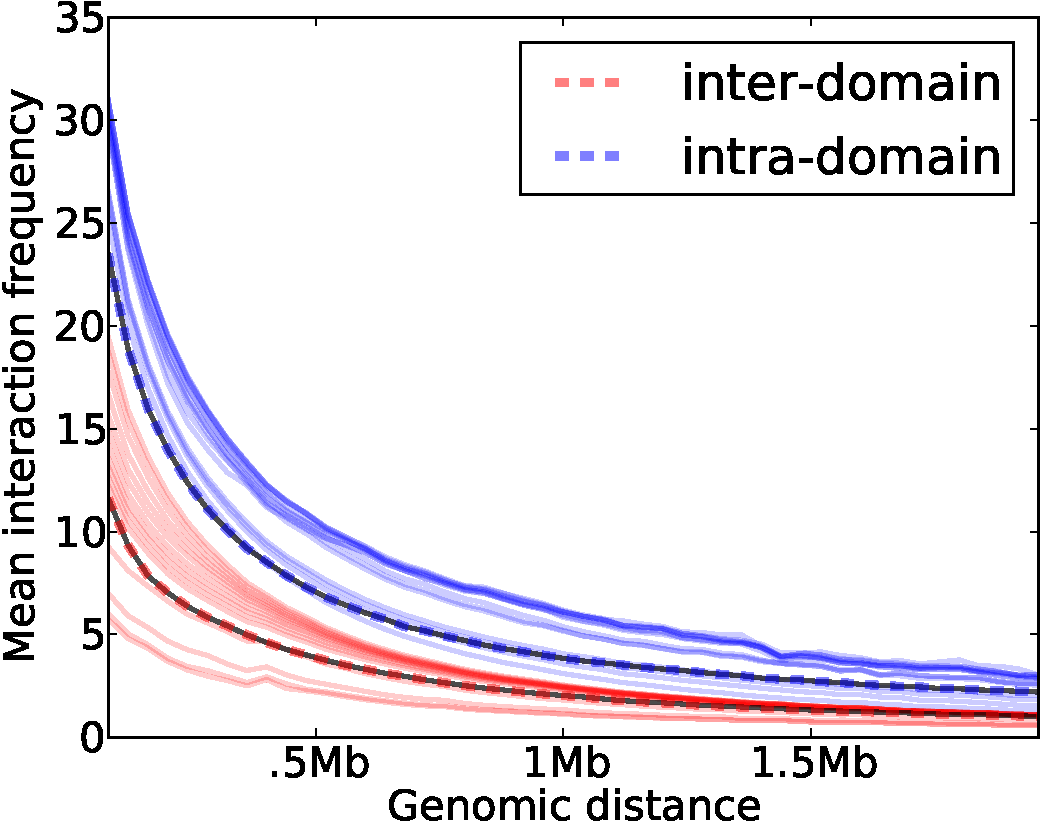
\includegraphics[width=0.45\linewidth]{figures/imr90-inter-intra-all-chromos}
  %     \label{subfig:size-freq}
  %   }
  %   \subfigure[Mean frequency distr.]{
  %     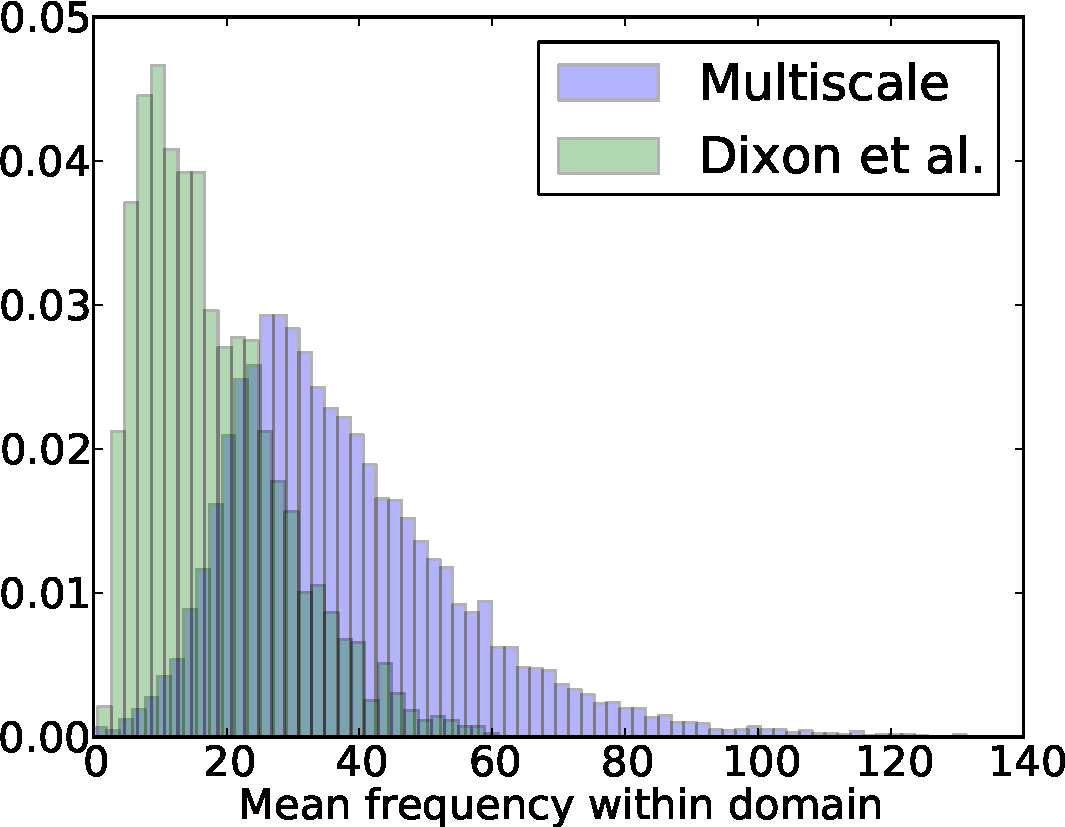
\includegraphics[width=0.45\linewidth]{figures/mean-freq-distr}
  %     \label{subfig:freq-distr}
  %   }
  %   \caption{~\subref{subfig:size-freq}  \subref{subfig:freq-distr}~Multiscale domains identified in human fibroblast cells by our dynamic program tend to have higher mean frequency than those of Dixon et al.
  %   (distributions are plotted after outliers $> \mu+4\sigma$ were removed).}

  %   \label{fig:mi_jacc}
  %   \end{center}
  % \end{figure}

  %%%%%%%%%%%%%%%%%%%%%%%%%%%%%%%%%%%%
  % inter-intra dist plot
  %%%%%%%%%%%%%%%%%%%%%%%%%%%%%%%%%%%%
  \begin{figure}[ht!]
      \centering
    % \subfigure[Domain size vs. frequency]{
      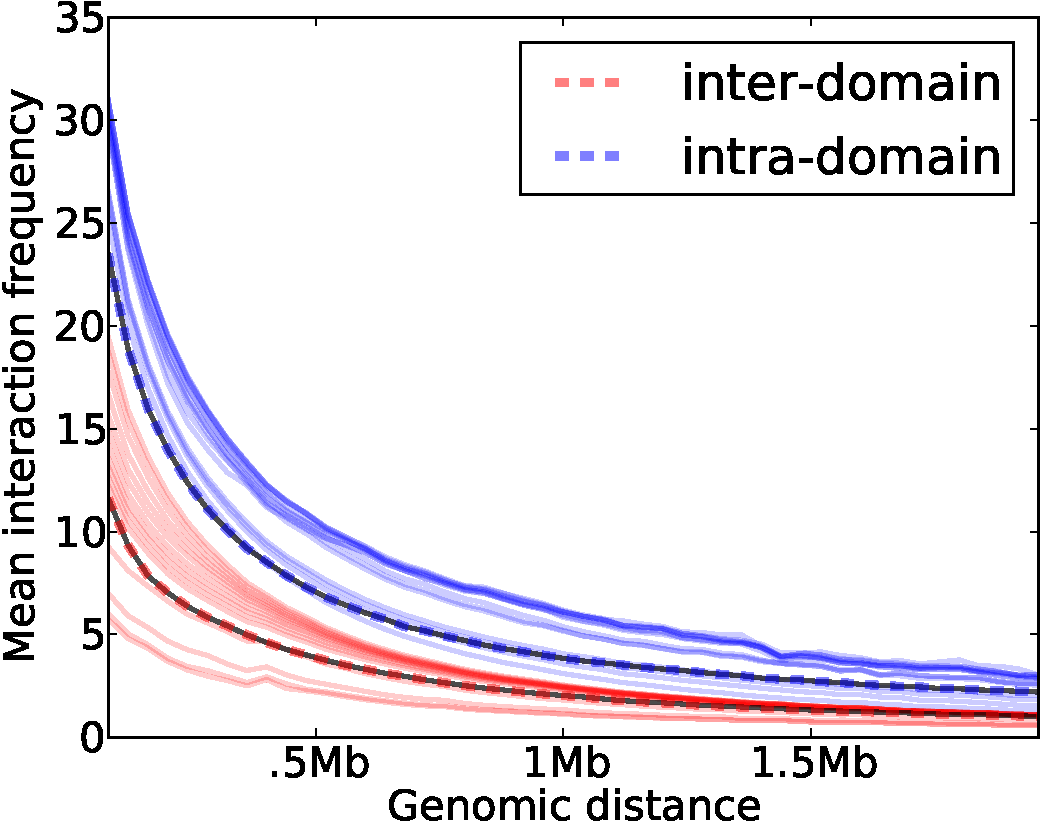
\includegraphics[width=0.6\linewidth]{figures/imr90-inter-intra-all-chromos}
      \caption{\textbf{Domain size vs. frequency.} Our algorithm discovers domains with mean frequency value for inter- and intra-domain interactions (solid lines) at or better than that of Dixon et al.\@ domains (dotted lines). Each solid line represents domains at different resolution $\gamma$ in human fibroblast cells.}
      \label{fig:armatus:size-freq}
    % }
  \end{figure}


  Multiresolution domains successfully capture high frequency interactions and leave interactions of lower mean frequency outside of the domains. We compute the mean interaction frequency for all intra- and inter-domain interactions at various genomic lengths and plot the distribution of means for multiple resolutions (Figure~\ref{fig:armatus:size-freq}). The mean intra-domain interaction frequency (blue) is consistently and up to two times higher than the mean frequency for cross-domain interactions (red). Compared to the domains reported by Dixon et al., our domains tend to aggregate interactions of higher mean frequency, especially at larger $\gamma$. The distribution of mean intra-domain frequencies for Dixon et al.\@ is skewed more to the left than that of the multiscale domains (Figure~\ref{fig:armatus:freq-distr}). This difference can be partially explained by the fact that multiscale domains on average are smaller in size ($\mu=0.2$Mb, $\sigma=1.2$Mb) than domains reported by Dixon et al.\@ ($\mu=1.2$Mb, $\sigma=0.9$Mb).



  %%%%%%%%%%%%%%%%%%%%%%%%%%%%%%%%%%%%
  % disributions of domain sizes
  %%%%%%%%%%%%%%%%%%%%%%%%%%%%%%%%%%%%
  \begin{figure}[ht]
    \centering
    % \subfigure[Domain size vs. frequency]{
      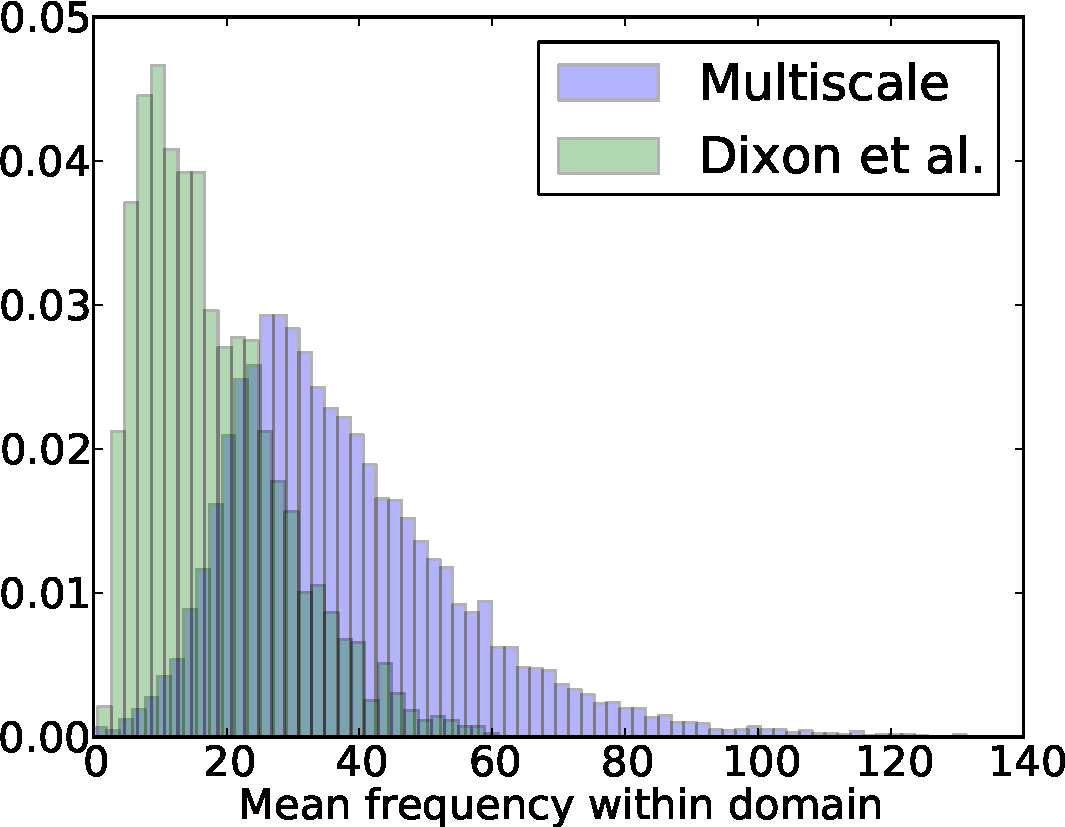
\includegraphics[width=0.6\linewidth]{figures/mean-freq-distr}
      \caption{\textbf{Mean frequency of interactions captured by domains.} Multiscale domains identified in human fibroblast cells by our dynamic program tend to have higher mean frequency than those of Dixon et al. (distributions were plotted after outliers $> \mu+4\sigma$ were removed).}
      \label{fig:armatus:freq-distr}
  \end{figure}



  %%%%%%%%%%%%%%%%%%%%%%%%%%%%%%%%%%%%%%%%%%%%%
  %
  %%%%%%%%%%%%%%%%%%%%%%%%%%%%%%%%%%%%%%%%%%%%%
  \subsection{Domain persistence across scales}

  Domain sets across resolutions share significant similarities, even as the distribution of domains and their sizes begin to change (Figure~\ref{fig:dom_size}). The patterns of similarity are particularly obvious if we plot the domains at various resolutions (Figure~\ref{fig:armatus:domains_line_plot}): many domains identified by our algorithm persist at several resolutions and are aggregated into larger domains at smaller $\gamma$, suggesting a hierarchical domain structure. The stability of these domains across resolutions indicates that the underlying chromosomal structure is dense within these domains and that these domains interact with the rest of the chromosome at a much lower frequency.

  %%%%%%%%%%%%%%%%%%%%%%%%%%%%%%%%%%%%%%%%%%%%
  % Domain sizes over all resolutions, jaccard/overlap/vi between us and b.r.
  % over all resolutions
  %%%%%%%%%%%%%%%%%%%%%%%%%%%%%%%%%%%%%%%%%%%%
  \begin{figure}[t]
    \centering
    \subfigure[domain size \& count vs. $\gamma$]{
        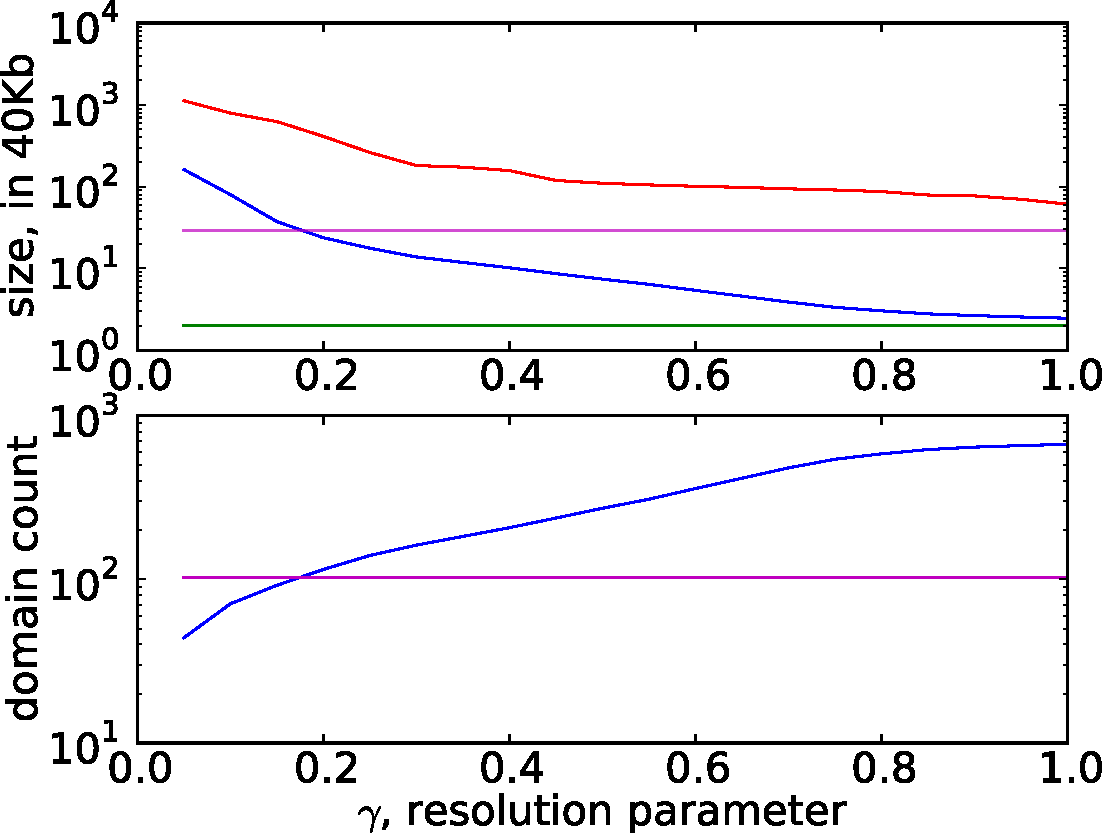
\includegraphics[width=0.46\linewidth]{figures/domain_sizes_all_IMR90.pdf}
        \label{subfig:sizeCount}
    }
    \subfigure[similarity to Dixon et al. domains]{
      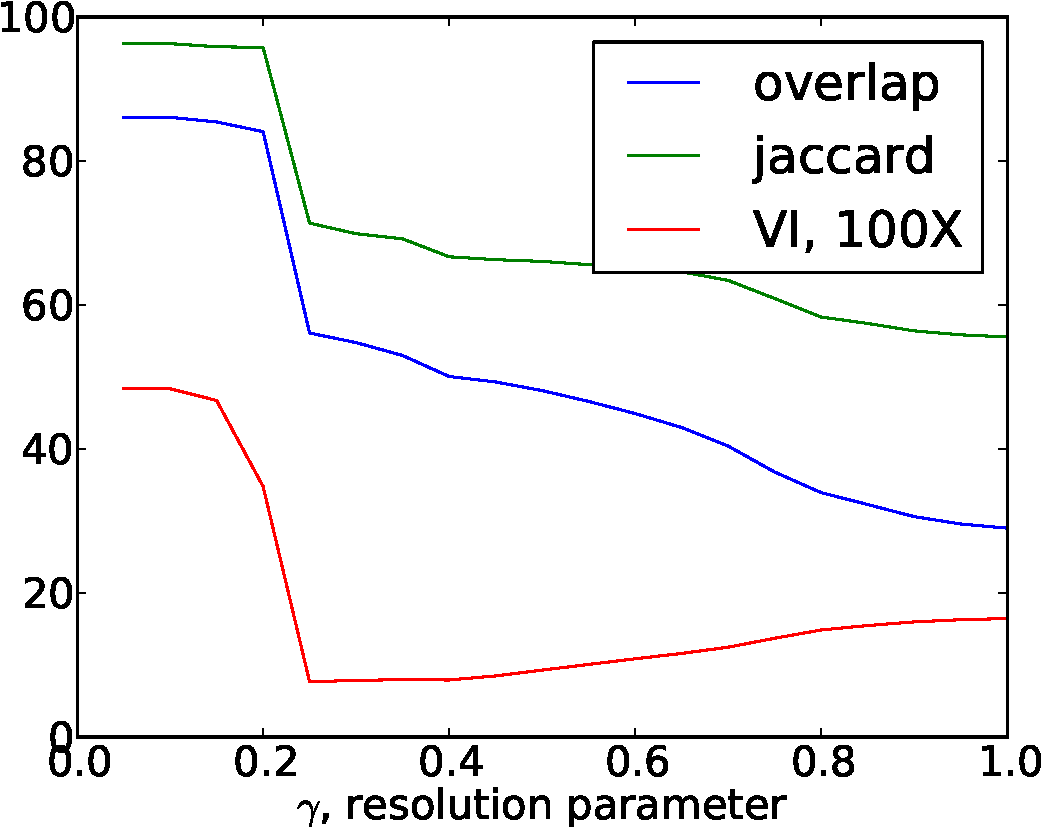
\includegraphics[width=0.43\linewidth]{figures/overlap_br_ours_chr1.pdf}
      \label{subfig:dixonSim}
    }
    \caption{~\subref{subfig:sizeCount} The domain sizes increase and the domain count decreases as the resolution parameter drops. Above: plotted are maximum (red), average (blue), and minimum (green) domain size averaged over all chromosomes for the domains on human fibroblasts. The magenta line shows the average domain size for domains reported by Dixon et al. Below: the number of domains increases for higher values of resolution parameter. The magenta line displays domain count for Dixon et al.~\subref{subfig:dixonSim} According to the Jaccard metric, the similarity between multiresolution domains and domains reported by Dixon et al. increases as the resolution parameter goes to zero.}%, however, the variation of information suggests that the two sets of domains are most similar around $\gamma=0.25$.}
    \label{fig:dom_size}
  \end{figure}




  %%%%%%%%%%%%%%%%%%%%%%%%%%%%%%%%%%%%%%%%%%%%
  % Domains at different resolutions as a line plot
  %%%%%%%%%%%%%%%%%%%%%%%%%%%%%%%%%%%%%%%%%%%%
  \begin{figure}[ht]
    \centering
    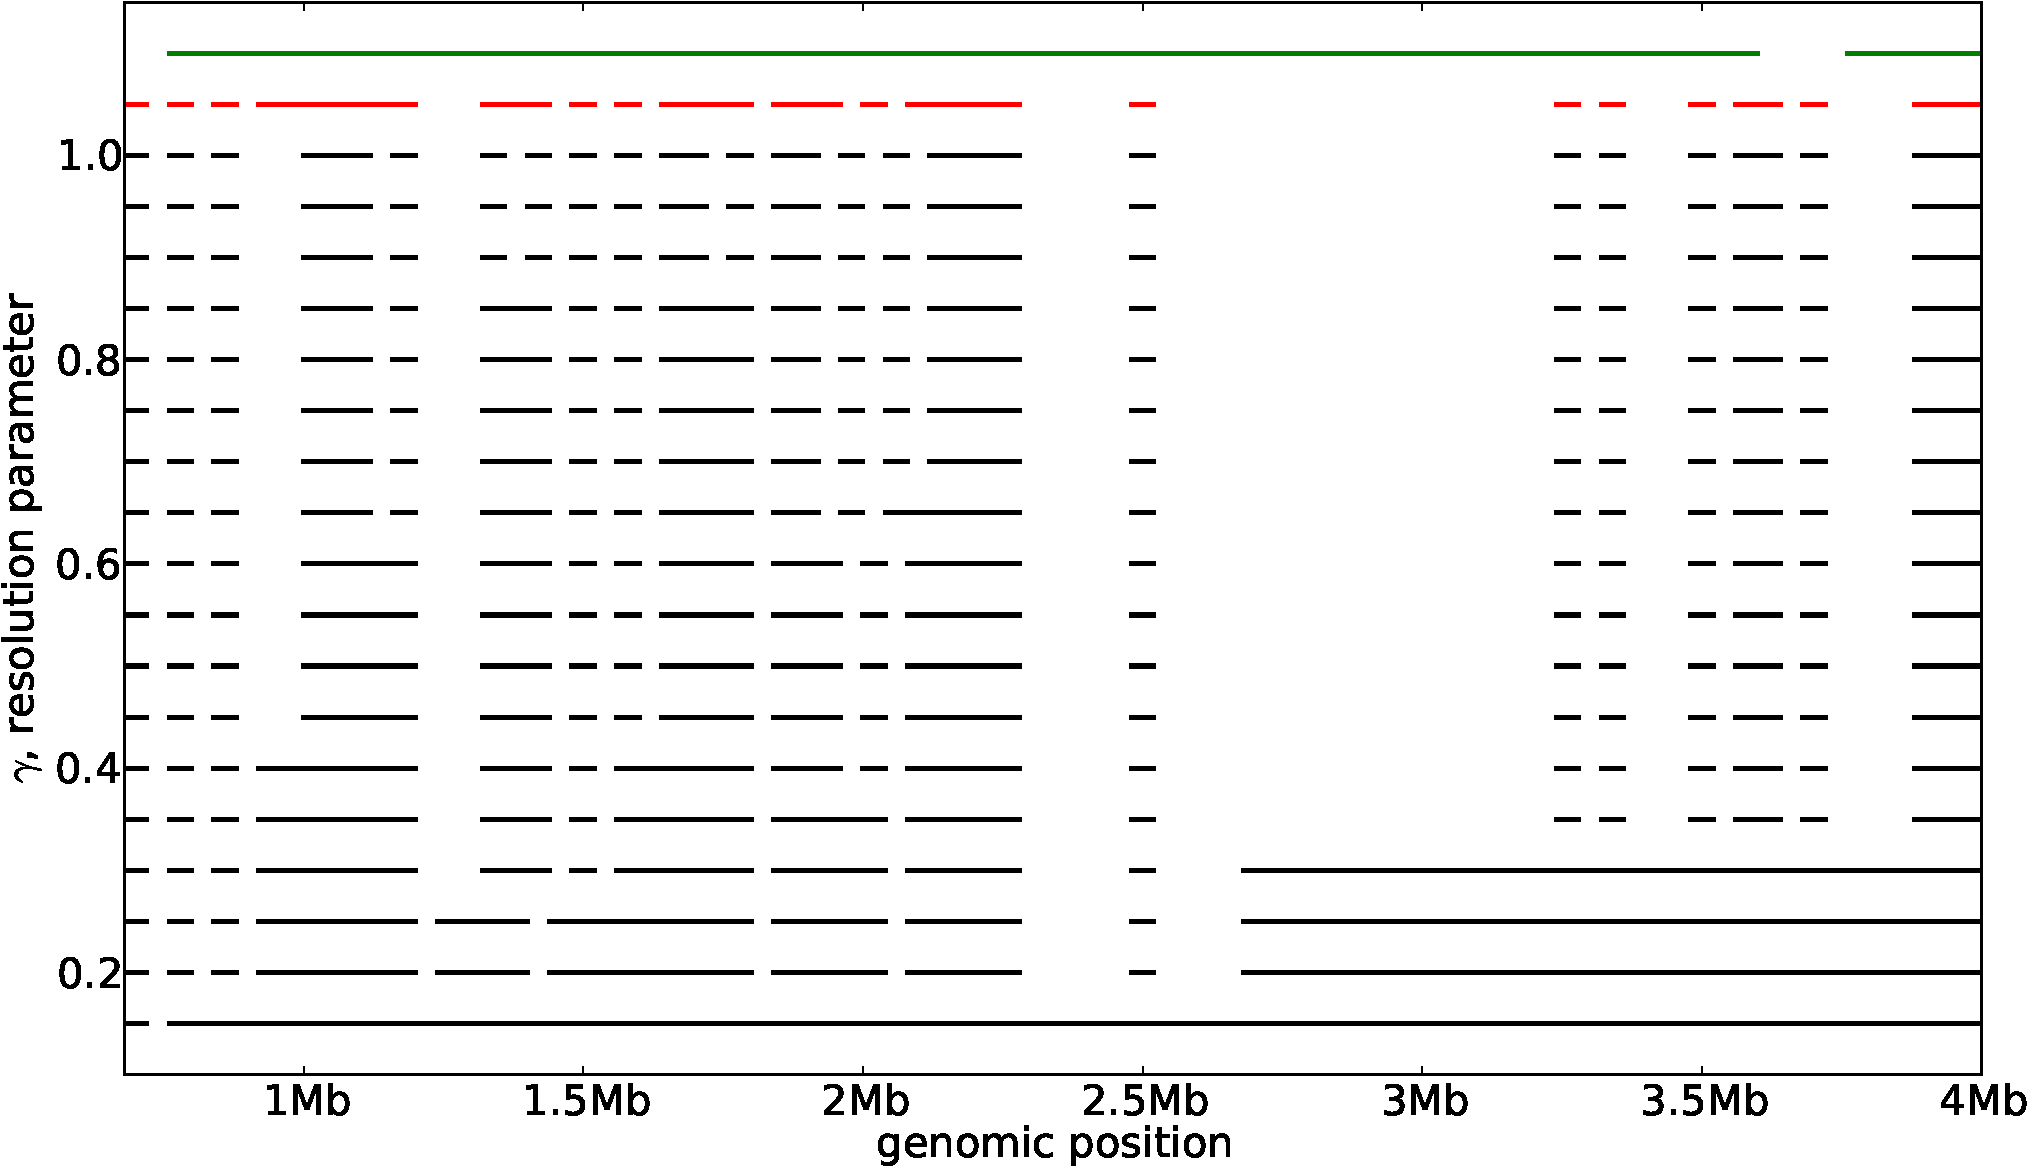
\includegraphics[width=0.9\linewidth]{figures/domains_long_chr1}
    \caption{\textbf{Domains compared across resolutions.} Domains identified by our algorithm (black) are smaller at higher resolutions and merge to form larger domains at $\gamma$ close to 0. Visual inspection shows qualitative differences between consensus Armatus domains (red) and domains reported by Dixon et al. (green). Data shown for the first 4Mb of chromosome 1.}
    \label{fig:armatus:domains_line_plot}
  \end{figure}


  A pairwise comparison of domain configurations displays regions of stability across multiple resolutions (Figure~\ref{fig:armatus:domains_vi}). We use the variation of information (VI)~\cite{Meila2003}, a metric for comparing two sets of clusters, to compute the distance between two sets of domains. To capture the similarities between two domain sets $D$ and $D'$ and the inter-domain regions induced by the domains, we construct new derivate sets $C$ and $C'$ where $C$ contains all domains $d \in D$ as well as all inter-domain regions ($C'$ is computed similarly). To compute entropy of a set of domains $H(C) = \sum_{c_i  \in C} p_i \log p_i$, we define the probability of seeing each interval in $C$ as:
  %
  \[
    p_i = (b_i - a_i) / L,
  \]
  %
  where $L$ is the number of nucleotides from the start of the leftmost domain to the end of the rightmost domain in the set $D \cup D'$. When computing the mutual information between two sets of intervals $C$ and $C'$:
  %
  \[
    I(C, C') = \sum_{c_i \in C} \sum_{c'_j \in C'} p_{ij} \log[ p_{ij} / (p_i p_j) ],
  \]
  %
  we define the joint probability $p_{ij}$ to be:
  %
  \[
    p_{ij} = | [a_i, b_i] \cap [a_j, b_j] | / L.
  \]
  %
  We then compute variation of information on these two new sets: $VI(C, C') =  H(C) + H(C') - 2I(C, C')$ where $H(\cdot)$ is entropy and $I(\cdot, \cdot)$ is mutual information. Chromosome 1, for example, has three visually pronounced groups of resolutions within which domain sets tend to be more similar than across ($\gamma = $[0.00-0.20], [0.25-0.70], and [0.75-1.00] --- see Figure~\ref{fig:armatus:domains_vi}).


  %%%%%%%%%%%%%%%%%%%%%%%%%%%%%%%%%%%%%%%%%%%%
  % Domains at different resolutions as a line plot
  %%%%%%%%%%%%%%%%%%%%%%%%%%%%%%%%%%%%%%%%%%%%
  % \begin{figure}[t]
  %   \begin{center}
  %   \subfigure[domains across resolutions]{
  %     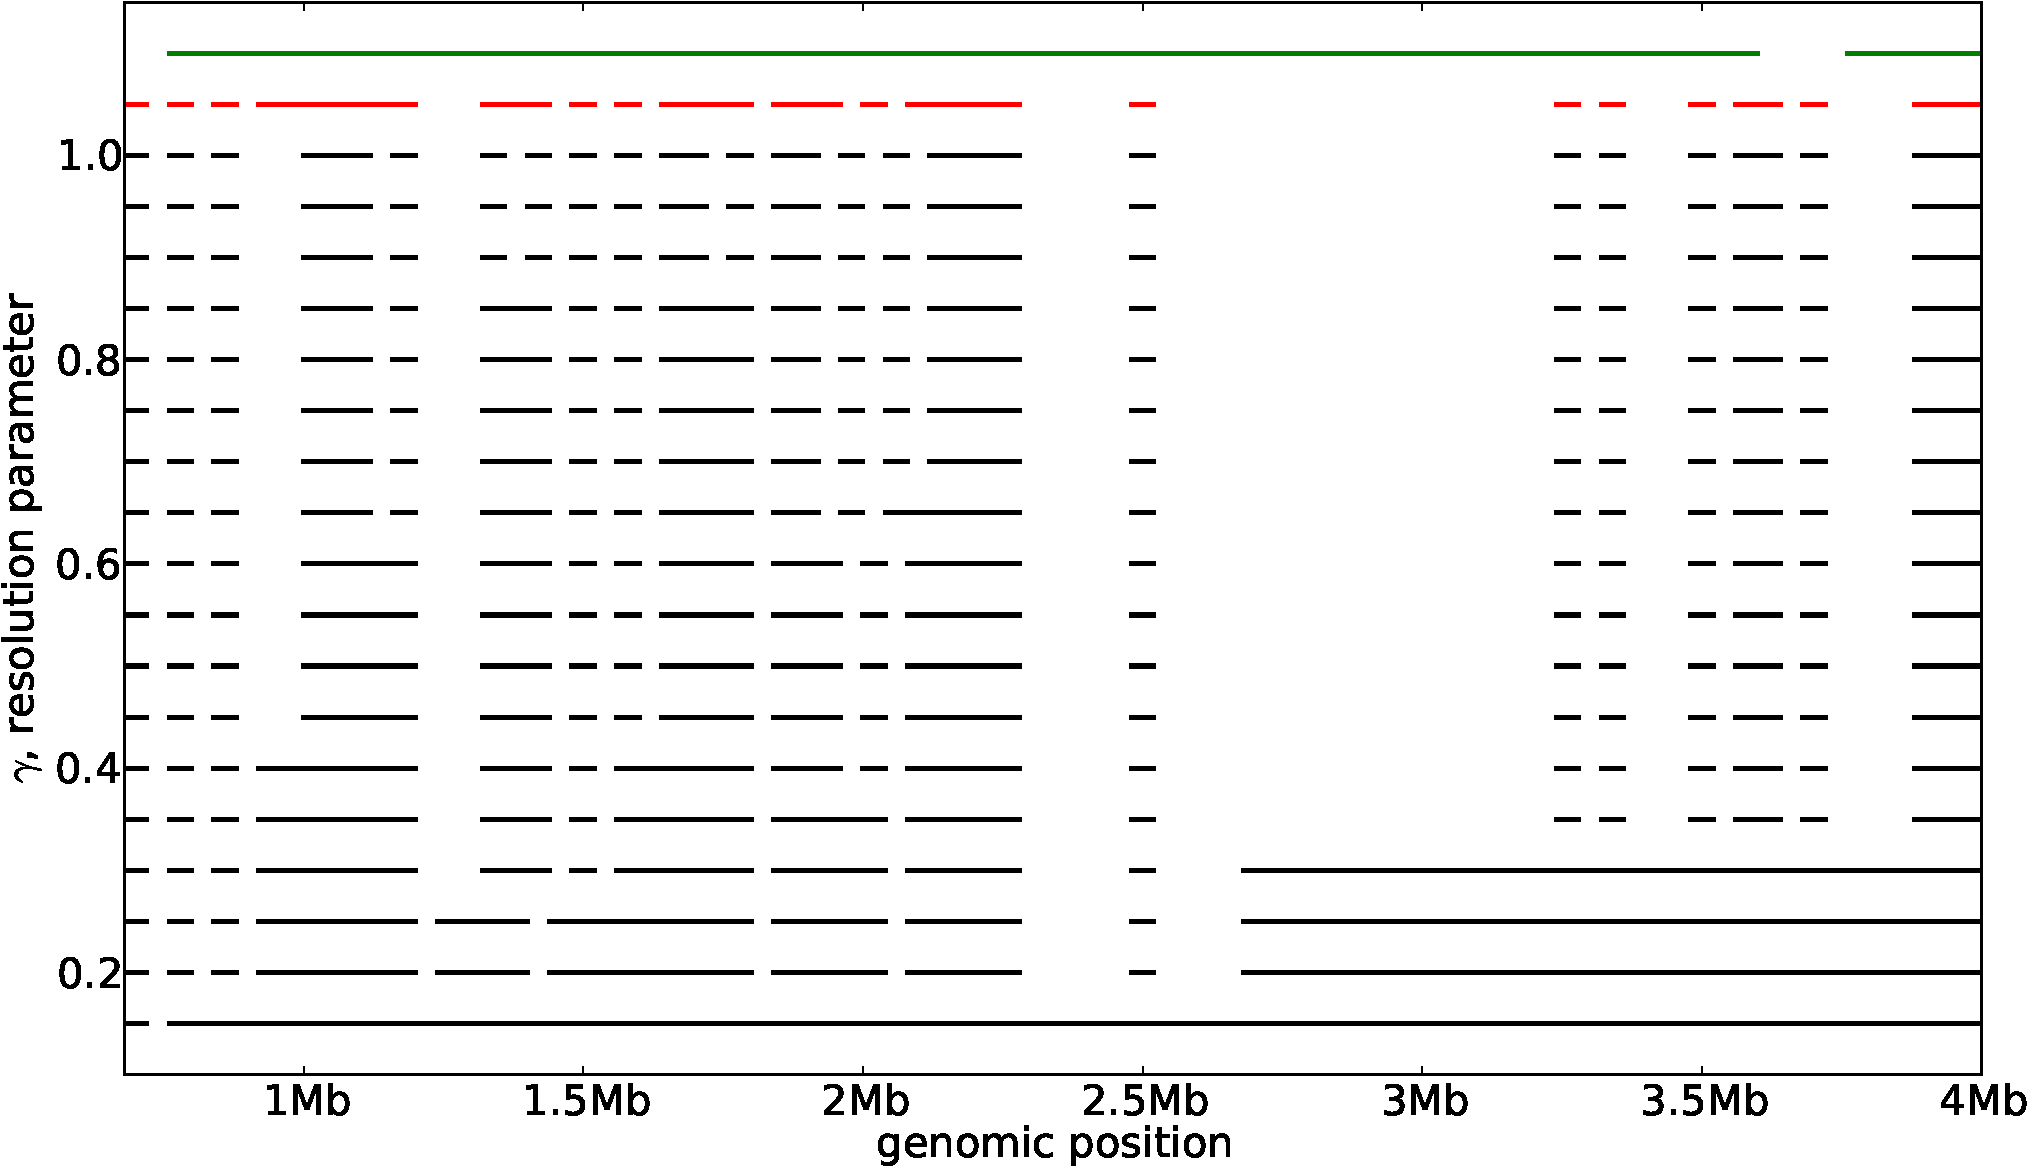
\includegraphics[width=0.55\linewidth]{figures/domains_long_chr1}
  %     \label{fig:armatus:domains_line_plot}
  %   }
  %   \subfigure[VI across resolutions]{
  %     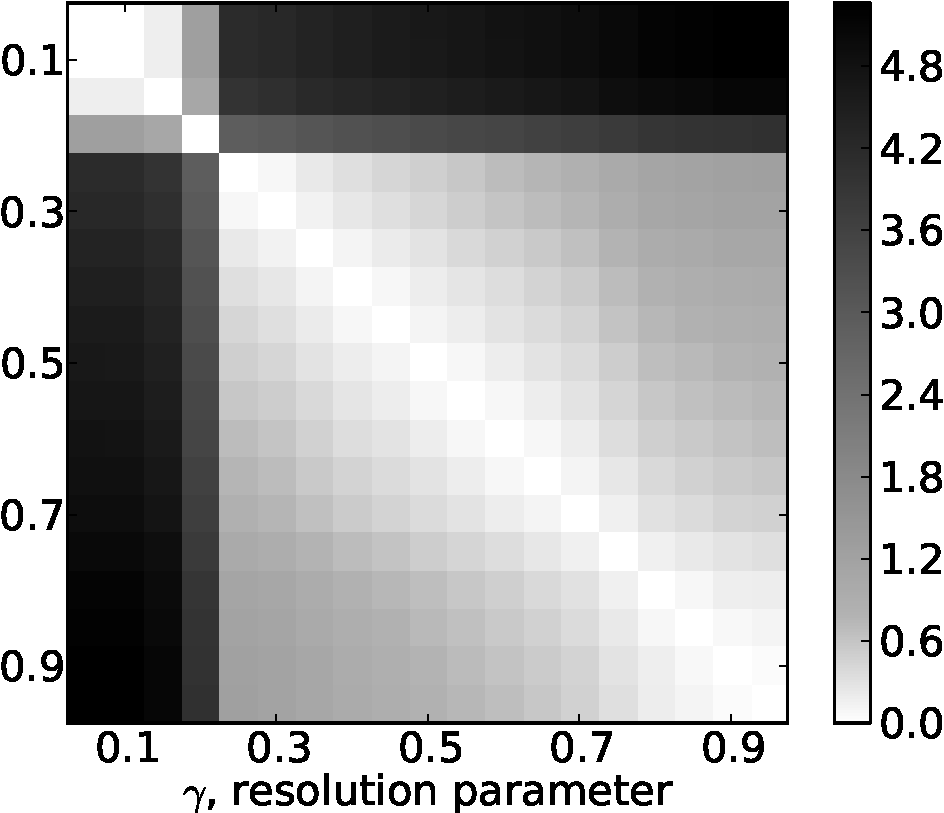
\includegraphics[width=0.366\linewidth]{figures/vi_chr1}
  %     \label{fig:armatus:domains_vi}
  %   }
  %   \end{center}
  %   \caption{~\subref{fig:armatus:domains_line_plot} Domains identified by our algorithm (black) are smaller at higher resolutions and merge to form larger domains at $\gamma$ close to 0. Visual inspection shows qualitative differences between consensus domains (red) and domains reported by Dixon et al. (green). Data shown for the first 4Mb of chromosome 1.~\subref{fig:armatus:domains_vi} Variation of information for domains identified by our algorithm across different resolutions for chromosome 1 in human fibroblast cells.}
  %   \label{fig:domains_line}
  % \end{figure}

  


  %%%%%%%%%%%%%%%%%%%%%%%%%%%%%%%%%%%%%%%%%%%%
  % VI for domains at different resolutions
  %%%%%%%%%%%%%%%%%%%%%%%%%%%%%%%%%%%%%%%%%%%%
  \begin{figure}[ht]
    \centering
    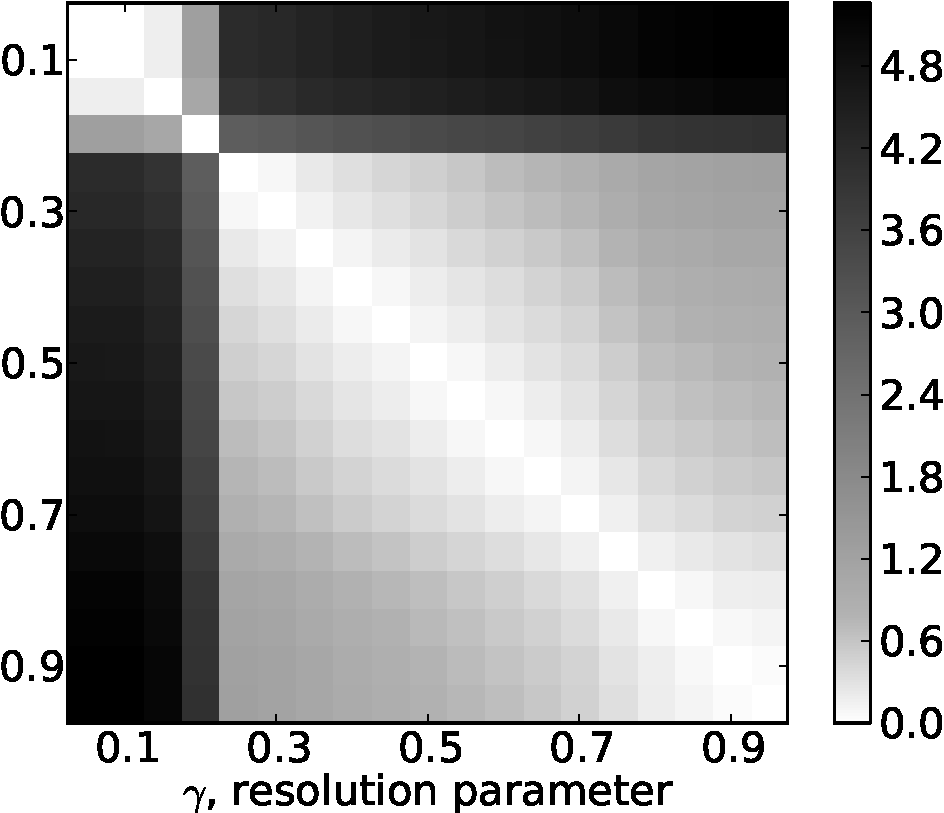
\includegraphics[width=0.5\linewidth]{figures/vi_chr1}
    \caption{\textbf{Variation of information for Armatus domains across resolutions.}}
    \label{fig:armatus:domains_vi}
  \end{figure}


  \subsection{Comparison with the previously identified set of domains in Dixon et al.}

  \begin{figure}[ht]
    \begin{center}
      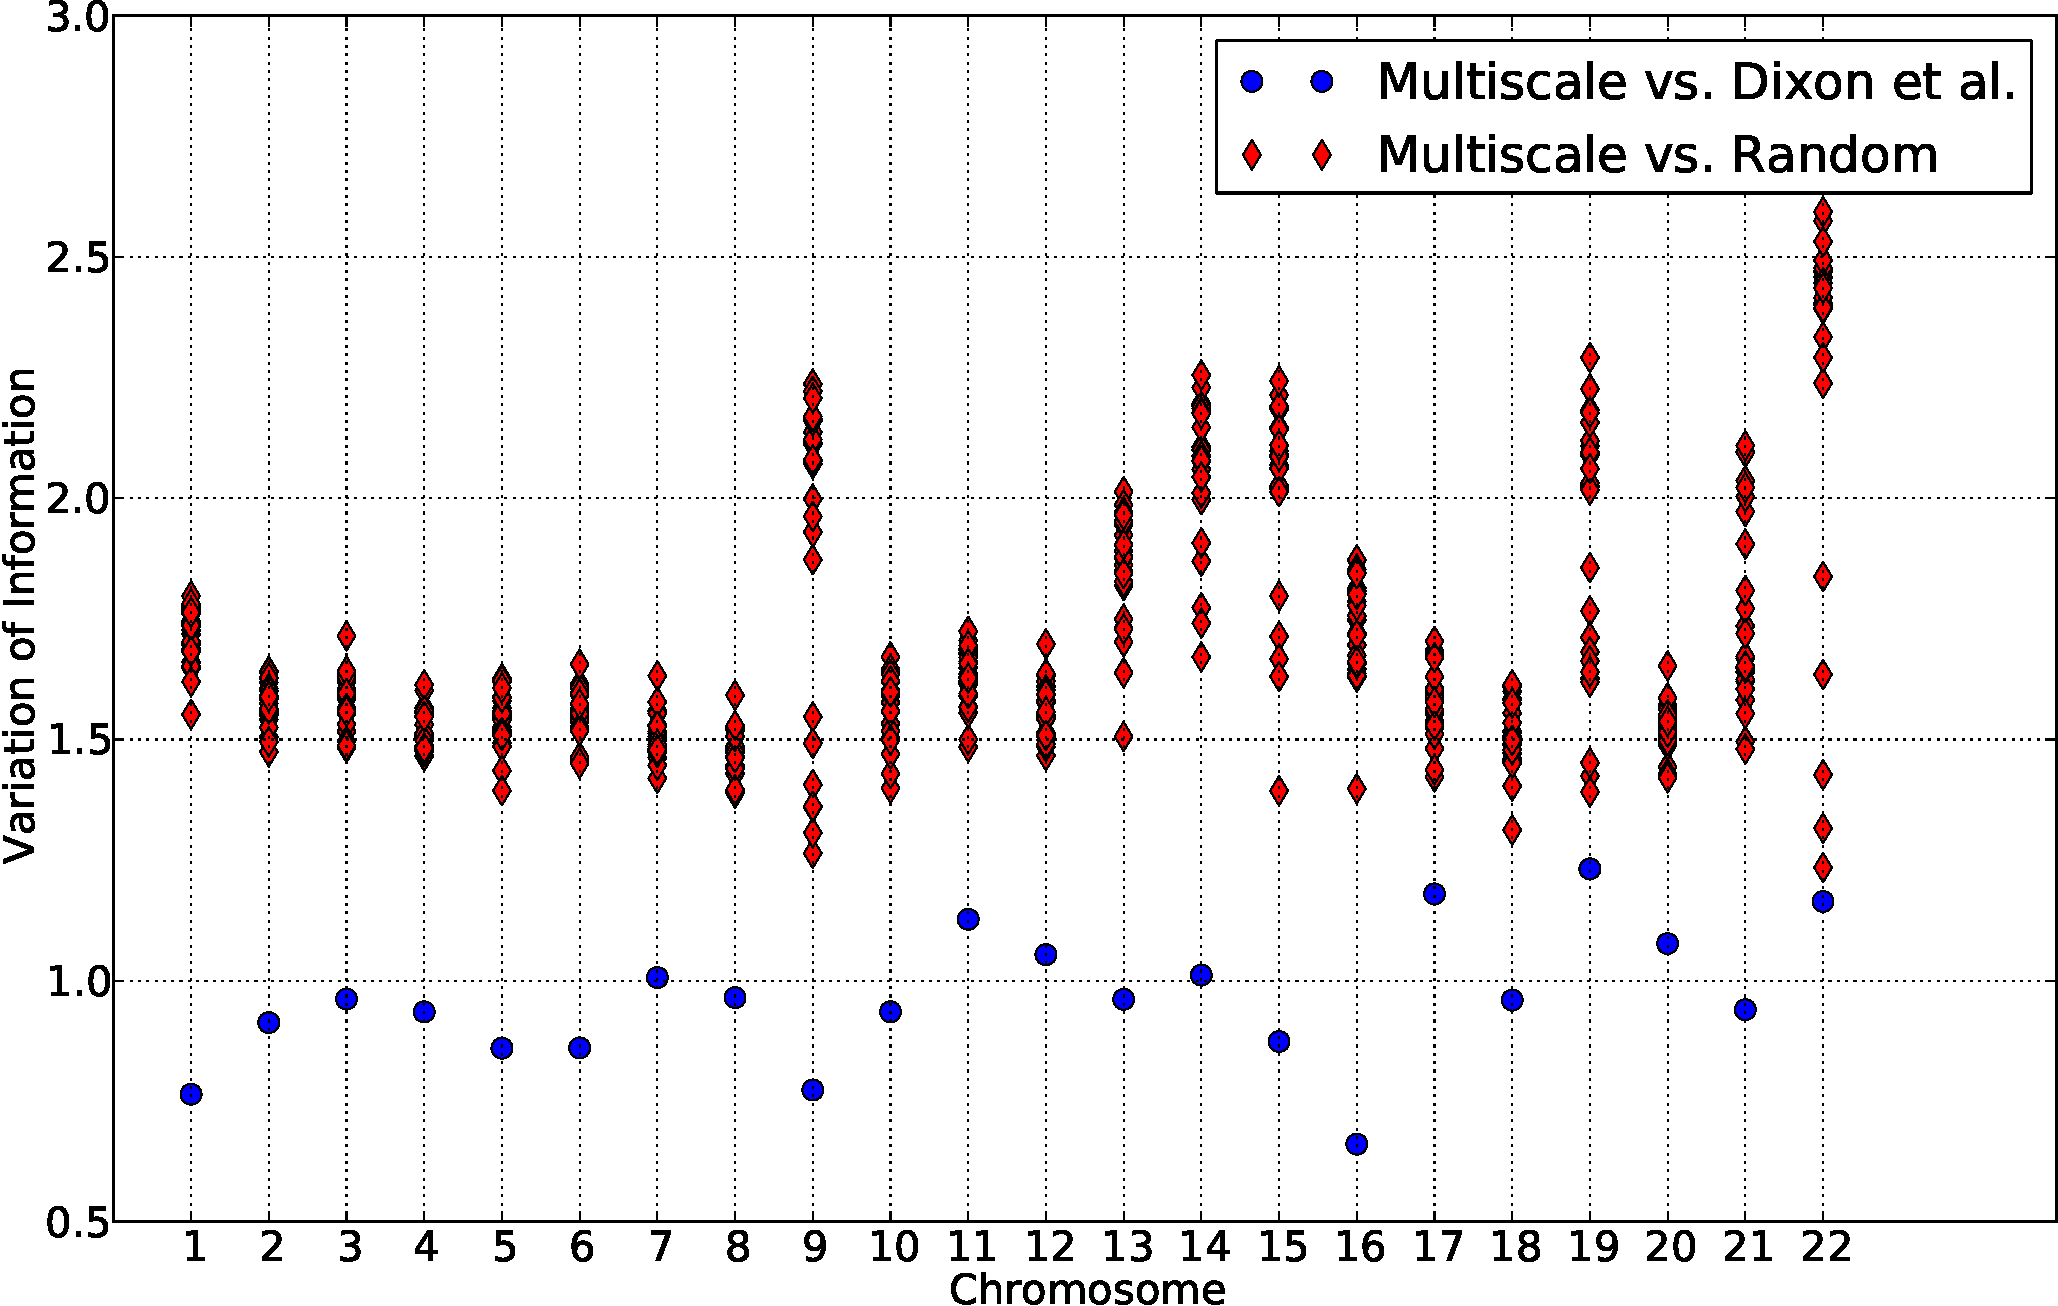
\includegraphics[width=.9\linewidth]{figures/UsVsBingVI}
    \end{center}
    \caption{\textbf{Comparison of Dixon et al.'s domain set} with the multiscale consensus set for chromosomes 1--22 ($x$-axis). We used the variation of information (VI) ($y$-axis) to compute distances between domain sets for the multiscale consensus set vs. Dixon et al. (blue dots) and the multiscale consensus vs. randomly shuffled domains (red diamonds).}
    \label{fig:consensus_agreement}
  \end{figure}

  At higher resolutions, domains identified by our algorithm are smaller than those reported by Dixon et al. (Figure~\ref{subfig:sizeCount}). As the resolution parameter decreases to 0.0, the average size of the domains increases  (see Figure~\ref{fig:dom_size} for results for chromosome 1 on the IMR90 human fibroblast cells). As domains expand to cover more and more of the chromosome, the similarity to the domains identified by Dixon et al.~\cite{Dixon2012} also increases (Figure~\ref{subfig:dixonSim}). We calculate the Jaccard similarity between two sets of domains $D$ and $D'$ as $J(D, D') = N_{11} / (N_{11} + N_{01} + N_{10})$ where the quantities $N_{11}$, $N_{01}$, and $N_{10}$ are the number of 3C fragments that are in a domain in both sets $D$ and $D'$, the number of fragments that are in a domain in $D'$, but not in $D$, and the number of fragments that are in a domain in $D$, but not $D'$, respectively (light blue in Figure~\ref{subfig:dixonSim}). The composition of the domains, however, is different as is captured by the variation of information (red in Fig.~\ref{subfig:dixonSim}). Overall, we identify domains that cover similar regions of the chromosome (Figures~\ref{fig:armatus:size-freq},~\ref{fig:armatus:freq-distr}), yet differ in their size distribution and genomic positions.

  We use the algorithm described in section~\ref{consensusalg} to obtain a consensus set of domains $D_c$ persistent across resolutions. We construct the set $\Gamma$ by defining the range of our scale parameter to be $[0, \gamma_\textrm{max}]$ and incrementing $\gamma$ in steps of 0.05. In order to more directly compare with previous results, we set $\gamma_{\max}=0.5$ for human and $0.25$ for mouse since these are the scales at which the maximum domain sizes in Dixon et al.'s sets match the maximum domain sizes in our sets.

  Our consensus domain set agrees with the Dixon et al. domains better than with a randomized set of domains adhering to the same domain and non-domain length distributions (Figure~\ref{fig:consensus_agreement}). Our primary motivation in comparing to randomized sets of domains is to provide a baseline that we can use to contrast our set of domains with Dixon et al. Comparing to a set of random domains also helps to verify that our observations are due to the observed sequence of domains and not the distribution of domain lengths. To shuffle Dixon's domains, we record the length of every domain and non-domain region, and then shuffle these lengths to obtain a randomized order of domains and non-domains across the chromosome.  The fact that variation of information is lower between consensus domains and domains reported by Dixon et al. demonstrates that, though the approaches find substantially different sets of topological domains, they still agree significantly more than one would expect by chance.

  %%%%%%%%%%%%%%%%%%%%%%%%%%%%%%%%%%%%%%%%%%%%%
  %
  %%%%%%%%%%%%%%%%%%%%%%%%%%%%%%%%%%%%%%%%%%%%%
  \subsection{Enrichment of CTCF and histone modifications near boundaries}
  \label{sec:Enrichment}

  We assess the enrichment of transcription factor CTCF and histone modifications H3K4me3 and H3K27AC within the inter-domain regions induced by the consensus domains. These enrichments provide evidence that the boundary regions between topological domains correlate with genomic regions that act as insulators and barriers, suggesting that the topological domains may play a role in controlling transcription in mammalian genomes~\cite{Dixon2012}.

  Figure~\ref{fig:enrichment} illustrates the enrichment of insulator or barrier-like elements in domain boundaries in both the human fibroblast (IMR90) and mouse embryonic stem cell (mESC) lines.  Specifically, we observe that
  the boundaries between consensus domains are significantly enriched for all of the transcription factors and histone marks we consider.  In certain cases --- specifically in the case of CTCF --- we notice that the CTCF binding signals peak more sharply in the boundaries between the domains we discover than in the boundaries between the domains of Dixon et al.

  \begin{figure}[ht]
  %
  \begin{center}
  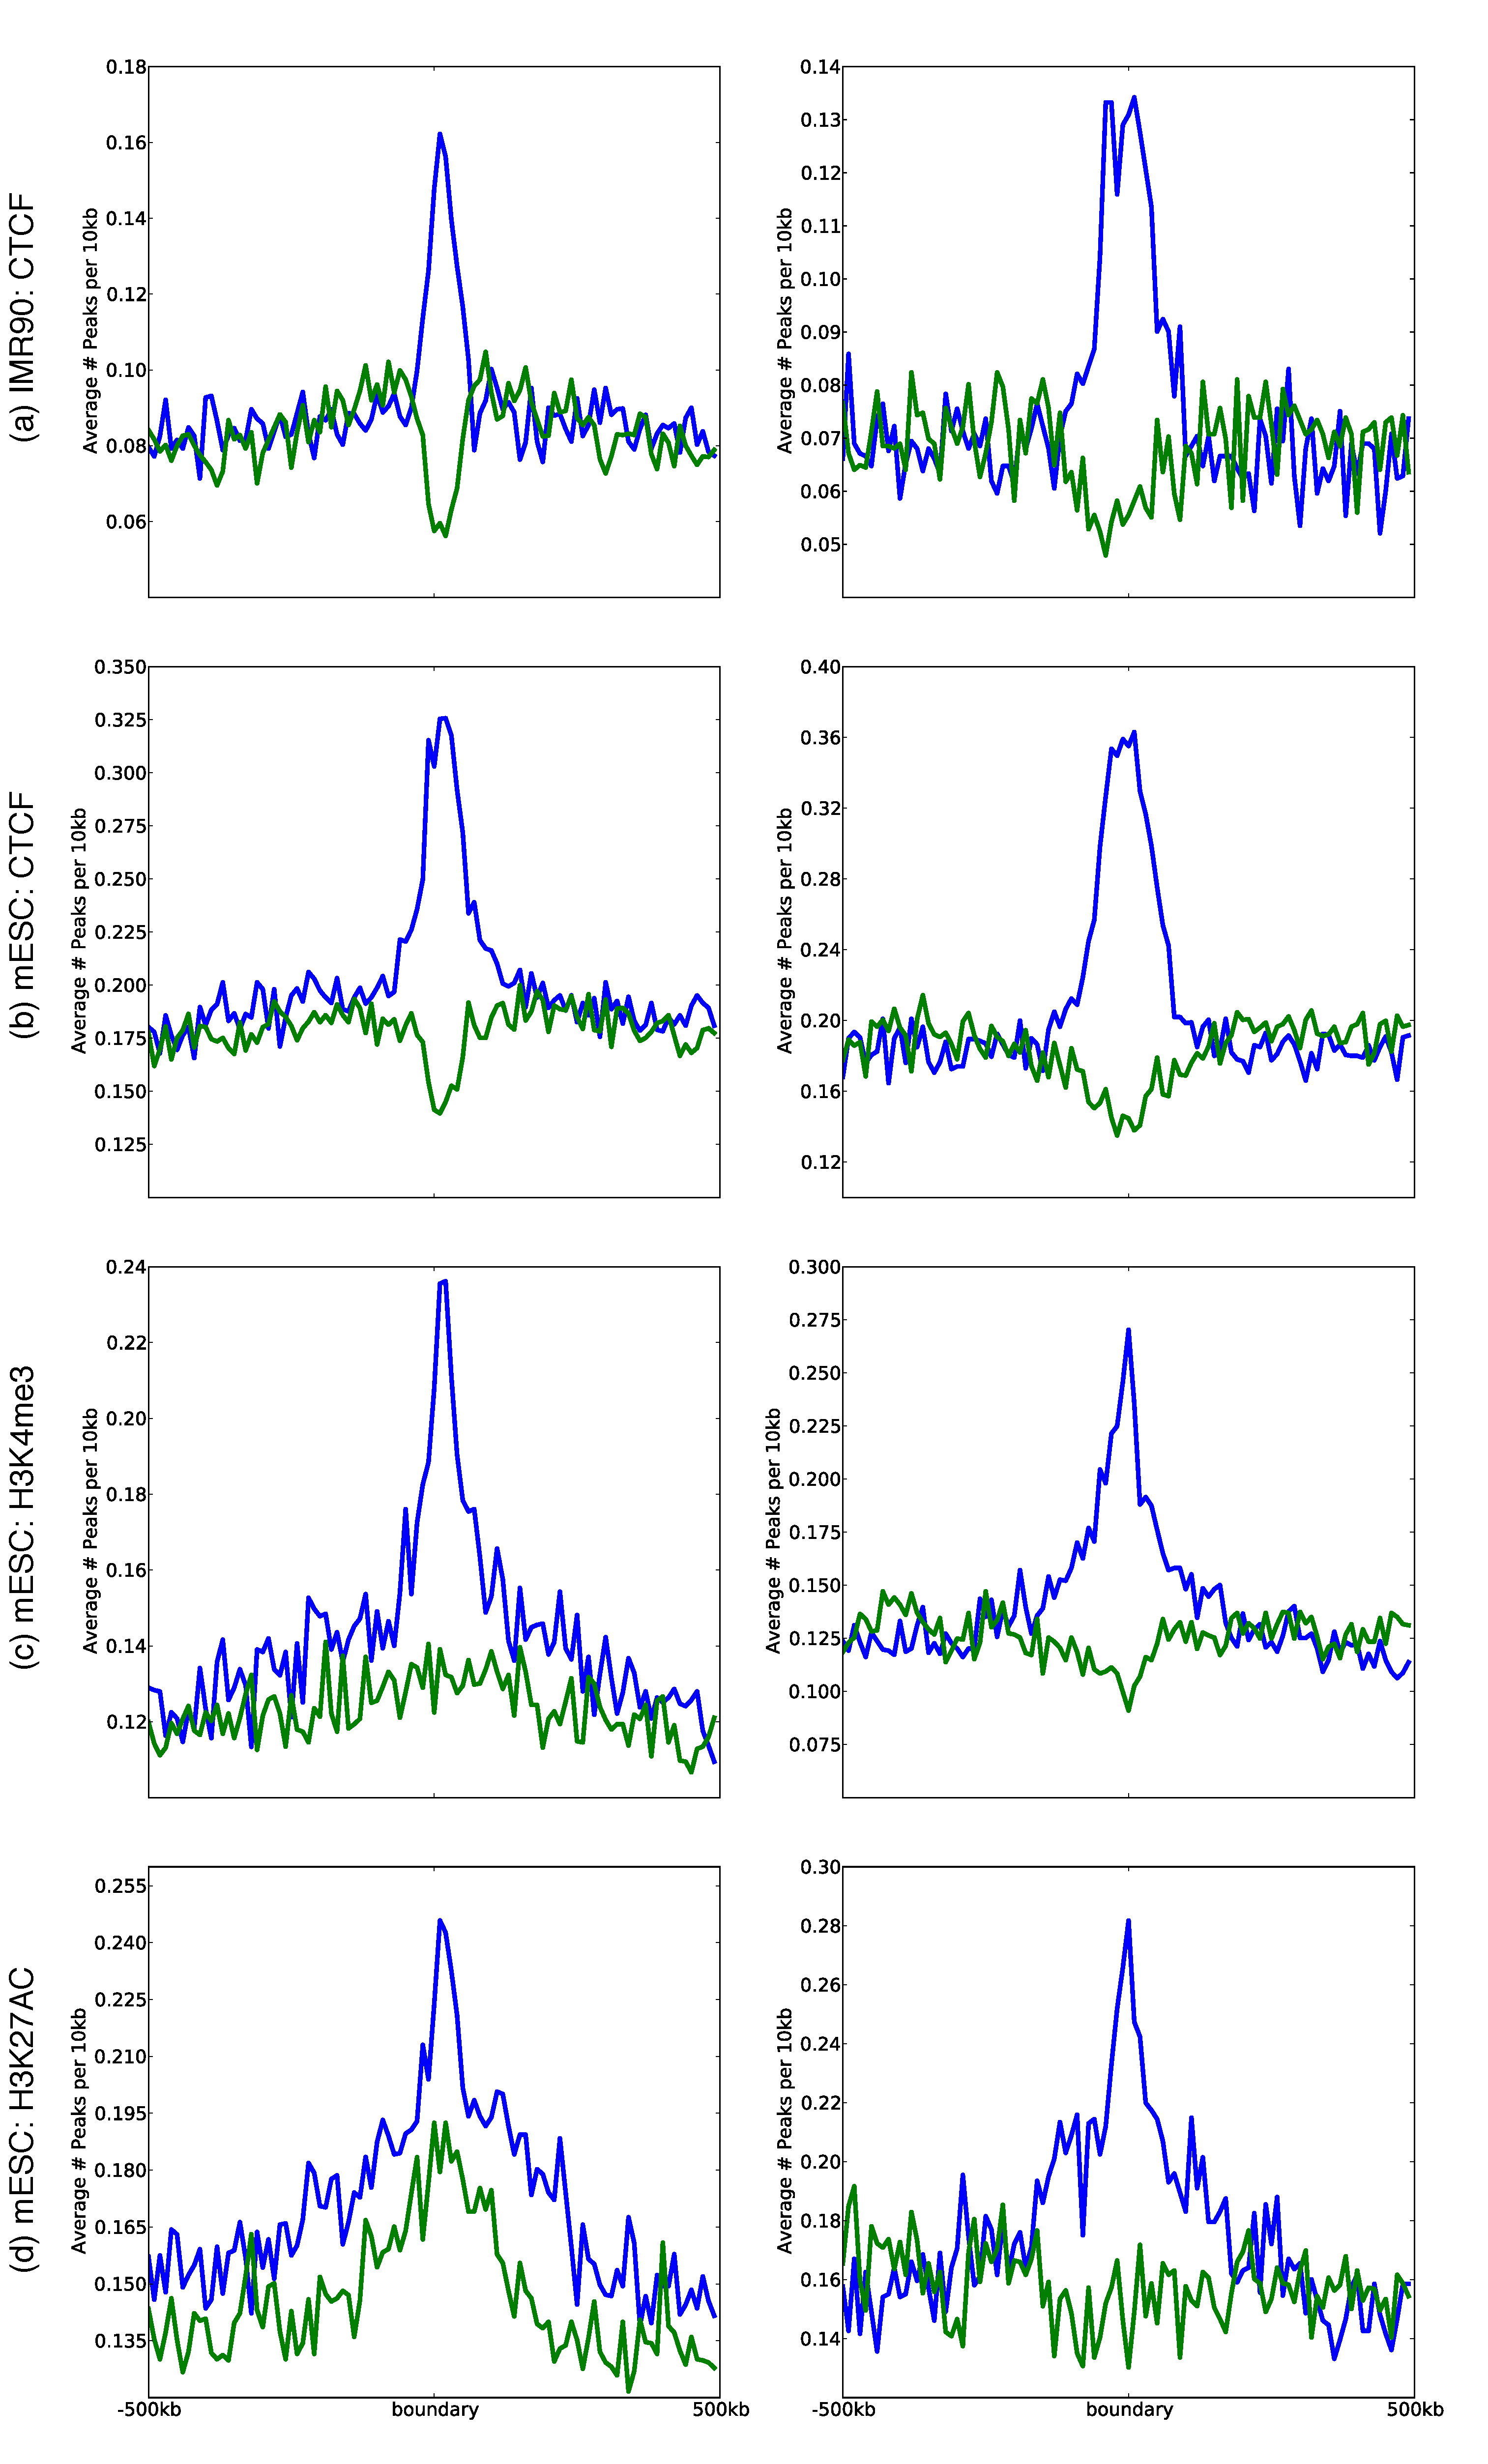
\includegraphics[width=0.73\textwidth]{figures/fig6_combined_rotated}
  % \subfigure[IMR90: CTCF]{
  % \includegraphics[width=2.1in]{IMR90_CTCF_Ours}
  % \includegraphics[width=2.1in]{IMR90_CTCF_Bingy}
  % \label{fig:CTCF}
  % }
  % %
  % \subfigure[mESC: CTCF]{
  % \includegraphics[width=2.1in]{mESC_CTCF_Ours}
  % \includegraphics[width=2.1in]{mESC_CTCF_Bingy}
  % \label{fig:mESC_CTCF}
  % }
  % %
  % \subfigure[mESC: H3K4me3]{
  % \includegraphics[width=2.1in]{mESC_H3K4me3_Ours}
  % \includegraphics[width=2.1in]{mESC_H3K4me3_Bingy}
  % \label{fig:H3K4me3}
  % }
  % %
  % \subfigure[mESC: H3K27AC]{
  % \includegraphics[width=2.1in]{mESC_H3K27AC_Ours}
  % \includegraphics[width=2.1in]{mESC_H3K27AC_Bingy}
  % \label{fig:H3K27AC}
  % }
  \caption{\textbf{Enrichment of binding CTCF binding} (a) in IMR90 and (b) in mESC and histone modifications (c), (d) in mESC around domain boundaries for our consensus set of persistent domains (left, blue), and for those identified by Dixon et al. (right, blue).  Green lines represent the presence of CTCF at the midpoint of the topological domains.}
  \label{fig:enrichment}
  \end{center}
  \end{figure}


  \begin{table}[b]
  \centering
  \caption{\textbf{Domain enrichment.} Each table entry is of the form $\frac{e}{t} \approx r$ where $e$ is the number of elements containing $\ge 1$ of CTCF and histone modifications, $t$ is the total number of elements and $r$ is the approximate ratio $e/t$.  Our method produces more domains,
  and hence more boundaries, than that of Dixon et al.~\cite{Dixon2012}.  However, relative to Dixon et al., our domains are depleted for peaks of interest, while our boundaries are significantly enriched
  for such peaks.}
  %Our method tends to produce ($1.6$---$2.3$ times) more domains than that of Dixon et al.~\cite{Dixon2012}.  However, while the domains produced by both methods contain at least peak for the different chromatin factors we consider in roughly the same proportion, the boundaries between our domains contain at least one peak for these factors about twice as frequently as the boundaries between the domains of Dixon et al.}
  \label{tab:differentalEnrichment}
  \scriptsize
  \begin{tabular}{lc@{\hskip 15pt}c@{\hskip 5pt}|@{\hskip 5pt}c@{\hskip 15pt}c@{\hskip 15pt}c}
  \toprule
  %& \multicolumn{3}{r}{Ratio: (current method / \cite{Dixon2012})} \\
  %\cmidrule(r){2-4}
  Signal & Domains (\cite{Dixon2012}) & Domains (Ours) & Boundaries (\cite{Dixon2012}) & Boundaries (Ours) \\
  %       & Domains w/ $\ge 1$ peak        & w/ $\ge 1$ peak & w/ $\ge 1$ peak \\
  \midrule
  CTCF (IMR90)   & $\frac{2050}{2234}\approx0.92$ & $\frac{3092}{5365}\approx0.58$ & $\frac{423}{2136}\approx0.20$ & $\frac{2126}{4861}\approx0.44$ \\[0.5em]
  CTCF (mESC)    & $\frac{2057}{2066}\approx1.00$ & $\frac{2500}{3578}\approx0.70$ & $\frac{654}{2006}\approx0.33$ & $\frac{2258}{3122}\approx0.72$ \\[0.5em]
  H3K4me3 (mESC) & $\frac{2019}{2066}\approx0.98$ & $\frac{2362}{3578}\approx0.66$ & $\frac{600}{2006}\approx0.30$ & $\frac{1738}{3122}\approx0.60$ \\[0.5em]
  H3K27AC (mESC) & $\frac{1922}{2066}\approx0.93$ & $\frac{2254}{3578}\approx0.63$ & $\frac{458}{2006}\approx0.23$ & $\frac{1342}{3122}\approx0.43$ \\
  \bottomrule
  \end{tabular}
  \end{table}
  % \vspace{-25px}

  We also observe that, when compared with the domain boundaries predicted by Dixon et al., our boundaries more often contain insulator or barrier-like elements (see Table~\ref{tab:differentalEnrichment}). Specifically, we normalize for the fact that we identify approximately twice as many domains as Dixon et al., and generally observe a two-fold enrichment in the fraction of boundaries containing
  peaks for CTCF markers. This suggests that structural boundaries identified by our method are more closely tied to functional sites which serve as barriers to long-range regulation. We also observe a depletion of insulator CTCF elements within our domains when compared to the domains of Dixon et al.  This observation is consistent with the assumption that transcriptional regulation is more active within spatially proximate domains since there are fewer elements blocking regulation within these domains.  Table~\ref{tab:differentalEnrichment} also shows similar patterns for histone modifications which suggests that our domain boundaries are enriched for functional markers of gene regulation.

\section{Discussion and Conclusions}

  In this chapter, we introduce an algorithm to identify topological domains in chromatin using interaction matrices from recent high-throughput chromosome conformation capture experiments.  Our algorithm produces domains that display much higher interaction frequencies within the domains than in-between domains (Figure~\ref{fig:armatus:freq-distr}) and for which the boundaries between these domains exhibit substantial enrichment for several known insulator and barrier-like elements (Figure~\ref{fig:enrichment}).  To identify these domains, we use a multiscale approach which finds domains at various size scales.  %To obtain a single set of domains from this rich ensemble, e extract a non-overlapping set of consensus domains that are most persistent across multiple length scales.
  We define a consensus set to be a set of domains that persist across multiple resolutions and give an efficient algorithm that finds such a set optimally.

  % -- Practical running time
  The method for discovering topological domains that we have introduced is practical for existing datasets.  Our implementation is able to compute the consensus set of domains for the human fibroblast cell line and extract the consensus set in under 40 minutes when run on a personal computer with 2.3GHz Intel Core i5 processor and 8Gb of RAM.


  Our method is particularly appealing in that it requires only a single user-specified parameter $\gamma_{\text{max}}$. It uses a score function that encodes the quality of putative domains in an intuitive manner based on their local density of interactions.  Variations of the scoring function in~(\ref{quality}), for example, by median centering rather than mean centering, can be explored to test the robustness of the enrichments described here. For our experiments, the parameter $\gamma_{\max}$ was set based on the maximum domain sizes observed in Dixon et. al's experiments so that we could easily compare our domains to theirs.  This parameter can also be set intrinsically from properties of the Hi-C interaction matrices.  For example, we observe similar enrichments in both human and mouse when we set $\gamma_{\max}$ to be the smallest $\gamma \in \Gamma$ such that the median domain size is $>$80kbp (two consecutive Hi-C fragments at a resolution of 40kbp). This is a reasonable assumption since domains consisting of just one or two fragments do not capture higher-order spatial relationships (e.g. triad closure) and interaction frequencies between adjacent fragments are likely large by chance~\cite{LiebAid2009}.  We also compared the fraction of the genome covered by domains identified by Dixon et al. vs. the domains obtained from our method at various resolutions.  Dixon et al.'s domains cover 85\% of the genome while our sets tend to cover less of the genome ($\approx$ 65\% for a resolution which results in the same number of domains as those of Dixon et al.).  The fact that our domain boundaries are more enriched for CTCF sites indicates that our smaller, more dense domains may be more desirable from the perspective of genome function.

  The dense, functionally-enriched domains discovered by our algorithm provide strong evidence that alternative chromatin domains exist and that a single length scale is insufficient to capture the hierarchical and overlapping domain structure visible in heat maps of 3C interaction matrices. Our method explicitly incorporates the desirable properties of domain density and persistence across scales into objectives that maximize each and uncovers a new view of domain organization in mammalian genomes that warrants further investigation.


%  XXX: Russell -- I could imagine building in a model complexity penalty to choose the best-supported scale and maybe even allow that to vary across genome. would something like that be feasible?

  % addressing Russell's comment on model complexity for domains

  % Developing a statistical model for domain generation would allow to select a set of the most consistent domains given an interaction matrix in a more principled manner.
  An interesting extension to the problem of finding consistent domains would be to build a comprehensive statistical model for domain generation. Such a model would allow to evaluate the likelihood of a particular set of domains at a given scale and guide the selection of the most likely set by minimizing model complexity. Iqbal and Patro~\cite{IqbalDomains}, as well as Weinreb and Raphael~\cite{WeinrebDomains} have recently presented two domain models that choose a set of domains across scales by maximizing such global domain quality criteria.



%%%%%%%%%%%%%%%%%%%%%%%%%%%%%%%%%%%%%%%%%%%%%%%%%%%%%%%%%%%%%%%%%%%%%%%%%%%%%%%
%%%%%%%%%%%%%%%%%%%%%%%%%%%%%%%%%%%%%%%%%%%%%%%%%%%%%%%%%%%%%%%%%%%%%%%%%%%%%%%
%%
%%
%%
%% Part 2 -- high-level structure and compression
%%
%%
%%%%%%%%%%%%%%%%%%%%%%%%%%%%%%%%%%%%%%%%%%%%%%%%%%%%%%%%%%%%%%%%%%%%%%%%%%%%%%%
%%%%%%%%%%%%%%%%%%%%%%%%%%%%%%%%%%%%%%%%%%%%%%%%%%%%%%%%%%%%%%%%%%%%%%%%%%%%%%%
\part{Compression approaches for sequencing and alignment data}
\label{part:compress}


%%%%%%%%%%%%%%%%%%%%%%%%%%%%%%%%%%%%%%%%%%%%%%%%%%%%%%%%%%%%%%%%%%%%%%%%%%%%%%%
%%%%%%%%%%%%%%%%%%%%%%%%%%%%%%%%%%%%%%%%%%%%%%%%%%%%%%%%%%%%%%%%%%%%%%%%%%%%%%%
%
%
% de novo sequence compression

%   -- can compress similar genomes against each other (\cite{reference})
%   -- suggests there might be a grammar describing sequence

%   -- used grammar finder on concatenated reads -- results not promising. grammar size XXXX, compressed size XXX

%   -- using kmer dictionaries
%     -- building kmer dictionaries: single K
%     -- multiple K
%     -- mixing various K lengths

%   -- optimal string parsing given a dictionary
%     -- filling in the gaps
%     -- allowing up to 2 substitutions

%   -- performance on some related data: 
%     -- size of dictionary
%     -- encoding self with your dictionary
%     -- cross-encoding related data

%     -- dictionary size on the single cell RNA-seq
%       -- dicitonary size keeps growing
%       -- kmer set overlaps between the sets is small
%       -- most kmers are not even in the transcriptome
%       -- but they do align well to the genome
%       -- CONCLUSION: too much variability, a single error , plus read boundaries matter

%   -- conclusions
%     -- dictionary coders like SCALCE and MINCE replace whole swathes of seuqence
%     -- kmer dictionary will always spend bits when seeing the same kmer
%     -- error rates and read boundaries do no allow for efficient shared dictionary construction based on kmers
%
%%%%%%%%%%%%%%%%%%%%%%%%%%%%%%%%%%%%%%%%%%%%%%%%%%%%%%%%%%%%%%%%%%%%%%%%%%%%%%%
%%%%%%%%%%%%%%%%%%%%%%%%%%%%%%%%%%%%%%%%%%%%%%%%%%%%%%%%%%%%%%%%%%%%%%%%%%%%%%%

%%%%%%%%%%%%%%%%%%%%%%%%%%%%%%%%%%%%%%%%%%%%%%%%%%%%%%%%%%%%%%%%%%%%%%%%%%%%%%%
%%%%%%%%%%%%%%%%%%%%%%%%%%%%%%%%%%%%%%%%%%%%%%%%%%%%%%%%%%%%%%%%%%%%%%%%%%%%%%%
%%
%%
%% Huffmer and Referee -- compression projects
%%
%%
%%%%%%%%%%%%%%%%%%%%%%%%%%%%%%%%%%%%%%%%%%%%%%%%%%%%%%%%%%%%%%%%%%%%%%%%%%%%%%%
%%%%%%%%%%%%%%%%%%%%%%%%%%%%%%%%%%%%%%%%%%%%%%%%%%%%%%%%%%%%%%%%%%%%%%%%%%%%%%%
\chapter{De novo sequence compression with shared dictionaries}


Previous chapters address visualization and analysis challenges presented by data that has already been processed: networks constructed from raw data, annotations, and quantified abundances of histone modifications. However, as we go back to the tasks involving raw data, the data size and complexity increase to the extent that not only visualization, but even storage, dissemination, and basic analysis of such data become a computational challenge. For example, chromatin interaction data for a human chromosome 1 used in the previous chapter fits on disk withing 134Mb, however, building required merging and aligning sequencing data from several replicates that in total added up to 70Gb. Large sequencing data warehouses, e.g. Sequence Read Archive (SRA)~\cite{SRA}, and labs with modest computational resources alike face these computational challenges due to the explosion in the amount of generated sequencing data.

Commonplace compression tools like gzip that is based on Lempel-Ziv original paper~\cite{LempelZiv77}, and bzip2 that leverages Burrow-Wheeler transform~\cite{BWTransform} are often used to compress large read datasets, however, they do not exploit the specific nature of sequencing reads: its small alphabet, highly repetitive subsequences, higher error rates as compared to a natural language, reverse complementarity, and the fact that sequence may originate from a well-annotated known genome. SRA data format is commonly used to store FASTQ files which include the reads themselves and additional base quality information, however, even the specialized compression methods easily outperform this compression technique~\cite{SeqSqueeze}.

In this chapter, we explore the idea of shared information --- information that is common to many sequencing data. The nucleotide bases are universal to all DNA and, therefore, are one example of such shared information. Indeed, 2-bit sequence encoding is commonly used to encode sequence more efficiently. On the other hand, sequence is non-random and may have a large scale structure akin to the grammar of the human language. We explore a variant of shared information we call a \textit{shared dictionary} --- a collection of frequent subsequences that lends itself to optimal Huffman coding. We consider several algorithms for building the dictionary and derive an optimal algorithm for encoding an input sequence given a dictionary. Shared dictionaries are competitive with state of the art tools when we assume that the cost of transmitting the dictionary could be amortized over multiple downloads of the data it encodes. However, we observe that encoding a sequence with a dictionary that was trained on a different data decreases the compression rates. Further, we discover that building a dictionary based on frequent substrings across multiple datasets is a difficult problem due to natural variation in sequence, sequencing errors, and the boundary effects introduced by the read length.


%%%%%%%%%%%%%%%%%%%%%%%%%%%%%%%%%%%%%%%%%%%%%%%%%%%%%%%%%%%%%%%%%%%%%%%%%%%%%%%
\section{Background}


The amount of sequencing data stored in the Sequence Read Archive (SRA) is currently at 775337Gb and growing~\cite{SRA} --- this growth of generated data demands novel scalable approaches to its storage and transmission. It is also crucial that compression approaches are \textit{functional}, i.e.\@ that analyses could be run on the dataset in its compressed format without having to fully reconstruct it. 


In the area of sequence compression, two prevalent approaches exist: the \textit{reference-based} (discussed in the next chapter) and \textit{reference-free}, or \textit{de novo}, methods. \textit{De novo} compression operates on raw sequencing reads, FASTA, or FASTQ files as input and focuses on ways to compress sequence~\cite{Mince,PathEncode,Rozov2014}, quality values~\cite{SeqSqueeze,KmerQuals,JaninQuals}, or both~\cite{GSQZ,Sahinalp2012}. 
% to address Russell's later comment on why seq compression is different from qual compression
Sequence and quality value compression are usually addressed separately due to inherent differences between the two types of data: while reads capture a non-random sequence of nucleotides with its repretitive regions, homologs, variations between coding and non-coding regions, the quality values encode the state of the sequencing machine as it was at the time of observing these nucleotides which results in different alphabets for the two data sources and different substring distributions. In this chapter, we focus on sequence compression exclusively and consider quality values compression in the later sections.

Tools like SCALCE~\cite{Sahinalp2012} and Mince~\cite{Mince} take the approach of grouping the reads based on their similarity allowing the downstream general-purpose compression tools to build better dictionary encodings. Rozov \etal~\cite{Rozov2014} and recent work by Kingsford and Patro~\cite{PathEncode} use an available reference sequence to inform their compression algorithm without explicitly aligning reads to it. Quip~\cite{Jones2012} takes a step closer to reference-based approach by creating contigs from a subset of data and encoding the rest of the reads relative to that lightweight assembly. De novo compression tools compress sequence down to 3-10\% of its original size at reasonable speeds~\cite{Deorowicz2013}, however, most tools require that the dataset is completely decompressed before it could be used for downstream analyses.


%%%%%%%%%%%%%%%%%%%%%%%%%%%%%%%%%%%%%%%%%%%%%%%%%%%%%%%%
\section{Compressing sequence with standard command-line tools}

  The repetitive nature of sequencing data suggests that dictionary-based coders, like the commonplace command-line tools \texttt{gzip}, \texttt{bzip}, and \texttt{plzip}, should be able to compress collections of reads reasonably well. Indeed, general purpose compressors offer a 3x-9x reduction in size. However, the order of the reads in a file is arbitrary and simply reordering the reads improves compression ratios vastly: for data shown in Table~\ref{tab:compression:clt}, the size of compressed data was reduced by up to 5 times after running \texttt{sort} utility on the original reads. Additionally, since the reads are derived from DNA and could represent the sequence in the forward or the reverse direction, the read and its reverse compliment are considered equivalent. Choosing to transform some of the reads to their reverse complements increases read homogeneity and can further improve compression, although finding such optimal read ordering and directionality turns out to be a hard problem~\cite{PatroLCPRC}.

  \begin{table}[ht]
    \centering
    \subfigure[Reads]{
      \begin{tabular}{l r r r r}
      \toprule
      Dataset & Seq. size & gzip & bzip & plzip \\
      \midrule
      % SRR635193\_1 & 448028499 & 388127969 & 298812728 \\
      % SRR519063\_1 & 275904124 & 171751232 & 149554794 \\
      % ERR233214\_1 & 208082597 & 189126709 & 119758802 \\
      SRR635193\_1 & 1430 & 427 & 370 & 284 \\
      SRR519063\_1 & 1338 & 263 & 163 & 142 \\
      ERR233214\_1 & 673 & 198 & 180 & 114 \\
      \bottomrule
      \end{tabular}
      \label{fig:compression:unordered}
    }
    \subfigure[Reordered reads]{
      \begin{tabular}{l r r r}
      \toprule
      Dataset & gzip & bzip & plzip \\
      \midrule
      SRR635193\_1 & 166 & 195 & 128 \\
      SRR519063\_1 & 43 & 48 & 28 \\
      ERR233214\_1 & 95 & 121 & 64 \\
      \bottomrule
      \end{tabular}
      \label{fig:compression:reordered}
    }
    \caption{\textbf{Performance of command-line compression tools on sequencing reads.} Reordering the reads improves reads compression by up to 5 times. Sizes shown are in megabytes.}
    \label{tab:compression:clt}
  \end{table}

%%%%%%%%%%%%%%%%%%%%%%%%%%%%%%%%%%%%%%%%%%%%%%%%%%%%%%%%
% \section{Applying grammar-based sequence encoding to reads}

    % -- can compress similar genomes against each other (\cite{reference})

    % -- suggests there might be a grammar describing sequence

    % -- used grammar finder on concatenated reads -- results not promising. grammar size XXXX, compressed size XXX

    % XXX what if trained the grammar on the genome, then used the learned grammar to compress reads for that organism?

%%%%%%%%%%%%%%%%%%%%%%%%%%%%%%%%%%%%%%%%%%%%%%%%%%%%%%%%
\section{Building a dictionary of information shared across sets of sequencing reads}

  % additional definitions
  \newcommand{\seq}{\mathcal{S}\xspace}
  \newcommand{\compseq}{\widetilde{\mathcal{S}}\xspace}

  % what is shared information.
  

  We investigate compression methods that rely on a paradigm of \textit{shared information}. For example, given multiple human RNA-seq datasets $\mathcal{ S}_1, \mathcal{ S}_2, \ldots$, the information encoded in the sequencing reads of each $\mathcal{ S}_i$ is highly redundant across all $\mathcal{S}_i$.  These datasets would only differ due to genomic variations between individuals and the number of copies for the expressed genes, however, most of the sequence data would be repeated. We seek a method that can identify and efficiently compress data shared across multiple datasets. When a large genomic center distributes compressed data $\mathcal{\widetilde S}_i$, the dictionary $D$ of information shared among all $\mathcal{S}_i$ need only be downloaded once and its cost would be amortized over multiple transmissions of $\mathcal{\widetilde S}_1$, $\mathcal{\widetilde S}_2$, \ldots.

  Given the input datasets $\mathcal{ S}_1, \mathcal{ S}_2, \ldots$, we seek such dictionary $D$ that compression ratio $(\sum_i |\compseq_i| + D) / \sum_i |\seq_i|$ is minimized over multiple transmissions of the compressed sequences $\compseq_i$. Alternatively, we may want to construct multiple dictionaries $D_1, \ldots, D_\delta$ such that for each $\seq_i$, parts of the original sequence are best compressed by one of these dictionaries $D_j$. We will then seek a collection of dictionaries $D_1, \ldots, D_\delta$ and a matching function $f(\seq_i \to D_j)$ such that the compression ratio $(\sum_i |\compseq_i| + \sum_j D_j) / \sum_i |\seq_i|$ is minimized and the function $f(D_j) \to s$ efficiently maps parts of the original sequence $\seq_i$ to dictionary $D_j$ that would provide the best compression.

%%%%%%%%%%%%%%%%%%%%%%%%%%%%%%%%%%%%%%%%%%%%%%%%%%%%%%%%
\subsection{Building efficient kmer-based dictionaries}

We assume that original sequence $\seq$ is a concatenation of reads $\seq = \{s_1, s_2, \ldots \}$, that sequencing reads in $\seq$ can only contain four distinct symbols representing nucleotides (A, C, T, G) and that all reads in $\seq$ have the same length. A \textit{kmer} $d$ of length $k$ is a sequence of $k$ nucleotides that appears somewhere in $\seq$. 
% Kmer composition can be seen as a footprint of a specific collection of reads: distribution of 24-mers for RNA-seq dataset is qualitatively different from a distribution of 24-mers for a DNA dataset; kmers can be used to distinguish between coding and non-coding DNA~\cite{genes}... 
Certain kmers tend appear much more frequently in $\seq$ making a distribution of kmer occurrences highly skewed and amenable to efficient entropy-based encodings, \eg~with Huffman codes.

Huffman coding~\cite{Huffman1952} is a lossless data compression technique that assigns shorter codes to symbols with higher frequency and guarantees that codes are prefix-free (no codeword is a prefix of some other codeword) allowing for unambigous decoding. 
Usually, Huffman coding is applied to compress natural text where the codes are built for individual letters of an alphabet or words. Here, we propose to use kmers as input symbols for Huffman coding.

Since Huffman codes assume that symbols $d_i$ do not overlap, we only consider non-overlapping kmers for inclusion in the dictionary. Kmer counting produces a distribution $\mathcal{F} = \{(f_1, d_1), (f_2, d_2), \ldots \}$ where $f_i \in \mathbb{N}$ represents the number of times a kmer $d_i$ was seen in $\seq$. We then generate Huffman codes $C = \{ c_i | d_i \in D \}$ based on $\mathcal{F}$ and substitute kmers $d_i$ in $\seq$ with their corresponding binary codes $c_i$. This dictionary construction procedure guarantees that every base in $\seq$ is covered by a kmer in $D$ and ensures that $D$ is optimal for a given ordering of reads in $\seq$.

% This approach was able to reduce the file size to a factor of 1/7th of the original size and, in certain instances, even outperformed state of the art tools (see Figure~\ref{fig:denovocompr:varyK}).

  % \subsection{Building dictionaries to maximize coverage}

  % We first build the dictionary on a sequence $\seq$ by concatenating the reads and then counting non-overlapping kmers of uniform length $k$ on $\seq$. 


  \begin{figure}[ht]
    \centering
    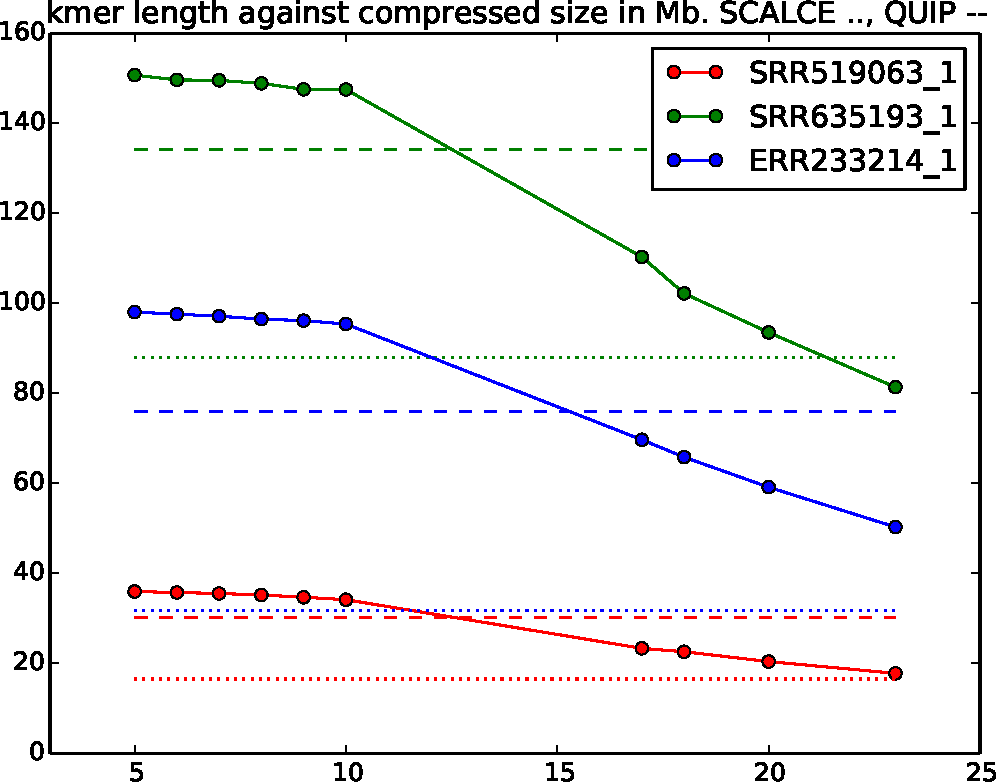
\includegraphics[width=0.7\linewidth]{figures/vary-k-fullfile-singleline}
    \caption{\textbf{Optimal dictionary construction on a string of concatenated reads.} Increasing kmer length improves compression performance. Dictionary size not included in the size of the compressed data. Dashed lines represent the size of the file compressed with Quip~\cite{Jones2012} and dotted lines represent the size of the file compressed with SCALCE~\cite{Sahinalp2012}.}
    \label{fig:denovocompr:varyK}
  \end{figure}

  We evaluate this strategy on three diverse datasets: human RNA-seq (SRR635193), \textit{P. aeruginosa} RNA-seq (SRR519063), and whole genome sequencing of the same bacterium (ERR233214, see Figure~\ref{fig:denovocompr:varyK}). We observe that as $k$ increases, naive dictionary encoding improves. This approach was able to reduce the file size to a factor of 1/7th of the original size and, in certain instances, even outperformed state of the art tools.

  %%%%%%%%%%%%%%%%%%%%%%%%%%%%%%%%%%%%%%%%%%%%%%%%%%%%%%%%
  \subsection{Building dictionaries to maximize kmer frequency}
  % \subsection{Selecting kmers based on their frequencies in the de Bruijn graph}

  Counting non-overlapping kmers in $\seq$ produces a frequency distribution $\mathcal{F}$ that is a good indicator of which kmers will occur more frequently and will get assigned shorted codes by Huffman's algorithm. However, it is conceivable that instead of counting kmers starting at $k, 2k, 3k, \ldots, mk$ nucleotides, it may be beneficial to consider kmer occurrences that are not aligned with $k, 2k, 3k, \ldots$ boundaries. Allowing arbitrarily placed kmers may introduce subsequences in $\seq$ that are not covered by any kmer (``holes''). We can address these uncovered sequences in two different ways: first, we can allow the word length to vary so long as $|d_i| \leq k$, or we can encode uncovered sequences separately using a special escape code and using 2-bit encoding for the sequence. We will first consider the case of uniform length kmers and discuss variable length kmers at a later time.

  \begin{figure}[ht]
    \centering
    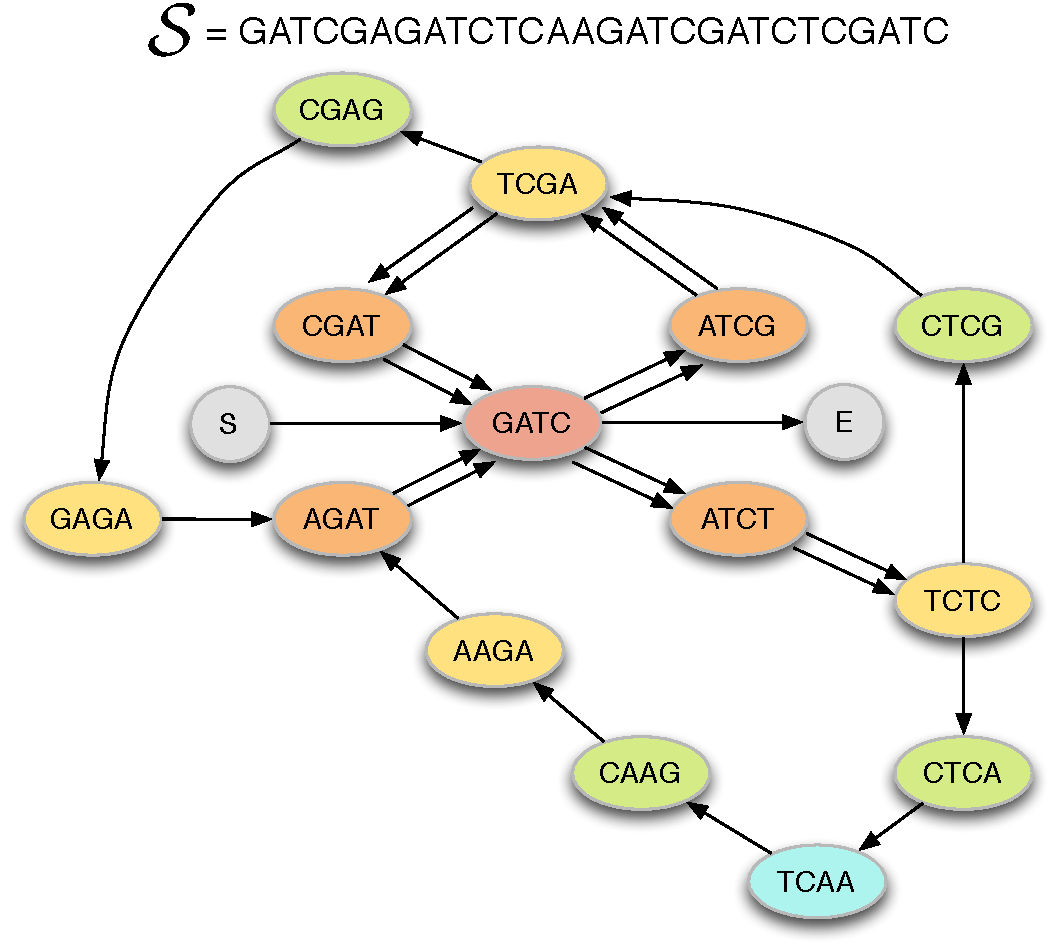
\includegraphics[width=0.7\linewidth]{figures/huffmer_node_neighborhoods}
    \caption{\textbf{De Bruijn graph with multi-edges allows one to build dictionaries that preferentially select high-frequency substrings.} The greedy algorithm would select \texttt{GATC} node due to its high degree and will update edge weights in its neighborhoods up to $k-1$ edges away.}
    \label{fig:denovo:debruijn}
  \end{figure}

  To construct such a dictionary, we need an algorithm that would allow us to select non-overlapping high-frequency kmers. De Bruijn graph over $\seq$ explicitly encodes overlaps between consecutive kmers. We enhance the graph with edge weights where $e(u,v)$ has a weight $w$ if kmer $d_u$'s $(k-1)$ long suffix is $d_v$'s $(k-1)$ long prefix, and a subsequence $d_u + d_v[k]$ (or, equivalently, $d_u[1] + d_v$) was observed in $\seq$ $w$ times (see Figure~\ref{fig:denovo:debruijn}). Given such graph $G_k(\seq)$, the weighted in-degree of a vertex $indeg(u)$ is equivalent to the number of times kmer $d_u$ appeared in $\seq$. Node $u$'s immediate neighborhood $N_1(u)$ represents all nodes $v_1, v_2, \ldots$ such that $d_u$ overlaps with any of the $d_v$ kmers by $(k-1)$ nucleotides. Similarly, nodes in the neighborhoods $N_2, N_3, \ldots, N_{k-1}$ represent kmers that share $(k-2), (k-3), \ldots, 1$ nucleotides with $d_u$. Selecting $d_u$ to be in $D$ implies that no kmer instances that overlap with any of the copies of $d_u$ in $\seq$ can be added to $D$. To reflect this fact, we have to progressively prune edges in neighborhoods $N_1(u), N_2(u), \ldots, N_{k-1}(u)$ thus decreasing the in- and out-degrees of the vertices in $N_1(u), N_2(u), \ldots, N_{k-1}(u)$. 

  % XXX Russell -- can you transform it to set cover and use a set cover solver?

  We believe that in general this problem is similar to set cover~\cite{SetCoverIsHard} with individual kmers being the items and their neighborhoods $N_1, \ldots, N_{k-1}$ forming the set of sets of which we seek the minimum subset covering all of the items. However, this problem is different from set cover in that kmer multiplicities and overlaps have to be modeled explicitly. The complexity of the algorithm remains an unsolved question; in the meantime, we propose a greedy algorithm to build a dictionary $D$ from the de Bruijn graph $G_k(\seq)$:
  
  \begin{algorithm}[H]
   \KwData{Sequence $\seq$, $k$ -- kmer length}
   \KwResult{$D$ -- a dicitonary of frequent kmers that cover $\seq$ }
   build de Bruijn graph $G(\seq)$\;
   pick $u$ -- highest degree vertex, add $d_u$ to $D$\;
   \While{$\textrm{deg}(u) > 1$}{
    \For{$i \leftarrow 1$ \KwTo $k-1$}{
      \For{$v  \in N_i(u)$}{
        remove edge
      }
    }
    pick $u$ -- highest degree vertex\;
   }
   \While{$\textrm{deg}(u) > 1$}{
    collapse path $\mathcal{P} \ni u$ to $d_{\mathcal{P}}$\;
    add $d_{\mathcal{P}}$ to $D$\;
   }
   \caption{Greedy kmer selection}
   \label{algo:greedy}
  \end{algorithm}
  %

  

  Unlike the dictionary built to cover the whole input string $\seq$, building a dictionary by preferentially selecting high-frequency kmers does not guarantee that words in $D$ will cover $\seq$. In the worst case, kmers could be selected in a way that any two kmers are separated by $(k-1)$ uncovered nucleotides (\ie~``holes'') resulting in less that $|\seq| / 2$ being covered. It is feasible that such adversarial string could be constructed, however, given that DNA sequence has a limited alphabet and its kmer distribution is highly skewed, we expect the words from a kmer dictionary to cover most of the string. Our tests using Algorithm~\ref{algo:greedy} show that kmers in the dictionary will usually cover over $80\%$ of $\seq$.

  %%%%%%%%%%%%%%%%%%%%%%%%%%%%%%%%%%%%%%%%%%%%%%%%%%%%%%%%
  % 
  %%%%%%%%%%%%%%%%%%%%%%%%%%%%%%%%%%%%%%%%%%%%%%%%%%%%%%%%
  \subsection{Building a dictionary with kmers of mixed lengths}

  Instead of allowing some subsequences in $\seq$ to remain uncovered, we can vary the word length and require that $d_i$s cover the all of $\seq$. We will call a decomposition of $\seq$ into separate words $d_i$ a \textit{parse} $P$ and will require that:
  %
  \begin{align}
  \label{eqn:constraints}
  \sum_{d_i \in D} f_i |d_i| = |\seq|~\textrm{and}~P(\seq, D) = \seq,
  \end{align}
  %
  in other words, we require that we can recover the original sequence $\seq$ using the parse $P$ and we use no more $d_i$s than are necessary.
  Due to these constraints, a common approach of counting kmers using a sliding window of length $k$ over the sequence $\seq$ will always result in a dictionary $D$ such that $\sum_{i} f_i |d_i| \geq |\seq|$ and worse compression ratios (data not shown).

  The following example demonstrates the benefits of allowing for variable length word in the shared dictionary data structure:
  %
  \begin{align*}
    \seq &= \textrm{\underline{GATC}GA\underline{GATC}TCAA\underline{GATC}\underline{GATC}TC\underline{GATC}} \\
    % D_2 &= \{ GA: 6, TC: 7, AA: 1 \} \\
    % D_4 &= \{ GATC: 2, GAGA: 1, TCTC: 2, AAGA: 1, TCGA: 1\} \\
    D_{2,4} &= \{GATC: 5, GA: 1, TCAA: 1, TC: 1\}
  \end{align*}
  %
  Encoding the string using a dictionary $D_2$ of non-overlapping 2-mers results in $\compseq = 0010000111010010011001$ 21 bits long. If we consider a set of non-overlapping 4-mers $D_4$, we 
  % obtain Huffman codes $\{ GATC=00, GAGA=10, TCTC=01, AAGA=111, TCGA=110\}$ resulting in a 
  can compress the string down to 16 bits. However, \texttt{GATC} occurs 5 times within the string. By selecting \texttt{GATC} as one of the 4-mers and adding \texttt{TCAA}, \texttt{GA} and \texttt{TC} to the dictionary $D_{2,4}$, we are able to compress $\seq$ down to 13 bits while satisfying the covering constraint. 
  % This example shows that there are instances when mixing kmers of different lengths and selecting kmers at positions other than those that align with the $k$-induced boundaries may result in a better compression.

  To ensure that kmers of various lengths are selected into $D$, we maintain several de Bruijn graphs $G_{k-1}(\seq), G_{k-2}(\seq), \ldots$ and prune them in a manner consistent with pruning in $G_{k}(\seq)$. Shorter kmers occur at higher frequencies than longer kmers and kmer frequencies need to be normalized across different kmer lengths to account for differences in their distributions. At each step, we compute the mean kmer frequency $\mu_j$ over kmers currently in $G_{j}$ and normalize kmer counts in $G_j$ to be $f_i / \mu_j$. We select a single kmer $d^*$ with the highest normalized frequency over all kmers within a given $G_j$ and over all kmer lengths: $d^* = \max_j \max_i f_i / \mu_j$ where $i$ varies over all kmers of length $j$. We update the means $\mu_j$ at every iteration to be able to greedily select the most frequent kmers among the remaining kmers.

  To quickly select the most frequent kmer, we maintain a priority heap $H_j$over kmers and their frequencies for every kmer length $j$. When a kmer in one of the graphs $G_{j}(\seq)$ is selected, we remove it from the top of the corresponding heap $H_j$, update all relevant neighborhoods in $G_{j}(\seq)$ and frequencies in $H_j$ for kmers that overlapped $d^*$. Then for every $G_l$ for $l > j$ we visit all $l$-mers that contain the chosen $j$-mer and update their frequencies. Analogously, we visit graphs $G_l$ where $l < i$ and visit nodes representing $l$-long prefixes and suffixes of $d^*$ and decrease their counts accordingly.


  %%%%%%%%%%%%%%%%%%%%%%%%%%%%%%%%%%%%%%%%%%%%%%%%%%%%%%%%
  % 
  %%%%%%%%%%%%%%%%%%%%%%%%%%%%%%%%%%%%%%%%%%%%%%%%%%%%%%%%
  \subsection{Building a shared dictionary across multiple datasets}

  We extend the problem of learning a dictionary given a single input string $\seq$ to learning a dictionary given multiple related strings $\seq_1$, $\seq_2$, \ldots. There are several ways to approach this task: concatenating strings $\seq_1$, $\seq_2$, \ldots into a single string reduces the problem to its original formulation. Another alternative is to learn dictionaries $D_1$, $D_2$, \ldots independently and then merge them into a single large dictionary $D$. When all dictionaries use uniform kmer legnth $k$, merging individual dictionaries is as straightforward as building a union of kmers. 

  When counting kmers, the frequency distribution is long-tailed and contains many kmers occurring in the dataset only once. These kmers could be a result of natural variation in sequence, or a result of sequencing errors.  These kmers may inflate the size of the final dictionary while providing little to no gain in compression. When building kmer dictionaries, we consider several frequency cutoffs for which we remove all kmers below that frequency.

    % -- strategies for building a dictionary across datasets (kmer union, kmer intersection)

  % XXX exclude kmers w/ low counts -- too many of them and they are most likely the sequence errors

  % XXX more detail here

%%%%%%%%%%%%%%%%%%%%%%%%%%%%%%%%%%%%%%%%%%%%%%%%%%%%%%%%
\section{Optimal string parsing given a dictionary with codes}

  % additional definitions
  \newcommand{\esc}{\texttt{ESC}\xspace}
  \newcommand{\escremap}{\texttt{ESCR}\xspace}


  There are two challenges to using a dictionary $D$ created by the above scheme when compressing a new string $\seq$. First, there may be many parses of $\seq$ into substrings from $D$ some of which are better than others, and, second, $\seq$ may contain substrings that cannot be covered by $D$. We propose a dynamic programming approach to solv the problem of multiple possible parses and suggest two ways of handling novel substrings of $\seq$.

  More specifically, to handle parts of $\seq$ not covered by $D$ (so-called ``holes''), we insert an special escape symbol $\esc$ symbol into $D$ and assign it relatively high frequency $f_{\esc}$ that we estimate from the experimental data. To encode a substring $h \in \seq$ that can not be covered by $D$, we write out a Huffman code for $\esc$, followed by the length of $h$, followed by the two-bit encoding of $h$. Using $\esc$ code allows to unambigously differentiate a two-bit encoded substring from a Huffman code for a substring in $D$.

  When a substring $h$ has a string $d_i \in D$ such that Hamming distance between $h$ and $d_i$ is one (a substitution), it may be beneficial to use the Huffman code for $d_i$ in combination with a short edit script to encode $h$. To distinguish between two-bit encoded substrings and substrings with edit scripts, we introduce a second escape symbol $\escremap$. When encoding $h$, we write out a binary code for $\escremap$, followed by the $c_i = D[d_i]$, followed by $\lceil \log_2 k \rceil$ bits describing the position $1 \leq p \leq k$ of the substitution, followed by two bits encoding the character in $h$ in position $p$.

  % ***(C) It's unclear if this is a good way to do this; the other option is to always include ‘A’ ‘C’ ‘G’ and ’T’ in D.***

  We use a dynamic programming approach to find a parse of $\seq$ where most of the string is covered by $D$. More formally, given a string $\seq$, we seek an encoding $\compseq$ of the original string with codes from $D$ such that the length of encoding is minimized. For such substrings of $\seq$ that can not be covered with any $d_i$, we assign a penalty, $d_{\mathrm{esc}}$ and encode this gap with two bit encoding. For each character $i$ of $\seq$, we decide whether it is more beneficial to replace the last $k$ characters with a code from $D$, i.e. use an existing code for $h = \seq[i-k,i]$ kmer (handled by $\mathrm{OPT_{kmer}}$ case), or to incur the penalty for two-bit encoding the substring. If there is no code for $h$ in the dictionary, we choose to start a new hole or extend a previously opened hole (handled by $\mathrm{OPT_{hole}}$ case):
  %
  \begin{align}
  \mathrm{OPT_{kmer}}(i) & = \left \{
      \begin{array}{l l}
        %first choice
        + \infty \\
        % second choice
        |D(h)| + \mathrm{OPT_{kmer}}(i-k-1) \\
        |D(h)| + \mathrm{OPT_{hole}}(i-k-1) \\
      \end{array} \right. \\
  %
  \mathrm{OPT_{hole}}(i) & = \left \{
      \begin{array}{l l}
        %first choice
        |\esc| + |\mathrm{pos}| + 2 + \mathrm{OPT_{kmer}}(i-1) \\
        % second choice
        2 + \mathrm{OPT_{hole}}(i-1) \\
      \end{array} \right.
    \label{eqn:denovo:twobit}
  \end{align}
  %

  When we use a remapping strategy for encoding parts of $\seq$ not covered by $D$, we modify the dynamic programming formulation for $\mathrm{OPT_{kmer}}$ only slightly:
  %
  \begin{align}
  \mathrm{OPT_{kmer}}(i) & = \left \{
      \begin{array}{l l}
        %first choice
        + \infty \\
        % second choice
        |D(h)| + \mathrm{OPT_{kmer}}(i-k-1) \\
        |D(h)| + \mathrm{OPT_{hole}}(i-k-1) \\
        |\escremap| + |D(h^*)| + \lceil \log_2 k \rceil + 2~+ \mathrm{OPT_{kmer}(i-k-1)} \\
        |\escremap| + |D(h^*)| + \lceil \log_2 k \rceil + 2~+ \mathrm{OPT_{hole}(i-k-1)} \\
        \label{eqn:denovo:remap}
      \end{array} \right. \\
  \end{align}
  %
  Two new cases in the $\mathrm{OPT_{kmer}}(i)$ handle the alternative of remapping the observed subsequence $h$ onto a known kmer $h^*$ that is already in $D$. First, we search $D$ for a kmer $h^*$ that is within distance 1 of $h$. If such kmer is found, then we spell out the binary escape code $\escremap$ indicating that the kmer was remapped, followed by the binary code for the matching kmer $D(h^*)$, followed by an encoding of the difference(s) between $h$ and $h^*$. We allow for a single mismatch between $h$ and $h^*$ in the Equation~\ref{eqn:denovo:remap}, which we can encode by spending $\lceil \log_2 k \rceil$ bits to encode the mismatch's position within $h^*$ and additional 2 bits to encode what the letter in $h^*$ should be replaced with when decoding the compressed stream.

  % remapping
  To efficiently find $h^* \in D$ that is only a Hamming distance one away from $h$, we explore all possible kmers that have only a single mismatch with $h$. To do so, we iterate through every nucleotide in $h$ and test if $D$ contains a kmer with either of the 3 alternative bases in that position. For a kmer of length $k$, that amounts to going through and validating $3k$ kmers. Among the remapped kmers that are present in $D$, we pick the one with the shortest binary code. Generating these $3k$ kmers is much faster than going through every kmer in $D$ and computing the Hamming distance between $h$ and every $d_i$ and we are able to perform the remapping without a significant increasing the running time. Similar thinking can be extended to handling more mismatched between $h$ and $h^*$, however, in practice, we  observe that increasing the number of allowed mismatches does not improve $\seq$ coverage or compression ratio in a significant way.

  The proposed dynamic programs run in the time linear to the length of the input string $\seq$. Indeed, at every step $i$ we only need to evaluate a constant number of choices (3, 2, or 5 --- see Equations~\ref{eqn:denovo:twobit} -- \ref{eqn:denovo:remap}) each of which takes constant time. At the same time, we will have to maintain two arrays to store the values for $\mathrm{OPT_{kmer}}(i)$ and $\mathrm{OPT_{hole}}(i)$. However, further analysis shows that we only ever consider a single previous solution to either of the optimal values, so instead of maintaining two arrays of size $|\seq|$, we can simply maintain two variables holding the optimal values for at the previous step for $\mathrm{OPT_{kmer}}(i)$ and $\mathrm{OPT_{hole}}(i)$ respectively. This results in $O(|\seq|)$ runtime algorithm with $O(1)$ memory requirements.

%%%%%%%%%%%%%%%%%%%%%%%%%%%%%%%%%%%%%%%%%%%%%%%%%%%%%%%%
%
%%%%%%%%%%%%%%%%%%%%%%%%%%%%%%%%%%%%%%%%%%%%%%%%%%%%%%%%
\section{Compressing the dictionary for transmission}

To encode the dictionary, we only need to efficiently encode kmers and frequencies associated with them, and the Huffmer codes can be restored unambiguosly on the receiver's side. A straighforward way of encoding the kmers is to write out their two-bit representations along with frequencies. However, a bit tree~\cite{PathEncode} is a more efficient way of encoding strings of the same length. Bit tree performs significantly better than general-purpose compression tools when used on kmer sequences and is orders of magnitude better than the commonly used 2-bit encoding (Table~\ref{fig:denovo:bittree}). Bit tree achieves compression ratios as low as 0.09 bits per kmer ($k=10$). Unlike bloom filters which are used commonly to hold sets of kmers, the bit tree can reconstruct the original kmer set.

To compare bit tree to common-purpose compressors, we counted canonical kmers at different lengths $k = 10, \ldots, 24$ on a human RNA-seq sample (SRA run ID \texttt{SRR037452}), and then compressed kmer sequences using \texttt{plzip} (Table~\ref{fig:denovo:bittree}). We then used bit tree on the same set of kmer sequences. Additionally, we compared results to a bit tree post-compressed with \texttt{plzip} --- when many kmers share a common prefix, the tree binary representation would be highly self-similar and may benefit from downstream compression. Indeed, for dense kmers sets at $k=10$ and $k=12$ that contained $50\%$ and $48\%$ of the total possible number of kmers ($4^k$), post-processing step improved the compression ratio from $36.6$ and $42.7$ to $949.0$ and $373.6$ respectively.

\begin{table}[ht]
  \centering
  \begin{tabular}{c r r r r}
  \toprule
  k & kmer count & *.lz & bit tree & bit tree + lz \\
  \midrule
  10 &   877,527 & 1,267,692 & 157,377 & 6,083 \\
  12 & 3,257,484 & 16,768,251 &  2,497,689 & 285,137 \\
  14 & 4,134,104 & 209,338,609 & 27,138,873 &  20,177,568 \\
  16 & 4,302,693 & 460,208,443 & 102,499,425 & 86,198,199 \\
  18 & 4,380,861 & 549,068,270 & 195,150,889 & 158,596,795 \\
  20 & 4,444,210 & 578,979,167 & 277,692,945 & 217,172,798 \\
  22 & 4,500,972 & 583,681,685 & 342,331,145 & 258,201,259 \\
  24 & 4,552,444 & 566,885,773 & 385,700,657 & 282,575,128 \\
  \bottomrule
  \end{tabular}
  \caption{ \textbf{Bit tree outperforms plzip on sets of kmer sequences.} Bit tree  can achieve over 900x reduction in size when encoding dense kmers sets ($k=10,12$). Sizes show in bytes. Canonical kmers were counted using Jellyfish~\cite{Jellyfish}.}
  \label{fig:denovo:bittree}
\end{table}

Bit tree stores the input sequences in their alphabetic order, so the associated frequencies have to be reordered to match kmer order when sending the dictionary over the network. Encoding the kmers and the frequencies separately improves homogeneity within these two sets and results in better dictionary compression rates.

%%%%%%%%%%%%%%%%%%%%%%%%%%%%%%%%%%%%%%%%%%%%%%%%%%%%%%%%
\section{Results}

  \subsection{Remapping kmers preferable in optimal string encoding}

  Earlier, we proposed two alternative strategies of addressing subsequences not covered by the coding dictionary $D$: to encoded the uncovered sequence using a 2-bit encoding and, alternatively, first attempt to find a kmer in $D$ that is Hamming distance 1 away from the subsequence in question. To test these two strategies, we learned a dictionary on each of the test files and then tested dictionary's performance on every file (see Table~\ref{table:denovo:twobitvsremap}). Testing for the presence of similar kmers allows to improve compression ratio in the case of self-encoding as well as in the case of the dictionary training file and the target file containing sequence from different species and type of experiment.

  \begin{table}
  	\centering
  	\subfigure[2-bit encoding]{
        \label{subfig:twobitenc}
        % \caption{k=20, kmer counting: nonoverlapping, twobit encoding for holes}
		\begin{tabular}{c r r r}
		 \toprule
		\backslashbox{target}{dictionary} & A & B & C \\ 
		\midrule
		A & 0.10 & 0.38 & 0.37 \\
		B & 0.41 & 0.12 & 0.41 \\
		C & 0.42 & 0.42 & 0.12 \\
		\end{tabular}
    }
    \subfigure[Remapping + 2-bit]{
    	\label{subfig:remappingenc}
        % \caption{k=20, kmer counting: nonoverlapping, remap + twobit encoding for holes}
		\begin{tabular}{c r r r}
		 \toprule
		\backslashbox{target}{dictionary} & A & B & C \\ 
		\midrule
		A & 0.09 & 0.25 & 0.24 \\
		B & 0.25 & 0.10 & 0.25 \\
		C & 0.26 & 0.26 & 0.10 \\
		\end{tabular}
    }
	\caption{\textbf{Remapping strategy for encoding uncovered sequence significantly outperforms the two-bit encoding approach.} Each column represents a file on which the dictionary $D$ was trained, while rows represent files which were compressed. Each cell reports a compression ratio (compressed size over original sequence size). Dictionaries were learned for $k = 25$ and under the constraint of complete $\seq$ coverage. Datasets used for these computations: A --- \texttt{SRR519063}, B --- \texttt{SRR635193}, C --- \texttt{ERR233214}.}
	\label{table:denovo:twobitvsremap}
  \end{table}

  %%%%%%%%%%%%%%%%%%%%%%%%%%%%%%%%%%%%%%%%%%%%%%%%%%%%%%%%
  \subsection{Performance when building the dictionary and encoding on the same dataset}

  We achieve compression rates competitive with state of the art tools~\cite{Sahinalp2012,Jones2012} when the dictionary $D$ is built on the same dataset that was use to construct $D$ under the constraint of completely covering the input string $\seq$ (Figure~\ref{fig:denovocompr:varyK}). Here, the input string $\seq$ was constructed by ordering and concatenating reads appearing in the FASTA file. Compression performance improves steadily as we increase the kmer length $k$. However, as we increase $k$, the number of kmers in the dictionary and its size also grows (data not shown). The dictionary learned on a single file and applied to a different input string $\seq$ results in decreased performance (see Table~\ref{subfig:remappingenc}).

  % Optimizing the dictionary for coverage produces better compressed files when compared to using a dictionary that sacrificed coverage for the kmer frequency (XXX show data).
  
  
  %%%%%%%%%%%%%%%%%%%%%%%%%%%%%%%%%%%%%%%%%%%%%%%%%%%%%%%%
  \subsection{Building the dictionary and compressing across related datasets}

  	% XXX dictionary size on the single cell RNA-seq
  	%   -- dicitonary size keeps growing

    To test the general applicability of the shared dictionary scheme, we learned the dictionary on a large collection of related data. For this task, we have selected a set of single cell RNA-seq experiments on human embryonic cells done by a single laboratory (SRA study ID: \texttt{SRP011546}). We learned kmer dictionaries one dataset at a time and progressively built a union dictionary. We excluded kmers with frequency $f_i < 2$ from the dictionary to slow down the dictionary size growth. For every new kmer $d_i$ being added to the dictionary, we first attempted to find a kmer $d_j$ already in $D$ that was within Hamming distance 1 away from $d_i$. We would only add $d_i$ to the dictionary if there were no $d_j$ found to further limit dictionary growth. However, the size of the kmer union increased as we added more datasets  without an indication that it was leveling off (Figure~\ref{fig:denovo:rnaseq}). We observed the same trend when only considering kmers of frequency $f_i \ge 10$ and $f_i \ge 100$. These facts led us to believe that the shared dictionary learned on a collection of related datasets would necessarily be large to remain competitive with other state of the art compression approaches.

    \begin{sidewaysfigure}[ht!]
    % \begin{figure}
    	\centering
      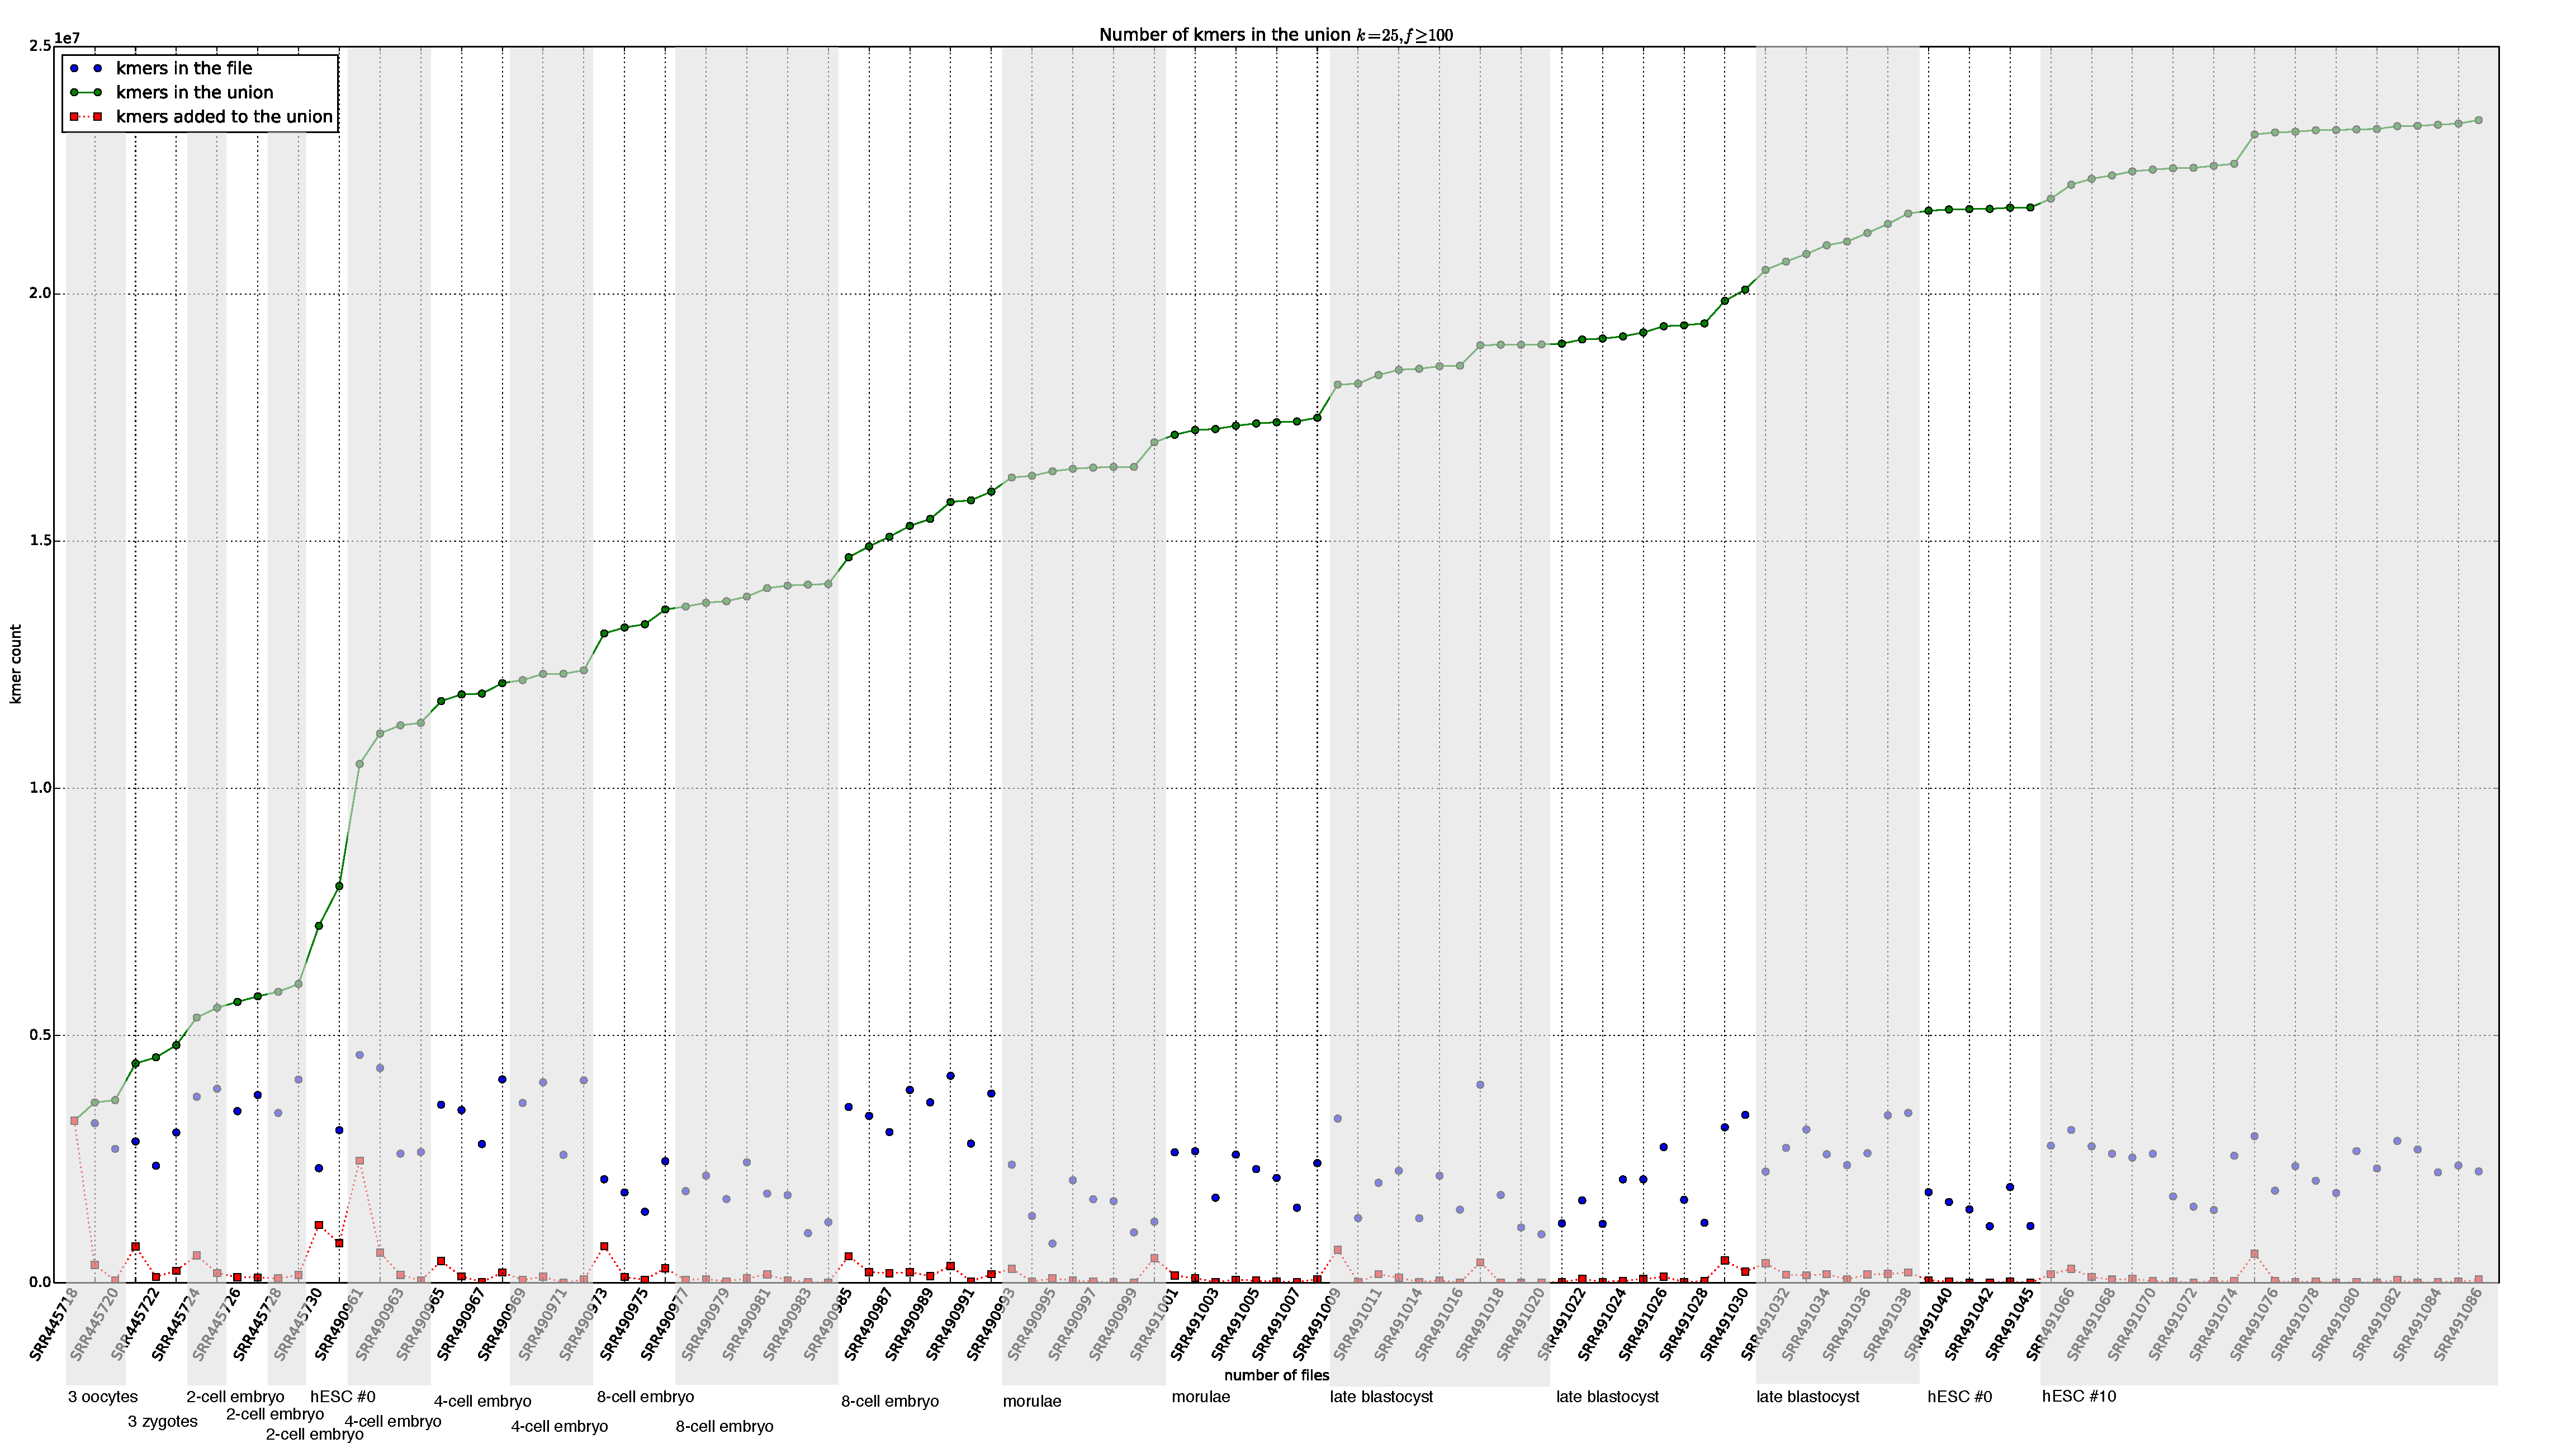
\includegraphics[width=\linewidth]{figures/huffmer-rnaseq-experiment-cells}
      % 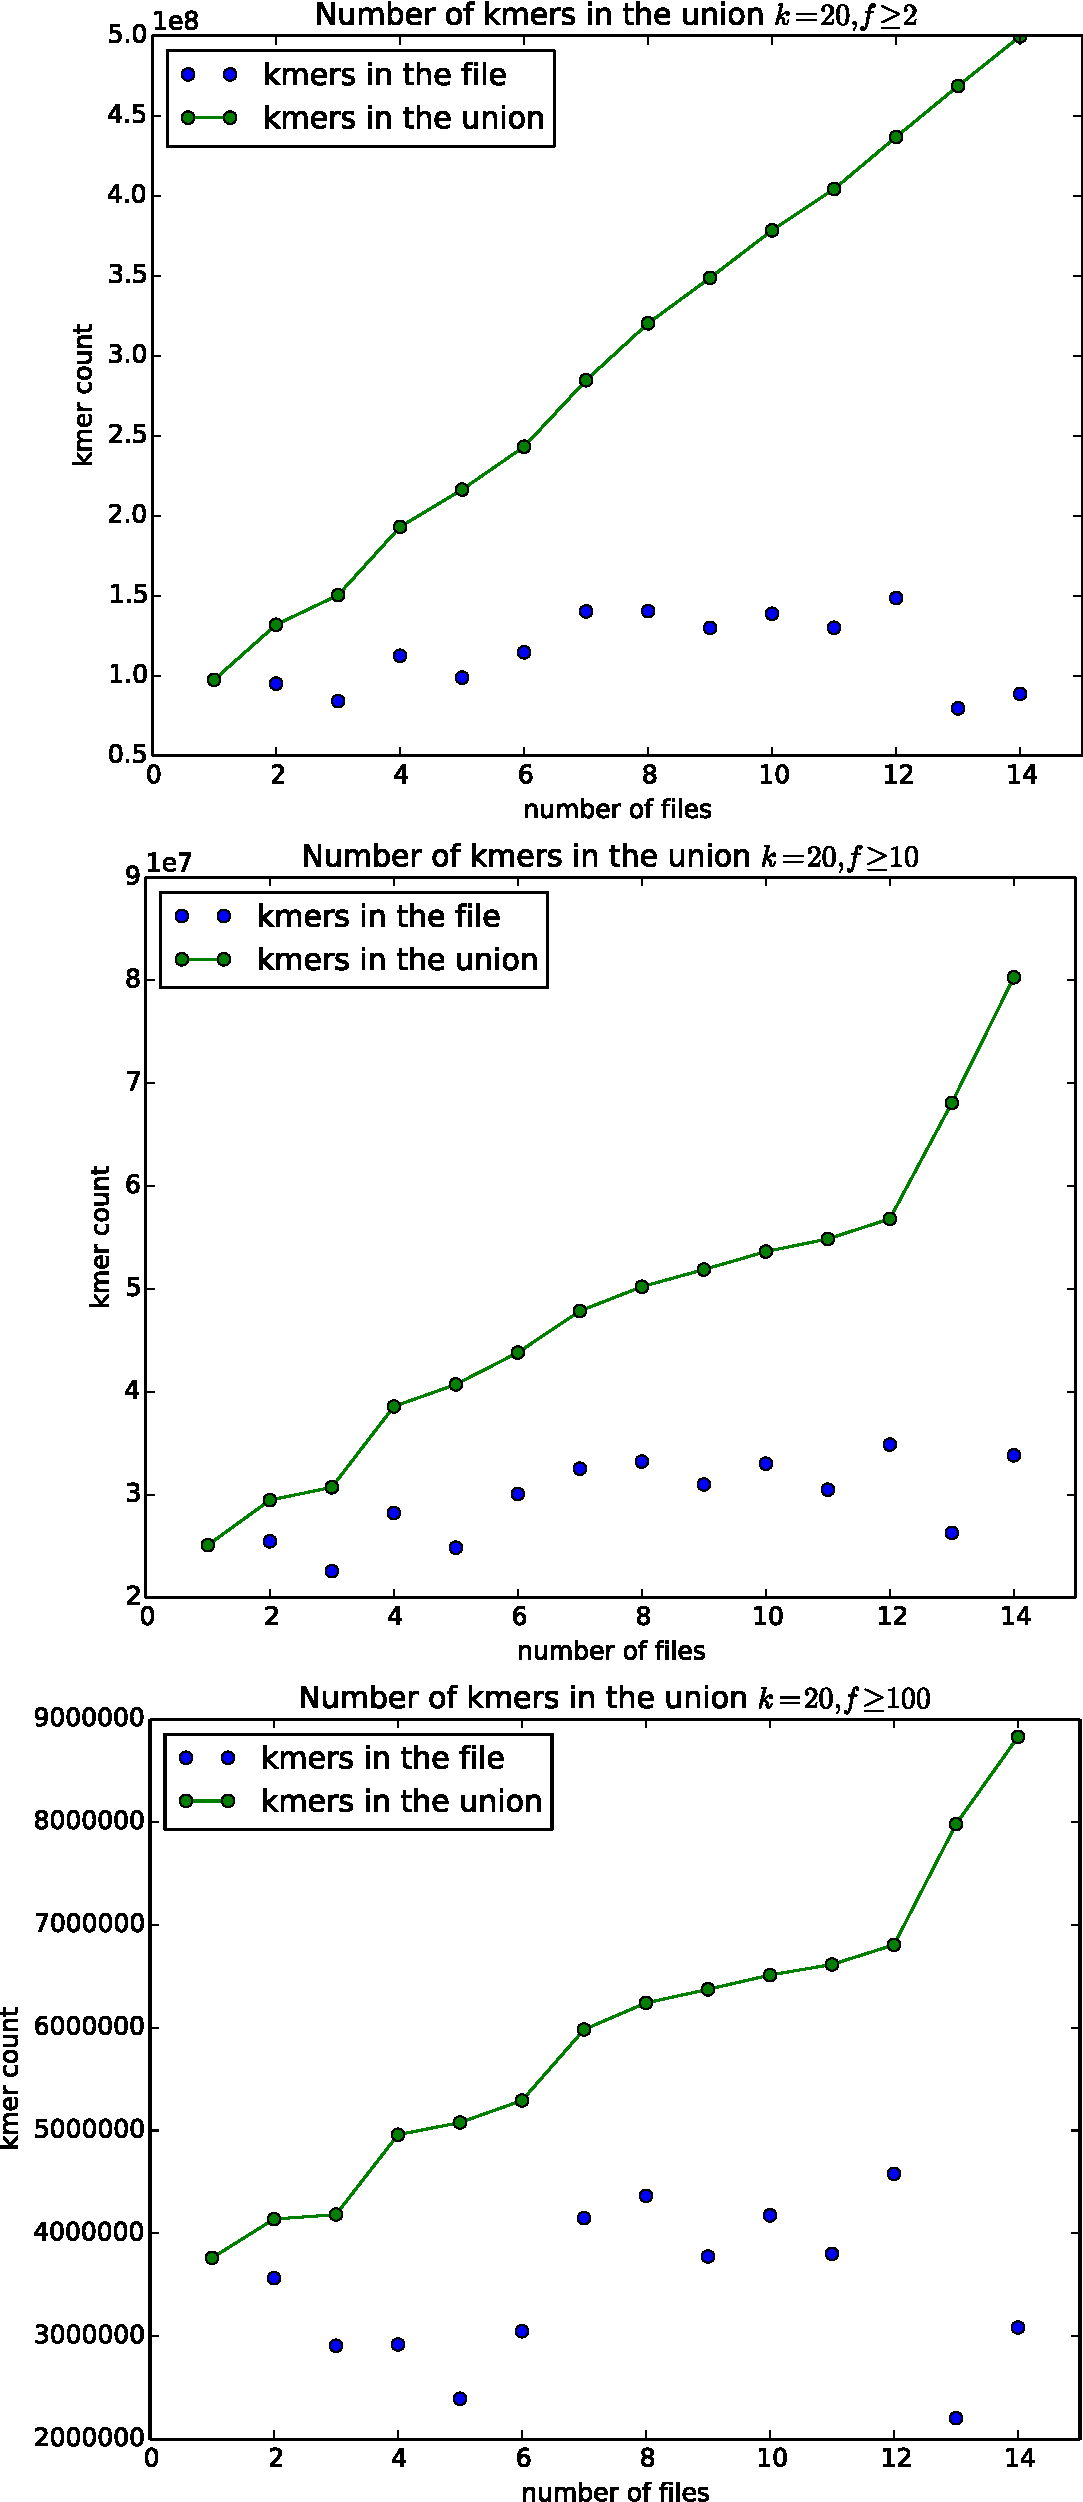
\includegraphics[width=0.6\linewidth]{figures/rnaseq-kmer-union-k=20-combined}
      \caption{\textbf{Dictionary size increases with new data being added to the dicitonary union.} We plot the number of kmers in the union dictionary as new RNA-seq data is being added. Data shown is derived from an experiment with SRA ID \texttt{SRP011546}.}
      \label{fig:denovo:rnaseq}
    \end{sidewaysfigure}
    % \end{figure}

    To investigate the source of the kmer diversity in single cell RNA-seq data, we examined the overlap between kmers found in the human transcriptome and kmers in the individual RNA-seq files (Table~\ref{tab:denovo:transciptome_overlap}). We selected a single representative file from the embryonic cell experiment and added new human RNA-seq data generated by different labs and derived from different tissues. Surprisingly, we found that for a range of read lengths and sequencing depths, the number of kmers shared between the dataset and the transcriptome was highly variable and does not exceed 30\% of all kmers in $T$. For example, kmers from a human RNA-seq experiment on placenta sample contained only 2M kmers that were also found in the transcriptome and 246M kmers not found in $T$. Higher read counts and longer read lengths were correlated with larger intersections between the set of kmers $D$ and kmers in transcriptome $T$ (except for the placenta sample). The source of such significant divergence between kmer sets in $D$ and $T$ could be explain by the sequencing errors and natural variation between human samples within the sequencing experiment.
    
    %   -- most kmers are not even in the transcriptome
    \begin{table}
      \centering
      \begin{tabular}{l c r r r r r}
          \toprule
          File  & Cell type & Read count & $|r|$ & $D \cap T$ & $D \backslash T$ & $T \backslash D$ \\
          \midrule
          SRR037452 & RNA-seq, brain & 13552276 & 35 & 18513744 & 59214972 & 94883622 \\
          SRR1294122  & RNA-seq, CD34+ & 39666314 & 101 & 58694264 & 408807236 & 54703102 \\
          SRR034940 & WGS & 72795628 & 100 & 28697479 & 916749539 & 84699887 \\
          SRR553463 & RNA-seq, neutrophil & 49771919 & 49 & 34291992 & 118624324 & 79105374 \\
          SRR553460 & RNA-seq, neutrophil & 66552453 & 49 & 35242903 & 119608311 & 78154463 \\
          SRR527697 & RNA-seq, placenta & 169606661 & 101 & 2053392 & 246196849 & 111343974 \\
          SRR445718 & RNA-seq, oocyte & 32943665& 101 & 32051874 & 246196849 & 81345492 \\
          \bottomrule
      \end{tabular}
      \caption{\textbf{Number of kmers shared between human RNA-seq experiments and annotated human transcriptome.} Here, $D$ is the set of kmers counted on the corresponding dataset, $T$ -- kmers from the transcriptome. The transcriptome had a total of 115M kmers.}
      \label{tab:denovo:transciptome_overlap}
    \end{table}

    Finally, we tested the similarity between the kmer sets in the RNA-seq data. For that, we constructed a small matrix of shared kmer counts across five datasets (Table~\ref{tab:denovo:kmer_overlap}). We observe that across five human RNA-seq datasets, the kmer set similarity is very low with highest Jaccard similarity at 0.27. Our intuition was that sequencing error rate contributed to both the number of unique kmers not shared with the transcriptome and to the dissimilarity across seemingly related data. 

    %   -- XXX but the reads do align well to the genome

    To evaluate the quality of RNA-seq data, we used STAR~\cite{DobinSTAR} to align RNA-seq reads from \texttt{SRR037452} and \texttt{SRR1294122} to human transcriptome while limiting alignments to have at most two edits. A large percent of reads aligned in both cases indicating that a large subset of reads was of acceptable quality (65\% and 80\% of reads aligned correspondingly).

    %   -- kmer set overlaps between the sets is small
    \begin{table}
      \centering
      \begin{tabular}{l c c c c c}
          \toprule
          & SRR037452 & SRR1294122 & SRR527697 & SRR553460 & SRR553463 \\
          \midrule
          SRR037452 & 1.000 & 0.040 & 0.003 & 0.061 & 0.058 \\
          SRR1294122 & 0.040 & 1.000 & 0.005 & 0.077 & 0.075 \\
          SRR527697 & 0.003 & 0.005 & 1.000 & 0.005 & 0.005  \\
          SRR553460 & 0.061 & 0.077 & 0.005 & 1.000 & 0.270  \\
          SRR553463 & 0.058 & 0.075 & 0.005 & 0.270 & 1.000 \\
          \bottomrule
      \end{tabular}
      \caption{\textbf{Jaccard similarity between pairs of kmer sets.} Jaccard similarity $J = |D_1 \cap D_2 |/ |D_1 \cup D_2| $ between kmer sets in human RNA-seq datasets did not exceed 0.27.}
      \label{tab:denovo:kmer_overlap}
    \end{table} 

    We conclude that the dictionary size required for our compression scheme to be competitive with other de novo methods would be too large to justify transmitting it even once (for example, to use to to decompress the 100 single cell RNA-seq files). At the same time, high mapping rate suggests that a reference-based approach might be more promising given an efficient way to encode the differences between the aligned reads and a reference sequence.

  %   -- CONCLUSION: too much variability, a single error , plus read boundaries matter


%%%%%%%%%%%%%%%%%%%%%%%%%%%%%%%%%%%%%%%%%%%%%%%%%%%%%%%%%%%%%%%%%%%%%%%%%%%%%%%
%
%%%%%%%%%%%%%%%%%%%%%%%%%%%%%%%%%%%%%%%%%%%%%%%%%%%%%%%%%%%%%%%%%%%%%%%%%%%%%%%
\section{Discussion and conclusions}

  Using kmer collections as shared information across datasets offers a novel  solution to the sequence compression challenge and breaks the middle ground between \textit{de novo} and reference-based compression techniques. It is competitive with the state of the art tools under certain conditions, but provides only marginal benefits when applied in a more general setting.

  We considered different regimes for building a set of frequently occurring substrings within an input string $\seq$. We developed efficient algorithms for learning such dictionaries while maximizing $\seq$'s coverage and selecting the most frequent substrings into $D$. We develop an optimal algorithm with linear runtime that, given a dictionary $D$, will find an optimal parse in the string $S$ minimizing its compressed size.

  % not leverage the repetitive nature of the sequence enough to provide a significant advance.

  % The problems of building the most efficient dictionary that both covers most of the reference sequence while capturing most frequent substrings is of general interest: XXX is it?
  
  % - we developed a framework for building shared dict and optimally encoding strings with it

% - defined different objectives for shared inform dictionaries

% - defined an optimal parse of a string given a dictionary that take O(n) to run

% - performed tests showing that despite sequence aligning well to the transcript one, kmer sets are too different

% - requiring the presence of the same exact kmers is too strict. dictionary coders like SCALCE and MINCE get an edge by replacing whole swathes of sequence

% -- kmer dictionary will always spend bits when seeing the same kmer again and again, other dictionaries will use this to their advantage

% -in addition, Huffman approach will always code according to the frequencies in the training data, but test data could be highly scewed

	We test our dictionary construction algorithms on a collection of related RNA-seq datasets and show that due to variation in data, the size of the dictionary needed to provide competitive compression rates would be too large to be practical. However, RNA-seq data's high mapping rates suggest that human transcriptome or genome could serve as shared information given that we can encode the differences between the reads and the reference sequence efficiently.

% -- error rates and read boundaries do no allow for efficient shared dictionary construction based on kmers


  \subsubsection{Computing on compressed data}

  % \todo assume Huffman encoding

  The Huffman-based dictionaries can be extended in a way that would allow for computing on the compressed streams. To allow partial decompression, $\compseq$ can be enhanced by storing several pointers into the compressed stream that align with kmer boundaries. The shared dictionary itself can be used as a search index: given a search subsequence $s$, we can query $D_k$ for all $k$-long kmers in $s$ to be able to tell if $s$ may occur in $\seq$. If $D$ contains at least some kmers from $s$, we would perform a direct search in $\compseq$ for a bit subsequence $c(s_k)$ where $s_k$ is the matched kmer that aligns with the kmer boundaries.

  \subsubsection{Using grammar as shared information for de novo sequence compression}

  Sequences of nucleotides are in no way a random sequence of four characters. Huffman coding exploits this fact by assigning frequently appearing kmers shorter codes. However, it is conceivable that higher-order organization exists within the sequence, akin to a language grammar. Our initial experiments with Sequitur~\cite{Sequitur}, a compression algorithm based on inferring grammars in text, show that a grammar-based approach is competitive with specialized sequence compression tools like SCALCE~\cite{Sahinalp2012}. Changes to Sequitur's algorithm, such as only considering subsequences of a given minimum length $k$, may further improve its performance. However, sequencing errors have to be explicitly taken into account since they will not adhere to the grammar learned on a reference genome or a different set of reads. Additionally, a grammar learned on one set of reads (or on a reference genome) would have to be able to handle the fact that read boudaries may be different in another read set and the rules learned originally may cross these boundaries. Lastly, sequencing reads may not be drawn from a reference genome uniformly at random, but are sampled preferentially from certain genomic regions (consider non-uniformity of RNA-seq read data, for example). The following tests would help decide whether a grammar-based compression can be successfully used on sequencing reads:
  %
  \begin{enumerate}
    \item \textbf{Read length effect.} Learn a grammar $G$ on a long reference sequence $\seq$. Randomly sample reads of length $l$ from $\seq$. Evaluate performance of the Sequitur's grammar-based compression technique for reads at different $l$. Our hypothesis is that the algorithm would perform better on longer reads and may result in little to no benefit over the competing tools for shorter sequences (say, 30bp).

    \item \textbf{Effect of sequencing errors.} Learn a grammar $G$ as before. Now, when sampling reads at random, introduce sequencing errors to the reads. Evaluate compression performance at different error rates at the optimal read length (see previous item).

    \item \textbf{Effect of non-uniform read distribution.} Learn a grammar $G$ as before. Now sample reads uniformly at random from a small substring of $\seq$ and test the performance of $G$ on such read set.
  \end{enumerate}


  % XXX Russell -- could any of this extend to compressing quality scores along with a read?



%%%%%%%%%%%%%%%%%%%%%%%%%%%%%%%%%%%%%%%%%%%%%%%%%%%%%%%%%%%%%%%%%%%%%%%%%%%%%%%
%%%%%%%%%%%%%%%%%%%%%%%%%%%%%%%%%%%%%%%%%%%%%%%%%%%%%%%%%%%%%%%%%%%%%%%%%%%%%%%
%%
%%
%% Huffmer and Referee -- compression projects
%%
%%
%%%%%%%%%%%%%%%%%%%%%%%%%%%%%%%%%%%%%%%%%%%%%%%%%%%%%%%%%%%%%%%%%%%%%%%%%%%%%%%
%%%%%%%%%%%%%%%%%%%%%%%%%%%%%%%%%%%%%%%%%%%%%%%%%%%%%%%%%%%%%%%%%%%%%%%%%%%%%%%
\chapter{Using a reference sequence for read and sequence alignment compression}
\label{chapter:referee}

\textit{De novo} compression is invaluable when compressing reads that come from organisms that are not yet well studied and may not have a reference genome as well as for the reads that come from a mixed environment or a genome with high rates of mutations, such as cancer genomes or metagenomic samples. However, when an organism has a well-established genome, a reference-based compression might be preferable. Encoding a sequence relative to a reference sequence relies on knowing the coordinate of the sequence being compressed and locations of differences, if any, from the reference at that location. This could be achieved through mapping the reads using any number of available methods, some of which are able to align tens of millions of reads in under ten minutes~\cite{DobinSTAR}. 

% A recently introduced idea of pseudo-alignments

We discuss the ideas and implementation of a reference-based compression tool, \refer, that is able to compress sequence down to 0.06 bits per base (a 33x improvements over the classic 2-bit sequence encoding). We provide experimental evidence that \refer can outperform state-of-the-art tools on a variety of datasets at different error rates and depth of coverage. Additionally, we introduce a streaming clustering algorithm for quality values compression that exploits the base-to-base similarity in quality values as well as similarity across different vectors of values.

% - separable streams allows for independent downloads of the most pertinent information
% - also allow for more efficient compression of information within a stream 

Our main contribution is the notion of separable streams of data. \refer groups sequence and alignment data into separate streams that allows for more efficient compression due to increased data homogeneity within the stream. The streams of different kinds of data are independent and can be downloaded and reconstructed independently. Most importantly, due to the stream's smaller size and simple structure, \refer allows for operations on the sequence data stream that are orders of magnitude faster than equivalent commands in the commonly used package \texttt{samtools}.

% (sequence only though? can we do the same w/ qualities?)

In this chapter, we explore compression techniques for collections of raw sequences as well as highly structure sequence alignment data. The work presented in this chapter was accepted for publication~\cite{Referee_draft} and Referee, the software implementing the ideas, is available for download at \url{https://github.com/Kingsford-Group/referee}.



%%%%%%%%%%%%%%%%%%%%%%%%%%%%%%%%%%%%%%%%%%%%%%%%%%%%%%%%%%%%%%%%%%%%%%%%%%%%%%%%
\section{Background}

  % (abstract)  

  % We propose a novel approach to compression of sequence alignment data, a well established data format that is used for a variety of tasks ranging from genome assembly to variant calling. Such alignment files may exceed the size of the original sequence by an order of magnitude, however, \refer, our tool implementing the approach, is able to compress alignment files to $1/10$ of the original SAM file size and is twice as efficient as SAM's binary BAM variant. \refer is fast, highly parallelizable, and outperforms state of the art tools by an average of 8.1\% while enabling a variety of sequence-related tasks that require only a partial decompression. Computations like depth of sequencing that involve seeking through all alignments take from 8 to 44 seconds for \refer as opposed to tens of minutes with \texttt{samtools}. \refer uses a lightweight streaming clustering algorithm to improve quality values compression and encodes sequence information very efficiently, with compression rates as low as 0.06 bits per base. Its modular structure allows one to omit extraneous alignment information from the download reducing sequencing data from many gigabytes to under a hundred megabytes.

  % (intro)

  \textit{Reference-based} compression techniques first map the sequencing reads to a predefined reference sequence --- a genome, transcriptome, or a set of contigs --- and encode the reads relative to the reference. The only information required to reconstruct the reads is their position in the reference, read length, and a set of point differences between the read and the reference sequence. The process of mapping reads to a known reference sequence is often a prerequisite for many downstream tasks like assembly~\cite{Assembly}, expression estimation~\cite{Cufflinks,RSEM}, or variant calling~\cite{GATK}. Until recently, the alignment step was computationally expensive and reference-based approaches, although quite promising, were practically infeasible. However, recent advances in alignment algorithms resulted in efficient mapping software like STAR~\cite{DobinSTAR} and Subjunc~\cite{Subread} that can process tens of millions of reads in under 10 minutes. Now that mapping time got reduced drastically, reference-based compression becomes an appealing option, especially for sequence from well-studied organisms for which annotated genomes are available.

  Alignment files generated by the mapping software are stored in a popular SAM format~\cite{SamTools} and usually occupy orders of magnitude more space than the original sequencing reads themselves. A commonly used approach is to convert SAM files to its block-compressed equivalent, BAM, offers a significant improvement in the used disk space while offering the same set of analyses at a low computational cost. Later approaches improve the compression ratio by sacrificing the ability to run analyses without full decompression~\cite{Goby,Jones2012}, by turning to lossy compression, or by doing without certain sequence data~\cite{SlimGene,CRAM}. More recently, Hach \etal introduced a more efficient block-wise BAM/SAM compressor that allows for block-wise decompression while offering savings of up to 44\% over BAM~\cite{Sahinalp2015}.

%%%%%%%%%%%%%%%%%%%%%%%%%%%%%%%%%%%%%%%%%%%%%%%%%%%%%%%%%%%%%%%%%%%%%%%%
\section{SAM format}

  SAM file format was developed as part of SAMtools~\cite{SamTools} to represent sequence alginments in a consistent way. Alignments are represented by 11 mandatory fields and are tab-separated in the text file. An example of a SAM file is:

  % \begin{quotation}
  \begin{figure}[h!]
  \footnotesize
  \begin{tabular}{l r r r r r r r r r r r}
    \midrule
    SRR445718.1 & 272 & 10 & 60065 & 3 & 29S71M & * & 0 & 0 & sequence & quality & MD:Z:71 \\
    SRR445718.2 & 256 & 10 & 61200 & 3 & 1S99M & * & 0 & 0 & sequence &   quality & MD:Z:99 \\
    SRR445718.3 & 16 & 10 & 61279 & 255 & 94M6S & * & 0 & 0 & sequence & quality & MD:Z:15A78 \\
    SRR445718.4 & 256 & 10 & 61390 & 3 & 100M & * & 0 & 0 & sequence & quality & MD:Z:100 \\
    SRR445718.5 & 272 & 10 & 61532 & 3 & 100M & * & 0 & 0 & sequence & quality & MD:Z:100 \\
    \bottomrule
  \end{tabular}
  \caption{\textbf{Example SAM file.} Sequence and quality fields were substituted to save space.}
  \end{figure}
  % \end{quotation}
  %
  % \vspace{0.5em}
  \normalsize
  %
  \noindent
  where sequence field contains an actual aligned read data and quality field contains the Phred scores that came with that sequencing read. It is easy to see some of the redundancies in it right away: read IDs (the first column) between different alignments tend to be very similar, the alignment coordinates (columns 3 and 4) vary only slightly, columns 7, 8, and 9, encoding pair end information, may contain default values for the unpaired data, and so on. When alignments are compressed ``horizontally'', i.e.\@~as they apprear in the text file, the information about similarity within columns is ignored. However, one can immediately see that values within the same column are highly repetitive making ``vertical'' direction of compression appealing.

%%%%%%%%%%%%%%%%%%%%%%%%%%%%%%%%%%%%%%%%%%%%%%%%%%%%%%%%%%%%%%%%%%%%%%%%%%%%%%%%
\section{Reference-based sequence and alignment compression}

  %%%%%%%%%%%%%%%%%%%%%%%%%%%%%%%%%%%%%%%%%%%%%%%%%%%%%%%%
  \subsection{Improving data homogeneity}

  \refer uses an approach similar to the one used by Goby~\cite{Goby} where homogeneous data streams are compressed together, however, \refer operates in a lossless mode and structures data in a flat, non-hierarchical manner. We organize and transform the data in a way that either makes the input smaller and/or remaps disparate data points into a smaller, more uniform domain. A downstream general-purpose dictionary coder then is able to capture the exposed redundancy and compress the preprocessed streams more efficiently. A similar strategy has been shown to work well for \textit{de novo} sequence compression in SCALCE~\cite{Sahinalp2012} and Mince~\cite{Mince} as well as for alignment compression in Deez~\cite{Sahinalp2015}. We use \texttt{plzip} for all downstream compression tasks since it is fast and highly parallelizable in addition to offering a slight compression improvement on most of our inputs. Below, we discuss specific operations applied to sequencing, numerical, and quality values data.

  %%%%%%%%%%%%%%%%%%%%%%%%%%%%%%%
  %%
  %%%%%%%%%%%%%%%%%%%%%%%%%%%%%%%
  \subsection{Estimating reference-based compression rates}
  \label{sec:seq-comp-methods}

  %%%%%%%%%%%%%%%%%%%%%%%%%%%%%%%
  % XXX CK: Figure 1 and table 1 should be moved to the results (table 1 could be removed). In general, the ``methods'' section should focus more on the algorithm / implementation.

  Suppose a sequencing read $r$ can be mapped to the reference sequence $G$ (i.e. a genome) without errors. Then the only information needed to reconstruct the read is the mapping position within the reference. Given the reference length in bases, $|G|$, we would only need $\log_2 |G|$ bits to encode the mapping position. Given a collection of a $N$ reads of uniform length $|r|$, we can then encode the input $N|r|$ bytes in $N \log_2|G| / 8$ bytes, resulting in a $\log_2|G| / 8|r|$ overall compression ratio. For example, given ten million human RNA-seq 100-bp long reads taking up 953Mb on disk, we could compress these data down to around 35Mb given a 300Mb transcriptome length assuming that every read mapped without errors, on average spending just 0.29 bits to encode a single base, a sevenfold improvement over the classic 2-bit sequence encoding.

  %Longer reads would result in an even greater compression (e.g. 0.03 for 100bp reads).

  This theoretical argument could be extended to account for sequencing errors and variation. A single mismatch, insertion, or a deletion can be recorded by a few bits indicating which operation we must use and its position relative to the beginning of the read. To encode a position, one would spend $\log_2 |r|$ bits of information; similarly, we would spend just 3 bits to encode an operation given the set of 6 edit operations ${A,C,G,T,I,D}$. Altogether, a single variation can be recorded using $3 + \log_2 |r|$ bits of information. Assuming an error rate of at most 3 edits per read, we would spend at most 60Mb to encode edits for the above ten million reads --- a mere 6\% of the size of the original sequence.

  In reality, our estimate of $\log_2 |G|$ bits per read is an upper bound on the amount of information needed to record the mapping positions and \refer achieves better compression rates (especially for deep coverage RNA-seq experiments --- see Table~\ref{tab:seq-compression}). When mapping positions are sorted, recording the intervals between pairs of consecutive positions (\textit{delta encoding}) allows to reconstruct all of the numbers exactly while representing the sequence in a smaller domain --- therefore, requiring fewer bits per single position. In biological data, the sequencing depth may further aid in compression: for multiple reads mapping to the same position it is enough to save the position once and separately maintain the count of reads mapping there.

  %%%%%%%%%%%%%%%%%%%%%%%%%%%%%%%
  \subsection{Practical sequence compression implementation} %In practice, \refer achieves compression rates that are at or better than the theoretical bound argues above.
  %
  \refer separates sequence and mapping position information from the rest of the SAM data and encodes it in a way that is more efficient than any other method to date. Storing the original read sequence is, in fact, unnecessary when the read alignment and all the differences between the reference sequence and the read are known. The information about the differences is available in SAM format through the reference sequence field, read offsets and a CIGAR and MD strings that encode sequence differences. Since we are considering a case of sorted BAM file, the reference sequence (or, rather, its identifier) needs to only be recorded once at the beginning of the block of alignments mapping to that reference sequence obviating the need to store the reference field altogether. The mapping locations can be viewed as a sequence of non-decreasing highly repetitive integers that naturally lend themselves to an efficient delta and run-length encoding (RLE) scheme. Taken together, a delta transform and RLE minimize the volume of data sent to the downstream compressor thus decreasing memory usage and runtime. Additionally, such an approach to encoding offsets makes \refer robust to increasing sequencing depths and allows one to encode offsets in space on the order of $0.01\%$ ($0.1\%$) of the original SAM file size for RNA-seq data (whole-genome data respectively).

  % efficiency of sequence compression
  % \begin{table}[ht!]
  % 	\caption{\refer uses an efficient encoding for sequencing data, spending as low as 0.03 bits per individual base. $\dag$ -- RNAME, POS, CIGAR, and MD string in a column format, plzipped. Unaligned sequences were not included in the analysis; sizes are reported in Mb.}
  % 	\label{tab:seq_comp}
  % 	\centering
  % 	\begin{tabular}{l c r r r }
  % 	\toprule
  % 	File & Bases & 2bit & SAM$^\dag$ & \refer \\
  % 	\midrule
  % 	% % plzip -- includes clipped regions
  % 	% SRR445718 	& 3,422,790,818 & 855,697,705 	& 140,098,256 & 85,257,945\\
  % 	% % plzip
  % 	% SRR1294122	& 4,343,436,421 & 1,085,859,106 & 143,307,769 &  88,170,914 \\
  % 	% plzip -- includes clipped regions
  % 	SRR445718 	& $3.4 \times 10^9$ & 815.06 & 133.61 & 86.94 \\
  % 	% plzip
  % 	SRR1294122	& $4.3 \times 10^9$ & 1035.56 & 136.67 & 85.22 \\
  % 	\bottomrule
  % 	\end{tabular}
  % \end{table}


  To efficiently encode all differences between the reference sequence and the read, \refer merges edits as represented by CIGAR and MD strings (or obtains mismatch locations by comparing read to the reference genome if MD string is not available) -- this is in contrast to saving edited CIGAR strings as in~\cite{Sahinalp2015}.  When considered on its own, the CIGAR string possesses certain inefficiencies: for example, a single insertion in the middle of a 32bp read would be represented as an 8 byte string \texttt{20M1I11M} where 8 bits would suffice. The same is true for MD strings: matches are explicitly encoded, even in the case when the read and the reference are identical and MD string is redundant. Neither field is needed when sequence matches exactly and a single bit is enough to indicate whether the alignment was exact. Instead of encoding exact matches with CIGAR and/or MD strings, \refer maintains a separate bit vector where $i^{th}$ bit is set to $1$ if $i^{th}$ alignment had any edits and is set to $0$ otherwise. This bit vector itself is amenable to compression: runs of alignments that had edits translate to a series of identical bytes that can be efficiently compressed by the run-length coders.

  For every read that differed from the reference sequence, i.e.\@ that was recorded as a $1$ in the bit vector described above, \refer merges all differences into a single series of edits describing the read completely. Edit positions within the series are ordered and delta encoded relative to the preceding position. For example, a read with CIGAR string \texttt{20M1I11M} and MD string \texttt{10G11} will get converted first into a series $(10, \texttt{G}), (20, \texttt{I})$ and then delta encoded into $(10, \texttt{G}), (10, \texttt{I})$. The resulting delta encoding for the edit positions is smaller on average than the values in CIGAR or MD strings and helps expose more homogeneity in the edit stream. A list of edits for a single alignment is then appended to the end of an edit stream maintaining their original order. The order in which $1$'s were set in the binary vector mentioned earlier corresponds to the order in which edits appear in the edit stream making it easy to match an alignment and its edits when restoring the original sequences. 

  Some biologically meaningful edits, e.g. single nucleotide polymorphisms, would have the same relative encoding from one alignment to another. Storing such edits in a single stream allows the downstream dictionary compressor to pick up on the similarities and to capitalize on such consistent edits. However, the compression benefits due to such consistent edits would be minor. To estimate the savings from explicitly identifying consistent edits and encoding them via a modified contig as described in~\cite{Sahinalp2015}, we first identified all bases that had at least one read with an edit in that location. We then reasoned that a base had to have over half of all reads aligning to it agree on a single edit for that edit to be beneficial for compression. For example, if a given position in the reference sequence has a `C' and there are 100 reads aligned to it with 40 reads agreeing with the reference, 30 of the reads having an `A' instead of a `C', and the remaining 30 reads having a `G', modifying the reference to contain an `A' or a `C' would result in 70 of the reads differing from the new reference sequence and only 30 reads matching it exactly. However, if the distribution of the read counts was such that only 10 reads were matching the original reference, 60 reads contained an `A' and 30 reads contained a `G', then modifying the reference to contain `A' would result in 60 reads matching the reference and only 40 reads having an edit. Guided by this reasoning, we observe that across all tested datasets less than 10\% of all loci that have mapping errors display a significant agreement, i.e.\@ had a single edit repeated among $>50$\% of all reads mapped to the same locus.

  % since only a fraction of all edit positions have edits that are consistent across more than $50\%$ of the reads in the pileup.

  \subsection{Unaligned sequence}

  \refer compresses the unaligned sequences separately from the rest of the alignment data and stores unaligned reads along with their quality values and read identifiers in FASTQ format. Since read order does not matter for these reads, the reads are reordered lexicographically in batches as \refer accumulates them while compressing alignments. Before reordering the reads, each sequence is compared to its reverse complement. \refer chooses to keep the original sequence or its reverse complement based on which minimizer was lexicographically smaller. Intuitively, this operation reduced the space of substrings observed in the unaligned reads and aids in compression. A more sophisticated compression tool like Mince~\cite{Mince} can further reduce compressed size of the unaligned reads.

  % XXX: will it make more sense to store qual. for unaligned sequences with other qualities in the clusters? then unaligned sequences would be on their own and might compress better. unaligned qualities tend to be rather bad, so might compress better by landing in the appropriate cluster.


  % XXX: compute compression rates for the unaligned sequence; how much does Mince improve on it


  % Numerical fields (flags, map, plen, etc): encoding into unique dictionaries; delta on the last 2 columns.

  % \subsection*{Compressing read identifiers}

  % XXX Split and encode prefixes separately.



  %%%%%%%%%%%%%%%%%%%%%%%%%%%%%%%
  %%
  %%%%%%%%%%%%%%%%%%%%%%%%%%%%%%%
  \subsection{Encoding numerical fields}

  SAM format contains a number of numerical fields that encode details such as whether or not read was reverse complements or the quality of the alignment assigned by the mapping tool. Even though the domain for these fields can be rather large (for example, \texttt{PNEXT} field can assume values in $[0, 2^{31}-1]$), in practice, there often are just a few frequent values that these fields assume. To exploit this fact, we make a mapping from the original domain to a new integer domain $[0, f - 1]$ where $f$ is the number of unique values a field assumes in a given input file. On average, this increases homogeneity between the numerical fields within a single alignment and across many consecutive alignments.

%%%%%%%%%%%%%%%%%%%%%%%%%%%%%%%%%%%%%%%%%%%%%%%%%%%%%%%%%%%%%%
%%
%%
%%
%%%%%%%%%%%%%%%%%%%%%%%%%%%%%%%%%%%%%%%%%%%%%%%%%%%%%%%%%%%%%%
\section{Quality values compression}

  We use three observations to compress quality vectors efficiently: the fact that quality values often get worse towards the end of the read~\cite{SeqSqueeze}; that a large percent of all quality vectors are mostly consistent (i.e.\@ a single quality value is overrepresented); and that many vectors share a sufficiently long subsequence. Indeed, most quality vectors have higher values in the beginning of the vector while values in its suffix may be consistently low due to the low level physics of the sequencing technology. We also observe that --- at least for Illumina quality vectors --- the prefix may also contain a sequence of low values that tend to be similar across many of the vectors.  Additionally, we observe that for many datasets, several quality values are significantly more frequent than the others, for example, for the \textit{P. aeruginosa} dataset, the top 6 quality values account for almost 80\% of all characters observed in quality vectors (top 10 values for \texttt{SRR445718}). The distribution of these values within vectors follows a certain trend as well: for 64\% of the quality vectors in \textit{P. aeruginosa}, occurrences of a single value add up to more than 50\% of the vector's length. It is not surprising, therefore, that many vectors have similar profiles and can be encoded relative to each other in an efficient way.

  % XXX -- cite occurrences of each quality value (Illumina \& Solexa).

  % Second observation. Third observation.

  To efficiently identify groups of quality vectors that share a significant amount of information, we devised a streaming clustering algorithm that separates the incoming vectors into distinct classes that are then compressed separately. For every incoming quality vector, we first compute its weighted mode $q^{*}$ and the mode's frequency $f_{q^{*}}$. To compute the mode, we treat the quality vector $v_i$ as a collection of numerical values and define weighted mode as $\argmax_q n(q) w_q$ where $n(q)$ is the number of $q$'s occurrences in vector $v_i$ and weight $w_q$ is the ordinal value for $q$ transposed so that all quality values fall within the $[0;q_{max}]$ range. The weighted mode resolves ambiguities in favor of ``better'' quality values when several values occur with near equal frequency. If the mode is not frequent enough ($\le 25\%$ of the vector's values), the variation in the vector makes it less likely to compress well and we assign $v_i$ to the general pile.

  For a vector that has a sufficiently frequent mode, we proceed to trim its prefix and the suffix to account for flanking low quality values. We retain both substrings to be able to fully reconstruct the vector, but only use the remaining core string when assigning $v_i$ to a cluster. The characters in $v_i$ are considered low quality until we observe the mode $q^*$ twice in a row. When such low quality prefixes and suffixes are separated from the rest of the quality vector and stored separately, each collection --- the prefixes, the core substrings, and the suffixes -- compresses better.

  We then compare $v_i$'s' core substring to centroids of the existing clusters. We assign $v_i$ to the first cluster that falls within a given radius, or create a new cluster $C$ if there are no sufficiently close clusters and set the vector $v_i$ to be $C$'s centroid. We use $D2$ distance~\cite{D2Dist} to compute the similarity between the core of vector $v_i$ and cluster's centroid. Using $D2$ metric to compare two quality vectors allows \refer to capture subsequence similarity without enforcing a specific order between matching parts of the vector.

  To avoid forming too many clusters with a long tailed distribution of sizes, we interrupt the algorithm after scanning through the first $200000$ quality vectors (where the size of this set is an input parameter and can be adjusted for different size datasets) and only retain the clusters that contain at least $5\%$ of the vectors seen so far. Clusters that were formed during this bootstrap stage are used to separate all of the following vectors. Finally, we record the order in which quality vectors arrive into a separate data stream ensuring that we can match quality vectors to their corresponding alignments during decompression.

  %%%%%%%%%%%%%%%%%%%%%%%%%%%%%%%%%%%%%%%%%%%%%%%%%%%%%%%%%%%%%%%%%%%%%%%%
  \section{Indexing for random access and partial decompression}
  \label{sec:referee:random_access}

  \refer uses blockwise \texttt{plzip} as the downstream compressor which provides a foundation for \refer's random access infrastructure. Data compressed with \texttt{lzip} is divided into blocks of binary data each of which can be decompressed independently. Every block has a header containing version information and a trailer that stores an integer for the size of the block, an integer for the size of decompressed data, and a field used to validate data integrity (see Figure~\ref{fig:referee:block_struct}). \refer records the genomic coordinates spanning each block and the number of the alignments seen up to that block in a special index.
  %
  %%%%%%%%%%%%%%%%%%%%%%%%%%%%%%%%%%%%%%%%
  % Blocks and indexing
  %%%%%%%%%%%%%%%%%%%%%%%%%%%%%%%%%%%%%%%%
  \begin{figure}[ht]
    \centering
    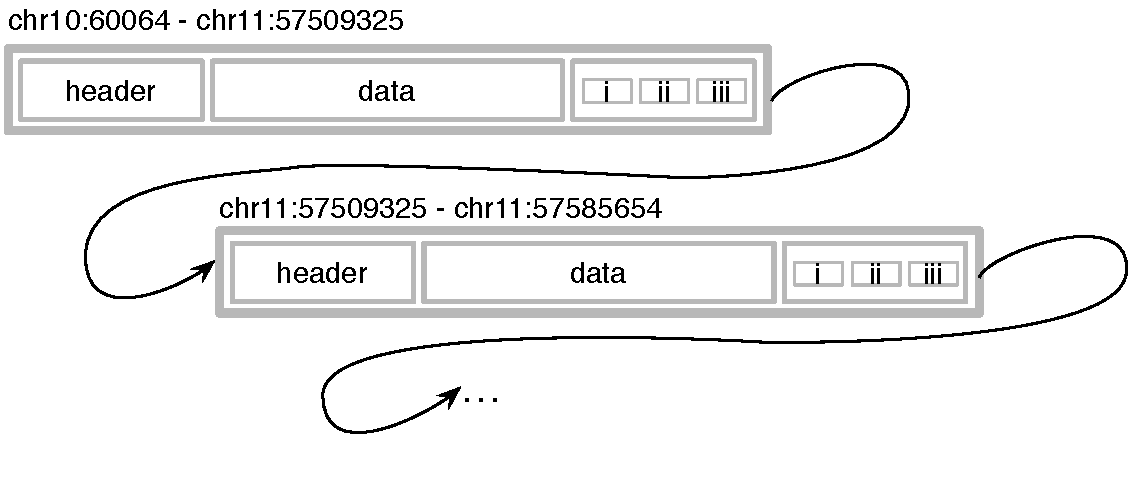
\includegraphics[width=0.8\linewidth]{figures/block_struct}
    \caption{\textbf{Block structure for the compressed data.} The trailer for each block contains a field used to verify data integrity (i), the size of the decompressed data (ii), and, as its last integer (iii), the size of the compressed block (iii). Each block has a genomic interval associated with it that gets recorded in an index.}
    \label{fig:referee:block_struct}
  \end{figure}
  %
  % index file mapping between the blocks and genomic coordinates
  % interval trees for every chromosome/transcript to be able to easily locate the needed block
  When decompressing the data, \refer first traverses the compressed stream and, for each block, reads its size as recorded in the block's trailer and calculates its offset relative to the beginning of the stream. \refer then reads the index file and, for each separate stream and a reference string, builds an interval tree that maps genomic coordinate intervals to the corresponding blocks of compressed data.

  When quering for data on chromosome $C$ within a $[x_1, x_2]$ interval, \refer first locates the interval tree within the stream of offsets that is associated with chromosome $C$ and then enqueues all blocks of compressed offsets blocks that overlap the $[x_1, x_2]$ interval. The enqueued blocks may span an interval $[y_1, y_2]$ that contains $[x_1, x_2]$ completely and  $y_1 <= x_1$ and $x_2 <= y_2$, however, if the interval tree contains no data at $x1$, the initial coordinate $y_1$ may be greater than $x_1$. We then repeat the operation for all other streams required by the user (sequencing edits, read identifiers, etc.). Since the streams are independent and are compressed separately from each other, there is no guarantee that the block queue for edits or read identifiers will start at the same genomic coordinate as the queue of offset blocks. \refer synchronizes all streams to the $x_1$ coordinate and starts decompressing the alignments in order.


  %%%%%%%%%%%%%%%%%%%%%%%%%%%%%%%%%%%%%%%%
  % Stream dependency
  %%%%%%%%%%%%%%%%%%%%%%%%%%%%%%%%%%%%%%%%
  \begin{figure}[ht]
    \centering
    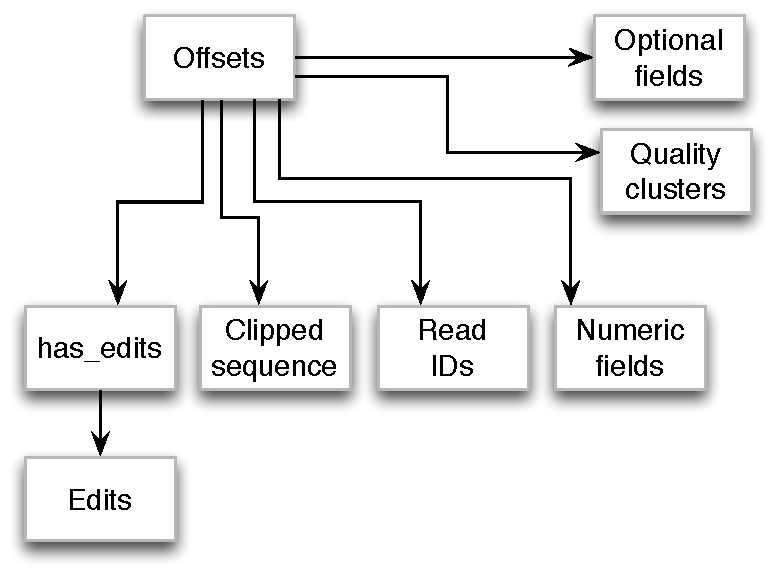
\includegraphics[width=0.6\linewidth]{figures/streams_dependency}
    \caption{\textbf{Dependencies between data streams.} All of the streams depend on the stream of offset data and rely on it to be able to properly compute how many items to skip before begining to decompress data within a compressed block}
    \label{fig:referee:stream_depend}
  \end{figure}

  % currently only supports queries on a single chromosome
  % To allow for random access and partial decompression, \refer builds an index that maps every
  % XXX how does Referee reconstruct reads w/o reconstructing the alignments?

  \refer decompression depends on knowing how many alignments were compressed before any given block. Decompression of any field requires that offsets stream is available to correclty calculate the number of alignments to skip until the begining of interval $[x_1, x_2]$ (see Figure~\ref{fig:referee:stream_depend}).

  % \subsection{Calculating sequencing depth and error rate}

  % We implement two common sequencing operations: depth and error rate estimation procedures. To calculate the depth, the average number of reads aligned over all covered bases, we scan through all offsets and keep track of the last $r$ bases, the  where $r$ is the read length.

%%%%%%%%%%%%%%%%%%%%%%%%%%%%%%%%%%%%%%%%%%%%%%%%%%%%%%%%%%%%%%
%%
%%
%%
%%%%%%%%%%%%%%%%%%%%%%%%%%%%%%%%%%%%%%%%%%%%%%%%%%%%%%%%%%%%%%
\section{Results}

  We introduce \refer which makes global sequence analyses possible without ever fully reconstructing the alignments and further improves SAM compression rates by leveraging separability of data within alignments. \refer performs common tasks at speeds orders of magnitude faster than those for similar tasks within \texttt{samtools} package~\cite{SamTools} and compresses data in times comparable to existing alternatives. \refer operates by grouping related data and converting it into its more compact representation, then passing it down to a general-purpose dictionary coder like \texttt{plzip} for further compression. \refer can compress sequence data down to 0.06 bits per base (a 33x improvement over 2-bit encoding for the same data), its total compressed sizes can be as small as $1/10$ of the original SAM file or up to $50\%$ smaller than an equivalent BAM file. On average, \refer achieves an 8.1\% improvement over the next best approach~\cite{Sahinalp2015}. \refer reduces the size occupied by quality values by identifying highly similar quality vectors in a streaming fashion and encoding them separately from the rest of the qualities. \refer can compress a 13.5Gb SAM file to 1.5Gb in about 10 minutes and while using less than 2Gb of memory. It is highly parallelizable and can be made significantly faster by allowing it to use more threads and memory. When operating on sequencing data exclusively, \refer can process the same 13.5Gb file in under three minutes requiring $<$100Mb of disk space to losslessly represent aligned sequences, a two- to fourfold improvement over competing approaches. Global statistics like depth of coverage can be computed using these compressed sequence data alone and take 44 seconds for a 72Gb SAM file as opposed to 48 minutes when performed by \texttt{samtools}.


  % test data for referee

  We test \refer on a human and bacterial RNA-seq and human whole genome sequencing (WGS) data with varying number of alignments, depth of coverage, error rates, and read lengths (Table~\ref{tab:datasets}). We generated alignments for \texttt{SRR445718} and \texttt{SRR1294122} using STAR~\cite{DobinSTAR}, a fast multi-threaded mapper, with different error rate cutoffs (see later sections).
  \texttt{K562\_cytosol\_LID8465\_TopHat\_v2}, \texttt{NA12878\_S1} datasets are available from EMBL-EBI's ArrayExpress data repository, accession numbers \texttt{ERX283488} and \texttt{ERX237515} correspondingly;
  \textit{P. aeruginosa} was available for download alongside with DeeZ~\cite{Sahinalp2015}. All alignment files were sorted and converted into SAM format using \texttt{samtools}~\cite{SamTools}. Experiments were performed on a Dell PowerEdge T620 machine with 256Mb of RAM.

  \begin{table}[ht!]
    \caption{\textbf{Test set of SAM files.} Experiments were performed on human and bacterial RNA-seq as well as human whole genome sequencing data (WGS) for reads of different lengths. All datasets, except K562, had a significant number of unaligned reads, varying in depth of coverage and error rates. Datasets mostly comprised of Illumina (I) sequences with one exception (Solexa, S). Error rate was calculated as an average number of edits (clipping, indels, splices, and mismatches) over all aligned bases. Sequencing depth was calculated as the average number of aligned reads over the covered bases.}
    \label{tab:datasets}
    \centering
    \begin{tabular}{l l r r r c r}
    \toprule
    File 			& Type 		& $|r|$ & Alignments & Unalign. & Error rate & Depth \\
    \midrule
    % SRR445718 		& RNA-seq 	& 100 & 31892550 & 5677563 \\
    SRR445718, I		& RNA-seq & 100 & 35677496 & 5677563 & 2.85 & 32.67 \\
    SRR1294122, I 		& RNA-seq	& 101 & 47933574 & 1859223 & 1.95 & 21.51 \\
    P. aeruginosa, S 	& RNA-seq	& 51  & 83412201 & 5560731 & 1.04 & 687.19 \\
    K562, I 			& RNA-seq	& 76  & 246476391 & 0 & 1.20 & 73.53 \\
    NA12878\_S1, I 	& WGS 	& 101 & 1015694132 & 202874775 & 1.50 & 36.11 \\
    \bottomrule
    \end{tabular}
  \end{table}

  %%%%%%%%%%%%%%%%%%%%%%%%%%%%%%%%%%%%%%%%%%%%%%%%%%%%%%%%%%%%%%%%%%%%%%%%%%%%%%
  % \subsection{De novo compression performance}

  % XXX --- need to write this whole thing

  %%%%%%%%%%%%%%%%%%%%%%%%%%%%%%%%%%%%%%%%%%%%%%%%%%%%%%%%%%%%%%%%%%%%%%%%%%%%%%
  \subsection{Compression performance on sequence}


  % XXX talking about sequence -- possibly move to sequence section
  % \refer performance on RNA-seq may be partially explained by its improved sequence compression: \refer compresses RNA-seq sequence data up to 3.5 times better than Deez and up to 8 times better than Quip (details in Table~\ref{tab:seq-compression}).


  %
  % results in the table generated based on run-seq-improvements.sh script
  % use python/parse_seq_logs.py to generate the table
  \begin{table*}[ht!]
    \caption{\textbf{\refer performance.} \refer can compress sequence very efficiently down to 0.06 bits per base (bpb). Sequence sizes are shown in Megabytes.}
    \label{tab:seq-compression}
    \centering
    \begin{tabular}{l r r r r}
    \toprule
    % May 4
    % File & Total bases & \refer (bpb) & Deez (bpb) & Quip (bpb) & Error rate & Depth \\
    % \midrule
    % SRR445718 &  3603436792 & \textbf{86.94 (0.22)} & 298.4 (0.69) & 145.34 (0.34) & 2.72 & 32.67 \\
    % SRR1294122 & 4889234340 & \textbf{85.22 (0.16)} & 268.47 (0.46) & 150.54 (0.26) & 1.96 & 21.51 \\
    % P. aeruginosa & 4337434556 & \textbf{41.66 (0.08)} & 59.2 (0.11) & 359.75 (0.71) & 0.53 & 687.19 \\
    % K562 &  18978688729 & \textbf{57.98 (0.03)} & 258.78 (0.11) & 417.98 (0.19) & 0.92 & 73.53 \\
    % NA12878\_S1 & 99817837824 & \textbf{2730.54 (0.23)} & 4229.62 (0.35) & 5845.28 (0.48) & 1.43 & 36.11 \\
    % May 7th
    File & Total bases &  Referee & Quip & Deez \\
    \midrule
    SRR445718 & 3567749600 & 86.63 (0.20) & 145.34 (0.34) & 298.40 (0.70) \\
    SRR1294122 & 4841290974 & 84.33 (0.15) & 150.54 (0.26) & 268.47 (0.47) \\
    P. aeruginosa & 4254022251 & 41.61 (0.08) & 359.75 (0.71) & 59.20 (0.12) \\
    K562 & 18732205716 & 135.99 (0.06) & 417.98 (0.19) & 258.78 (0.12) \\
    NA12878\_S1 & 101569413200 & 2940.07 (0.24) & 5845.28 (0.48) & 4229.62 (0.35) \\
    \bottomrule
    \end{tabular}
  \end{table*}
  %

  % figure w/ depth and error rates over different files
  \begin{figure}[ht!]
    \centering
    % \includegraphics[width=\linewidth]{seq_vs_depth_error}
    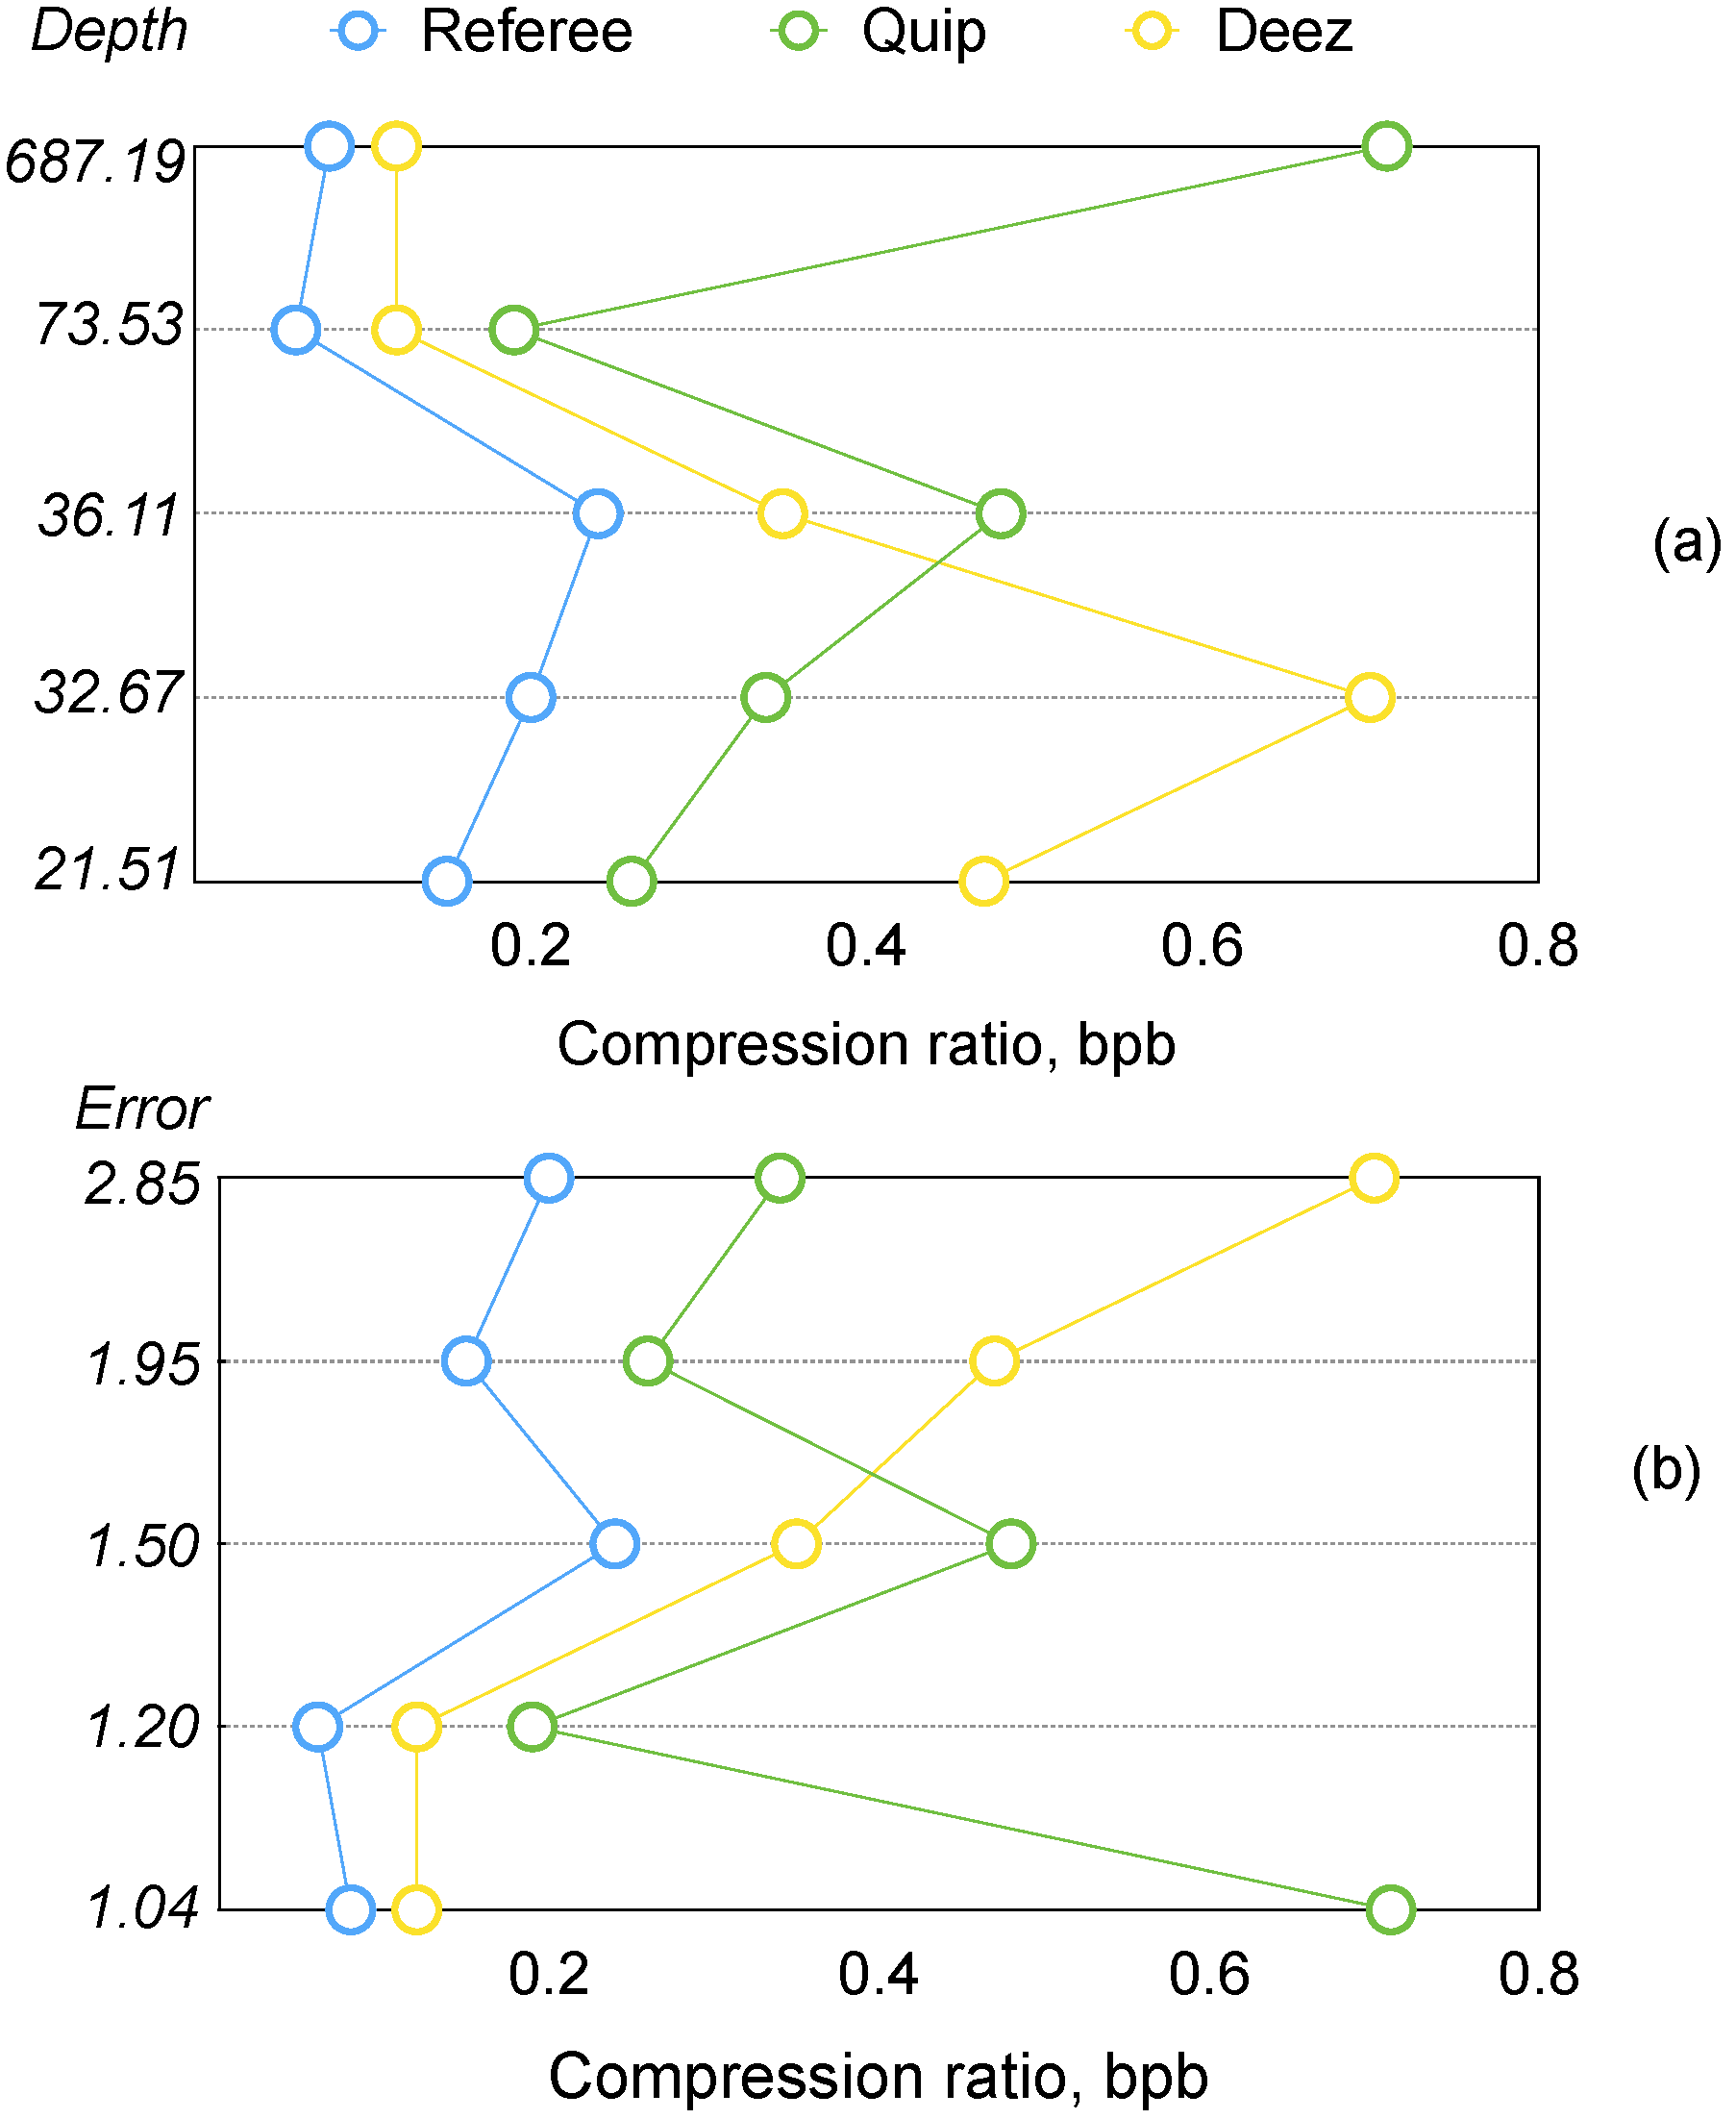
\includegraphics[width=0.6\linewidth]{figures/referee_fig1_complete}
    \caption{\textbf{\refer outperformed both Quip and Deez in sequence compression}: \refer handles increasing error rates and sequencing depths better than its competitors. Deez's rates deteriorate with increasing error rate and Quip's rates tend to be significantly affected by the sequencing depth. Each line in the plots represents a single file; files correspond to those in Table~\ref{tab:seq-compression}.}
    \label{fig:referee:depth-error}
  \end{figure}

  \refer achieves significantly better compression rates for sequencing data within alignments over other competing methods (see Table~\ref{tab:seq-compression}), especially on datasets at high depth of coverage and low error rates. To compare \refer performance to other tools on only the aligned sequence, we replaced read identifiers, quality values, and non-essential fields with default values. We further modified Deez to produce additional debugging information on the size of each stream and ran Quip in a verbose mode. Since both tools could retain some information from other SAM file columns or build indices to allow for fast data access, we only report the sizes for compressed streams that were directly relatable to sequence and not the total size of the file on disk (\texttt{seq} for Quip and the sum of \texttt{seq} and \texttt{edits} for Deez, see Table~\ref{tab:seq-compression}). For \refer, we report a sum of stream sizes for alignment offsets, clipped prefixes and suffixes, and edits. \refer surpasses both Deez and Quip for every dataset leaving a considerable margin.

  % To demonstrate the efficiency of our sequence encoding scheme, we performed an experiment where we compared SAM and \refer ways of encoding sequence (see Table~\ref{tab:seq_comp}). For two RNA-seq runs, we generated alignments with optional MD string and extracted reference names, offsets, cigar and MD strings for each file --- the four columns that completely represent the read sequence (ignoring the clipped regions). Compressing these four columns resulted in improvement of 83\% and 75\% correspondingly over the 2-bit encoding of the read sequences with \refer's format reducing the compressed size further almost twofold.


  The \refer compression rates of bits spent to encode a single base vary from 0.06 to 0.24 --- up to 66 times better than a straightforward 2-bit sequence encoding and up to 8 times better than the two competing methods. In section~\ref{sec:seq-comp-methods}, we discussed how sequence compression quality can be related to read length and should be more effective on longer reads, however, our results show that other factors, like error rate and depth of coverage, can significantly affect the predicted performance (Table~\ref{tab:seq-compression}). We observe that \refer and Deez scale up well with increasing depth of coverage (Figure 1(a)) while Quip's rates drastically go up for the deep sequencing dataset \textit{P. aeruginosa}. \refer achieves best performance for the two datasets with the highest coverage, \texttt{K562} and \textit{P. aeruginosa}, which can be explained by the fact that these also happen to be the two datasets with the lowest error rates. Indeed, compression rates for \refer's and Quip start to decrease slowly as error rates increase --- these two tools are more robust to changes in error rates than Deez for which compression rates quickly deteriorates at higher error rates (Figure~\ref{fig:referee:depth-error}b).
  %
  % When error rate is at its lowest, bit/base ratio is about half that of the ratio at the highest error rate for the RNA-seq data (Figure~\ref{fig:seq-errors}). For example, the two datasets with the best bit per base ratio are also the ones with the shortest read length (\textit{P. aeruginosa} and K562 RNA-seq data), however, \refer is able to capitalize on their sequencing depth and low error rate.


  % compression ratios (bpb) when varying the error rate
  % figure generated by script seq_rates_over_error.py, takes in analysis/seq_bit_per_base_over_error.txt
  % That can be regenrated by referee_error_rates.py and parse_compr_rates_error_rate.py;
  % \begin{figure}[ht]
  % 	\centering
  % 	\includegraphics[width=\linewidth]{seq_rates_over_error}
  % 	\caption{\refer consistently outperforms its competitors in sequence compression, even as error rate increases. Blue: experiments for SRR445718 alignments, green: experiments for SRR1294122 alignments with various allowed error rates. Circles represent \refer, stars --- Deez, and pentagons --- Quip.}
  % 	\label{fig:seq-errors}
  % \end{figure}


  \refer also compresses sequence more efficiently than CRAM~\cite{CRAM}, the first work to consider reference-based sequence compression, for the same depths, error rates, and read lengths. CRAM estimates the bpb ratio to be between 0.175 and 0.20 for unpaired 100bp reads at 1\% error rate and sequencing depth of 25. However, \refer achieves a ratio of 0.14bpb at a higher error rate and similar coverage. As error rates decrease, \refer compression rates improve and are comparable to the rates for 200 and 400 base long reads reported by CRAM (see Figure 2 in~\cite{CRAM}).

  % XXX \refer offers sequence compression rates that are comprable to those reported by CRAM Tools~\cite{CRAMTools} at higher error rates. XXX -- need to run CRAM?



  % In general, we can always expect an improvement in total compression rate over aligned and unaligned sequences to follow a trend $r_a \alpha + r_u (1-\alpha)$ where $\alpha$ is the percent of the reads that successfully aligned and $r_a, r_u$ are compression rates for the aligned and unaligned sequence correspondgly. Whatever the $\alpha$, the savings $(r_u - r_a)\alpha$ may result in large savings in disk space and minutes or hours of the download times.

  % XXX --seq option -- do not encode anything else, just offs, edits, clips, separate timing

  %%%%%%%%%%%%%%%%%%%%%%%%%%%%%%%%%%%%%%%%%%%%%%%%%%%%%%%%%%%%%%%%%%%%%%%%%%%%%%
  \subsection{Compression performance on alignment data}

  \refer outperformed its competitors on all but one test cases, saving hundreds of megabytes in each case. Compared to the original plain text SAM format, \refer offers seven- to tenfold improvement in storage; or up to twofold improvement over its binary variant BAM.
  Our results show that \refer can effectively compress alignments from a wide range of depths of coverage: \refer achieves equally good performance on bacterial \textit{P. aeruginosa} sequenced at an average depth of 687 and human RNA-seq \texttt{SRR445718} dataset with average depth of coverage of 32.
  % XXX discuss error rate performance

  \refer performed significantly better than Deez on human RNA-seq data where alignments contained a significant number of splicing events and achieved a modest improvement for the bacterial RNA-seq alignments. Quip's performance paralleled that of \refer on two of the smaller human RNA-seq datasets, but Quip spent an additional gigabyte encoding alignments for the large \texttt{K562} RNA-seq dataset. \refer had an additional 272Mb over Quip for the human whole genome sequencing dataset, however, it required 600Mb less than Deez to encode the same information.

  Quality values contributed significantly to the size of the compressed data adding up to us much as 80\% of the total compressed size (Figure~\ref{fig:fields}). At the same time, sequencing data took no more than 5.6\% across all datasets with read identifiers and unaligned reads contributing most significantly to the overall size after qualities.

  % (XXX -- update results after applying cigar to the qual cores and with Mincing for unaligned reads)

  % XXX We do not compare to CRAM Tools and Scramble since they result in loss of inofrmation while \refer uses a fully lossless approach.

  % forcing to appear earlier!
  % run compute_sizes.sh on ocean:/mnt/scratch1/dfilippo/aligned to get the sizes
  \begin{table*}[ht!]
    \caption{\textbf{Comparison between BAM/SAM compression methods and \refer on human RNA-seq, bacterial and human WGS datasets.} The second number for \refer indicates \% improvement over the next best approach. The sizes are reported in megabytes.}
    \label{tab:compression}
    \centering
    \begin{tabular}{l r r r r r}
    \toprule % Deez Refere Bam Quip
    File    		& Referee (\%) & Quip 			& Deez 		& BAM  & SAM \\
    \midrule
    SRR445718       & \textbf{1242.67} (8.30\%) & 1355.5 & 1607.11 & 2282.45 & 9544.98 \\
    SRR1294122      & \textbf{1545.15} (10.7\%) & 1730.15 & 2022.63 & 3107.67 & 13650.17 \\
    P. aeruginosa   & \textbf{1866.87} (2.80\%) & 2180.95 & 1921.06 & 3339.54 & 19008.37 \\
    K562    & \textbf{7147.04} (10.6\%) & 8274.43 & 7997.7 & 13119.44 & 72398.19 \\
    NA12878\_S1     & 62176.53 (-0.4\%) & \textbf{61904.65}  & 62774.92 & 108289.6 & 437589.43 \\
    \bottomrule
    \end{tabular}
  \end{table*}


  %%%%%%%%%%%%%%%%%%%%%%%%%%%%%%%%
  %%
  %%%%%%%%%%%%%%%%%%%%%%%%%%%%%%%%
  \subsection{Quality values compression performance}

  % \# of clusters, cluster sizes, compression rates per cluster vs the general pile.
  % + How many items were in some cluster vs. generic pile?
  % - How well did clusters compress?
  % - Specificl clusters: best quality values, worst quality values.
  % - Separating prefixes \& suffixes -- clustering improves; compression improves.

  Although high variability of quality values makes them notoriously hard to compress, \refer's clustering scheme results in 13 to 17\% reduction in compressed size for quality values over \texttt{plzip} without a significant increase in runtime or memory used. Across the tested datasets, \refer performs similarly or better than arithmetic coding (AC) schemes employed by Deez and Quip (see Table~\ref{tab:qual-compression}) while making partial decompression feasible.
  For quality vectors that get placed into clusters, the average compression rate lies between 6.2 and 10.9. Combined with a considerably lower compression ratio for the quality vectors placed in the generic pile, the overall compression rate for qualities varies between 3.33 and 4.22 on the tested datasets.

  The number of quality clusters did not exceed four (including the generic pile) with the number of vectors assigned to non-generic clusters ranging from 31 to 67\% over all datasets. For most datasets, two clusters formed consistently: a cluster of vectors consisting of mostly the highest quality value and a smaller cluster of vectors consisting almost entirely of the lowest quality value. For vectors in clusters, collections of core substrings compressed down to $1/3 - 1/4$ of the original size. In general, quality vectors compressed better when separated into prefixes, cores, and suffixes as opposed to vectors that were not split, e.g. clusters for \texttt{SRR1294122} before separation would compress at 5.6, 5.7, and 4.5 ratios, but with prefixes and suffixes compressed separately the compression rate over the three clusters increases to 6.3, 6.6, and 4.8 correspondingly.

  % to generate table:
  \begin{table}[ht!]
    \caption{\textbf{\refer streaming clustering approach improves quality values compression} across most of the tested datasets (sizes reported in Megabytes).}
    \label{tab:qual-compression}
    \centering
    \begin{tabular}{l r r r}
    \toprule
    File & \refer & Deez & Quip \\
    \midrule
    SRR445718 	& \textbf{976.76} & 1055.70 & 984.54 \\
    SRR1294122 	& \textbf{1092.92} & 1328.17 & 1226.99 \\
    P. aeruginosa & 1160.75 & 1084.87 & \textbf{994.1} \\
    K562 		& \textbf{5358.94} & 5830.98 & 5715.71 \\
    NA12878\_1 	& \textbf{32560.26} & 38413.76 & 38097.35 \\
    \bottomrule
    \end{tabular}
  \end{table}

  % \refer's streaming approach improves on the arithmetic coding quality compression rates reported by Deez and Quip (see Table~\ref{tab:qual-compression}), however, block-wise encoding makes random access feasible.  To obtain compressed size for quality values achieved by Deez and Quip, we used the auxilary output produced by Deez and ``-v'' option for Quip. Deez was run with default options (lossless compression).



  % than collections of mixed quality vectors with compressed clusters occupying up to 37 times less space than the uncompressed quality vectors.

  % XXX Separating the prefixes and suffixes from the core substring results in further compression since prefixes and suffixes within a cluster tend to largely repeat from vector to vector.

  %%%%%%%%%%%%%%%%%%%%%%%%%%%%%%%
  %%
  %%%%%%%%%%%%%%%%%%%%%%%%%%%%%%%
  \subsection{Separable streams and random access}

  % XXX discuss stream separability; partial decompression/random access. operations can be done on offsets alone; offests and edits. Expect sequence to be of most interest.

  % XXX explain how separable streams benefit the user

  Dividing similar data into separate data streams allows \refer to compress data more efficiently due to increased data homogeneity. To highlight efficiency of encoding data in separate streams, we performed the following experiments: for every alignment in the SAM file, we extracted columns for reference identifier (RNAME), offset (POS), CIGAR and MD strings and compressed them using a command-line tool. We then grouped reference identifiers with offset column in one file and CIGARs with MD strings in a separate file and compressed these two files using a command-line tool. Lastly, we applied \refer encoding to the four columns and report the summary size of all resulting streams. Data required to encode clipped regions was computed separately and added to each experiment's total size (20.79Mb and 13.37Mb for the \texttt{SRR445718} and \texttt{SRR1294122} correspondingly). Results are summarized in Table~\ref{referee:table:progressive_enc}: compressing the four columns that completely describe the sequence introduces a 6--8 times improvement over 2-bit encoding and \refer improves that ratio to 10--12 range.

  \begin{table}
    \centering
    \begin{tabular}{l r r r r r }
      \toprule
      File & Bases & 2bit & SAM/4 & SAM/2+2 & \refer \\
      \midrule
      % % plzip -- includes clipped regions
      % SRR445718   & 3,422,790,818 & 855,697,705   & 140,098,256 & 85,257,945\\
      % % plzip
      % SRR1294122  & 4,343,436,421 & 1,085,859,106 & 143,307,769 &  88,170,914 \\
      % plzip -- includes clipped regions
      SRR445718   & 3,422,790,818 & 815.06 & 133.61 & 104.00 & 86.94 \\
      % plzip
      SRR1294122  & 4,343,436,421 & 1035.56 & 136.67 & 103.77 & 85.22 \\
      \bottomrule
    \end{tabular}
    \caption{\textbf{Progressive compression improvements when compressing sequence-related fields.} Compressed with \texttt{plzip}. SAM/4 represents the size of RNAME, POS, CIGAR, and MD string in a column format, compressed. SAM/2+2 represents the total size of RNAME, POS columns compressed along with CIGAR, MD string columns compressed. Unaligned sequences were not included in the analysis; sizes are reported in Mb, unless otherwise indicated.}
    \label{referee:table:progressive_enc}
  \end{table}

  In addition to improved compression, streams can be downloaded separately since they are largerly independent of each other. For most sequence analyses, the user would only need to download the offsets stream (see Figure~\ref{fig:referee:stream_depend} for a scheme of dependencies). Subsection~\ref{sec:referee:random_access} goes over the organisation of the streams and indexes in detail.

  Finally, the reduced size of sequence stream and its simple organization allow one to perform certain sequence-focused analyses orders of magnitude faster than comparable tasks done with, e.g. \texttt{samtools}~\cite{SamTools}. A common task such as computing a dataset's sequencing depth involves going through all alignments while recording the number of reads aligned to any covered base. \texttt{samtools depth} takes about 19 minutes to compute depth for a modestly sized \texttt{SRR445718} dataset and over 48 minutes for \texttt{K562} while \refer accomplishes that same task in 8 and 44 seconds correspondingly. The difference is explained by the fact that \texttt{samtools} has to scan through all of alignment data, including data unrelated to depth calculation, while \refer accomplishes the same task by  having to go through compressed offsets (about 5\% of the compressed data).

  
  Likewise, \refer format allows one to quickly reconstruct aligned reads originally embedded in SAM file (an equivalent of \texttt{samtools faidx} command) without ever reconstructing the alignments fully. Users can specify a genomic region of interest and \refer can reconstruct alignments from that genomic region without decompressing the whole dataset. The index that \refer constructs to enable partial decompression is lightweight: for example, to index all data blocks for \texttt{NA12878}, \refer uses 1.2Mb which can be further compressed down to 233Kb --- a size negligible when compared to the size of the data itself.

  % XXX compare to Deez's random access speeds 

  % / time to perform certain analyses


  %%%%%%%%%%%%%%%%%%%%%%%%%%%%%%%
  %%
  %%%%%%%%%%%%%%%%%%%%%%%%%%%%%%%
  \subsection{Speed and memory demands}

  \refer is fast and only requires on the order of 1.5Gb of RAM to run making it usable on even smaller machines (see Table~\ref{tab:runtimes}). \refer streams through the alignments in a sequential fashion only keeping intermediate information in memory before it is passed on to \texttt{lzlib}. \refer launches several threads that each invoke \texttt{lzlib} operations on a single block of data at a time making use of modern multithreading architectures. \refer will run faster if given more processing power, however, \refer can reach a saturation point where data blocks prepared by \refer are compressed at a faster rate than the new blocks are being produced.

  % XXX add timing information for when only compressing sequence

  % XXX how is referee parallelized

  % XXX does it scale up linearly w/ \# CPUs, memory?

  % XXX fill out the table -- timing information, memory (Figure~\ref{tab:runtimes})

  % generated by script python/parse_timings.py
  % relies on the usr/bin/time -v and logs for each file, tool
  \begin{table}[ht]
    \caption{\textbf{\refer is comparable or faster to the other competing tools.} We report wall running times and \% of CPU used by each tool. Both Deez and \refer were run with 10 threads, Quip was run in its default mode since it does not offer a multithreaded functionality.}
    \label{tab:runtimes}
    \centering
    % \begin{tabular}{l r r r r}
    % \toprule
    % File & \refer & Deez & Quip -r & sam2bam \\
    % \midrule
    % SRR445718 		& 9m 	&	16.3m 	& - & -\\
    % SRR1294122 		& 7m 	& 	7.7m	& 5m32s & - \\
    % P. aeruginosa 	& 11m13s&	7.1m 	& 7m07s & - \\
    % K562 			& -		& 	- 		& 27m32s & - \\
    % NA12878\_S1 	& 5h18m & 5h49m 	& - & - \\
    \begin{tabular}{l r r r r }
    \toprule
    File & Referee & Deez & Quip -r \\
    \midrule
    SRR445718 		& 7:05 (1017\%) & 10:34 (190\%) & 6:59 (139\%) \\
    SRR1294122 		& 10:26 (1016\%) & 11:07 (204\%) & 7:48 (149\%) \\
    P. aeruginosa 	& 18:41 (608\%) & 7:34 (163\%) & 9:18 (153\%) \\
    K562 			& 54:09 (620\%) & 50:07 (180\%) & 36:06 (157\%) \\
    NA12878\_S1 	& 5:18:12 (828\%) & 3:00:08 (190\%) & 3:13:31 (164\%) \\
    \bottomrule
    \end{tabular}
  \end{table}

  \refer could be run in a lossy manner in which only the essential information about sequence and alignment is recorded and information like read identifiers, flags, quality values, and optional SAM fields are not stored. Users can enable this mode by providing an optional ``\texttt{--seqOnly}'' parameter: \refer would encode offsets and edits for every alignment it incurs along with the unaligned reads. Alternatively, users can further restrict \refer to only encode primary alignments by using a ``\texttt{--discardSecondary}'' option. Since \refer has to look over less data, sequence only mode is much faster than the lossless operation: for example, the sequence in either of the three smallest RNA-seq datasets can be compressed in under 3 minutes.

  % XXX a paragraph that discusses speed to decompress, including random access

  Given the fact that modern mapping tools can generate alignments in a matter of minutes even for large files, the ``\texttt{--seqOnly}'' options make \refer a reasonable choice when the goal is to compress sequencing data. Indeed, an  aligner like STAR~\cite{DobinSTAR} can process 11Gb human RNA-seq dataset (e.g.\@ \texttt{SRR1294122}) in under five minutes generating alignments for $94.31\%$ of all reads. \refer takes under three minutes to compress the resulting SAM file with ``\texttt{--seqOnly --discardSecondary}'' options encoding the aligned reads in 2.1\% of their original size and the unaligned reads in 25\% of their original size. Overall, this combined scheme encodes all of the 39.7 million of original reads in 3.3\% of their original size requiring only eight minutes to do so. Considering \refer's consistently good performance at different error rates (Figure 1), we conclude that for the purposes of sequence compression, it is reasonable to trade off the quality of alignments for the number of aligned reads.




%\section{Results}

%%%%%%%%%%%%%%%%%%%%%%%%%%%%%%%%%%%%%%%%%%%%%%%%%%%%%%%%%%%%%%%%%%%%%%%%%%%%%%%%
\section{Discussion and Conclusions}

We present a novel approach for efficient compression and storage of the  alignment information that enables certain computational analyses without ever having to decompress the data fully. \refer operates by separating related streams of data and encoding them individually thus achieving better compression rates on each stream. \refer is competitive in speed and performance to other state of the art tools that employ more complex compression schemes~\cite{Sahinalp2015,Jones2012}. We show that \refer can compress alignment data down to $1/10^{th}$ of its original SAM file size. When focusing only on sequence data (i.e., stripped of extraneous information like read identifiers), \refer can compress it in a lossless manner 2 to 9 times better than the competing methods (see Table~\ref{tab:seq-compression}). \refer's efficient encoding of mapping locations and sequence variation makes it robust to increasing error rates (Figure~\ref{fig:referee:depth-error}). Coupled with the fact that modern alignment tools can successfully map millions of sequencing reads in minutes, \refer becomes an appealing choice in sequence compression, especially for the rapidly growing body of RNA-seq and WGS datasets for the model organisms for which well-annotated reference genomes are available.


Many analyses relying on the alignment information do not require original read identifiers or unaligned reads focusing instead on the sequence that aligned successfully. In such cases, being able to download only the data one needs may significantly reduce the download size. \refer separates data streams into distinct compressed files and only requires a subset of them to reconstruct the original SAM/BAM data. Read identifiers, quality values, optional SAM fields and all of the unaligned reads can be skipped, reducing the download size by 84-93\% (see Figure~\ref{fig:fields}).

% Modular design: requires only essential fields: offsets, mapping flags, edits+clipped regions. Can skip: read ids, qualities, opt. fields, unaligned reads.

\begin{figure}[ht!]
  \centering
  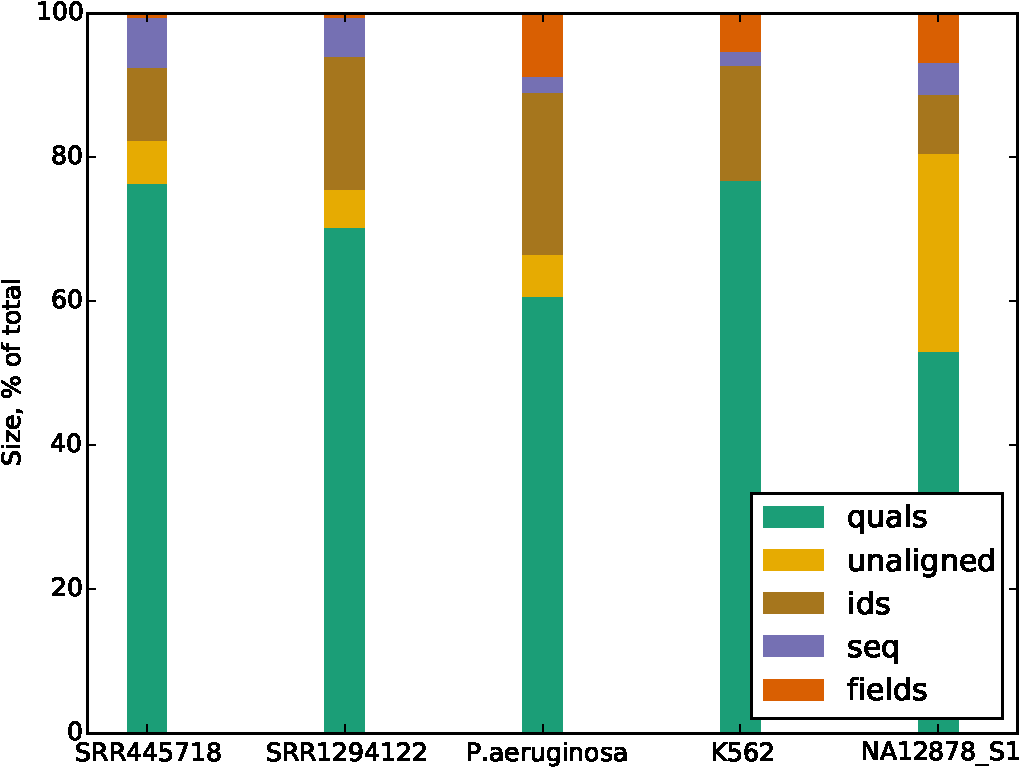
\includegraphics[width=0.6\linewidth]{figures/Referee-size-breakdown-May4}
  \caption{\textbf{Compressing streams separately allows to download them independently.} Quality values and read identifiers contribute significantly to the size of the compressed file, however, \refer does not rely on these data to reconstruct sequence alignments. Omitting the non-essential alignment data can reduce the size of the download by up to 93\%.}
  \label{fig:fields}
\end{figure}

% XXX: merging sequence?


% \refer is written in C++ and is available on GitHub (\url{https://github.com/Kingsford-Group/referee}).

%%%%%%%%%%%%%%%%%%%%%%%%%%%%%%%%%%%%%%%%%%%%%%%%%%%%%%%%%%%%%%%%%%%%%%%%%%%%%%%%
%%
%% Overall conclusions
%%
%%%%%%%%%%%%%%%%%%%%%%%%%%%%%%%%%%%%%%%%%%%%%%%%%%%%%%%%%%%%%%%%%%%%%%%%%%%%%%%%
\chapter{Discussion and Conclusions}

% XXX go over projects

In this dissertation, we present algorithmic and visualization challenges that arise when storing, trasmitting, and interpreting high-throughput biological data. We explore a variety of datasets from protein-protein interaction networks to dynamic networks of relationships between individuals to sequencing data. The tools developed to address these challenges allow one to operate on these data more efficiently, guiding attention towards potential insights, and can be used beyond their intended applications to biological data.

In Part~\ref{part:vis}, we focus on visualization tasks for large complex biological data and address several specific problems. We develop targeted views that allow to explore multiple clusterings of a PPI network at a high-level, to seamlessly narrow down a set of proteins of interest and study such sets in greater detail within the context of a single application. To automatically extract insights, we designed an algorithm that identified subsets, or \textit{cores}, of proteins for which the annotations persisted across multiple annotation schemes. 
% why was coral important? limitations, future work?
Our analysis of the \textit{A. thaliana} protein-protein interaction network suggests that relying on a single set of annotations may significantly skew the analysis and users should always seek multiple alternative clusterings and consider them en masse. It is particularly important in light of the fact that high-throughput biological data may contain experimental noise and results may vary due to the nuances of the experimental protocols.
% map of jazz -- kinda in passing
Separately, we explored a setting where network data was changing over time. We propose to focus on visualizing the local structure with an option of viewing more of the network data. We developed a novel layout that allowed to observe the egonetwork over several timepoints while minimizing amount of unnecessary changes between consecutive timesteps. Our work has implications for longitudinal analyses of dynamic networks.

We extended the core finding algorithm to chromatin conformation data to identify persistent subsets of interactions representing \textit{topological domains} --- robust 3-dimensional structures within nucleus of living cells. Topological domains have been implicated in long-range gene regulation, appear to be significant building blocks in genome packing and affect DNA accessibility. Our algorithm finds optimal solutions to the problem and has since been extended to explore the space of alternative optimal and near-optimal solutions. Its ability to extract domains at different resolutions have provided first quantitative evidence that nuclear chromatin is organised in a hierarchical fashion.



In Part~\ref{part:compress}, we develop new strategies and algorithms for sequence and alignment data compression. We define a general problem of extracting information shared between sequencing datasets originating from the same species, environment, or experiment. We proposed to use such shared information to compress files within a single collection of related data. We consider a set of most frequently occuring kmers as one such example of shared information and develop algorithms for efficiently derive such kmer sets given an input sequence (or sequences). Separately, we consider a problem of optimally encoding a sequence given such collection of kmers and their compressed representations. We observe that kmer sets are too diverse to produce a succinct shared data structure, even when they originate from the sequencing reads derived on the same species and using the same experimental protocol. However, the same reads successfully map to the common reference genome, which suggests that reference is a better example of shared information. We are able to achieve better compression for datasets with varying sequencing error rates. We improve state-of-the-art compression ratios for reference-based compression tools and provide an implementation of our method that allows for random access to original data without fully decompressing the original, which allows us to compute sequence-specific analyses orders of magnitude faster than on the original data with an added benefit of modular downloads and direct computation on the compressed data.

% XXX Russell -- does it matter how good the alignments are? for instance, if you're seuqencing an organism that has no reference genome but you have a homology, are you better off doing reference-based compression to the homology or just reference-free? Answer: can discuss in the limitations.

% We conclude that collections of kmers may be a suboptimal data structure to encode shared information, especially when compared to compression performance in reference-based setting.

% highlight contributions

% stress potential impact

% outline some future developments for each contribution?

% xxx applications of map of jazz to biological networks
% XXX local structure in map of jazz vs global changes

% \section{Limitations}

% XXX: Russell --- discuss limitations

% Coral

% Map of Jazz

% Domains -- account for hierarchy directly

% Compression -- reference-based is limited in that you need to have ther reference available. Computing reference -- mini contigs (like Quip)

\section{Future work}

In chapter~\ref{chapter:mapofjazz}, we used a social network to discuss visualization strategies for dynamic networks, however, the same strategies could be used to track changes in gene-gene interactions~\cite{GeneKnockouts} over a period of time or changes in a microbial gut ecosystem over a course of treatments. Our assumption that a local view is preferable to the global overview of the changing network can be tested by conducting a usability study in a controlled environment where users are asked to perform a series of tasks testing their ability to extract insights using a local view such as a Map of Jazz versus a global view such as Net EvViz~\cite{Khurana2011}. One would have to take into account network size, degree distribution, number of timepoints and the time span, as well as amount of change the network undergoes between any two consecutive time points.
% We conjecture that for some tasks, such as assessing overall changes for a single node and its neighborhood, Map of Jazz will be easier to 

Map of Jazz focuses user's attention on temporal changes in a subnetwork, however, locally observed changes may not be fully reflective of the global dynamics. While node and edge widgets provide a degree of information about a global state of the network, the user has to consider other tools to study network-wide changes. An extention to the ``hops'' view that would progressively show more of the ego-network would give users the power to control the amount of network information they want to see.

Our formulation for identification of topological domains in chromatin considers domains at different scales separately and does not make any assumptions about its hierarchical nature. The hierarchy is strongly suggested by our findings when analysing alternative optimal and near-optimal solutions~\cite{ArmatusAMB} and by the earlier light microscopy observations of chromosome territories~\cite{Cremer2010}. Incorporating the assumption that domains form a hierarchy directly into the objective will allow to sample from most probable nested structures. Such approach may result in domains sets that are more stable across cell types and could allow for a more principled hierarchy comparisons across species.

Our initial version of functional compression using a reference sequence allows for efficient computations on the sequence stream. Exposing an API to the sequence stream would encourage a broader adoption of our proposed  framework and might result in new sequence computations being developed using \refer's paradigm. Our performance on sequence compression has implications for large-scale sequence analyses: given 2 Petabases of human RNA-seq experiments, the current number of bases in SRA, \refer could compress it down to 48 Terabases (assuming an average compression ratio of 0.29 bpb) allowing one to store all of the data and to run analyses on a single machine.

Reference-based compression is only feasible when a well established genome is available and the sequence in the reads does not differ from the reference in a significant way. However, when the reference genome is not available or when the reads are coming from a related, but divergent sequence, the reference-based compression fails to provide any significant benefit over the \textit{de novo} methods. This situation arises when compressing related species (say, human and chimpanse) or when compressing shotgun metagenomic samples where multiple strains and species from a single genus may be present with sequence similarity close to 100\%. Combining ideas from MINCE~\cite{Mince} where reads are clustered based on the shared minimizer, and Quip~\cite{Jones2012}, where reads are assembled into small contigs, might prove to be a middle ground between the \textit{de novo} and reference-based approaches. The local micro-contigs have to be able to adapt as more reads are placed in the bucket. The feasibility of such compression scheme would have to be compared against other \textit{de novo} approaches and its scalability to large datasets would have to be tested extensively.

% XXX Russell -- it might be interesting to consider what one could do with a ``reference'' consisting of references to a whole population, or even a universal dictionary of known sequences.
% xxx data-driven local micro-references and contigs for data compression in metagenomic data

% \appendix
% \include{appendix}

\backmatter

% need to include boblatex, but then it conflicts with some other package
% \AtEveryBibitem{% Clean up the bibtex rather than editing it
%  \clearlist{address}
%  \clearfield{date}
%  \clearfield{eprint}
%  \clearfield{isbn}
%  \clearfield{issn}
%  \clearfield{month}
%  % \ifentrytype{book}{}{% Remove publisher and editor except for books
%   % \clearlist{publisher}
%   % \clearname{editor}
%  % }
% }

%\renewcommand{\baselinestretch}{1.0}\normalsize

% By default \bibsection is \chapter*, but we really want this to show
% up in the table of contents and pdf bookmarks.
\renewcommand{\bibsection}{\chapter{\bibname}}
%\newcommand{\bibpreamble}{This text goes between the ``Bibliography''
%  header and the actual list of references}
\bibliographystyle{plainnat}
\bibliography{mypapers,references,jazzmap,graph_drawing,dynnetvis,coral_bmc,coredomain,compression}

\end{document}
